%% ----------------------------------------------------------------
%% Thesis.tex -- MAIN FILE (the one that you compile with LaTeX)
%% ----------------------------------------------------------------

% Set up the document
% Location of the graphics files (set up for graphics to be in PDF format)
% Use the "Thesis" style, based on the ECS Thesis style by Steve Gunn
\documentclass[a4paper, 11pt, oneside]{Thesis}
\renewcommand{\familydefault}{\sfdefault}
\graphicspath{Figures/}

% Include any extra LaTeX packages required
% Use the "Natbib" style for the referen:wqces in the Bibliography
% Needed for the "comment" environment to make LaTeX comments
% Allows "\bvec{}" and "\buvec{}" for "blackboard" style bold vectors in maths
% Colours hyperlinks in blue, but this can be distracting if there are many
% links.
\usepackage[square, numbers, comma, sort&compress]{natbib}
\usepackage{verbatim}
\usepackage{vector}
\usepackage{bm}
\usepackage{mathrsfs}
\usepackage{amsmath}
\usepackage{amssymb,array,bm,calc,multirow,diagbox,mathtools}

\usepackage{hhline}

\usepackage{algorithm,algpseudocode}
\renewcommand{\algorithmicrequire}{\textbf{Input:}}
\renewcommand{\algorithmicensure}{\textbf{Output:}}
%\usepackage[ruled, vlined, linesnumbered]{algorithm2e}

\usepackage{graphicx,esint,color}
\usepackage{adjustbox}
\usepackage{tikz}

\usepackage{boondox-calo}

\usetikzlibrary{positioning}
\usetikzlibrary{arrows.meta}
\usetikzlibrary{decorations}
\usetikzlibrary{shapes}
\usetikzlibrary{shapes.geometric}
\usetikzlibrary{shapes.multipart}
\usetikzlibrary{calc}
\usetikzlibrary{arrows, decorations.markings}
% for double arrows a la chef
% adapt line thickness and line width, if needed
\tikzstyle{vecArrow} = [thick, decoration={markings,mark=at position
    1 with {\arrow[semithick]{open triangle 60}}},
    double distance = 1.4pt, shorten >= 5.5pt,
    preaction       = {decorate},
    postaction      = {draw,line width=1.4pt,  gray,shorten >= 4.5pt}]
\tikzstyle{innerWhite} = [semithick, white,line width=1.4pt, shorten >= 4.5pt]
\usepgflibrary{decorations.pathmorphing}
\usepgflibrary{decorations.pathreplacing}
%\hypersetup{urlcolor=blue, colorlinks=true}
\hypersetup{colorlinks,
            citecolor=black,
            linkcolor=black,
            urlcolor=black,
            colorlinks=true}
%
\newcommand{\R}{\mathbb R}
\newcommand{\yH}{\bm y_\text H}
\newcommand{\yM}{\bm y_\text M}
\newcommand{\YH}{\bm Y_\text H}
\newcommand{\YM}{\bm Y_\text M}
\newcommand{\Tr}{^\top}%\newcommand{\Tr}{^\text T}
\newcommand{\Fr}{_\text F}
\newcommand{\iter}[1]{^{(#1)}}
\newcommand{\vectxt}[1]{\texttt{vec}{(#1)}}
\newcommand{\sgn}[1]{\texttt{sgn}{(#1)}}
\newcommand{\thtxt}{^\text{th}}
\newcommand{\inv}{^{-1}}
\newcommand{\etal}{\textit{et al.}\;}
\newcommand{\ie}{i.e.,\,}
\usepackage{stackengine}
\newcommand{\delequal}{\mathrel{\ensurestackMath{\stackon[1pt]{=}{\scriptstyle\Delta}}}}
\usepackage{colortbl}
\usepackage[flushleft]{threeparttable} % for footnote in table

\setcounter{tocdepth}{2}

\captionsetup{font=normalsize,labelfont={bf,sf}}
\captionsetup[sub]{font=Large,labelfont={bf,sf}}

% ---------------------------------- %
% Settings for Importing Matlab Code %
% ---------------------------------- %
%\usepackage[utf8]{inputenc}
%\usepackage{fontspec}
\usepackage{listings}
\definecolor{codegreen}{rgb}{0,0.6,0}
\definecolor{codeblue}{rgb}{0,0,1}
\definecolor{codegray}{rgb}{0.5,0.5,0.5}
\definecolor{codepurple}{rgb}{0.58,0,0.82}
%\definecolor{backcolour}{rgb}{0.95,0.95,0.92}
\definecolor{backcolour}{rgb}{1,1,1}

\lstdefinestyle{mystyle}{
    backgroundcolor   = \color{backcolour},
    commentstyle      = \color{codegreen},
    keywordstyle      = \color{magenta},
    numberstyle       = \tiny\color{codeblue},
    stringstyle       = \color{codepurple},
    basicstyle        = \footnotesize,
    breakatwhitespace = false,
    breaklines        = false,
    captionpos        = b,
    keepspaces        = true,
    numbers           = left,
    numbersep         = 5pt,
    showspaces        = false,
    showstringspaces  = false,
    showtabs          = false,
    tabsize           = 2
}
\lstset{style=mystyle}
\lstset{basicstyle=\linespread{1.2}\footnotesize\ttfamily}
% ----------------------------------------- %
% End of Settings for Importing Matlab Code %
% ----------------------------------------- %



%% ----------------------------------------------------------------
\begin{document}
% Begin Roman style (i, ii, iii, iv...) page numbering
\frontmatter

% Set up the Title Page
\title  {Hyperspectral Super-resolution Using Matrix Factorization}
\authors  {\texorpdfstring
            %{\href{your web site or email address}{CHAN, Chun Hei}}
            {\textbf{CHAN, Chun Hei}}
            {Author Name}
            }
\addresses  {\groupname\\\deptname\\\univname}
% Do not change this here, instead these must be set in the "Thesis.cls" file,
% please look through it instead
\date       {\today}
\subject    {}
\keywords   {}

\maketitle
%% ----------------------------------------------------------------

% It is better to have smaller font and larger
% line spacing than the other way round
\setstretch{1.3}

% Define the page headers using the FancyHdr
% package and set up for one-sided printing
\fancyhead{}                      % Clears all page headers and footers
\rhead{\thepage}                  % Sets the right side header
                                  % to show the page number
\lhead{}                          % Clears the left side page header

\pagestyle{fancy}                 % Finally, use the "fancy" page style
                                  % to implement the FancyHdr headers

% The Abstract Page
\addtotoc{Abstract}               % Add "Abstract" page entry to the Contents
\abstract{
\addtocontents{toc}{\vspace{1em}} % Add a gap in the Contents, for aesthetics

% The Thesis Abstract is written here (and usually kept to
% just this page). The page is kept centered vertically so
% can expand into the blank space above the title too\ldots
Hyperspectral imaging systems have recently drawn significant interest in
areas such as computer vision, signal processing, and remote sensing because
of their ability to provide rich information in both spectral and spatial
domain of a scene.
These imaging systems acquire spectral images from far infrared to visible
range with many spectral bands, resulting in images that have a lot more
spectral bands than that of the conventional multispectral images.
Due to hardware limitation, spectral cameras with high resolution in both
spectral and spatial domain are uncommon, especially in the application of
remote satellite imagery.
The sensors are usually called hyperspectral camera and multispectral camera.
%The sensors are usually hyperspectral camera and multispectral camera, which
%capture images with high spectral and low spatial resolution, and vice versa,
%respectively.

Hyperspectral super-resolution is a problem of fusing a hyperspectral image
and a multispectral image of the same scene to form a full spectral image
having the high spectral resolution of the former and high spatial resolution
of the latter.
In the existing methods, some of them can be classified as matrix
factorization-based methods in which the desired full spectral image can be
expressed as the product of an endmember matrix and an abundance matrix.
The objective of this family of methods is to estimate the endmember-abundance
matrix pair solely from the hyperspectral and multispectral observations.
Conventionally, matrix factorization requires alternating optimization with
respect to each factor matrix individually.
This makes the hyperspectral super-resolution problem an iterative procedure
of solving subproblems with respect to the endmember matrix and abundance
matrix alternatingly.

In this thesis, some matrix factorization-based formulations of the
hyperspectral super-resolution problem are investigated.
In each of the investigation there are two major focus.
The first focus is on the effect of exactness of solving the subproblems
during alternating optimization against the fusion and unmixing performance,
measured by both reconstruction accuracy of full spectral images and the
unmixing accuracy of the endmember-abundnace matrix pair.
The second focus is on the fusion and unmixing performance using a variety of
first order optimization methods for solving the subproblems.

The contribution of this thesis is that a framework of alternating
optimization on matrix factorization is developed.
Simulation results show that by inexactly solving the subproblems, the
hyperspectral super-resolution problem can still be solved to comparable
accuracy but with much less computation time than the state of the art.
}

\clearpage
\begin{centering}
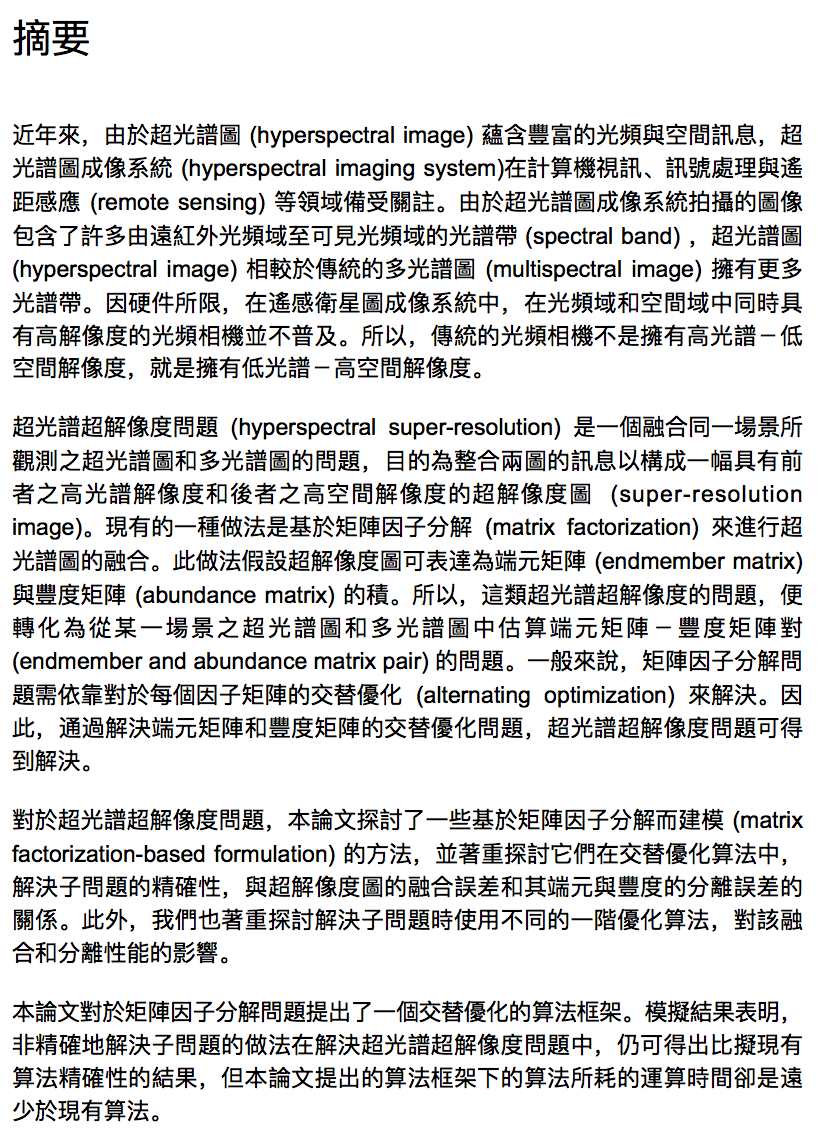
\includegraphics[width=0.98\linewidth]{./fig/abstract_chi/Abstract_chi}
\end{centering}

\clearpage                        % Abstract ended, start a new page
%% ----------------------------------------------------------------

\setstretch{1.3}                  % Reset the line-spacing to 1.3 for
                                  % body text (if it has changed)

% The Acknowledgements page, for thanking everyone
\acknowledgements{
\addtocontents{toc}{\vspace{1em}} % Add a gap in the Contents, for aesthetics

%The acknowledgements and the people to thank go here, don't forget to include
%your project advisor\ldots
~\\
~\\
~\\
~\\
First of all, I would like to greatly thank my supervisor, Prof. Wing-Kin Ma,
for his guidance and advice in my research throughout the past few years in
which I have received great amount of freedom, patience, tolerance and
opportunities in learning and exploring signal processing and remote sensing.

I would also like to thank all my friends in the Digital Signal Processing and
Speech Technology Laboratory (DSPST Lab) including
Dr. Jiaxian Pan,
Prof. Xiaoxiao Wu,
Prof. Xiao Fu,
Mr. Hoi To Wai,
Dr. Yun Liu,
Dr. Ran Cai,
Dr. Wai Man Ng,
Mr. Shing Yu,
Dr. Yu Ting Yeung,
Dr. Wang Kong Lam,
Ms. Lufei Gao,
Mr. Chun Hoy Wong,
Mr. Man Wai Un,
Mr. Ruiyuan Wu,
Mr. Mingjie Shao,
Mr. Siyuan Feng,
Ms. Ying Qin,
Ms. Qiong Wu,
Mr. Yatao Liu,
Mr. Yuzhong Wu,
Ms. Man Ling Sung,
Mr. Shuiyang Mao,
Mr. Xiongwei Wu and
Mr. King Hang Matthew Ma
for their encouragement and helpful discussions in technical materials,
research-related subjects and computation facilities issues.
Especially, I must thank Mr. Hoi To Wai, Prof. Xiao Fu and Mr. Ruiyuan Wu for
all of the accademic interaction and support in many aspects.
Their kind support have been helping me a lot in overcoming the difficulties
in my research.
Besides, I would like to thank Dr. Yu Ting Yeung for guiding me using Linux as
the core scientific computation platform which is vital to processing and
maintaining all those massive experiments in the research.

Lastly, I would like to thank our laboratory technician, Mr. Arthur Luk, for
his unlimited support to my studies and the establishment of many high-speed
computation servers which are the keystone of the entire thesis research.
}
\clearpage                        % End of the Acknowledgements
%% ----------------------------------------------------------------

\pagestyle{fancy}                 % The page style headers have been "empty"
                                  % all this time, now use the "fancy" headers
                                  % as defined before to bring them back


%% ----------------------------------------------------------------
\lhead{\emph{Contents}}           % Set the left side page header
                                  % to "Contents"
\tableofcontents                  % Write out the Table of Contents

%% ----------------------------------------------------------------
\lhead{\emph{List of Figures}}    % Set the left side page header
                                  % to "List of Figures"
%\listoffigures                    % Write out the List of Figures

%% ----------------------------------------------------------------
\lhead{\emph{List of Tables}}     % Set the left side page header
                                  % to "List of Tables"
%\listoftables                     % Write out the List of Tables

%% ----------------------------------------------------------------
\lhead{\emph{List of Algorithms}} % Set the left side page header
                                  % to "List of Algorithms"
\listofalgorithms                 % Write out hte List of Algorithms
%\addcontentsline{toc}{chapter}{List of Algorithms}

%% ----------------------------------------------------------------
\setstretch{1.5}                  % Set the line spacing to 1.5, this makes

%% ----------------------------------------------------------------
                                  % the following tables easier to read
%%%%%     \clearpage                        % Start a new page
%%%%%     \lhead{\emph{Abbreviations}}      % Set the left side page header
%%%%%                                       % to "Abbreviations"
%%%%%     \listofsymbols{ll}                % Include a list of Abbreviations
%%%%%                                       % (a table of two columns)
%%%%%     {
%%%%%     \textbf{LAH} & \textbf{L}ist \textbf{A}bbreviations \textbf{H}ere \\
%%%%%     
%%%%%     }

\clearpage                        %Start a new page
%%%%%     %\lhead{\emph{Symbols}}            % Set the left side page header to "Symbols"
%\lhead{\emph{Hyperspectral Super-resolution Using Matrix Factorization}}
\lhead{\leftmark}
%\lhead{\thechapter}
%%%%%     \listofnomenclature{lll}          % Include a list of Symbols
%%%%%                                       % (a three column table)
%%%%%     {
%%%%%     % symbol & name & unit \\
%%%%%     $a$ & distance & m \\
%%%%%     $P$ & power & W (Js$^{-1}$) \\
%%%%%     & & \\ % Gap to separate the Roman symbols from the Greek
%%%%%     $\omega$ & angular frequency & rads$^{-1}$ \\
%%%%%     }

\mainmatter	                      % Begin normal, numeric (1,2,3...)
                                  % page numbering
\pagestyle{fancy}                 % Return the page headers back to
                                  % the "fancy" style

% =================================== %
% added by Michael to fix the "Line   %
% Under Chapter On Top Of Page" issue %
% =================================== %
%\fancyhf{}
%\fancyhead[ER]{\nouppercase\leftmark}
%\fancyhead[OL]{\nouppercase\rightmark}
%\fancyhead[ER,OL]{\thepage}
%\fancyhead[RO,RE]{\rightmark}

% Include the chapters of the thesis, as separate files
% Just uncomment the lines as you write the chapters

\chapter{Introduction}

A spectral image contains rich information in spectral domain by capturing the
electromagnetic (EM) reflectance at a number of wavelengt in each pixel.
An ordinary color camera, for example, captures the EM reflectance at three
broad spectral bands roughly at the wavelength corresponding to red
($0.6\,\mu$m-$0.68\,\mu$m), green ($0.53\,\mu$m-$0.57\,\mu$m) and blue
($0.42\,\mu$m-$0.48\,\mu$m) in the visible range.
A spectral camera, rather than only receiving signals at few spectral bands,
captures over a hundred spectral bands spanning the visible range and the
infrared region.

In remote sensing and Earth science applications, a popular hyperspectral
sensor named "Airborne Visible/InfraRed Imaging Spectrometer" (AVIRIS)
captures hyperspectral images (HSIs) at $224$ spectral bands covering
wavelengths between $0.4\,\mu$m and $2.5\,\mu$m at norminally $10\,$nm
intervals.
Usually the AVIRIS sensor is placed at $20\,$km altitude inspecting the Earth
surface at about $20\,$m ground sampling distance (GSD), which is defined as
the actual ground distance between neighbouring pixels in the HSI
\cite{COMP_AVIRIS_HYPERION_FOR_HSI_MINERAL_MAPPING,
      IMG_SPECTROSCOPY_AND_AVIRIS,
      EXPL_RELATION_BTW_INFO_AND_SNR_AND_SPATIAL_RESOL_IN_AVIRIS}.
Suppose the spatial dimension of HSIs taken by a AVIRIS sensor has $m \times n$
pixels and the spectral dimension contains $\lambda$ bands.
The resultant HSI is an image cube with $m \times n \times \lambda$ values, as
illustrated in Figure \ref{fig:INTRO_HSI}.

\begin{figure}[t]
    \centering
    \resizebox{0.98\linewidth}{!}{
        \begin{tikzpicture}
            \node at (0,0) [xshift=  -4cm,yshift=   0cm](nHSI){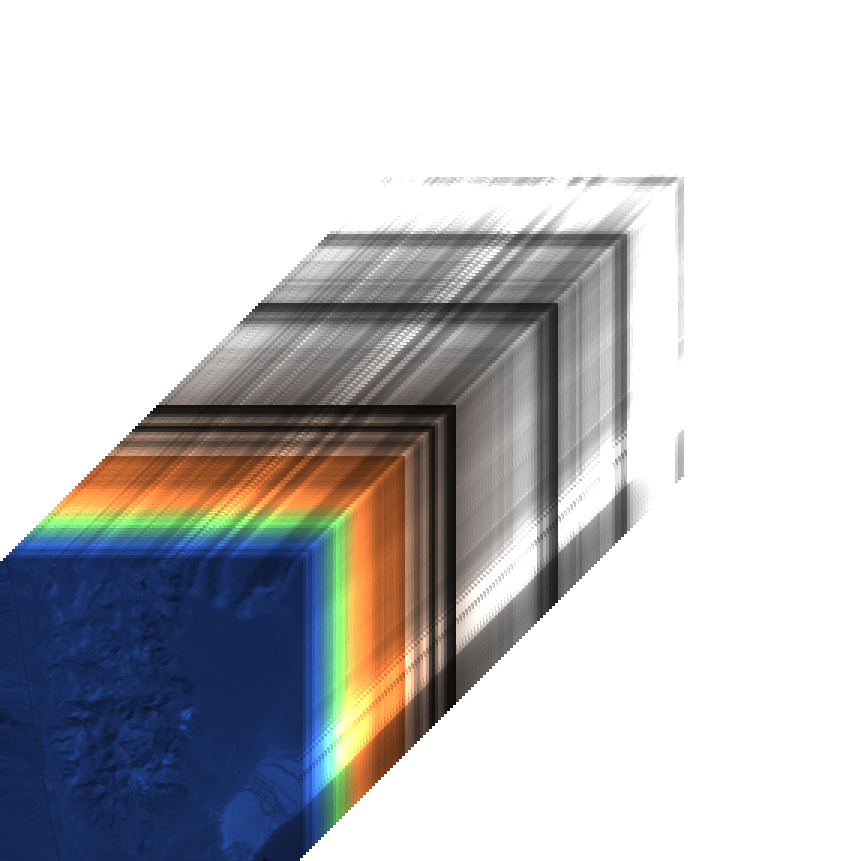
\includegraphics[width=8cm]{./fig/fig_01Intro/2D_HSI_Gen_copy/HSI}};
            \node at (nHSI)[xshift=  -5cm,yshift=-2.6cm](nm)  {\large $m$};
            \node at (nm)  [xshift= 0.7cm,yshift= 1.5cm](nmAr1) {$\;$} ;
            \node at (nm)  [xshift= 0.7cm,yshift=-1.5cm](nmAr2) {$\;$} ;
            \draw[<->] (nmAr1.-90) -- (nmAr2.90) ;
            \node at (nHSI)[xshift=-2.6cm,yshift=-4.5cm](nn)  {\large $n$} ;
            \node at (nn)  [xshift=-1.6cm,yshift= 0.2cm](nnAr1) {$\;$} ;
            \node at (nn)  [xshift= 1.6cm,yshift= 0.2cm](nnAr2) {$\;$} ;
            \draw[<->] (nnAr1.0) -- (nnAr2.180) ;
            \node at (nHSI)[xshift=-2.8cm,yshift= 1.0cm](nl)  {\large $\lambda$} ;
            \node at (nl)  [xshift=-1.5cm,yshift=-2.0cm](nlAr1) {$\;$} ;
            \node at (nl)  [xshift= 2.0cm,yshift= 1.5cm](nlAr2) {$\;$} ;
            \draw[<->] (nlAr1.45) -- (nlAr2.-135) ;
            \node at (0,0) [xshift=   1cm,yshift= 1.0cm](nRGB){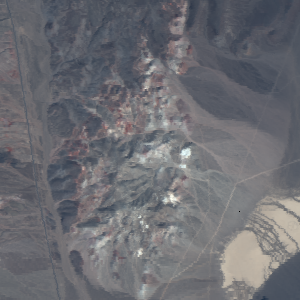
\includegraphics[width=2.5cm]{./fig/fig_01Intro/2D_HSI_Gen_copy/RGB}} ;
            \node at (nRGB)[xshift= 1.5cm,yshift=-3.0cm](nR)  {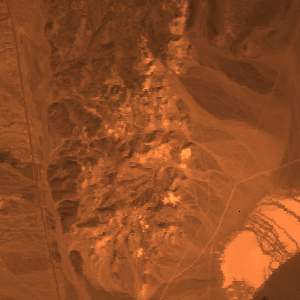
\includegraphics[width=2.5cm]{./fig/fig_01Intro/2D_HSI_Gen_copy/R}} ;
            \node at (nRGB)[xshift= 0.0cm,yshift=-3.5cm](nG)  {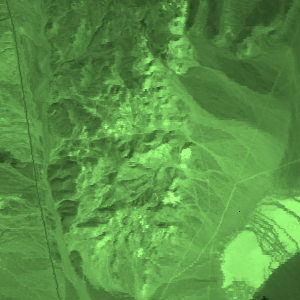
\includegraphics[width=2.5cm]{./fig/fig_01Intro/2D_HSI_Gen_copy/G}} ;
            \node at (nRGB)[xshift=-1.5cm,yshift=-4.0cm](nB)  {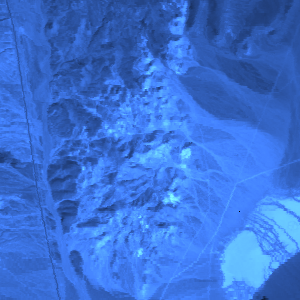
\includegraphics[width=2.5cm]{./fig/fig_01Intro/2D_HSI_Gen_copy/B}} ;
            \node at (nHSI)[xshift= 0.7cm,yshift=-3.5cm](nArr){$\;$} ;
            \node at (nArr)[xshift=-1.2cm,yshift=   0cm](nBAr1){$\;$} ;
            \node at (nArr)[xshift= 0.2cm,yshift=   0cm](nBAr2){$\;$} ;
            \node at (nArr)[xshift=-0.7cm,yshift= 0.2cm](nGAr1){$\;$} ;
            \node at (nArr)[xshift= 0.7cm,yshift= 0.2cm](nGAr2){$\;$} ;
            \node at (nArr)[xshift=-0.2cm,yshift= 0.4cm](nRAr1){$\;$} ;
            \node at (nArr)[xshift= 1.2cm,yshift= 0.4cm](nRAr2){$\;$} ;
            \draw          [blue ,->] (nBAr1.0) -- (nBAr2.180) ;
            \draw          [green,->] (nGAr1.0) -- (nGAr2.180) ;
            \draw          [red  ,->] (nRAr1.0) -- (nRAr2.180) ;
            \draw          [decorate,
                            decoration={brace,amplitude=10pt},
                            xshift=   1cm,yshift=-0.7cm]
                            (-2.7,0.0) -- (2.7,0.0) ;
        \end{tikzpicture}
    }
    \caption{HSI over an Earth surface and its conversion to ordinary color image.}
    \label{fig:INTRO_HSI}
\end{figure}

Hyperspectral unmixing and classification belong to a class of quantitative
analysis techniques that retrieve useful information from the pixels of HSIs.
These analysis have great potential in applications where the image scenes
tend to be large and complex, such as remote sensing, Earth science,
industrial resource exploration, aircraft-based systems, agricultural science
and wide area monitoring, or in small scale laboratory-based studies like food
quality analysis, chemical spectroscopy, biomedical science and forensic
science
\cite{IMG_SPECTROMETRY_FOR_EARTH_REMOTE_SENSING,
      ADV_IN_HS_REMOTE_SENSING_FOR_GEO_MAP,
      A_REVIEW_ON_APPL_OF_NIR_SPECTRO_AND_CHEM_FOR_AGROFOOD_PROC_INDST,
      HSI_FOR_FOOD_APPL,
      APPL_OF_ICA_WITH_JADE_ALGO_AND_NIR_HSI_FOR_REVEALING_FOOD_ADULTERATION},
to mention a few.
Usually an enhancement in the quality of an HSI in terms of spatial and
spectral resolution is beneficial to all hyperspectral imagery applications.
% identification, classification, mapping and unmixing.
In this thesis, the enhancement of HSIs in spatial and spectral quailty,
called hyperspectral super-resolution (HSR), for remote sensing purpose is
discussed.

\section{Overview of the Hyperspectral Super-resolution (HSR)}
\label{sec:HSR}
In geoscience and Earth science research, a number of industries have launched
satellites for Earth observation missions.
These projects include Sentinel, Landsat, RapidEye, QuickBird, EnMAP, AVIRIS,
HYPXIM, CHRIS, HISUI, Hyperion, DESIS, PRISMA, SHALOM, etc.
The resolution characteristics of the aforementioned wide spectrum of remote
sensing instruments are summarized in Figure \ref{fig:INTRO_HSMSSensors_Res}
\cite{HSMS_DATA_FUSION_A_COMPARATIVE_REVIEW}
in which more desirable sensors characteristics are marked in the purple
region; the hyperspectral (HS) and multispectral (MS) sensors are marked by
the blue dots and red dots, respectively.
From the figure we see that an ideal hyperspectral sensor should have small
GSD and large amount of spectral bands within a desired wavelength range.
However, in practice, hyperspectral sensors with such high spatial and
spectral resolution are not common due to hardward limitation, \ie we are
inevitably required to have a trade-off between the two resolutions.
\begin{figure}[t]
    \centering
    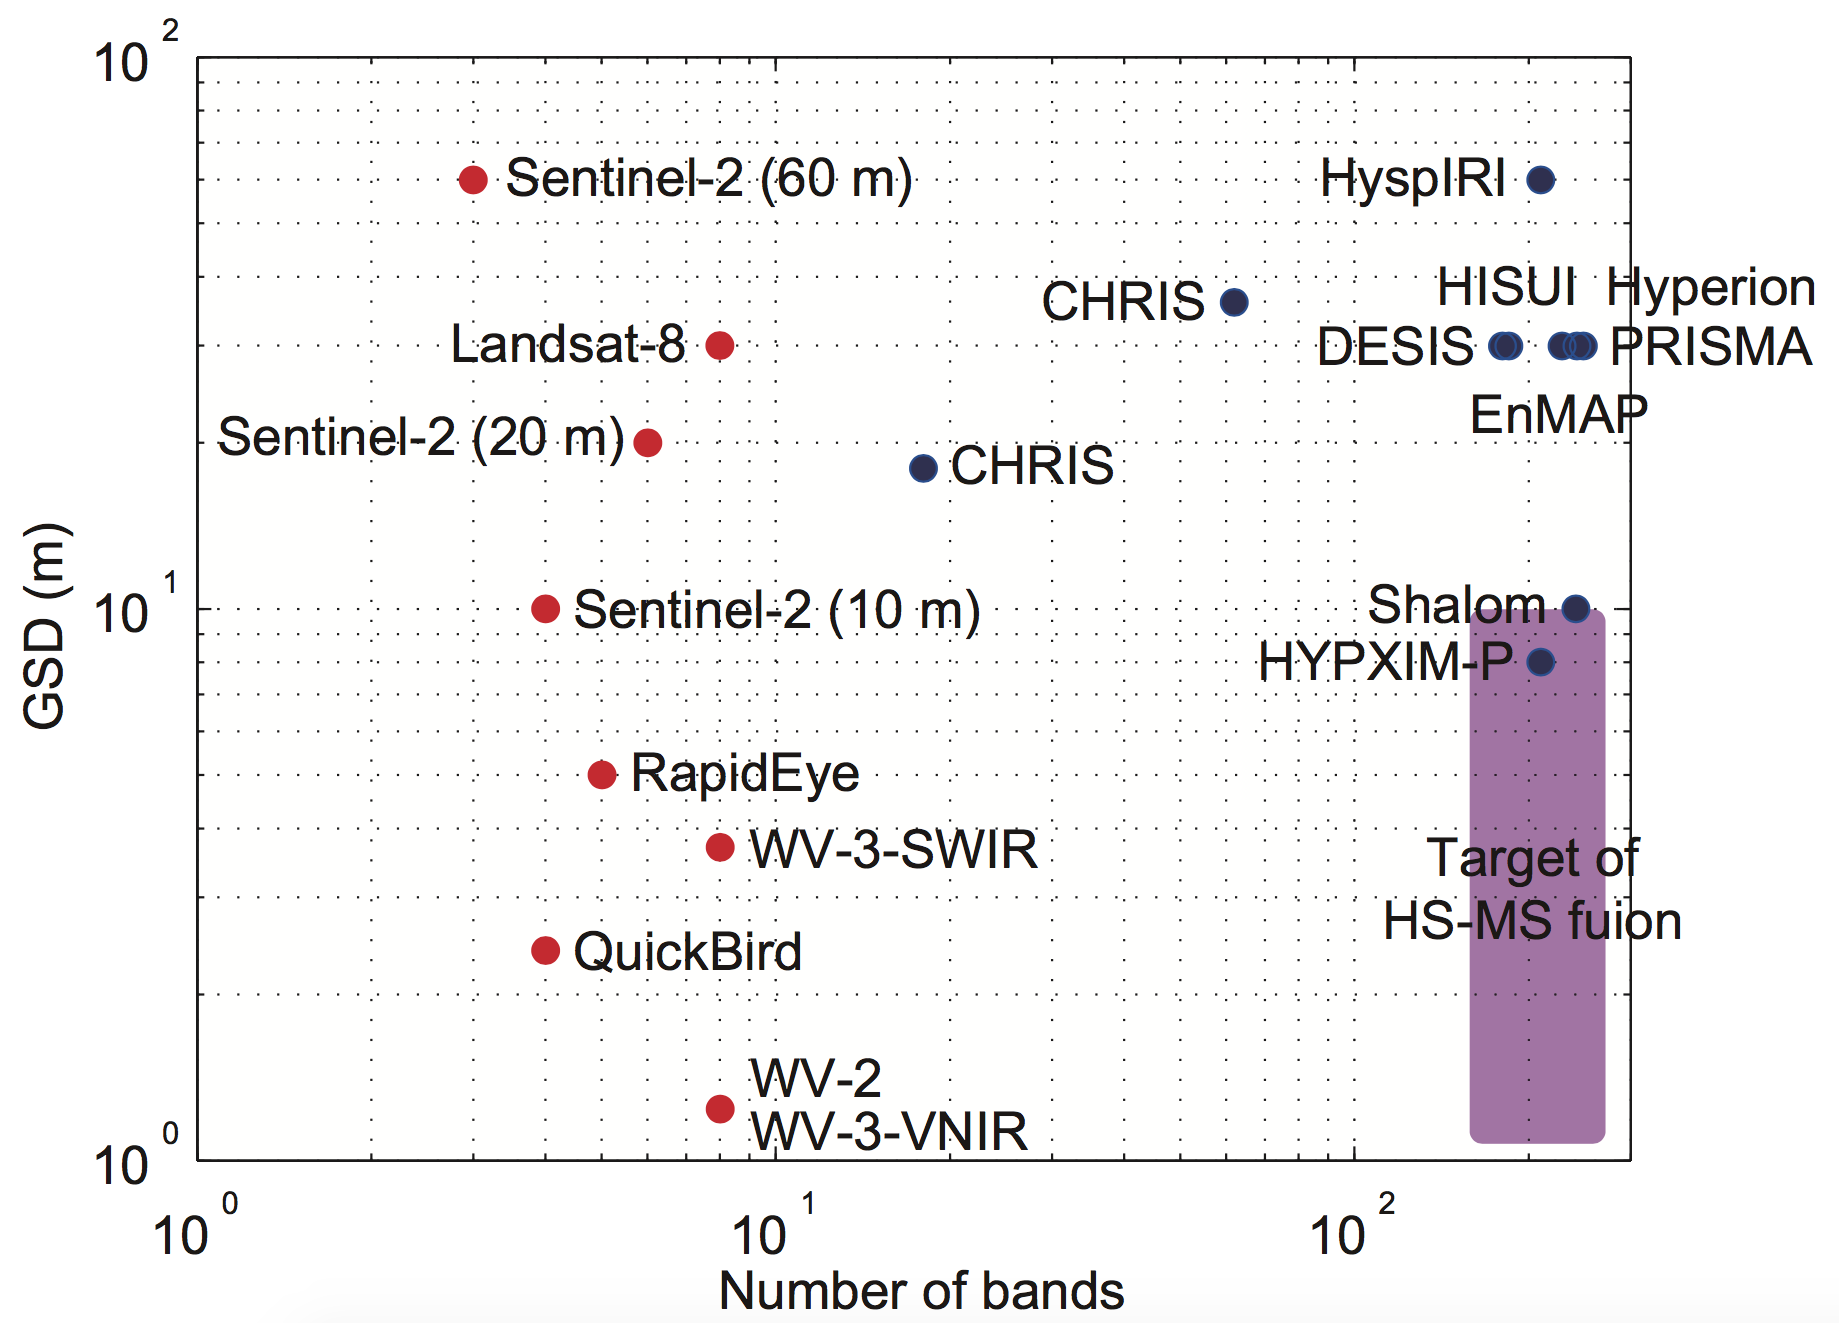
\includegraphics[width=.75\textwidth]{./fig/fig_01Intro/Introduction_HSMSSensors_Res}
    \caption{Resolutions of the latest remote satellite sensors
             \cite{HSMS_DATA_FUSION_A_COMPARATIVE_REVIEW}.}
    \label{fig:INTRO_HSMSSensors_Res}
\end{figure}

In this thesis, for ease of presentation, we define images with high
spectral resolution and low spatial resolution as hyperspectral (HS) images;
images with low spectral resolution and high spatial resolution as
multispectral (MS) images; images with high resolution in both spatial and
spectral domain as super-resolution (SR) images.
HSR estimates the SR image of a scene from its HS and MS observations such
that the combined image at most possesses the spectral resolution of the
former and spatial resolution of the latter (Figure \ref{fig:fusion_flow}).
\begin{figure}[t]
    \centering
    \resizebox{0.98\linewidth}{!}{
        \begin{tikzpicture}
            [dot/.style={circle,draw=black,fill=white,inner sep=5pt,minimum size=5pt}]
            \node at (0,0) [dot,draw=black,very thick ](n+)  {\Huge +};
            \node at (n+)  [xshift= -5cm,yshift=   3cm](nHS) {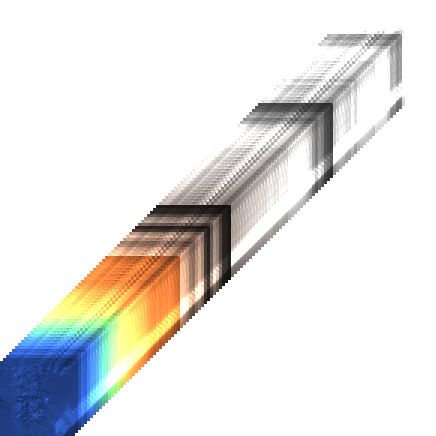
\includegraphics[width=5cm]{./fig/fig_01Intro/2D_HSI_Gen_copy/HS} };
            \node at (n+)  [xshift= -5cm,yshift=  -3cm](nMS) {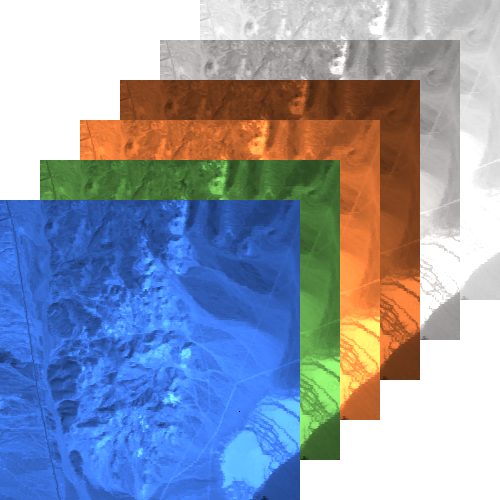
\includegraphics[width=5cm]{./fig/fig_01Intro/2D_HSI_Gen_copy/MS} };
            \node at (n+)  [xshift=  7cm,yshift=   0cm](nHSI){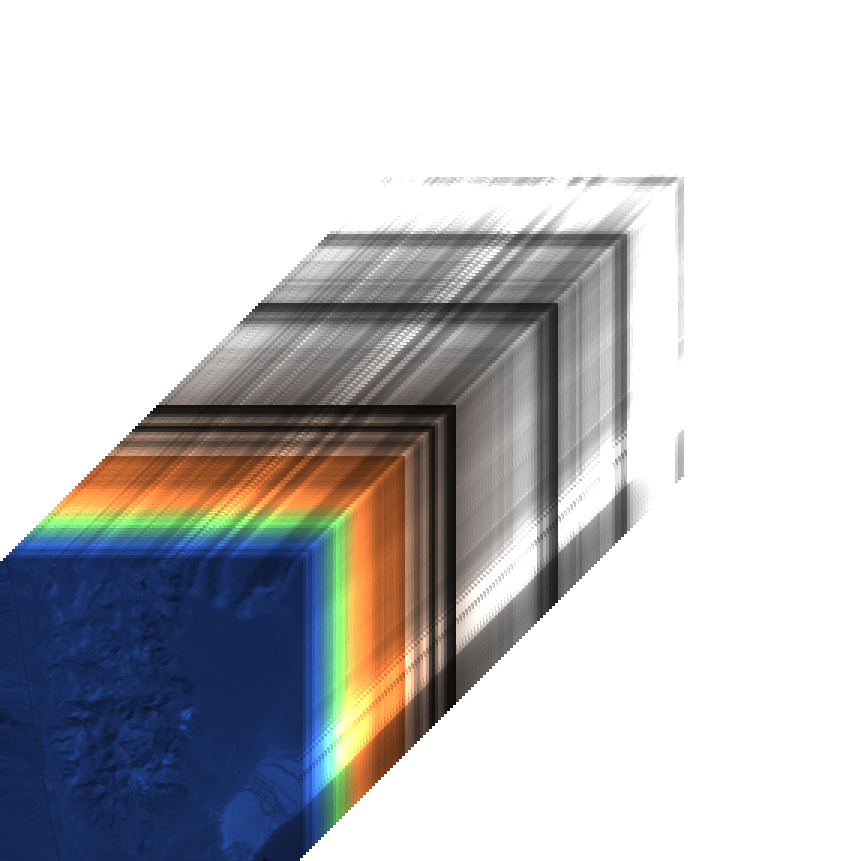
\includegraphics[width=8cm]{./fig/fig_01Intro/2D_HSI_Gen_copy/HSI}};
            \node at (n+)  [xshift=1.4cm,yshift= 1.2cm]      {\Large HSR                             };
            \node at (nHS) [xshift=  1cm,yshift=-1.5cm]      {\Large HS Image                        };
            \node at (nMS) [xshift=  1cm,yshift= 3.2cm]      {\Large MS Image                        };
            \node at (nHSI)[xshift=  1cm,yshift= 3.0cm]      {\Large SR Image                        };
            \draw[-{>[scale=2.5,length=5,width=6]},line width=1.2] (nHS.-30) -- (n+.140);
            \draw[-{>[scale=2.5,length=5,width=6]},line width=1.2] (nMS.30)  -- (n+.220);
            \draw[-{>[scale=2.5,length=5,width=6]},line width=1.2] (n+.0)  -- (nHSI.180);
        \end{tikzpicture}
    }
    \caption{Hyperspectral super-resolution from low resolution HS and MS images.}
    \label{fig:fusion_flow}
\end{figure}
Many approaches have been studied including Component Substitution (CS)
\cite{HSMSEXISTAPPROACH_CS_IHS,
      HSMSEXISTAPPROACH_CS_ENHANCING_MS_BY_PAN,
      HSMSEXISTAPPROACH_CS_IMPROVE_CS},
Multiresolution Analysis (MRA)
\cite{HSMSEXISTAPPROACH_MRA_SMOOTH_FILTER_IMG_FUSION,
      HSMSEXISTAPPROACH_MRA_MTF},
Bayesian approach
\cite{HSMSEXISTAPPROACH_BAYESIAN_STOC_MIX_MODEL_HSR,
      HSMSEXISTAPPROACH_BAYESIAN_MAP_ESTIMATE_HSR,
      HSMSEXISTAPPROACH_BAYESIAN_HSR_BY_MS}
and spectral unmixing
\cite{CNMF,
      HSMSEXISTAPPROACH_MF_NMFPAN,
      HSR_MF,
      HSMSEXISTAPPROACH_MF_SPAT_SPEC_IMG_FUSION,
      HSMSEXISTAPPROACH_MF_HSR_LOCAL_LOWRANK,
      HSMSEXISTAPPROACH_MF_JOINT_HSR_UNMIX_INTERACT_FEEDBACK}.
The competitiveness of these classes of methods have been summarized and
reviewed in
\cite{HS_PANSHARPENING_A_REVIEW,HSMS_DATA_FUSION_A_COMPARATIVE_REVIEW}.
In this thesis, we focus on HSR by spectral unmixing.

\section{Overview of Convex Optimization}
Some basic concepts of convex optimization are reviewed in this section.
First of all, a few definitions on convex sets and convex functions are
given before further discussion on convex optimization problems.

\subsection{Convex Sets}
A set $\mathcal S \subseteq \R^N$ is convex if the line segment drawn from any
two points in $\mathcal S$ lies in $\mathcal S$, \ie
$\forall \; \bm x,\bm y \in \mathcal S$,
\begin{equation}
    \alpha \bm x + (1-\alpha) \bm y \in \mathcal S, \;\;\;
    \forall \; \alpha\in[0,1].
\end{equation}
Some examples of convex sets are given as
\begin{itemize}
    \item $\R^n_+$ (nonnegative orthant);
    \item $\{\bm x \in \R^2_+ \;|\; x_1 - 3x_2 \leq 0, -2x_1 + 3x_2 \leq 0\}$
          (a convex cone);
    \item $\{\bm x \in \R^n \;|\; \Vert \bm x \Vert_2 \leq 1\}$ (unit $\ell_2$-norm ball);
    \item $\{\bm x \in \R^n \;|\; \Vert \bm x \Vert_1 \leq 1\}$ (unit $\ell_1$-norm ball);
    \item $\{\bm x \in \R^n \;|\; \vert x_i \vert \leq 1\}$ (a box).
\end{itemize}

\subsection{Convex Functions}
A function $f:\mathcal S\rightarrow\R$ is said to be convex if $\mathcal S$ is
a convex set and $f$ satisfies
\begin{equation}
    f(\alpha \bm x + (1-\alpha) \bm y) \leq
    \alpha f(\bm x) + (1-\alpha) f(\bm y), \;\;\;
    \forall \; \bm x \; , \; \bm y \in \R^N \; , \; \alpha \in [0,1].
    \label{eq:convex_function_definition_1}
\end{equation}
If $f(\bm x)$ is differentiable in $\bm x$ within $\mathcal S$, then the
condition in \eqref{eq:convex_function_definition_1} is equivalent to
\begin{equation}
    f(\bm y) \geq f(\bm x) + \nabla f(\bm x)\Tr (\bm y - \bm x),
    \label{eq:first_order_condition}
\end{equation}
where $\nabla f(\bm x)$ denotes the gradient of $f$ at point $\bm x$.
\eqref{eq:first_order_condition} is called the first order condition in the
literature.

\subsection{Convex Optimization Problems}
Consider the following optimization problem.
\begin{equation}
    \begin{array}{cl}
        \underset{\bm x}{\min} & f(\bm x) \\
        \text{s.t.}            & \bm x \in \mathcal S,
    \end{array}
    \label{eq:general_convex_optimization_problem}
\end{equation}
where $\bm x$ is the decision variable, $f$ is the objective function in
$\bm x$ and $\mathcal S$ is the feasible set of $\bm x$.
If function $f$ and feasible set $\mathcal S$ of
\eqref{eq:general_convex_optimization_problem} are both convex, then
\eqref{eq:general_convex_optimization_problem} is called a convex optimization
problem.
A convex optimization problem has the following properties:
\begin{itemize}
    \item [1)] Any locally optimal points are globally optimal;
    \item [2)] If $f$ is differentiable everywhere in $\mathcal S$, then the
               first-order condition holds;
    \item [3)] If $\bm x^* \in \mathcal S$ is a minimizer of problem
               \eqref{eq:general_convex_optimization_problem}, then
               \begin{equation}
                   \nabla f(\bm x^*)\Tr (\bm y - \bm x^*) \geq 0
                   \;\;\; \forall \; \bm y \in \mathcal S.
               \end{equation}
\end{itemize}

\section{Significance of Convex Optimization}
%Convex optimization problems can be solved easily and efficiently.
If a real world problem can be formulated as a convex optimization problem,
then in general this problem can be solved exactly, efficiently and easily by
methods like first order gradient method (FOGM), interior point method and
many more.
History has shown that convex optimization has been benefitting many practical
situations including automatic control
systems, signal estimation and detection, communications, network design and
data modelling while there are abundant reliable computer software that help
solve their problems.


\section{Coordinate Descent Algorithms}
A coordinate descent algorithm solves optimization problems by successively
performing approximate minimization along coordinate directions (or coordinate
hyperplanes)
\cite{COORD_DESCENT_ALGO}.
It is an iterative method in which each iterate is obtained by fixing most
components of the decision variable vector $\bm x$ at their values from the
current iteration, and approximately minimizing the objective with respect to
the remaining components.
Typically, this approach lowers the dimensions of the subproblems and thus
motivates people solving the subproblems and updating the variables in an
easier and more efficient way compared with handling the full problem and the
full variable vector.

Specifically, consider the decision variable $\bm x \in \mathcal X$ that is
decomposable into $N$ blocks as $\bm x \coloneqq (\bm x_1,\cdots,\bm x_N)$;
$\mathcal X \coloneqq \mathcal X_1 \times \cdots \mathcal X_N$ as the feasible
set; $f:\mathcal X \rightarrow \R$ as the objective function that can be
expressed as $f(\bm x_1,\cdots,\bm x_N)$; the function that depends on
$\bm x_i$ as $f_i(\bm x_1,\cdots,\bm x_i,\cdots,\bm x_N)$.
A general optimization problem of the form
\begin{equation}
    \begin{array}{cl}
        \underset{\bm x}{\min} & f(\bm x) \\
        \text{s.t.}            & \bm x \in \mathcal X
    \end{array}
\end{equation}
can be solved to a stationary point by a coordinate descent algorithm
described below.
\begin{algorithm}
    \caption{Coordinate Descent Algorithm}
    \label{alg:CD}
    \begin{algorithmic}[1]
        \Require{$\bm x\iter{0} \in \mathcal{X}$.}
        \For{$k=1,2,\cdots$ until stopping criteria holds}
            \State{$\bm x\iter{k,0} \gets \bm x\iter{k}$.}
            \For{$i=1,\cdots,N$}
                \State{Update:
                       \begin{equation}
                           \bm x_i\iter{k,i}
                           \gets
                           \begin{cases}
                               \underset{\bm x_j \in \mathcal X_i}{\min}
                               f_i(\bm x_1    \iter{k,i  },\cdots,
                                   \bm x_{j-1}\iter{k,i  },
                                   \bm x_j                ,
                                   \bm x_{j+1}\iter{k,i-1},\cdots,
                                   \bm x_N    \iter{k,i-1})
                               & j = i, \\
                               x_j\iter{k,i-1}
                               & j\neq i.
                           \end{cases}
                       \end{equation}
                      }
            \EndFor
            \State{$\bm x\iter{k+1} \gets \bm x\iter{k,i}$.}
        \EndFor
        \Ensure{$\bm x\iter{k+1}$.}
    \end{algorithmic}
\end{algorithm}

At the $k\thtxt$ iteration, the above CD algorithm separates the full problem
$\underset{\bm x\in\mathcal X}{\min}\;f(\bm x)$ into $N$ subproblems which
approximate $f$ along each coordinate direction at the current state
$x\iter{k}$.
The algorithm then exactly solves each subproblem in a cyclic sense.
Note that the variable update is not necessarily ordered in a cyclic manner.
It could be a randomized sequence between $1$ and $N$ or an order following
the coordinate index whose gradient component has the maximal absolute value,
as illustrated in
\cite{NESTEROV_BCD_HUGE_PROBLEM}.

CD algorithm can be easily extended to a Block-CD (BCD) algorithm by each time
considering the decision variable vector $\bm x$ along multiple coordinate
directions (or coordinate hyperplanes).
Examples of BCD benefitting a wide range of applications can be found in
\cite{BCD_APPL_STAT_TOMOGRAPHY,
      BCD_APPL_DIFF_TOMOGRAPHY,
      BCD_APPL_BCD_FOR_MULTITASK_LASSO_NEURAL_DISCOV,
      BCD_APPL_PROTEIN_LOOP,
      BCD_APPL_OD_MATRIX_ADJ_PROBL,
      BCD_APPL_BIOFEATURE,
      BCD_APPL_SPARSE_COV_EST,
      BCD_APPL_LARGESCALE_LINEAR_SVM}.

\section{Contributions}
In this thesis we investigate the efficiency and effectiveness of BCD using
FOGMs to tackle the HSR problem.
Specifically, the non-convex HSR problem is separable into two block convex
subproblems that can be individually solved by FOGMs.
We study the effect of exactness of solving the subproblems towards the full
HSR performance in terms of accuracy and runtime.
We find that with inexact solving of the subproblems (\ie inexact BCD), the
HSR can still be solved to a stationary point while the accuracy can be
preserved and, more importantly, the runtime is largely reduced compared to
state-of-the-art algorithms.
%The importance of the 
%The study goes through two state-of-the-art problem formulations.
%The contributions is that a fast framework of FOGMs is proposed with the
%benefit being that the computation time required is much less than that
%required by the state of the arts while a comparable HSR quality is achieved.

\section{Organization}
The organization of this thesis is as follows.
Chapter 2 describes the system model and the HSR problem.
Chapter 3 describes how FOGMs may solve a quadratic program in detail.
After that the HSR problem is shown to be a two block quadratic program that
can be handled by BCD algorithms.
Chapter 4 presents synthetic and semi-real simulations to compare the
performance by BCD algorithms using FOGMs and that by state-of-the-art
algorithms.
Chapter 5 summarizes this thesis.

 % Introduction
\chapter{The HSR Problem and The State-of-the-art Algorithms}

This chapter describes the HSR problem in detail.
The organization of this chapter is as follows.
First the HS and MS sensor characteristics are discussed, followed by the
signal model that simulates their characteristics are developed.
Then we described the commonly used signal model for hyperspectral images
named "Linear Mixing Model" (LMM).
Finally the HSR problem statement is presented.

%The HSR problem statement is a hyperspectral unmixing (HU) based MF problem
%that finds an estimate of the underlying endmember signatures and
%their corresponding abundance, which constitute the desired SR image, from
%the HS and MS image pair.

\section{Signal Model of HS and MS Sensors}
Let $\bm{\mathcal Y} \in \R_+^{\ell_1 \times \ell_2 \times M}$ be a
nonnegative tensor representing the pixel values of an SR image with
$L = \ell_1 \cdot \ell_2$ pixels and with $M$ spectral bands.
The tensor $\bm{\mathcal Y}$ can be lexicographically unfolded to a
nonnegative matrix $\bm Y \in \R_+^{M \times L}$.
The column-wise view and row-wise view of $\bm Y$ are shown in
\eqref{eq:col_view_Y} and \eqref{eq:row_view_Y}, respectively, such that
$\{\bm y_i\}_{i=1}^L \in \R_+^M$ represents the spectral reflectance signature
at the $i\thtxt$ pixel and $\{\bm y^j\}_{j=1}^M \in \R_+^L$ represents the
%vectorized abundance fraction map of all endmembers at the $j\thtxt$
vectorized reflectance map of the SR image at the $j\thtxt$
spectral band.
Figure \ref{fig:HSI_unfolding} illustrates the process of unfolding a spectral
image from a tensor to a matrix.
\begin{eqnarray}
    \bm Y & = & \begin{bmatrix} \bm y_1 & \bm y_2 & \cdots & \bm y_L \end{bmatrix} \label{eq:col_view_Y} \\
    \bm Y & = & \begin{bmatrix} \bm y^1 & \bm y^2 & \cdots & \bm y^M \end{bmatrix}^\text T
    \label{eq:row_view_Y}
\end{eqnarray}

\begin{figure}[t]
    \centering
    \resizebox{0.85\linewidth}{!}{
        \begin{tikzpicture}
            \node at (0,0)   [xshift=   0cm,yshift=   0cm]                                (center) {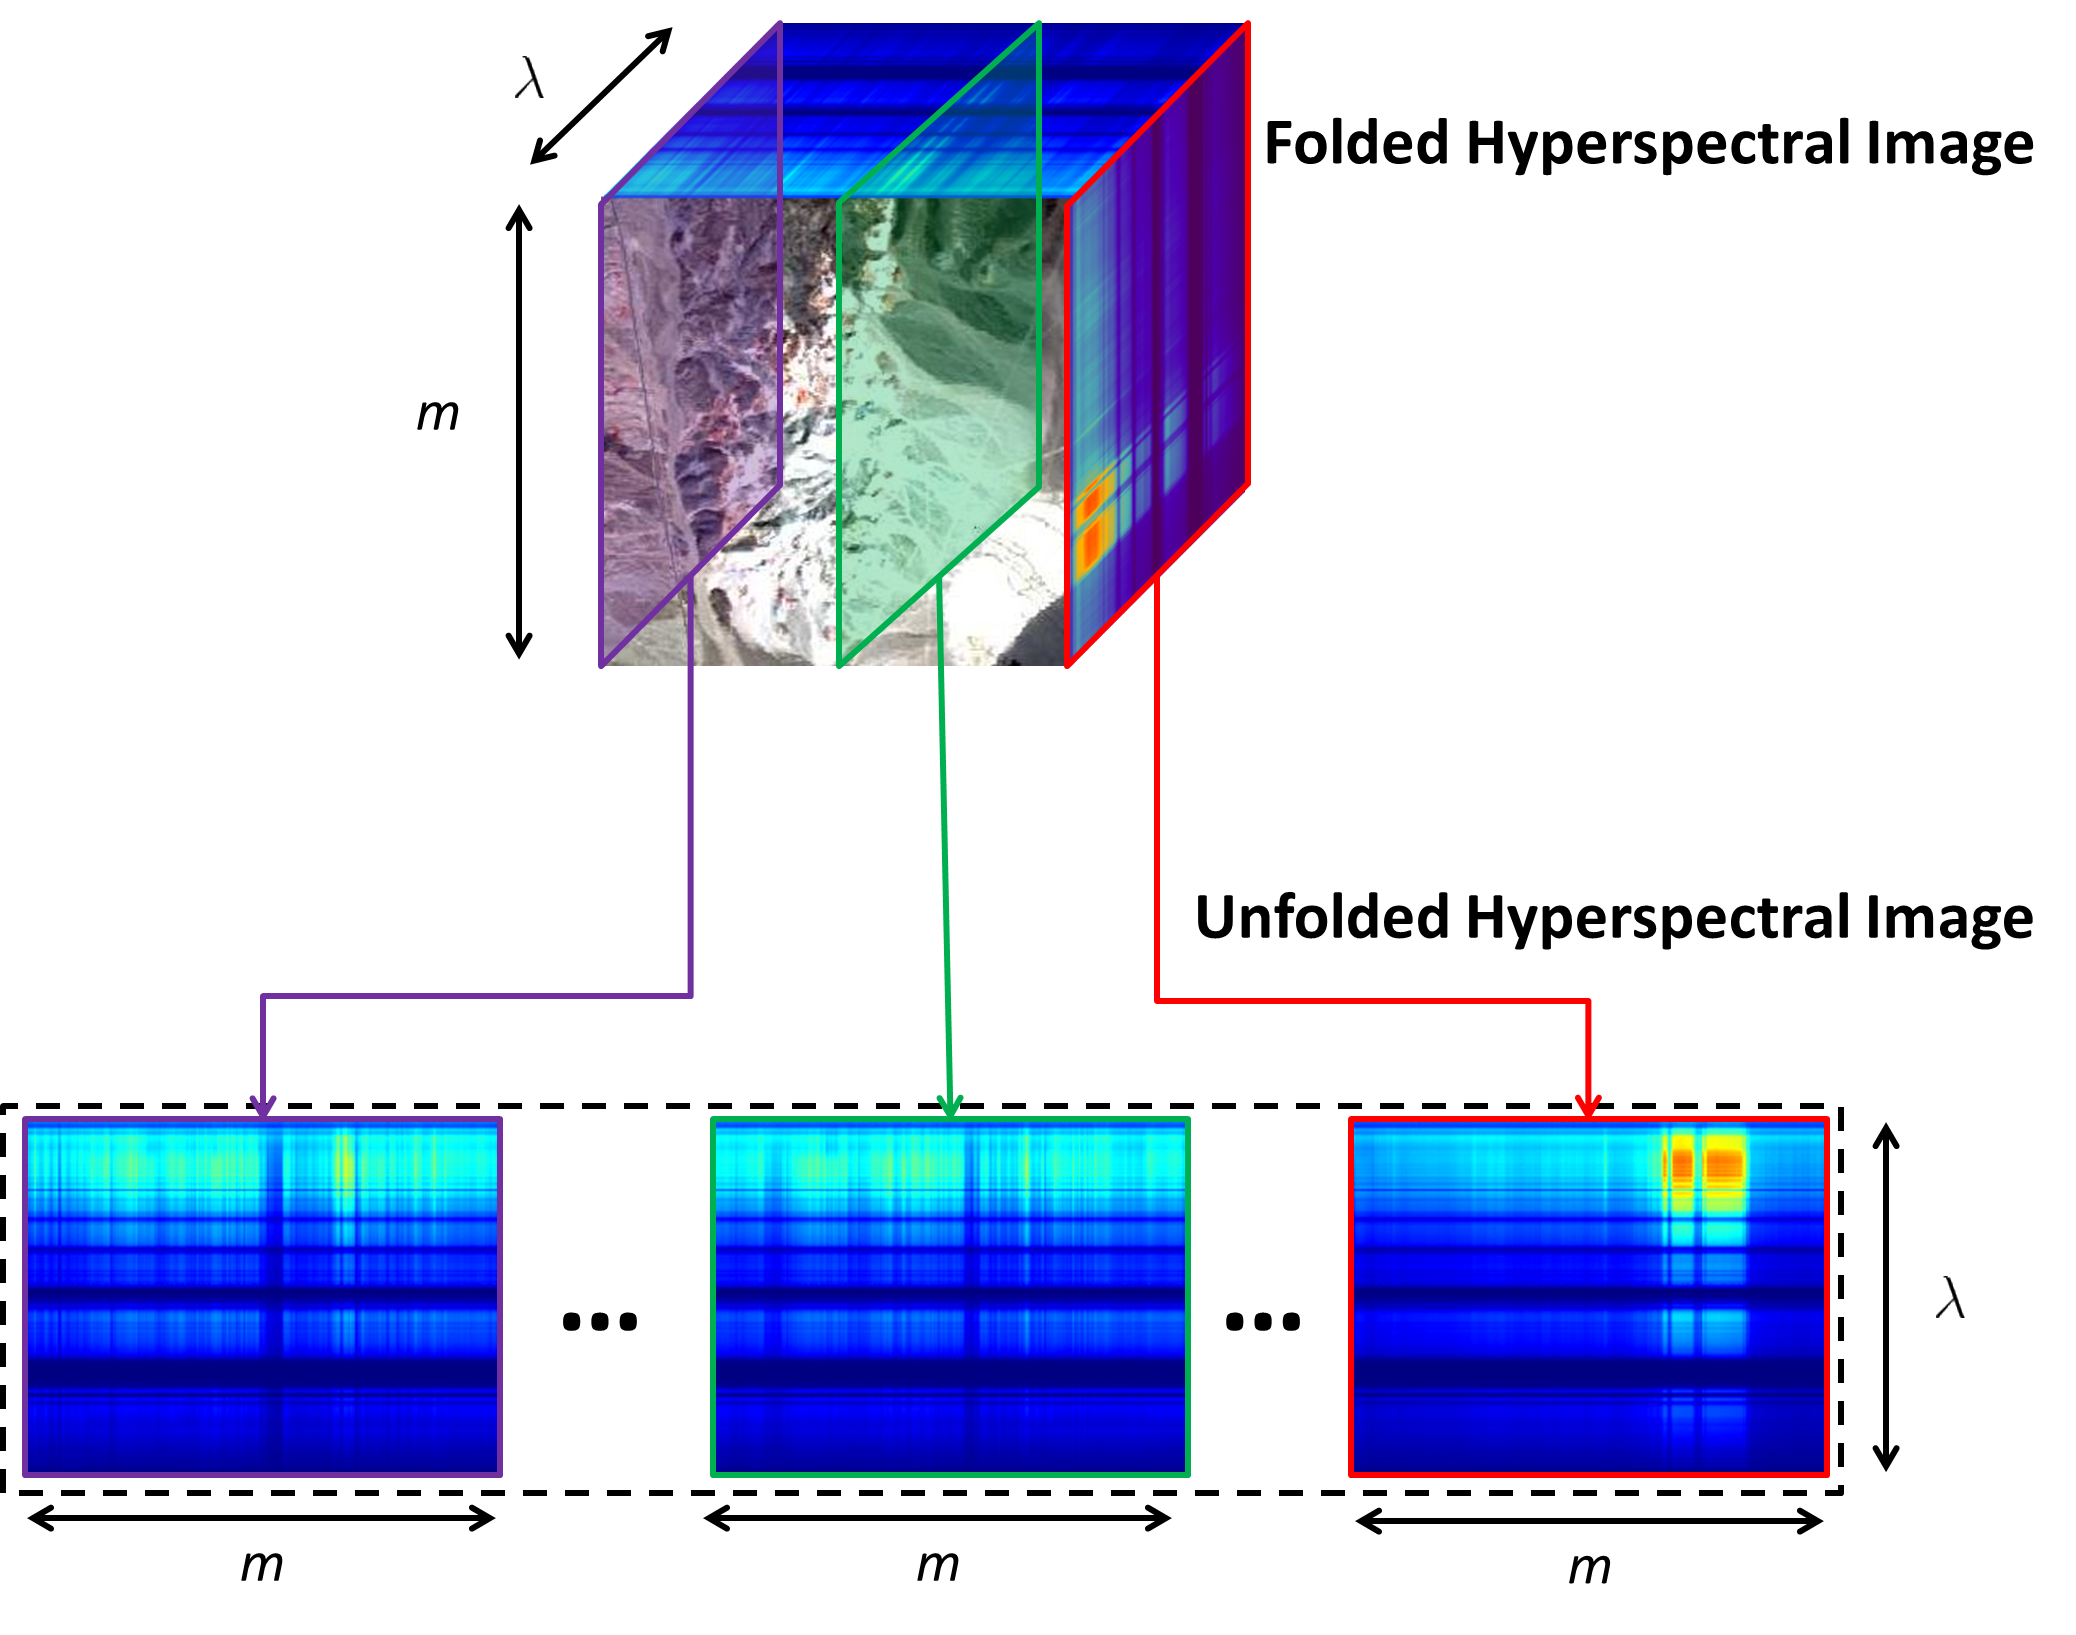
\includegraphics[width=0.8\columnwidth]{./fig/fig_02HSR_Problem/HSR_Problem_HSI_unfolding}} ;
            \node at (center)[xshift= 3.9cm,yshift= 3.8cm,text width=5cm  ,fill=white!20]          {Folded Hyperspectral Image};
            \node at (center)[xshift= 3.9cm,yshift=-0.5cm,text width=6cm  ,fill=white!20]          {Unfolded Hyperspectral Image};
            \node at (center)[xshift=-3.5cm,yshift= 2.2cm,text width=0.5cm,fill=white!20]          {$\ell_1$};
            \node at (center)[xshift=-4.3cm,yshift=-4.4cm,text width=0.5cm,fill=white!20] (t1)     {$\ell_1$};
            \node at (t1)    [xshift= 3.8cm,yshift=   0cm,text width=0.5cm,fill=white!20] (t2)     {$\ell_1$};
            \node at (t2)    [xshift= 3.8cm,yshift=   0cm,text width=0.5cm,fill=white!20]          {$\ell_1$};
            \node at (center)[xshift=-3.1cm,yshift= 4.1cm,text width=0.5cm,fill=white!20]          {$M$};
            \node at (center)[xshift= 5.3cm,yshift=-2.8cm,text width=0.5cm,fill=white!20]          {$M$};
        \end{tikzpicture}
    }
    \caption{Unfolding a hyperspectral image from a tensor to a matrix.}
    \label{fig:HSI_unfolding}
\end{figure}

In the signal model an SR image is partially observed by an HS sensor and by
an MS sensor.
Let $\YH\in\R_+^{M \times L_\text H}$ and $\YM\in\R_+^{M_\text M \times L}$
represent the vectorized observed HS and MS images, respectively, where
$L_\text H$ is the number of pixels of the HS image and $M_\text M$ is the
number of spectral bands of the MS image.
As introduced in Section \ref{sec:HSR}, we know that HS images have higher
spectral resolution and MS images have higher spatial resolution so that the
following inequality hold:
\begin{eqnarray}
    M         & > & M_\text M, \\
    L_\text H & < & L.
\end{eqnarray}
\begin{figure}[t]
    \centering
    \subfigure[$\;$]{\label{fig:IMG_DOWNSAMP_full400x400}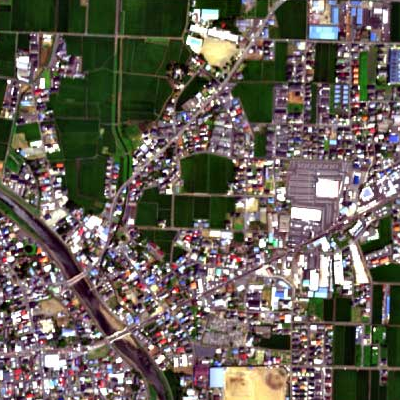
\includegraphics[width=0.3\columnwidth]{./fig/fig_02HSR_Problem/IMG_DOWNSAMP_full400x400}}
    \subfigure[$\;$]{\label{fig:IMG_DOWNSAMP_blur400x400}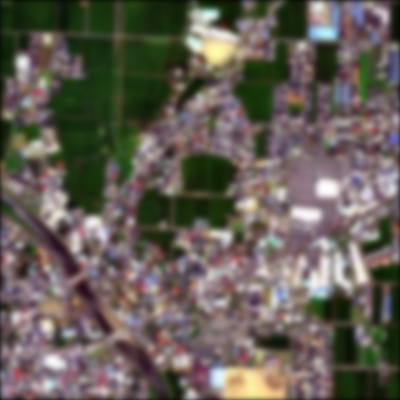
\includegraphics[width=0.3\columnwidth]{./fig/fig_02HSR_Problem/IMG_DOWNSAMP_blur400x400}}
    \subfigure[$\;$]{\label{fig:IMG_DOWNSAMP_down50x50}  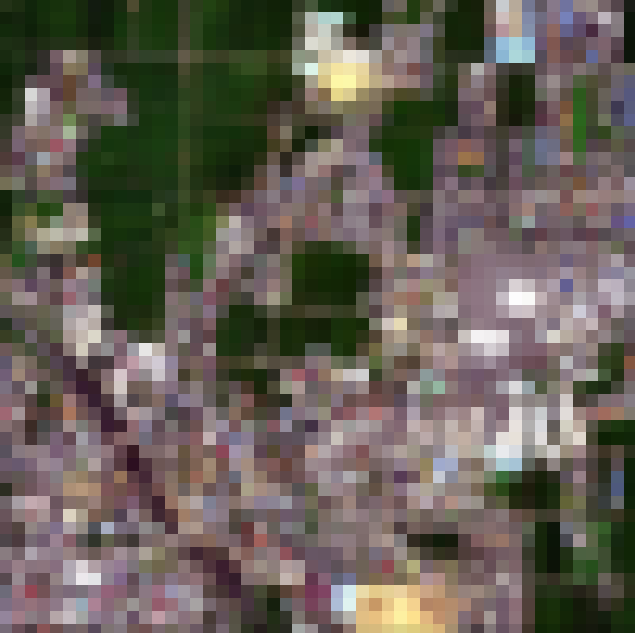
\includegraphics[width=0.3\columnwidth]{./fig/fig_02HSR_Problem/IMG_DOWNSAMP_down50x50}  }
    \caption{Effect of spatial degradation by HS sensors:
             (a) High spatial resolution image with $400 \times 400$ pixels;
             (b) Image of (a) blurred by a $25 \times 25$ Gaussian filter of
                 variance $\sigma = 3$;
             (c) Image of (b) subsampled on every $8$ pixels vertically and
                 horizontally.}
    \label{fig:IMG_DOWNSAMP_down80x80}
\end{figure}

\subsection{Spatial Degradation Model in HS Sensors}\label{sec:SPATIAL_DOWNSAMPL_MODEL}
An HS sensor degrades the spatial contents of SR images.
The relation between $\bm Y$ and $\YH$ can be modelled as
\begin{equation}
    \YH = \bm Y \bm G + \bm V_\text H,
    \label{eq:spatial_degradation_model}
\end{equation}
where $\bm G \in \R^{L \times L_\text H}$ is a matrix representing the spatial
degradation effect that may be composed of geometric wrapping, translation,
blurring and subsampling operations and $\bm V_\text H$ represents the noise
in the HS sensor.
Note that $\bm G$ is a matrix multiplied to the vectorized reflectance maps of
each band $\{(\bm y^j)\Tr\}_{j=1}^N$.
In this thesis the spatial responses considered include blurring and
subsampling operations.
Therefore, $\bm G$ can be expressed as
\begin{equation}
    \bm G = \bm B \bm D,
    \label{eq:spatial_degradation_model_G}
\end{equation}
where the multiplication with $\bm B \in \R^{L \times L}$ and
$\bm D \in \R^{L \times L_\text H}$ represents two different stages of spatial
responses.
The first stage is a spatial low-pass filtering where the $\ell\thtxt$ column
of $\bm B$ is a vectorized point spread function applied onto the $\ell\thtxt$
pixel of $\bm Y$.
Typically $\bm B = [\bm b_1 \cdots \bm b_L]$ is a convolution matrix of a two
dimensional normalized low-pass filter kernel.
The second stage is a spatial subsampling process with
$\bm D \in \{0,1\}^{L \times L_\text H}$ being a subsampling matrix that draws
the reflectance maps $\{(\bm y^j)\Tr\}_{j=1}^M$ vertically and horizontally on
every $d$ pixels, where $d = \sqrt{L/L_\text H}$ is the downsampling
factor.
Figure \ref{fig:IMG_DOWNSAMP_down80x80} illustrates a standard high spatial
resolution color image (a), passing through a spatial low-pass filter
(b), and then further passing through a subsampling response (c).

\subsection{Spectral Degradation Model in MS Sensors}\label{sec:SPECTRAL_DOWNSAMPL_MODEL}
An MS sensor undersamples the SR images in spectral domain by receiving signals
at fewer but wider spectral range, resulting in MS images having only few
broad band images.
The matrices $\bm Y$ and $\YM$ can be related by
\begin{equation}
    \YM = \bm F \bm Y + \bm V_\text M,
    \label{eq:spectral_degradation_model}
\end{equation}
where $\bm F \in \R_+^{M_\text M \times M}$ represents the spectral degradation
matrix of the MS sensor system; $\bm V_\text M$ is the noise in the MS sensor.

To better illustrate the spectral response of HS and MS sensors, we take an
airborne hyperspectral sensor named "AVIRIS" and a satellite multispectral
sensor named "Thematic Mapper (TM) Sensor" as examples.
They have been serving as the core instruments of NASA's Earth monitoring
projects for many years since mid 80s.
The AVIRIS sensor, as introduced in Chapter 1, observes the Earth surface at
$224$ spectral bands covering wavelengths between $0.4\,\mu$m and $2.5\,\mu$m
at norminally $10\,$nm intervals.
The TM sensor, on the other hand, observes the Earth surface at fewer spectral
bands with a wider interval.
Among them, six of which overlap with the spectral range of the AVIRIS sensor
($0.4\,\mu$m-$2.5\,\mu$m).
The spectral response of the TM sensor is shown in Figure
\ref{fig:LANDSAT7_TM_RSR}
\cite{LANDSAT_SPECTRAL_RESPONSE,
      LANDSAT_HANDBOOK,
      SPECTRAL_RESPONSE_OF_LANDSAT8}.
\begin{figure}[t]
    \centering
    \resizebox{0.98\linewidth}{!}{
        \begin{tikzpicture}
            % HS Matrix
            \node at (0,0) [xshift=0cm,yshift=0cm] (nRSR) {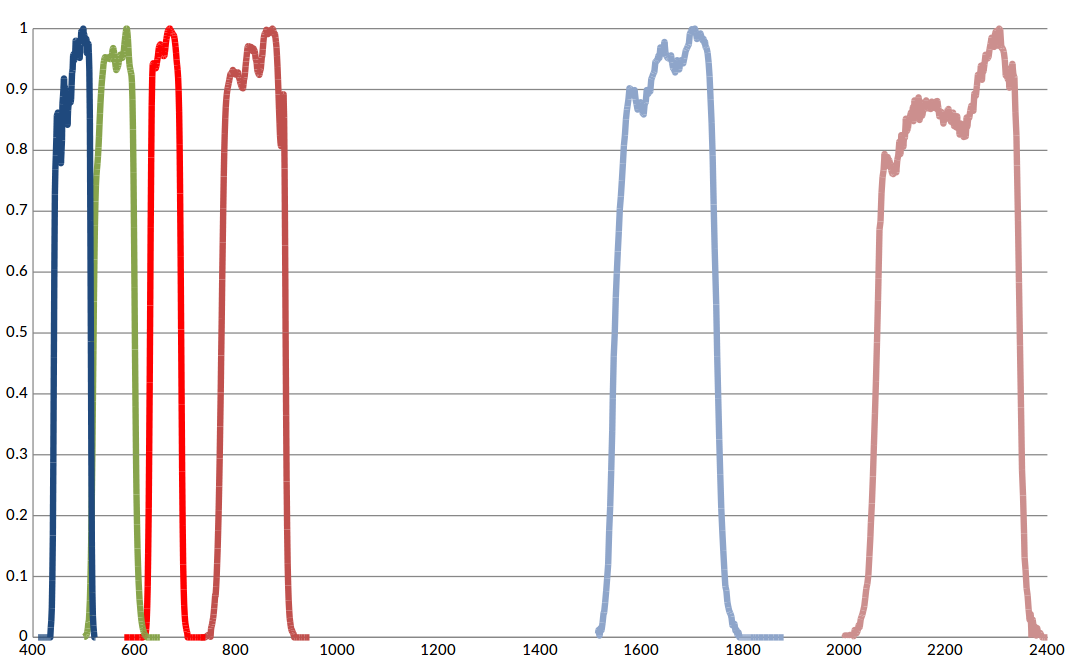
\includegraphics[width=15cm]{./fig/fig_02HSR_Problem/LANDSAT7_MS_RSR}};
            %\node at (nRSR)[xshift=0cm,yshift=6cm] (ntitle) {\Large \textbf{Relative Spectral Response of the Operational TM Sensor in LANDSAT 7 Project}} ;
            \node at (nRSR)[xshift=-8cm,rotate=90] (nylabel) {Spectral Response} ;
            \node at (nRSR)[xshift=0cm,yshift=-5cm] (nxlabel) {Wavelength (nm)} ;
        \end{tikzpicture}
    }
    \caption{Spectral response of the operational TM sensor in
             LANDSAT 7 Project
             \cite{LANDSAT_SPECTRAL_RESPONSE,
                   LANDSAT_HANDBOOK,
                   SPECTRAL_RESPONSE_OF_LANDSAT8}.}
    \label{fig:LANDSAT7_TM_RSR}
\end{figure}
The comparison of spectral characteristics between AVIRIS and TM sensors are
shown in table \ref{table:spectral_characteristics_AVIRIS_TM}.
We can see that a single spectral band of the TM sensor covers multiple
number of AVIRIS spectral bands.
\begin{table}[t]
    \centering
    \begin{tabular}{|c|c|c|l|}
        \hline
        Wavelength ($\mu\,m$) & TM Band & AVIRIS Band & Spectral Band Placement      \\ \hline
        $0.45 - 0.52$         & $1$     & $10 - 16$   & Visible (VIS-B)              \\
        $0.52 - 0.60$         & $2$     & $17 - 24$   & Visible (VIS-G)              \\
        $0.63 - 0.69$         & $3$     & $28 - 35$   & Visible (VIS-R)              \\
        $0.76 - 0.90$         & $4$     & $44 - 57$   & Near Infrared (NIR)          \\
        $1.55 - 1.75$         & $5$     & $127 - 146$ & Short Wave Infrared (SWIR-1) \\
        $10.4 - 12.5$         & $6$     & $-$         & Thermal Infrared (TIR)       \\
        $2.08 - 2.35$         & $7$     & $180 - 208$ & Short Wave Infrared (SWIR-2) \\ \hline
    \end{tabular}
    \caption{Spectral characteristics of TM sensor and AVIRIS sensor
             \cite{AVIRIS,
                   LANDSAT_USING,
                   LANDSAT_HANDBOOK,
                   MILITARY_UTILITY,
                   SPECTRAL_RESPONSE_OF_LANDSAT8}.}
    \label{table:spectral_characteristics_AVIRIS_TM}
\end{table}

\section{Low-Rank Representation of HSIs: the Linear Mixing Model (LMM)}
In the literature, the geoscience and remote sensing community have long
believed HSIs to be high dimensional data with low-rank characteristics
\cite{INTERPRET_RESIDUAL_IMG_SPECTRAL_MIXTURE_ANALYSIS_OF_AVIRIS_IMG,
      BLIND_HU_BY_EXTENDED_LMM,
      CONSTRAINED_SUBPIXEL_TARGET_DETECT_FOR_HSI,
      CONVEX_FORMULATION_HSR_VIA_SUBSPACE_REGULAR,
      DENOIS_HSI_BY_LOWRANK_REPRESENT,
      DISTRIBUT_BLIND_HU_VIA_JOINT_SPARS_LOWRANK_NMF,
      FULLY_CONSTRAINED_LS_LINEAR_SPECTRAL_MIXTURE_ANALYSIS,
      FUMI,
      FUSE,
      HALS_RANK2NMF,
      HSI_RESOTRE_LOWRANK_REPRESENT_SPECTRAL_DIFF_IMG,
      HSI_RESTORE_LOWRANK_MATRIX_RECOVER,
      HSR_BY_JOINTCRITERION_NMF,
      HYSIME,
      JOINT_HSR_AND_HU_INTERACTIVE_FEEDBACK,
      LINEAR_SPECTRAL_RANDOM_MIXTURE_ANALYSIS_FOR_HSI,
      LOWRANK_SUBSPACE_REPRESENT_ESTIMATE_NO_OF_SIGNAL_HSI,
      MVES,
      SNNMF}.
From the low-rank model of HSIs, hyperspectral imagery techniques have been
successfully devised based on the Linear Mixing Model (LMM) \eqref{eq:LMM}
which assumes that the spectral signatures in the HSIs are linearly mixed
\cite{INTERPRET_RESIDUAL_IMG_SPECTRAL_MIXTURE_ANALYSIS_OF_AVIRIS_IMG,
      BLIND_HU_BY_EXTENDED_LMM,
      CNMF,
      CONSTRAINED_SUBPIXEL_TARGET_DETECT_FOR_HSI,
      CONVEX_FORMULATION_HSR_VIA_SUBSPACE_REGULAR,
      DENOIS_HSI_BY_LOWRANK_REPRESENT,
      DISTRIBUT_BLIND_HU_VIA_JOINT_SPARS_LOWRANK_NMF,
      FULLY_CONSTRAINED_LS_LINEAR_SPECTRAL_MIXTURE_ANALYSIS,
      FUMI,
      FUSE,
      HALS_RANK2NMF,
      HSR_BY_JOINTCRITERION_NMF,
      HYSIME,
      ICE,
      JOINT_HSR_AND_HU_INTERACTIVE_FEEDBACK,
      LINEAR_SPECTRAL_RANDOM_MIXTURE_ANALYSIS_FOR_HSI,
      LOWRANK_SUBSPACE_REPRESENT_ESTIMATE_NO_OF_SIGNAL_HSI,
      MVCNMF,
      MVES,
      RVM,
      SISAL,
      SNNMF,
      VCA}.
Specifically, a HSI matrix can be expressed as
\begin{subequations}
    \begin{eqnarray}
        \bm Y & = & \begin{bmatrix} \bm y_1 & \cdots & \bm y_L \end{bmatrix} \\
              & = & \begin{bmatrix} \bm a_1 & \cdots & \bm a_N \end{bmatrix}
                    \begin{bmatrix} \bm s_1 & \cdots & \bm s_L \end{bmatrix} \\
              & = & \begin{bmatrix} \displaystyle \sum_{n=1}^N \bm a_n s_{n,1} & \cdots & \displaystyle \sum_{n=1}^N \bm a_n s_{n,L} \end{bmatrix} \\
              & = & \bm A \bm S,
    \end{eqnarray}
    \label{eq:LMM}
\end{subequations}
where $N$, also called the "model order", is the total number of material in
$\bm Y$; $\bm A \in \R^{M \times N}$ is the endmember matrix that is tall and
contains those $N$ distinct material spectra $\{\bm a_i\}_{i=1}^N$ in the HSI;
$\{\bm s_j\}_{j=1}^L$ is the $N$-dimensional abundance vector at the $j\thtxt$
pixel such that the fat abundance matrix $\bm S \in \R^{N \times L}$ tells the
contribution of the distinct material spectra in the image.
Usually $N$ is assumed to be small, \ie $N \ll \min \{M,L\}$.

Despite the popularity of the LMM model, it is not always true when the acquired HSI
exhibits linearity.
As discussed in
\cite{SPECTRAL_UNMIXING},
LMM is more likely to be valid if the endmembers in a pixel appear in
spatially segregated patterns (Figure \ref{fig:LMM_HOLDS}), while is less
likely to be valid if light is multiply scattered before reaching the sensor
(Figure \ref{fig:LMM_DOESNTHOLD}).
\begin{figure}[t]
    \centering
    \subfigure[$\;$]{\label{fig:LMM_HOLDS}     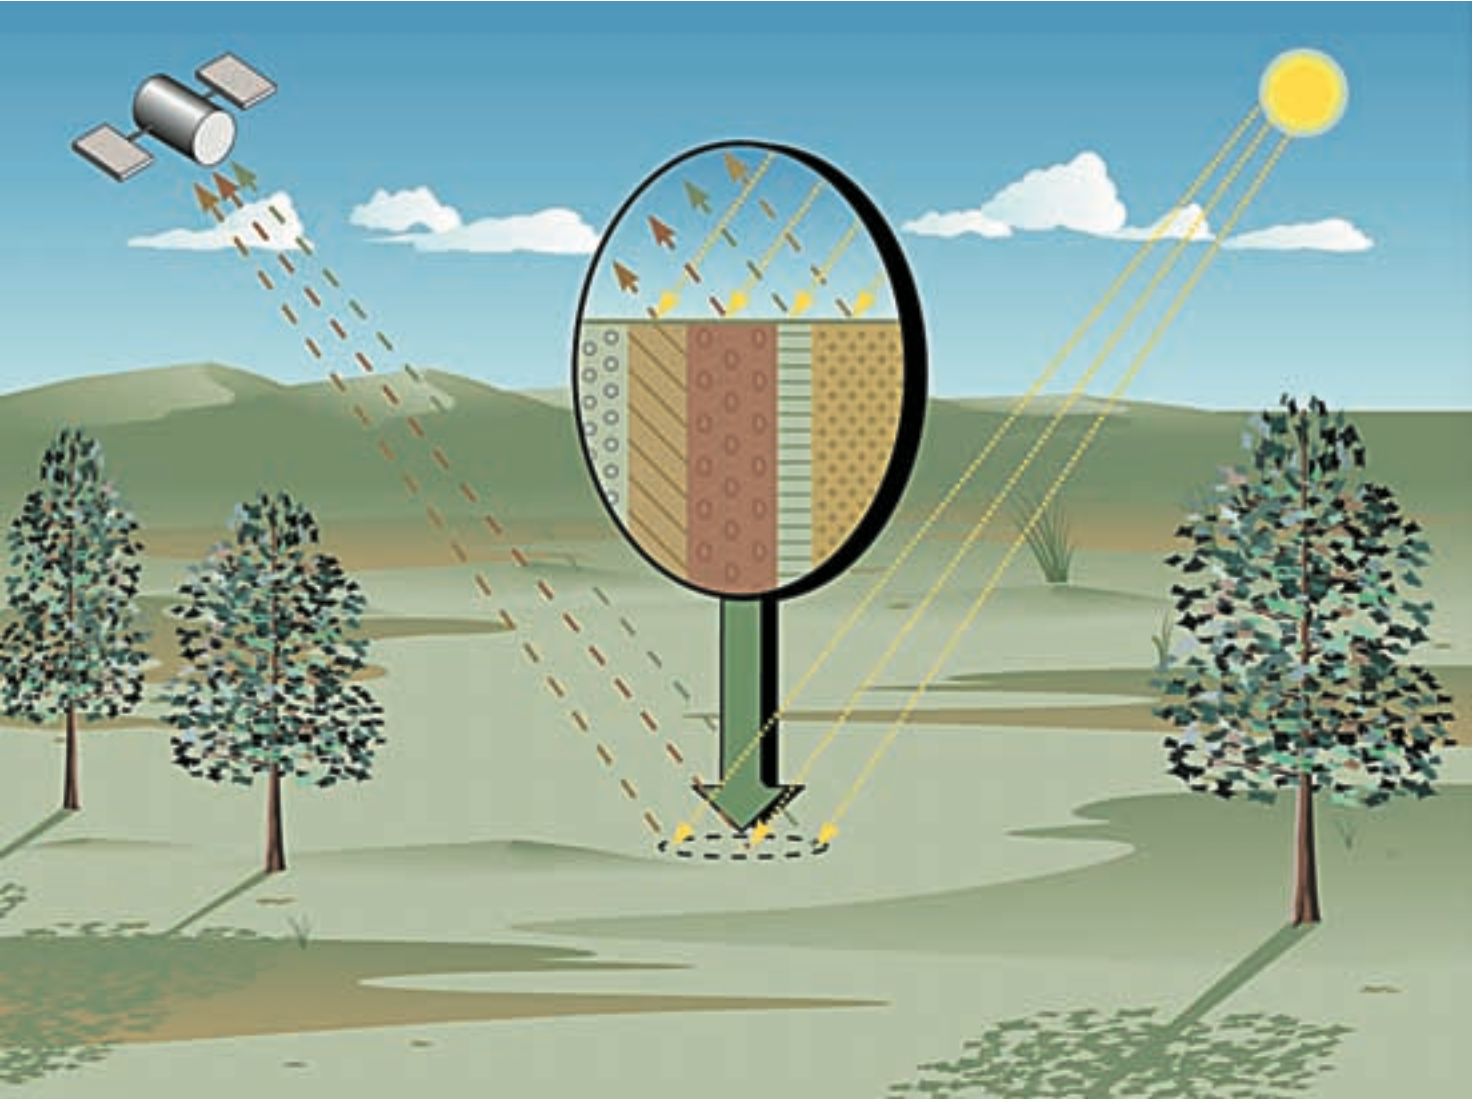
\includegraphics[width=0.48\columnwidth]{./fig/fig_02HSR_Problem/LMM_holds}}
    \subfigure[$\;$]{\label{fig:LMM_DOESNTHOLD}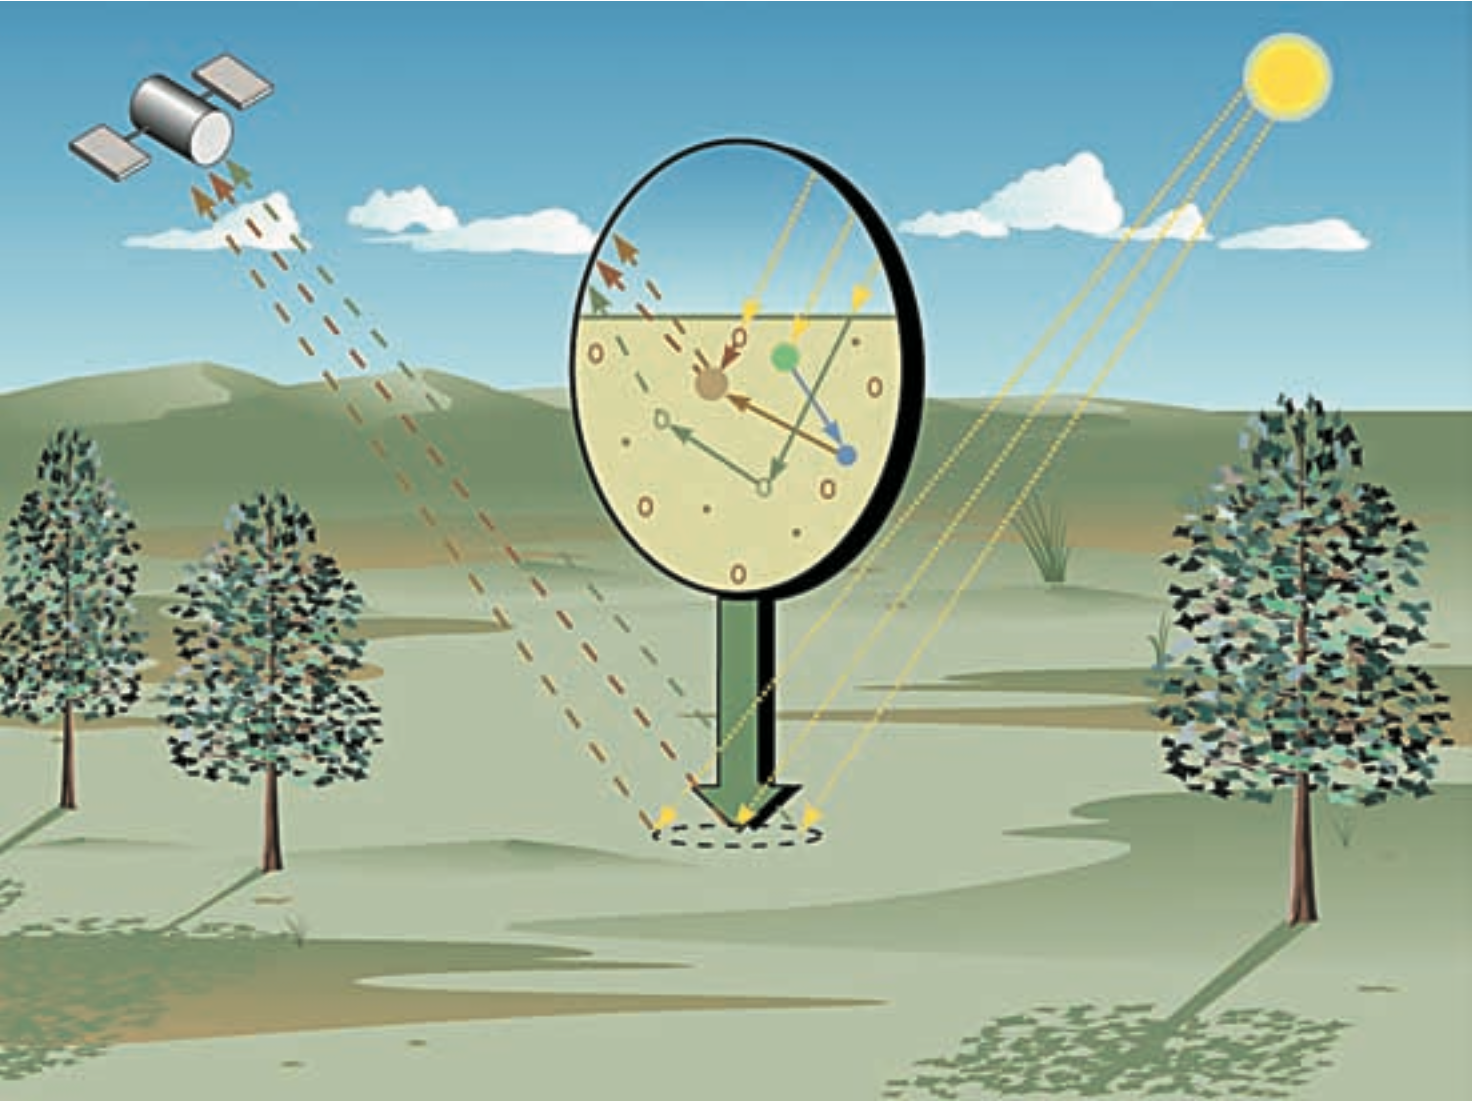
\includegraphics[width=0.48\columnwidth]{./fig/fig_02HSR_Problem/LMM_doesnthold}}
    \caption{Scenarios when LMM is (a) more likely to hold; (b) less likely to hold \cite{SPECTRAL_UNMIXING}.}
\end{figure}
The Earth surface condition in Figure \ref{fig:LMM_HOLDS} can never be met
because Earth surface materials are never naturally arranged in discrete,
segregated patches.
The debate on whether linear or nonlinear mixing processes dominate the real
world scenarios is an unresolved issue.
Nevertheless, LMM is widely regarded as an acceptable model and has been
demonstrated to be valid in a number of laboratory-based studies
\cite{SEMIEMPIRICAL_ANALYSIS_OF_REFLECTANCE_SPECTRA,
      SIMPLE_ALGO_FOR_REMOTE_DETERMINATION_OF_MINERAL_ABUND,
      QUANTITATIVE_ABUND_EST_FROM_BIDIR_REFLECTANCE,
      PHOTO_PHASE_FUNCS_OF_MINERALS}.

\section{The HSR Problem}
By using the spatial and spectral degradation model in
\eqref{eq:spatial_degradation_model_G} and
\eqref{eq:spectral_degradation_model} we may formulate the HSR problem as
\begin{equation}
    \begin{array}{cl}
        \underset{\bm Y}{\min} &
        \displaystyle
        \frac{1}{2} \Vert \YH - \bm Y \bm G \Vert\Fr^2 +
        \frac{1}{2} \Vert \YM - \bm F \bm Y \Vert\Fr^2 \\
        \text{s.t.} &
        \bm Y \in \R_+^{M \times L}.
    \end{array}
    \label{eq:HSR_PROBLEM_WRT_Y}
\end{equation}
Although problem \eqref{eq:HSR_PROBLEM_WRT_Y} is convex, it is an ill-posed
(underdetermined) problem because the objective is to estimate $\bm Y$ from
$\YH$ and $\YM$, that says the problem is to estimate many ($ML$) variables
from few ($ML_\text H + M_\text ML$) observed coefficients (directly from
$\YH$ and $\YM$ to $\bm Y$ in Figure \ref{fig:HSR_problem_visualize}) and thus
the problem has nonunique optimal solutions.
Further, problem \eqref{eq:HSR_PROBLEM_WRT_Y} does not guarantee a low-rank
estimate of HSI.
Therefore, by employing the low-rank LMM model in \eqref{eq:LMM}, problem
\eqref{eq:HSR_PROBLEM_WRT_Y} can be rewritten as
\begin{equation}
    \begin{array}{cl}
        \underset{\bm A,\bm S}{\min} &
        \displaystyle
        \frac{1}{2} \Vert \YH - \bm A \bm S \bm G \Vert\Fr^2 +
        \frac{1}{2} \Vert \YM - \bm F \bm A \bm S \Vert\Fr^2 \\
        \text{s.t.} &
        \begin{array}{cc}
            \bm A \in \mathcal A, &
            \bm S \in \mathcal S,
        \end{array}
    \end{array}
    \label{eq:HSR_PROBLEM_WRT_AS}
\end{equation}
where the Frobenous norm $\Vert \cdot \Vert\Fr^2$ computes the sum-square
error, $\mathcal A \subseteq \R^{M \times N}$ and
$\mathcal S \subseteq \R^{N \times L}$ are the feasible sets of $\bm A$ and
$\bm S$, respectively.
Since the rank of the SR image is bounded by model order $N$, the estimation
problem \eqref{eq:HSR_PROBLEM_WRT_AS} is better than
\eqref{eq:HSR_PROBLEM_WRT_Y} in a sense that the desired SR image
$\hat{\bm Y} = \hat{\bm A} \hat{\bm S}$ has low-rank characteristics.
However, even if $\mathcal A$ and $\mathcal S$ are convex sets, introducing
the low-rank model to the HSR problem sacrifices its convexity so that there
is no guarantee on finding a global optimal solution in problem
\eqref{eq:HSR_PROBLEM_WRT_AS}.
\begin{figure}[t]
    \centering
    \resizebox{0.98\linewidth}{!}{
        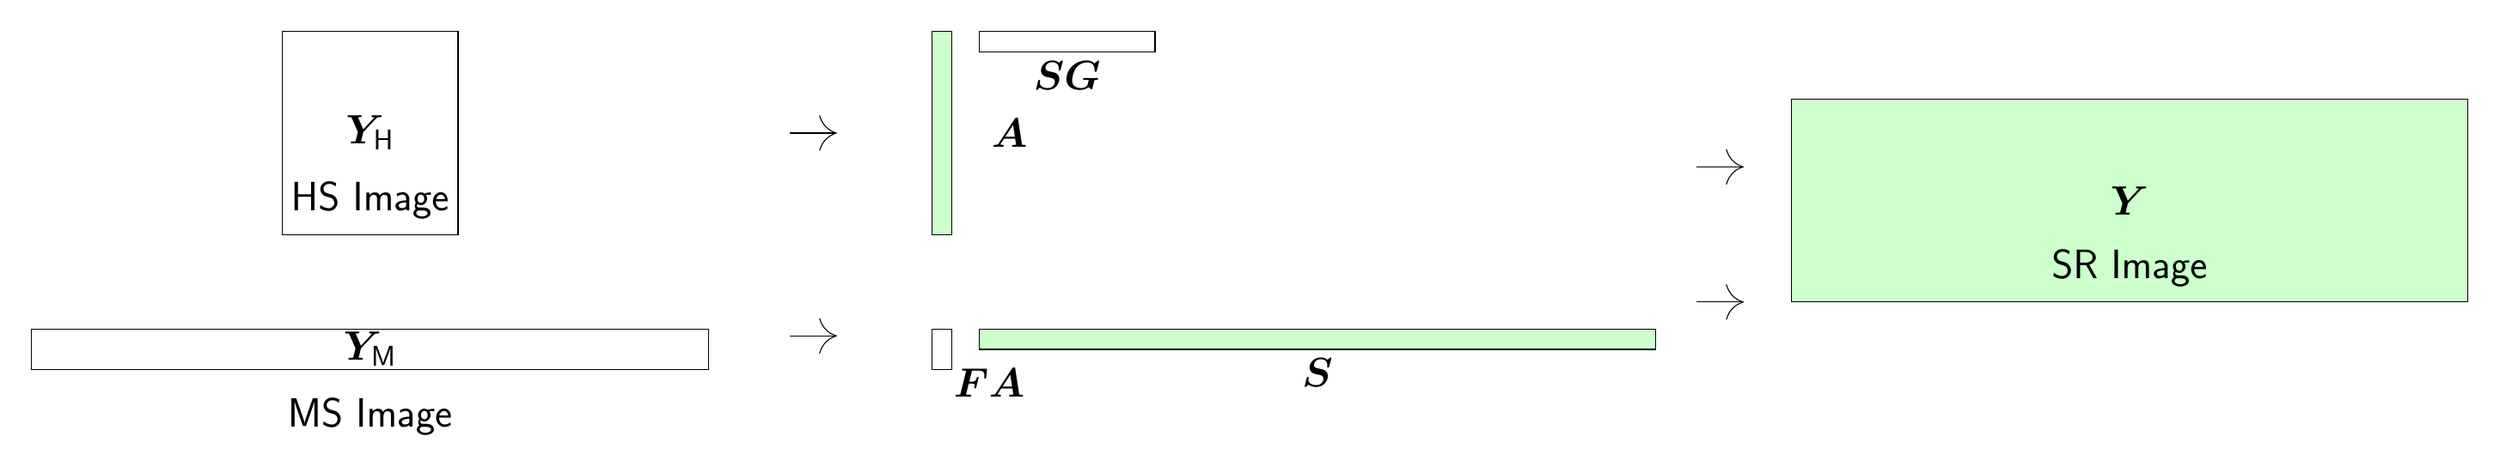
\begin{tikzpicture}
            \node at (-9,0) (nsource) {$\;$} ;
            \node at ( 0,0) (nfactor) {$\;$} ;
            \node at ( 9,0) (nproduc) {$\;$} ;
            % HS Matrix
            \node at (nsource) [xshift=-1.3cm,yshift=5cm] (nYH1) {};
            \node at (nsource) [xshift= 1.3cm,yshift=2cm] (nYH3) {};
            \draw (nYH1) rectangle (nYH3) ;
            \node at ($(nYH1)!0.5!(nYH3)$) (nYH) {\LARGE$\YH$} ;
            \node at ($(nYH1)!0.5!(nYH3)$) [yshift=-1cm] {\LARGE HS Image};
            % MS Matrix
            \node at (nsource) [xshift=  -5cm,yshift=0.6cm] (nYM1) {};
            \node at (nsource) [xshift=   5cm,yshift=0.0cm] (nYM3) {};
            \draw (nYM1) rectangle (nYM3) ;
            \node at ($(nYM1)!0.5!(nYM3)$) (nYH) {\LARGE$\YM$};
            \node at ($(nYM1)!0.5!(nYM3)$) [yshift=-1cm] {\LARGE MS Image};
            % HS factor matrix pair
            \node at (nfactor) [xshift=   0.0cm,yshift=5.0cm] (nSG1) {};
            \node at (nfactor) [xshift=   2.6cm,yshift=4.7cm] (nSG3) {};
            \draw               (nSG1) rectangle (nSG3) ;
            \node at ($(nSG1)!0.5!(nSG3)$) [yshift=-0.5cm] {\LARGE$\bm S \bm G$};
            \node at (nfactor) [xshift=  -0.7cm,yshift=2.0cm] (nA1)  {};
            \node at (nfactor) [xshift=  -0.4cm,yshift=5.0cm] (nA3)  {};
            \draw [fill=green!20] (nA1)  rectangle (nA3)  ;
            \node at ($(nA1)!0.5!(nA3)$) [xshift= 1cm] {\LARGE$\bm A$};
            % MS factor matrix pair
            \node at (nfactor) [xshift=   0.0cm,yshift=0.3cm] (nS1)  {};
            \node at (nfactor) [xshift=  10.0cm,yshift=0.6cm] (nS3)  {};
            \draw [fill=green!20] (nS1)  rectangle (nS3)  ;
            \node at ($(nS1)!0.5!(nS3)$) [yshift=-0.5cm] {\LARGE$\bm S$};
            \node at (nfactor) [xshift=  -0.7cm,yshift=0.0cm] (nFA1) {};
            \node at (nfactor) [xshift=  -0.4cm,yshift=0.6cm] (nFA3) {};
            \draw               (nFA1) rectangle (nFA3) ;
            \node at ($(nFA1)!0.5!(nFA3)$) [xshift=0.7cm,yshift=-0.5cm] {\LARGE$\bm F \bm A$};
            % arrow from HS MS pair to factor pair
            \draw[-{>[scale=2.5,length=3,width=6]}] (-2.8,3.5) -- (-2.1,3.5) ;
            \draw[-{>[scale=2.5,length=3,width=6]}] (-2.8,0.5) -- (-2.1,0.5) ;
            % arrow from factor pair to SR product
            %\draw[-{>[scale=2.5,length=3,width=6]}] (10.6,3.5) -- (11.3,3.0) ;
            %\draw[-{>[scale=2.5,length=3,width=6]}] (10.6,0.5) -- (11.3,1.0) ;
            \draw[-{>[scale=2.5,length=3,width=6]}] (10.6,3.0) -- (11.3,3.0) ;
            \draw[-{>[scale=2.5,length=3,width=6]}] (10.6,1.0) -- (11.3,1.0) ;
            % SR matrix
            \node at (nproduc) [xshift= 3cm,yshift=4cm] (nY1) {};
            \node at (nproduc) [xshift=13cm,yshift=1cm] (nY3) {};
            \draw [fill=green!20] (nY1)  rectangle (nY3)  ;
            \node at ($(nY1)!0.5!(nY3)$) {\LARGE$\bm Y$};
            \node at ($(nY1)!0.5!(nY3)$) [yshift=-1cm]{\LARGE SR Image};
        \end{tikzpicture}
    }
    \caption{Estimate SR image from HS and MS image pair.}
    \label{fig:HSR_problem_visualize}
\end{figure}

\section{The State-of-the-art HSR Formulations and Approaches}

\subsection{HSR Formulation and Approach by Yokoya \etal}
In Yokoya \etal's work, called Coupled Nonnegative Matrix Factorization (CNMF)
\cite{CNMF},
the HSR problem is formulated as
\begin{equation}
    \begin{array}{cl}
        \underset{\bm A ,\bm S}{\min} &
        \displaystyle
        \frac{1}{2} \Vert \YH - \bm A \bm S \bm G \Vert\Fr^2 +
        \frac{1}{2} \Vert \YM - \bm F \bm A \bm S \Vert\Fr^2 \\
        \text{s.t.} &
        \begin{array}{cc}
            \bm A \in \R_+^{M \times N}, &
            \bm S \in \R_+^{N \times L},
        \end{array}
    \end{array}
    \label{eq:HSR_CNMF}
\end{equation}
which has the same formulation as \eqref{eq:HSR_PROBLEM_WRT_AS} by setting
$\mathcal A = \R_+^{M \times N}$ and $\mathcal S = \R_+^{N \times L}$.
In their work problem \eqref{eq:HSR_CNMF} is separated into two independent
subproblems such that they can be individually solved by nonnegative matrix
factorization (NMF) via multiplicative updates (sometimes called Lee-Seung
Algorithm) proposed by Lee and Seung in 1999
\cite{LSMU_NATURE1999,LSMU_NIPS2000},
i.e.
solve the HSR problem by alternatingly solving the two NMF subproblems via
Lee-Seung Algorithm.
In the following part of this section we first review the NMF problem and the
Lee-Seung Algorithm.
Then we present the CNMF algorithm that solves problem \eqref{eq:HSR_CNMF} by
alternating optimization (AO).

\subsubsection{Nonnegative Matrix Factorization (NMF)}
Let $\bm V \in \R_+^{m \times \ell}$ be a rank-$n$ matrix whom we want to
decompose as $\bm V \approx \bm W \bm H$, where $\bm W \in \R_+^{m \times n}$
and $\bm H \in \R_+^{n \times \ell}$.
The NMF problem can be stated as
\begin{equation}
    \begin{array}{cl}
        \underset{\bm W,\bm H}{\min} &
        \Vert \bm V - \bm W \bm H \Vert\Fr^2 \\
        \text{s.t.} &
        \begin{array}{cc}
            \bm W \in \R_+^{m \times n}, &
            \bm H \in \R_+^{n \times \ell}.
        \end{array}
    \end{array}
    \label{eq:NMF}
\end{equation}
Although NMF problem is nonconvex, it is convex with respect to (w.r.t.)
$\bm W$ and $\bm H$ individually.
Usually people attack the NMF problem by AO to find a local optimal solution
by repeating
\begin{eqnarray}
    \bm H\iter{k+1}
    & \gets &
    \arg \; \underset{\bm H \geq \bm 0}{\min}
    \Vert \bm V - \bm W\iter{k} \bm H \Vert\Fr^2, \label{eq:LSMU_updateH}\\
    \bm W\iter{k+1}
    & \gets &
    \arg \; \underset{\bm W \geq \bm 0}{\min}
    \Vert \bm V - \bm W \bm H\iter{k+1} \Vert\Fr^2 \label{eq:LSMU_updateW},
\end{eqnarray}
for some given $\bm W\iter{0}$ and $\bm H\iter{0}$.
The AO algorithm proposed by Lee and Seung is shown in Algorithm
\ref{alg:LSMU}, which is a multiplicative update (MU) type update scheme that
indirectly solves \eqref{eq:LSMU_updateH} and \eqref{eq:LSMU_updateW}.
In the algorithm description, "$*$" and "$/$" represent elementwise
multiplication and division, respectively.
\begin{algorithm}
    \caption{Lee-Seung Algorithm for Nonnegative Matrix Factorization (NMF)}
    \label{alg:LSMU}
	\begin{algorithmic}[1]
        \Require{$\bm V$,
                 $\bm W\iter{0}$,
                 $\bm H\iter{0}$.}
        \smallskip
        \For{$k=0,1,2,\cdots$ until stopping criteria reaches}
            \smallskip
            \Statex{\texttt{// H subproblem}}
            \smallskip
            \State{$\bm H\iter{k,0} \gets \bm H\iter{k}$.}
            \smallskip
            \For{$\ell=1,2,\cdots$}
                \smallskip
                \State{$\bm H\iter{k,\ell} \gets
                        \bm H\iter{k,\ell-1} *
                        ({\bm W\iter{k}}\Tr \bm V) /
                        ({\bm W\iter{k}}\Tr \bm W\iter{k} \bm H\iter{k,\ell-1})$.}
                \smallskip
            \EndFor
            \smallskip
            \State{$\bm H\iter{k+1} \gets \bm H\iter{k,\ell}$.}
            \smallskip
            \Statex{\texttt{// W subproblem}}
            \smallskip
            \State{$\bm W\iter{k,0} \gets \bm W\iter{k}$.}
            \smallskip
            \For{$\ell=1,2,\cdots$}
                \smallskip
                \State{$\bm W\iter{k,\ell} \gets
                        \bm W\iter{k,\ell-1} *
                        (\bm V {\bm H\iter{k+1}}\Tr) /
                        (\bm W\iter{k,\ell-1} \bm H\iter{k+1} {\bm H\iter{k+1}}\Tr)$.}
                \smallskip
            \EndFor
            \smallskip
            \State{$\bm W\iter{k+1} \gets \bm W\iter{k,\ell}$.}
            \smallskip
        \EndFor
        \smallskip
        \Ensure{$\bm W\iter{k+1}$,$\bm H\iter{k+1}$.}
    \end{algorithmic}
\end{algorithm}

\subsubsection{Coupled Nonnegative Matrix Factorization (CNMF)}
Let
\[ \hat{\bm W},\,\hat{\bm H}\,\gets\,\texttt{LeeSeung}(\bm V,\bm W',\bm H')\]
denote the process of solving the NMF problem \eqref{eq:NMF} by Algorithm
\ref{alg:LSMU} using $\bm W'$ and $\bm H'$ as the algorithm input.
Yokoya \etal tackle the HSR problem by applying the Lee-Seung Algorithm to
alternatingly factorize $\YH$ and $\YM$ to obtain the desired endmember and
abundance matrix pair.
Rather than directly solve problem \eqref{eq:HSR_CNMF}, CNMF starts from
initial guess on matrix $\bm A\iter{0}$ and $\bm S\iter{0}$.
Then, with $\bm E\iter{0} = \bm F \bm A\iter{0}$ and
$\bm R\iter{0} = \bm S\iter{0} \bm G$, CNMF solves the HSR problem by repeating
\eqref{eq:CNMF_update_A_subproblem} and \eqref{eq:CNMF_update_S_subproblem}
below:

\begin{subequations}
\begin{eqnarray}
    % =======================
    % 1st part of CNMF update
    % =======================
    %\begin{array}{c} \bm A\iter{k+1}\;,\;\bm R' \\ \; \end{array}
    %&
    %\begin{array}{c} \gets \\ \; \end{array}
    %&
    %\begin{array}{ccl}\arg & \underset{\bm A, \bm R}{\min} & \Vert \YH - \bm A \bm R \Vert\Fr^2 \\
    %                       & \text{s.t.}                   & \bm A \geq 0 \;,\; \bm R \geq 0, \end{array} \\
    \bm A\iter{k+1}, \bm R' & \gets & \texttt{LeeSeung}(\YH,\bm A\iter{k},\bm R\iter{k}) \\
    % =======================
    % 2nd part of CNMF update
    % =======================
    \bm E\iter{k+1} & \gets & \bm F \bm A\iter{k+1},
    %\bm A & \gets & \bm A\iter{k+1},
\end{eqnarray}
\label{eq:CNMF_update_A_subproblem}
\end{subequations}
\begin{subequations}
\begin{eqnarray}
    % =======================
    % 3rd part of CNMF update
    % =======================
    %\begin{array}{c} \bm E'\;,\;\bm S\iter{k+1} \\ \; \end{array}
    %&
    %\begin{array}{c} \gets \\ \; \end{array}
    %&
    %\begin{array}{ccl}\arg & \underset{\bm E, \bm S}{\min} & \Vert \YM - \bm E \bm S \Vert\Fr^2 \\
    %                       & \text{s.t.}                   & \bm E \geq 0 \;,\; \bm S \geq 0, \end{array} \\
    \bm E', \bm S\iter{k+1} & \gets & \texttt{LeeSeung}(\YM,\bm E\iter{k+1},\bm S\iter{k}) \\
    % =======================
    % 4th part of CNMF update
    % =======================
    \bm R\iter{k+1} & \gets & \bm S\iter{k+1} \bm G.
    %\bm S & \gets & \bm S\iter{k+1},
\end{eqnarray}
\label{eq:CNMF_update_S_subproblem}
\end{subequations}
$\bm A\iter{K+1}$ and $\bm S\iter{K+1}$ are the desired endmember and
abundance matrix pair, respectively; $\bm E\iter{K+1}$ and $\bm R\iter{K+1}$
are the byproduct matrix pair.
The CNMF algorithm is shown in Algorithm \ref{alg:HSR_CNMF}.
The recovered SR image by CNMF can be obtained by
$\hat{\bm Y} = \bm A\iter{k+1}\bm S\iter{k+1}$.

Despite its efficiency and ease of implementation, we remark that the
algorithm is an indirect approach to solve \eqref{eq:HSR_CNMF} because MS
recovery error does not take part in the endmember estimation, and the same
goes for the HS recovery error in abundance estimation.
An online available program code of CNMF can be found from Yokoya's homepage
\footnotemark.
\footnotetext[1]{Matlab implementation can be found in
http://naotoyokoya.com/Download.html.
Note that in their implementation they attempt to enforce some further
constraints on the variables by using tricks suggested in
\cite{FULLY_CONSTRAINED_LS_LINEAR_SPECTRAL_MIXTURE_ANALYSIS}.
However in this thesis we reimplement CNMF to exactly follow the algorithm
description in Yokoya's paper.}
\begin{algorithm}[H]
    \caption{Coupled Nonnegative Matrix Factorization (CNMF)}
    \label{alg:HSR_CNMF}
	\begin{algorithmic}[1]
        \Require{$\YH$,
                 $\YM$,
                 $\bm F$,
                 $\bm G$,
                 $\bm A\iter{0}$,
                 $\bm S\iter{0}$.}
        \For{$k=0,1,2,\cdots$ until stopping criteria reaches}
            \Statex{\texttt{// Hyperspectral Subproblem}}
            \State{$\bm R\iter{k} \gets \bm S\iter{k} \bm G$, $\bm R\iter{k,0} \gets \bm R\iter{k}$, $\bm A\iter{k,0} \gets \bm A\iter{k}$.}
            \For{$\ell=1,2,\cdots$}
                \State{$\bm R\iter{k,\ell} \gets
                        \bm R\iter{k,\ell-1} *
                        ({\bm A\iter{k,\ell-1}}\Tr \YH) /
                        ({\bm A\iter{k,\ell-1}}\Tr \bm A\iter{k,\ell-1} \bm R\iter{k,\ell-1})$.}
                \State{$\bm A\iter{k,\ell} \gets
                        \bm A\iter{k,\ell-1} *
                        (\YH {\bm R\iter{k,\ell}}\Tr) /
                        (\bm A\iter{k,\ell-1} \bm R\iter{k,\ell} {\bm R\iter{k,\ell}}\Tr)$.}
            \EndFor
            \State{$\bm A\iter{k+1} \gets \bm A\iter{k,\ell}$.}
            \Statex{\texttt{// Multispectral Subproblem}}
            \State{$\bm E\iter{k} \gets \bm F \bm A\iter{k+1}$, $\bm S\iter{k,0} \gets \bm S\iter{k}$, $\bm E\iter{k,0} \gets \bm E\iter{k}$.}
            \For{$\ell=1,2,\cdots$}
                \State{$\bm S\iter{k,\ell} \gets
                        \bm S\iter{k,\ell-1} *
                        ({\bm E\iter{k,\ell-1}}\Tr \YM) /
                        ({\bm E\iter{k,\ell-1}}\Tr \bm E\iter{k,\ell-1} \bm S\iter{k,\ell-1})$.}
                \State{$\bm E\iter{k,\ell} \gets
                        \bm E\iter{k,\ell-1} *
                        (\YM {\bm S\iter{k,\ell}}\Tr) /
                        (\bm E\iter{k,\ell-1} \bm S\iter{k,\ell} {\bm S\iter{k,\ell}}\Tr)$.}
            \EndFor
            \State{$\bm S\iter{k+1} \gets \bm S\iter{k,\ell}$.}
        \EndFor
        \Ensure{$\bm A\iter{k+1},\bm S\iter{k+1}$.}
    \end{algorithmic}
\end{algorithm}

\subsection{HSR Formulation and Approach by Wei \etal}
In Wei \etal's work, called "Fusion based on Unmixing for Multiband Images
(FUMI)"
\cite{FUMI},
the HSR problem is formulated as
\begin{equation}
    \begin{array}{cl}
        \underset{\bm A ,\bm S}{\min} &
        \displaystyle
        \frac{1}{2} \Vert \YH - \bm A \bm S \bm G \Vert\Fr^2 +
        \frac{1}{2} \Vert \YM - \bm F \bm A \bm S \Vert\Fr^2 \\
        \text{s.t.} &
        \begin{array}{ccc}
            \bm A \in [0,1]^{M \times N}, &
            \bm S \in \triangle^{N \times L},
            %\bm S \in \R_+^{N \times L}, &
            %\bm s_j \in \mathcal{U}_N, \text{ for } j = 1,\cdots,L,
        \end{array}
    \end{array}
    \label{eq:HSR_FUMI}
\end{equation}
where
\begin{equation}
    \triangle^{N \times L} = \{\bm X \in \R_+^{N \times L} \; \big| \;
                               \bm 1_N\Tr \bm x_i = 1      \; ,     \;
                               \forall \; i\}
    \label{eq:simplex}
\end{equation}
denotes a set of matrix that is nonnegative and columnwise sum-to-one.
Similar to CNMF, Wei \etal apply AO to the HSR problem by splitting it into
two.
Their formulation differs from CNMF by having more constraints on the decision
variables, \ie in addition to nonnegative constraints on the variables, the
endmember matrix is further bounded from above by $\bm 1$ and the abundance
matrix is forced to be on a unit simplex.
Their approach to solving the HSR problem is also different from CNMF such
that both HS and MS recovery error are considered in both subproblems.
Due to the extra constraints, they solve the subproblems by Alternating
Direction Method of Multipliers (ADMM)
\cite{ADMM_BOYD2011},
an algorithm that efficiently handles convex constrained quadratic program (QP).
In the following part of this section, we first review the ADMM algorithm and
solving QP by ADMM.
Then the algorithm details of FUMI are presented.

\subsubsection{Alternating Direction Method of Multipliers (ADMM)}
ADMM, popularized by Boyd \etal in 2010
\cite{ADMM_BOYD2011},
is an algorithm that solves problems with the following structure:
\begin{equation}
    \begin{array}{cl}
        \underset{\bm x \in \R^n, \bm z \in \R^m}{\min} &
        f(\bm x) + g(\bm z) \\
        \text{s.t.} &
        \bm P \bm x + \bm Q \bm z = \bm r,
    \end{array}
    \label{eq:ADMM}
\end{equation}
where $\bm P\in\R^{k \times n}$, $\bm Q\in\R^{k \times m}$ and $\bm r\in\R^k$;
$f$ and $g$ are convex functions.
By defining the Augmented Lagrangian of problem \eqref{eq:ADMM} as
\begin{equation}
    L_\mu(\bm x,\bm z,\bm y) = 
    f(\bm x) + g(\bm z) + \bm y\Tr(\bm P \bm x + \bm Q \bm z - \bm r) +
    \frac{\mu}{2} \Vert \bm P \bm x + \bm Q \bm z - \bm r \Vert_2^2,
\end{equation}
where $\bm y \in \R^p$ is called the dual variable; $\mu > 0$ is a positive
constant, the ADMM algorithm that solves problem \eqref{eq:ADMM} is presented
in Algorithm \ref{alg:ADMM}. Its general convergence analysis can be found in
\cite{ADMM_BOYD2011,
      ADMM_GENERAL_CONVERG_ANALYSIS,
      LINEAR_CONVERG_OF_ADMM}.
\begin{algorithm}[H]
    \caption{Alternating Direction Method of Multipliers (ADMM)}
    \label{alg:ADMM}
	\begin{algorithmic}[1]
        \Require{$\bm x\iter{0}$,
                 $\bm z\iter{0}$,
                 $\bm y\iter{0}$.}
        \For{$i=1,2,\cdots$ until stopping criteria reaches}
            \State{$\bm x\iter{i} \gets
                    \arg \; \underset{\bm x}{\min} \;
                    L_\mu(\bm x,\bm z\iter{i-1},\bm y\iter{i-1})$.}
            \State{$\bm z\iter{i} \gets
                    \arg \; \underset{\bm z}{\min} \;
                    L_\mu(\bm x\iter{i},\bm z,\bm y\iter{i-1})$.}
            \State{$\bm y\iter{i} \gets \bm y\iter{i-1} +
                    \mu (\bm P \bm x\iter{i} + \bm Q \bm z\iter{i} - \bm r)$.}
        \EndFor
        \Ensure{$\bm x\iter{i},\bm z\iter{i}$.}
    \end{algorithmic}
\end{algorithm}
%Problem \eqref{eq:ADMM} has a special case such that the problem is a QP
QP is a special case of problem \eqref{eq:ADMM}.
A standard QP can be written as follows:
\begin{equation}
    \begin{array}{cl}
        \underset{\bm x}{\min} &
        \displaystyle \frac{1}{2} \bm x\Tr \bm B \bm x + \bm c\Tr \bm x \\
        \text{s.t.} & \bm x \in \mathcal X,
    \end{array}
\end{equation}
where $\mathcal X \subseteq \R^n$ is a convex feasible set of $\bm x$.
If we let
\begin{eqnarray}
    \bm P    & = & \bm I, \nonumber \\
    \bm Q    & = & -\bm I, \nonumber \\
    \bm r    & = & \bm 0, \nonumber \\
    f(\bm x) & = & \frac{1}{2} \bm x\Tr \bm B \bm x + \bm c\Tr \bm x, \nonumber \\
    g(\bm z) & = & \mathcal I_{\mathcal X}(\bm z) \nonumber \\
             & = & \begin{cases}
                       0,       & \bm z \in    \mathcal X \\
                       +\infty, & \bm z \notin \mathcal X,
                   \end{cases}, \nonumber
\end{eqnarray}
where $\mathcal I_{\mathcal X}(\cdot)$ is an indicator function w.r.t. convex set
$\mathcal X$, then problem \eqref{eq:ADMM} becomes a convex constrained QP.

\subsubsection{Fusion based on Unmixing for Multiband Images (FUMI)}
The problem formulation by Wei \etal is splitted into $\bm S$ subproblem and
$\bm A$ subproblem.
The subproblems are listed below.
\begin{align}
    &
    \begin{array}{cl}
        \underset{\bm S}{\min} &
        \displaystyle
        \frac{1}{2} \Vert \YH - \bm A \bm S \bm G \Vert\Fr^2 +
        \frac{1}{2} \Vert \YM - \bm F \bm A \bm S \Vert\Fr^2 \\
        \text{s.t.} &
        \bm S \in \triangle^{N \times L},
    \end{array}
    \label{eq:HSR_FUMI_S-subproblem}
    \\
    &
    \begin{array}{cl}
        \underset{\bm A}{\min} &
        \displaystyle
        \frac{1}{2} \Vert \YH - \bm A \bm S \bm G \Vert\Fr^2 +
        \frac{1}{2} \Vert \YM - \bm F \bm A \bm S \Vert\Fr^2 \\
        \text{s.t.} &
        \bm A \in [0,1]^{M \times N}.
    \end{array}
    \label{eq:HSR_FUMI_A-subproblem}
\end{align}
And the Augmented Lagrangian of $\bm S$ and $\bm A$ subproblems of
\eqref{eq:HSR_FUMI_S-subproblem} become
\begin{eqnarray}
    \mathcal L_S(\bm A, \bm S, \bm \Sigma, \bm \varPsi)
    & = &
    \displaystyle
    \frac{1}{2} \Vert \YH - \bm A \bm S \bm G \Vert\Fr^2 +
    \frac{1}{2} \Vert \YM - \bm F \bm A \bm S \Vert\Fr^2 \nonumber \\
    &   &
    + \mathcal I_{\triangle^{N \times L}}(\bm \Sigma) +
    \langle \bm S - \bm \Sigma , \bm \varPsi \rangle +
    \displaystyle \frac{\mu}{2} \Vert \bm S - \bm \Sigma \Vert\Fr^2
    \label{eq:HSR_FUMI_Lagragian_S-subproblem}
\end{eqnarray}
and
\begin{eqnarray}
    \mathcal L_A(\bm A, \bm S, \bm \Lambda, \bm \varPhi)
    & = &
    \displaystyle
    \frac{1}{2} \Vert \YH - \bm A \bm S \bm G \Vert\Fr^2 +
    \frac{1}{2} \Vert \YM - \bm F \bm A \bm S \Vert\Fr^2 \nonumber \\
    &   &
    + \mathcal I_{[0,1]^{M \times N}}(\bm \Lambda) +
    \langle \bm A - \bm \Lambda , \bm \varPhi \rangle +
    \displaystyle \frac{\mu}{2} \Vert \bm A - \bm \Lambda \Vert\Fr^2,
    \label{eq:HSR_FUMI_Lagrangian_A_subproblem}
\end{eqnarray}
where $\bm \Sigma$ and $\bm \Lambda$ are the split variables; $\bm \varPsi$
and $\bm \varPhi$ are the dual variable of $\bm S$ and $\bm A$ subproblems,
respectively, and $\mu > 0$.
FUMI is therefore presented as in Algorithm \ref{alg:HSR_FUMI}
\footnotemark.
\footnotetext[2]{The Matlab implementation of FUMI can be found in
author's GitHub page https://github.com/qw245/FUMI.
Note that in their implementation the algorithm does not solve the subproblems
properly because the convergence of ADMM is not checked.
Besides they perform subspace projection before solving the subproblems in
order to reduce computation cost.
In this thesis, however, we modify FUMI to exactly follow the algorithm
description in Wei's paper.}
\begin{algorithm}[H]
    \caption{Fusion based on Unmixing for Multiband Images (FUMI)}
    \label{alg:HSR_FUMI}
    \begin{algorithmic}[1]
        \Require{$\YH$,
                 $\YM$,
                 $\bm F$,
                 $\bm G$,
                 $\bm A\iter{0}$,
                 $\bm S\iter{0}$}
        \State{$\bm \Sigma\iter{0}  \gets \bm S\iter{0}$,
               $\bm \varPsi\iter{0} \gets \bm 0$,
               $\bm \Lambda\iter{0} \gets \bm A\iter{0}$,
               $\bm \varPhi\iter{0} \gets \bm0$.}
        \For{$k=1,2,\cdots$ until stopping criteria reaches}
            \Statex{\texttt{// S-Subproblem}}
            \State{$\bm S      \iter{k,0} \gets \bm S      \iter{k}$,
                   $\bm \Sigma \iter{k,0} \gets \bm \Sigma \iter{k}$,
                   $\bm \varPsi\iter{k,0} \gets \bm \varPsi\iter{k}$.}
            \For{$\ell=1,2,\cdots$}
            \State{$\bm S\iter{k,\ell} \gets
                    \arg\;\underset{\bm S}{\min} \;
                    \mathcal L_S\left(\bm A\iter{k}             ,
                                      \bm S                     ,
                                      \bm \Sigma \iter{k,\ell-1},
                                      \bm \varPsi\iter{k,\ell-1}\right)$.}
            \State{$\bm \Sigma\iter{k,\ell} \gets
                    \arg\;\underset{\bm \Sigma}{\min} \;
                    \mathcal L_S\left(\bm A\iter{k}             ,
                                      \bm S\iter{k,\ell}        ,
                                      \bm \Sigma                ,
                                      \bm \varPsi\iter{k,\ell-1}\right)$.}
            \State{$\bm \varPsi\iter{k,\ell} \gets \bm \varPsi\iter{k,\ell-1}
                    - \left(\bm S\iter{k,\ell} - \bm \Sigma\iter{k,\ell}\right)$.}
            \EndFor
            \State{$\bm S      \iter{k+1} \gets \bm S      \iter{k,\ell}$,
                   $\bm \Sigma \iter{k+1} \gets \bm \Sigma \iter{k,\ell}$,
                   $\bm \varPsi\iter{k+1} \gets \bm \varPsi\iter{k,\ell}$.}
            \Statex{\texttt{// A-Subproblem}}
            \State{$\bm A      \iter{k,0} \gets \bm S       \iter{k}$,
                   $\bm \Lambda\iter{k,0} \gets \bm \Lambda \iter{k}$,
                   $\bm \varPhi\iter{k,0} \gets \bm \varPhi\iter{k}$.}
            \For{$\ell=1,2,\cdots,L$}
            \State{$\bm A\iter{k,\ell} \gets
                    \arg\;\underset{\bm A}{\min} \;
                    \mathcal L_A\left(\bm A                     ,
                                      \bm S\iter{k+1}           ,
                                      \bm \Lambda\iter{k,\ell-1},
                                      \bm \varPhi\iter{k,\ell-1}\right)$.}
            \State{$\bm \Lambda\iter{k,\ell} \gets
                    \arg\;\underset{\bm \Lambda}{\min} \;
                    \mathcal L_A\left(\bm A\iter{k,\ell}        ,
                                      \bm S\iter{k+1}           ,
                                      \bm \Lambda               ,
                                      \bm \varPhi\iter{k,\ell-1}\right)$.}
            \State{$\bm \varPhi\iter{k,\ell} \gets \bm \varPhi\iter{k,\ell-1}
                    - \left(\bm A\iter{k,\ell} - \bm \Lambda\iter{k,\ell}\right)$.}
            \EndFor
            \State{$\bm A      \iter{k+1} \gets \bm A      \iter{k,\ell}$,
                   $\bm \Lambda\iter{k+1} \gets \bm \Lambda\iter{k,\ell}$,
                   $\bm \varPhi\iter{k+1} \gets \bm \varPhi\iter{k,\ell}$.}
        \EndFor
        \Ensure{$\bm A\iter{k+1}$, $\bm S\iter{k+1}$}
    \end{algorithmic}
\end{algorithm}
Similar to CNMF, FUMI recovers the estimated SR image by
$\hat{\bm Y} = \bm A\iter{k+1}\bm S\iter{k+1}$.

\subsection{General Review on the State of the Arts}
The discussed state-of-the-art HSR problem formulations can be decomposed to
convex subproblems.
To solve them the CNMF and FUMI algorithms use the famous Lee-Seung Algorithm
and ADMM, respectively.
CNMF uses Lee-Seung Algorithm because this algorithm handles NMF-type problems
efficiently.
On the contrary, however, CNMF is a less flexible algorithm because the factor
matrix pair constraints are limited to be nonnegative orthant and cannot be
easily extended to other constraints.
%Slightly changing the constraints could make the CNMF algorithm less suitable
%although Yokoya \etal suggests a possible modification of CNMF algorithm by
%employing a trick mentioned in
%\cite{FULLY_CONSTRAINED_LS_LINEAR_SPECTRAL_MIXTURE_ANALYSIS}.
FUMI uses ADMM to solve the convex subproblems.
A possible drawback is that ADMM may cost too much runtime if the spectral
images size grows to very large scale.
 % HSR Problems and Related Works
\chapter{HSR with First-Order Gradient Methods (FOGMs)}

In this chapter we discuss an inexact BCD approach to tackle the HSR problem,
namely ALternating Gradient-based Optimization (ALGO) using FOGMs.
The organization of this chapter is as follows.
We first express the subproblems of the HSR problem as convex constrained QP.
Then we give a review on a few kind of FOGMs that solve this QP.
After that a traditional algorithm framework that solves the HSR problem by
exact BCD is presented, followed by our proposed algorithm framework ALGO.
We also show the specific algorithm implementation of ALGO using each of the
discussed FOGM at the end of this chapter.

\section{HSR Problem as Convex Constrained QPs}
The general HSR problem is re-stated below.
\begin{equation}
    \begin{array}{cl}
        \underset{\bm A,\bm S}{\min} &
        \displaystyle
        \frac{1}{2} \Vert \YH - \bm A \bm S \bm G \Vert\Fr^2 +
        \frac{1}{2} \Vert \YM - \bm F \bm A \bm S \Vert\Fr^2 \\
        \text{s.t.} &
        \begin{array}{cc}
            \bm A \in \mathcal A, & \bm S \in \mathcal S.
        \end{array}
    \end{array} \tag{$*$}
    \label{eq:HSR_problem_CH3}
\end{equation}
Problem \eqref{eq:HSR_problem_CH3} is separately convex in $\bm S$ and in
$\bm A$.
The $\bm S$ and $\bm A$ subproblem of \eqref{eq:HSR_problem_CH3} can be
expressed as
\begin{align}
    &
    \begin{array}{cl}
        \underset{\bm S}{\min} &
        \displaystyle
        \frac{1}{2} \Vert \YH - \bm A \bm S \bm G \Vert\Fr^2 +
        \frac{1}{2} \Vert \YM - \bm F \bm A \bm S \Vert\Fr^2 \\
        \text{s.t.} &
        \bm S \in \mathcal S,
    \end{array} \tag{$\eqmathcal S$}
    \label{eq:HSR_S-subproblem_CH3} \\
    &
    \begin{array}{cl}
        \underset{\bm A}{\min} &
        \displaystyle
        \frac{1}{2} \Vert \YH - \bm A \bm S \bm G \Vert\Fr^2 +
        \frac{1}{2} \Vert \YM - \bm F \bm A \bm S \Vert\Fr^2 \\
        \text{s.t.} &
        \bm A \in \mathcal A,
    \end{array} \tag{$\eqmathcal A$}
    \label{eq:HSR_A-subproblem_CH3}
\end{align}
respectively.
We see that the objective function of \eqref{eq:HSR_S-subproblem_CH3} and
\eqref{eq:HSR_A-subproblem_CH3} can be expressed in least squares form using
the Kronecker product equality
\begin{equation}
    \vectxt{\bm P \bm X \bm Q} =
    \begin{bmatrix} \bm Q\Tr \otimes \bm P \end{bmatrix} \vectxt{\bm X},
\end{equation}
where $\bm P \in \R^{m \times n}$; $\bm X \in \R^{n \times p}$;
$\bm Q \in \R^{p \times q}$; $\otimes$ denotes the Kronecker product and
$\vectxt{\cdot}$ is an operation that lexicographically concatenate all
columns of the argument matrix to form a single column.
\ie $\bm x = \vectxt{\bm X} \in \R^{np}$.
Let $\bm s=\vectxt{\bm S}$, $\bm a=\vectxt{\bm A}$, $\yH=\vectxt{\YH}$,
$\yM=\vectxt{\YM}$.
Then \eqref{eq:HSR_S-subproblem_CH3} and \eqref{eq:HSR_A-subproblem_CH3}
are equivalent to
\begin{equation}
    \begin{array}{cl}
        \underset{\bm s}{\min} &
        \displaystyle
        \frac{1}{2} \Vert \bm y - \bm H_S \bm s \Vert_2^2
        \\%= \frac{1}{2} \bm s\Tr \bm H_S\Tr \bm H_S \bm s -
          %\bm y\Tr \bm H_S \bm s + \frac{1}{2} \bm y\Tr \bm y \\
        \text{s.t.} &
        \begin{array}{cc}
            \bm S \in \mathcal S, & \bm s = \vectxt{\bm S}
        \end{array}
    \end{array} \tag{$\eqmathcal s$}
    \label{eq:HSR_s-subproblem}
\end{equation}
and
\begin{equation}
    \begin{array}{cl}
        \underset{\bm a}{\min} &
        \displaystyle
        \frac{1}{2} \Vert \bm y - \bm H_A \bm a \Vert_2^2
        \\%= \frac{1}{2} \bm a\Tr \bm H_A\Tr \bm H_A \bm a -
          %\bm y\Tr \bm H_A \bm a + \frac{1}{2} \bm y\Tr \bm y \\
        \text{s.t.} &
        \begin{array}{cc}
            \bm A \in \mathcal A, & \bm a = \vectxt{\bm A},
        \end{array} \tag{$\eqmathcal a$}
    \end{array}
    \label{eq:HSR_a-subproblem}
\end{equation}
respectively, in which
\[ \bm y   = \begin{bmatrix} \yH \\ \yM \end{bmatrix}; \;\;\;
   \bm H_S = \begin{bmatrix} \bm G\Tr \otimes \bm A \\
                             \bm I_L  \otimes \bm{FA} \end{bmatrix}; \;\;\;
   \bm H_A = \begin{bmatrix} (\bm{SG})\Tr \otimes \bm I_M \\
                                 \bm S\Tr    \otimes \bm A \end{bmatrix}.\]
In the remaining chapters, we focus our discussion of FOGMs on the QPs
\eqref{eq:HSR_s-subproblem} and \eqref{eq:HSR_a-subproblem}.
To see they are QPs we let $f_s(\bm s)$ and $f_a(\bm a)$ be their
objective functions and observe that
\begin{equation}
    f_s(\bm s)
    =
    \displaystyle \frac{1}{2} \bm s\Tr \bm H_S\Tr \bm H_S \bm s -
    \bm y\Tr \bm H_S \bm s + \frac{1}{2} \bm y\Tr \bm y
    \label{eq:HSR_s-subproblem_expandedform}
\end{equation}
and
\begin{equation}
    f_a(\bm a)
    =
    \displaystyle \frac{1}{2} \bm a\Tr \bm H_A\Tr \bm H_A \bm a -
    \bm y\Tr \bm H_A \bm a + \frac{1}{2} \bm y\Tr \bm y
    \label{eq:HSR_a-subproblem_expandedform}
\end{equation}
both attain a quadratic form.
Also, either using Yokoya \etal's formulation or Wei \etal's formulation, the
constraints of \eqref{eq:HSR_s-subproblem} and \eqref{eq:HSR_a-subproblem} are
all convex.
%To see this, let us consider the constrains in the two formulations one by one.
Specifically, we may consider:
\begin{itemize}
    \item Yokoya \etal's formulation: \newline
          $\mathcal S=\R_+^{N \times L}$ and $\mathcal A=\R_+^{M \times N}$ so
          that the constraints on $\bm s$ and $\bm a$ are
          $\bm s \in \R_+^{NL}$ and $\bm a \in \R_+^{MN}$, respectively, which
          are convex.
    \item Wei \etal's formulation: \newline
          $\mathcal S = \triangle^{N \times L}$ and
          $\mathcal A \in [0,1]^{M \times N}$.
          The feasible set of $\bm s=(\bm s_1,\cdots,\bm s_L)$ can be viewed
          %as $\underbrace{\triangle^{N \times 1} \times \triangle^{N \times 1}
          %\times \cdots \times \triangle^{N \times 1}}_{\text{union of $L$
          %unit simplex}}$ and that of $\bm a$ as
          as $\triangle^N\times\cdots\times\triangle^N$
          and that of $\bm a$ as $\{\bm x\in\R^{MN}\;\big|\;
          \bm 0\leq\bm x\leq\bm1\}$, which are also convex.
\end{itemize}
For convenience, our discussion on FOGMs towards the HSR problem in later
sections focuses onto the following problem
\begin{equation}
    \begin{array}{cl}
        \underset{\bm x}{\min} &
        \displaystyle \frac{1}{2} \bm x\Tr \bm R \bm x + \bm q\Tr \bm x \\
        \text{s.t.} &
        \bm x \in \mathcal X,
    \end{array} \tag{\textbf{\textit{QP}}}
    \label{eq:QP}
\end{equation}
where $\mathcal X$ is a convex set and $\bm R \succeq \bm 0$ is a matrix that
is symmetric and positive semidefinite (PSD).
%In this thesis, $\mathcal X \subseteq \R^n$ is relevant to us by having
%$\mathcal X$ being $\R_+^n$, $[0,1]^n$ or
%$\triangle^k \times \triangle^k \times \cdots \times \triangle^k$.
As a preliminary but essential concept, we review the projection onto the
aforementioned convex sets before the discussion of FOGMs.

\section{Projection onto a Convex Set} \label{sec:projection_onto_cvx_set}
Let $\bm y \in \R^n$ be an arbitrary point and $\mathcal X \subseteq \R^n$ be
a convex subset of $\R^n$.
The problem of projecting $\bm y$ onto $\mathcal X$ can be stated as
\begin{equation}
    \hat{\bm y} =
    \Pi_{\mathcal X}(\bm y) =
    \arg \; \underset{\bm x \in \mathcal X}{\min}
            \Vert \bm y - \bm x \Vert_2^2,
\end{equation}
where $\Pi$ denotes a projection operator.
The projection above can be easily solved if
\begin{itemize}
    \item [a)]$\mathcal X = \R_+^n$: \newline
              $\hat{\bm y} = \Pi_{\mathcal X}(\bm y) \;\;\;
              \Leftrightarrow \;\;\; \hat{y}_i = \max\{0,y_i\}$;%, complexity is $\mathcal O(n)$;
    \item [b)]$\mathcal X = [0,1]^n$: \newline
              $\hat{\bm y} = \Pi_{\mathcal X}(\bm y) \;\;\;
              \Leftrightarrow \;\;\; \hat{y}_i = \min\{1,\max\{0,y_i\}\}$;%, complexity is $\mathcal O(n)$;
    \item [c)]$\mathcal X = \triangle^n$: \newline
              $\Pi_{\mathcal X}(\bm y)$ can
              be computed using the algorithm detailed in \cite{SIMPLEX_PROJ}.%, where the worst case complexity is $\mathcal O(n \log n)$.
\end{itemize}

\section{Solving QPs with BCD using FOGMs}\label{sec:SOLVE_QPs_BY_FOGMs}
Let $f(\bm x)$ be the objective function of problem \eqref{eq:QP}.
Since it is convex and the gradient $\nabla f(\bm x)$ exists everywhere in
$\mathcal X$, gradient methods can solve for a global optimal solution if we
allow the algorithm to run for many iterations.
FOGMs refer to a class of gradient methods that only requires the first-order
information of $f$, \ie $\nabla f(\bm x)$.
A general mechanism of FOGMs is described below.
Usually an arbitrary point $\bm x\iter{0} \in \mathcal X$ is first given.
Then, at the $k\thtxt$ iteration, when we take a step to the next point
$\bm x\iter{k+1}$, we choose the descent direction in which $f(\bm x)$
decreases quickly, which could be the direction opposite to
$\nabla f(\bm x\iter{k})$ or any directions that guarantee a decrement of
$f(\bm x)$.
A sequence of points $\bm x\iter{1},\bm x\iter{2},\cdots$ are recursively
generated by repeating
\begin{equation}
    \bm x\iter{k+1} = \bm x\iter{k} + \gamma \bm d\iter{k},
    \;\;\;\text{for } k = 0,1,2,\cdots,
    \label{eq:FOGM_update}
\end{equation}
where $\gamma$ is a step-size controlling the movement and $\bm d\iter{k}$ is
the descent direction at the $k\thtxt$ iteration.
The stopping criteria is usually measured by checking whenever the objective
value converges.

Popular FOGMs include Gradient Projection Method (GP), Barzilai-Borwein
Gradient Projection Method (BBGP) \cite{BARZILAI_BORWEIN_ALGORITHM}, which is
a special case of GP, Proximal Gradient Method (PG), Fast Proximal Gradient
Method (also known as Fast Iterative Shrinkage-Thresholding Algorithm (FISTA))
\cite{NESTEROV_FISTA,A_FAST_ITERA_SHRINK_THRESH_ALGO} and Frank-Wolfe Method
(FW) \cite{FRANKWOLFE_AN_ALGO_FOR_QUAD_PRGM}.
In the remaining subsections we review them one by one.

\subsection{Gradient Projection Method (GP)}
The mechanism of GP is as follows.
Given a starting point $\bm x\iter{0}$, GP recursively computes
\begin{equation}
    \bm x\iter{k+1} =
    \bm x\iter{k} + \alpha\iter{k} \left(\bm z\iter{k}-\bm x\iter{k}\right),
    \label{eq:GP_update}
\end{equation}
where
\begin{equation}
    \bm z\iter{k} =
    \Pi_{\mathcal X} \left( \bm x\iter{k} -
                            \beta\iter{k}\nabla f(\bm x\iter{k}) \right).
    \label{eq:GP_update_2}
\end{equation}
Here $\alpha\iter{k} \in [0,1]$ is the stepsize and $\beta\iter{k} \in
[\beta_{\min},\beta_{\max}]$ is the positive scalar in the $k\thtxt$ iteration.
%Since $\alpha\iter{k}$ and $\beta\iter{k}$ are bounded, the GP Method is stable.
Usually $\left( \bm z\iter{k} - \bm x\iter{k} \right)$ in \eqref{eq:GP_update}
is referred as the descent direction or the feasible direction, where
$\bm z\iter{k}$ is obtained by moving $\bm x\iter{k}$ along the steepest
descent direction, \ie take
\begin{equation}
    \bm d = - \nabla_{\bm x} f(\bm x\iter{k}),
\end{equation}
with an amount controlled by $\beta\iter{k}$, followed by a projection onto the
convex set $\mathcal X$ so that $\bm z\iter{k}$ must be in the feasible set
$\mathcal X$.
In each iteration the decision variable $\bm x\iter{k}$ is updated along a
feasible direction by using stepsize $\alpha\iter{k}$.

To guarantee the convergence of GP, $\alpha\iter{k}$ and $\beta\iter{k}$
should be chosen carefully.
There exists serveral methods choosing them as shown below.
\begin{itemize}
    \item [a)] In search of $\alpha\iter{k}$ with fixed $\beta\iter{k}$: \newline
               Set $\beta\iter{k} = \beta$ for all $k$, two popular strategies
               are
               \begin{itemize}
                   \item exact line search: find $\alpha\iter{k}$ by solving
                         \begin{equation}
                             \alpha\iter{k} =
                             \arg\;\underset{0 \leq \alpha \leq 1}{\min}
                             f(\bm x\iter{k} + \alpha(\bm z\iter{k} -
                                                      \bm x\iter{k}));
                             \label{eq:find_alpha_exlnsrch}
                         \end{equation}
                   \item Armijo rule: choose positive scalars $\sigma$ and
                         $\gamma$ in the interval $(0,1)$ and the initial
                         stepsize $\alpha$.
                         Then find for the smallest natural number $i$ such
                         that the inequality
                         \begin{equation}
                             f(\bm x\iter{k}) -
                             f(\bm x\iter{k} +
                               \gamma^i\alpha(\bm z\iter{k} - \bm x\iter{k})) \geq
                             \sigma \gamma^i \alpha
                             \nabla f(\bm x\iter{k})\Tr
                             (\bm z\iter{k} - \bm x\iter{k})
                             \label{eq:find_alpha_Armijo}
                         \end{equation}
                         holds.
                         Once we have $i$, we set $\alpha\iter{k} = \tau^i\alpha$.
                         In some classical literature, $\sigma$ is preferred
                         to be close to 0, \ie $\sigma \in [10^{-5},10\inv]$,
                         while $\beta$ the fixed constant is chosen in
                         $[0.1,0.5]$.
                         We can always take $\alpha = 1$ if we do not have a
                         better choice \cite{NONLINEAR_PRGM}.
               \end{itemize}
    \item [b)] In search of $\beta\iter{k}$ with fixed $\alpha\iter{k}$: \newline
               Set $\alpha\iter{k} = \alpha$ for all $k$ and use Armijo rule
               to choose $\beta\iter{k}$.
               To distinguish from \eqref{eq:find_alpha_Armijo} that searches
               along the feasible direction, the search here is commonly
               referred as searching by Armijo rule along the projection arc.
    \item [c)] In search of both $\alpha\iter{k}$ and $\beta\iter{k}$: \newline
               This is a more sophisticated way with an objective that is to
               improve the convergence rate.
               In this case $\alpha\iter{k}$ is found by exact line search or
               Armijo rule.
               On the other hand, $\beta\iter{k}$ can be generalized to a
               symmetric and positive definite (PD) matrix similar to
               approach in Newton and quasi-Newton methods
               \cite{MAX_QUAD_HILLCLIMB,
                     QUASI_NEWTON_METHODS_MOTIV_METHODS}.
               %diagonal matrix.
               %This is similar to the approach in Newton and quasi-Newton
               %Methods under unconstrained optimization problem settings.
    \item [d)] Fixed $\alpha\iter{k}$ and $\beta\iter{k}$: \newline
               It is possible to fix both parameters for all $k$ and guarantee
               the convergence.
               As will be discussed later that, under some conditions, Proximal
               Gradient Method (PG) is of this favor.
\end{itemize}
In this section we consider only case a) and c).

\subsubsection{In search of $\alpha\iter{k}$ with fixed $\beta\iter{k}$ (case a)}
In general problem \eqref{eq:find_alpha_exlnsrch} is hard and case-dependent.
As a compromise, the standard and easy Armijo rule line search is commonly used,
which involves recursive operations but attains only suboptimal stepsize.
However when the problem at hand is a QP, there admits a closed form solution
to \eqref{eq:find_alpha_exlnsrch}.
Specifically, the solution of $\alpha\iter{k}$ can be derived as follows.
Let $f(\bm x)$ be the objective of problem \eqref{eq:QP} and
$g(\alpha) = f(\bm x + \alpha(\bm z-\bm x))$.
Then we have
\begin{eqnarray}
    g(\alpha)
    & = &
    f(\bm x + \alpha(\bm z-\bm x)) \nonumber \\
    & = &
    \displaystyle
    \frac{1}{2} \left[ \bm x + \alpha(\bm z-\bm x) \right]\Tr
    \bm R       \left[ \bm x + \alpha(\bm z-\bm x) \right] +
    \bm q\Tr    \left[ \bm x + \alpha(\bm z-\bm x) \right] \nonumber \\
    & = &
    \displaystyle
    \frac{1}{2} \alpha^2 (\bm z-\bm x)\Tr \bm R (\bm z-\bm x) +
    \alpha (\bm z-\bm x)\Tr (\bm R\bm x+\bm q) + f(\bm x), \\
    \frac{{\rm d} g(\alpha)}{{\rm d} \alpha}
    & = &
    \alpha (\bm z-\bm x)\Tr \bm R (\bm z-\bm x) +
    (\bm z-\bm x)\Tr(\bm R \bm x + \bm q).
\end{eqnarray}
Solving $\displaystyle \frac{{\rm d} g(\alpha)}{{\rm d} \alpha} = 0$ gives
\begin{equation}
    \alpha^* = \frac{(\bm x-\bm z)\Tr(\bm R\bm x+\bm q)}
                    {(\bm x-\bm z)\Tr\bm R(\bm x-\bm z)}.
\end{equation}
Therefore the parameter $\alpha\iter{k}$ of \eqref{eq:find_alpha_exlnsrch} can
be computed by
\begin{equation}
    \alpha\iter{k} =
    \min\left \{ \max\left \{
    \frac{(\bm x\iter{k}-\bm z\iter{k})\Tr(\bm R\bm x\iter{k}+\bm q)}
    {(\bm x\iter{k}-\bm z\iter{k})\Tr\bm R(\bm x\iter{k}-\bm z\iter{k})} ,
    0 \right \} , 1 \right \}.
    \label{eq:alpha_update}
\end{equation}
Since exact line search's big O complexity is the same as that of one iteration
of Armijo rule line search while the computed stepsize is optimal, using exact
line search is better.

Regarding the convergence rate of GP, it is essentially the same as its
unconstrained counterpart, \ie the gradient descent method.
Therefore, in general, GP is a sublinear convergence algorithm where the
number of iterations required to achieve
$f(\bm x\iter{k}) - f(\bm x^*) < \epsilon$ is $\mathcal O(1 / \epsilon)$,
where $\bm x^*$ denotes the optimal solution.
If $\bm R$ is furthermore positie definite, then GP can achieve linear
convergence rate \cite{NONLINEAR_PRGM}.
The GP algorithm that solves problem \eqref{eq:QP} is shown in Algorithm
\ref{alg:GP_on_QP}.

\subsubsection{In search of $\alpha\iter{k}$ and $\beta\iter{k}$ (case c)}
BBGP is a special case of GP under this parameter settings.
Barzilai and Borwein proposed this variation of the gradient descent method in
the context of unconstrained minimization of a smooth nonlinear function
\cite{BARZILAI_BORWEIN_ALGORITHM}.
It can be viewed as an approximation of Newton's method that achieves
superlinear convergence rate in the ideal case.
In each iteration of BBGP, the update rule of the decision variable $\bm x$ is
\begin{subequations}
\begin{eqnarray}
    \bm z\iter{k}
    & = &
    \Pi_{\mathcal X} \left(
    \bm x\iter{k} - \underbrace{\xi\iter{k} \bm H\iter{k}}_{\beta\iter{k}}
                    \nabla f(\bm x\iter{k})
    \right), \label{eq:BBGP_step1} \\
    \alpha\iter{k}
    & = &
    \arg \; \underset{0\leq\alpha\leq1}{\min}
    f(\bm x\iter{k} + \alpha(\bm z\iter{k}-\bm x\iter{k})), \\
    \bm x\iter{k+1}
    & = &
    \bm x\iter{k} + \alpha\iter{k}(\bm z\iter{k}-\bm x\iter{k}),
\end{eqnarray}
\end{subequations}
where $\bm H\iter{k}$ is positive definite and is the so-called scaling matrix
in the $k\thtxt$ iteration.
In gradient descent methods, $\bm H\iter{k} = \bm I$; in Newton's methods,
$\bm H\iter{k} = \left[\nabla^2 f(\bm x\iter{k})\right]\inv$, which is the inverse of
Hessian.
Obviously, $\bm H\iter{k}$ plays a core role that affects the convergence rate
of the method.
The trade-off of the faster convergence rate of Newton's method goes more to
the computation of the matrix inverse $(\nabla^2 f(\bm x\iter{k}))\inv$.
Therefore people later started to pursue methods that use scaling matrices
with properties as close as possible to the inverse of Hessian in a more
efficient way.
Here comes an important branch of gradient-based methods---quasi-Newton's
methods.
The idea is as follows: $(\nabla^2 f(\bm x\iter{k}))\inv$ can be approximated
by using the mean-value theorem as
\begin{equation}
    \bm x\iter{k} - \bm x\iter{k-1} \approx
    \underbrace{\left[\nabla^2f(\bm x\iter{k})\right]\inv}_{\bm H\iter{k}}
    (\nabla f(\bm x\iter{k}) - \nabla f(\bm x\iter{k-1})),
\end{equation}
or equivalently,
\begin{equation}
    \underbrace{\nabla^2 f(\bm x\iter{k})}_{(\bm H\iter{k})\inv}
    (\bm x\iter{k} - \bm x\iter{k-1})
    \approx \nabla f(\bm x\iter{k}) - \nabla f(\bm x\iter{k-1}),
    \label{eq:hessian_approx}
\end{equation}
which is called the secant condition when equality holds.
Quasi-Newton's methods avoid direct computation of
$(\nabla^2f(\bm x\iter{k}))\inv$ by searching a matrix $\bm H\iter{k}$ that
approximately satisfies \eqref{eq:hessian_approx}.
Motivated by the scaling matrices approach as quasi-Newton methods do,
Barzilai and Borwein take $\xi\iter{k} = 1$ in \eqref{eq:BBGP_step1} and
predefine a simple structure
\begin{equation}
    \bm H\iter{k} =
    \beta\iter{k} \bm I =
    \Pi_{[\beta_{\min},\beta_{\max}]} \left( \frac{1}{\eta\iter{k}} \right) \bm I
\end{equation}
for the scaling matrix and search for $\eta\iter{k}$ that best fits the secant
condition in a $\ell_2$ norm sense.
Mathematically, $\eta\iter{k}$ is chosen by
\begin{equation}
    \eta\iter{k} =
    \begin{array}{cl}
        \underset{\eta}{\min} &
        g(\bm x\iter{k},\bm z\iter{k},\eta)
    \end{array}
    \label{eq:secant_condition}
\end{equation}
where
\begin{equation}
    g(\bm x,\bm y,\eta)
    =
    \Vert (\bm x-\bm y)\eta-(\nabla f(\bm x)-\nabla f(\bm y)) \Vert_2^2.
\end{equation}
In practice, with the extra computation cost, the performance is improved
comparing with plain Gradient Projection Method in terms convergence rate
\cite{BARZILAI_BORWEIN_ALGORITHM}.
The idea is later extended to GP Method by Figueiredo \etal in
\cite{GRAD_PROJ_FOR_SR_APPL_TO_CS_AND_INV_PROBLEMS}, and, in this thesis, is
called Barzilai-Borwein Gradient Projection Method (BBGP).
Still, we consider the BBGP for problem \eqref{eq:QP}.
In each iteration, BBGP searches for both $\alpha\iter{k}$ and $\beta\iter{k}$,
where $\alpha\iter{k}$ is obtained by exact line search, \ie by
\eqref{eq:alpha_update} while $\beta\iter{k}$ is computed by solving
\eqref{eq:secant_condition}.
The derivation is shown below.
\begin{subequations}
\begin{eqnarray}
    g(\bm x,\bm y,\eta)
    & = &
    \Vert ( \bm x - \bm y )\eta - (\nabla f(\bm x) - \nabla f(\bm y)) \Vert_2^2 \\
    & = &
    \Vert \bm x - \bm y \Vert_2^2 \eta^2
    - 2 (\bm x - \bm y)\Tr (\nabla f(\bm x) - \nabla f(\bm y)) \eta \nonumber \\
    &   &
    + \Vert \nabla f(\bm x) - \nabla f(\bm y) \Vert_2^2 \\
    & = &
    \Vert \bm x - \bm y \Vert_2^2 \eta^2
    - 2 (\bm x - \bm y)\Tr \bm R (\bm x - \bm y) \eta
    + \Vert \bm R (\bm x - \bm y) \Vert_2^2, \\
    \frac{{\rm d} g(\bm x,\bm y,\eta)}{{\rm d} \eta}
    & = &
    2 \Vert \bm x - \bm y \Vert_2^2 \eta - 2(\bm x - \bm y)\Tr \bm R (\bm x - \bm y).
\end{eqnarray}
\end{subequations}
Solving $\displaystyle \frac{{\rm d} g(\bm x,\bm y,\eta)}{{\rm d} \eta} = 0$
gives the solution of \eqref{eq:secant_condition}.
\begin{equation}
    \eta^* = \frac{(\bm x - \bm y)\Tr \bm R (\bm x - \bm y)}
               {\Vert \bm x - \bm y \Vert_2^2}.
\end{equation}
Therefore by putting $\bm x = \bm x\iter{k}$ and $\bm y = \bm z\iter{k}$, we
can find $\eta\iter{k}$, and thus $\beta\iter{k}$, by
\begin{subequations}
\begin{eqnarray}
    \beta\iter{k}
    & = &
    \Pi_{[\beta_{\min},\beta_{\max}]} \left( \frac{1}{\eta\iter{k}} \right) \\
    & = &
    \min \left \{ \max \left \{
                \frac{ \Vert \bm x\iter{k} - \bm z\iter{k} \Vert_2^2 }
                     { (\bm x\iter{k} - \bm z\iter{k})\Tr
                       \bm R (\bm x\iter{k} - \bm z\iter{k})}
                , \beta_{\min} \right \} , \beta_{\max} \right \}.
    \label{eq:beta_update}
\end{eqnarray}
\end{subequations}
Note that if we fix $\alpha\iter{k}$ and only update $\beta\iter{k}$ then the
objective value is not guaranteed to have monotonic decrease.
By using the exact line search on $\alpha\iter{k}$ this property can be kept
\cite{NONLINEAR_PRGM} where the convergence rate is as if in its unconstrained
version \cite{GP_FOR_QP_APPL_SVM}.
The BBGP algorithm that solves problem \eqref{eq:QP} is shown in Algorithm
\ref{alg:BBGP_on_QP}.

\begin{algorithm}
    \caption{Gradient Projection (GP) Method (case a)}
    \label{alg:GP_on_QP}
    \begin{algorithmic}[1]
        \Require{$\bm R$,
                 $\bm q$,
                 $\bm x\iter{0} \in \mathcal{X}$,
                 $\beta > 0$.}
        \smallskip
        \For{$k=0,1,2,\cdots$ until stopping criteria holds}
        \smallskip
            \State{$\bm z\iter{k} \gets \Pi_{\mathcal X}
                    (\bm x\iter{k} - \beta (\bm R\bm x\iter{k} + \bm q)$.}
            \smallskip
            \State{$\alpha\iter{k} \gets
                    \Pi_{[0,1]} \left(
                    \frac{(\bm x\iter{k} - \bm z\iter{k})\Tr
                          (\bm R\bm x\iter{k} + \bm q)}
                         {(\bm x\iter{k} - \bm z\iter{k})\Tr
                          \bm R(\bm x\iter{k} - \bm z\iter{k})}
                    \right)$
                   \; \scriptsize \texttt{// solves }
                   $\underset{\alpha \in[0,1]}{\min}
                    f(\bm x\iter{k} + \alpha(\bm z\iter{k} - \bm x\iter{k}))$.}
            \smallskip
            \State{$\bm x\iter{k+1} \gets \bm x\iter{k} +
                    \alpha\iter{k} (\bm z\iter{k} - \bm x\iter{k})$.}
            \smallskip
        \EndFor
        \smallskip
        \Ensure{$\bm x\iter{k+1}$.}
    \end{algorithmic}
\end{algorithm}

\begin{algorithm}
    \caption{Barzilai-Borwein Gradient Projection (BBGP) Method (case c)}
    \label{alg:BBGP_on_QP}
    \begin{algorithmic}[1]
        \Require{$\bm R$,
                 $\bm q$,
                 $\bm x\iter{0} \in \mathcal{X}$,
                 $\beta\iter{0} \in [\beta_{\min},
                 \beta_{\max}]$.}
        \smallskip
        \For{$k=0,1,2,\cdots$ until stopping criteria holds}
            \smallskip
            \smallskip
            \State{$\bm z\iter{k} \gets \Pi_{\mathcal X}( \bm x\iter{k} -
                    \beta\iter{k} (\bm R\bm x\iter{k} + \bm q))$.}
            \smallskip
            \smallskip
            \State{$\alpha\iter{k} \gets
                    \Pi_{[0,1]} \left(
                    \frac{(\bm x\iter{k} - \bm z\iter{k})\Tr
                          (\bm R\bm x\iter{k} + \bm q)}
                         {(\bm x\iter{k} - \bm z\iter{k})\Tr
                          \bm R(\bm x\iter{k} - \bm z\iter{k})}
                    \right)$
                   \; \scriptsize \texttt{// solves }
                   $\underset{\alpha \in[0,1]}{\min}
                    f(\bm x\iter{k} + \alpha(\bm z\iter{k} - \bm x\iter{k}))$.}
            \smallskip
            \smallskip
            \State{$\bm x\iter{k+1} \gets \bm x\iter{k} +
                    \alpha\iter{k} (\bm z\iter{k} - \bm x\iter{k})$.}
            \smallskip
            \smallskip
            \State{$\eta\iter{k+1} \gets \frac{(\bm x\iter{k}-\bm z\iter{k})\Tr
                    \bm R(\bm x\iter{k} - \bm z\iter{k})}
                    {\Vert \bm x\iter{k} - \bm z\iter{k} \Vert_2^2}$
                   \; \scriptsize \texttt{// solves }
                   $\underset{\eta}{\min}
                    \Vert(\bm x\iter{k}-\bm z\iter{k})\eta -
                    (\nabla f(\bm x\iter{k})-\nabla f(\bm z\iter{k}))\Vert_2^2$.}
            \smallskip
            \State{$\beta\iter{k+1} \gets \Pi_{[\beta_{\min},\beta_{\max}]}
                    \left( 1 / \eta\iter{k+1} \right)$.}
            \smallskip
        \EndFor
        \smallskip
        \Ensure{$\bm x\iter{k+1}$.}
    \end{algorithmic}
\end{algorithm}

\subsection{Proximal Gradient Method (PG)}
Proximal Gradient Method (PG) is another branch of gradient-based method and
is extensively used in this decade.
Before providing details on PG, we first review the concept of prox-operator.
Then we come to the details of PG in solving problem \eqref{eq:QP}.

\subsubsection{Prox-operator}
A prox-operator is an essence of PG.
Given a convex function $h$, its prox-operator is defined as
\begin{equation}
    \texttt{prox}_h(\bm x) = \arg \; \underset{\bm u}{\min}
    \left( h(\bm u) + \frac{1}{2} \Vert \bm u - \bm x \Vert_2^2 \right),
    \label{eq:prox_operator}
\end{equation}
which searches a point $\bm u$ that decreases $h$ while $\bm u$ is not too far
away from $\bm x$.
The prox-operator \eqref{eq:prox_operator} is strongly convex so that it
admits a unique solution.
Note that we only require $h$ to be convex, \ie \,$h$ can be a
nondifferentiable function like the $\ell_1$-norm of a vector, indicator
function $\mathcal I_{\mathcal X}$ of a convex set $\mathcal X$.
In the context of convex constrained QP, we take $h(\cdot)$ as the indicator
function $\mathcal I_{\mathcal X}(\cdot)$.
The definition of $\mathcal I_{\mathcal X}(\cdot)$ is restated below:
\begin{equation}
    \mathcal I_{\mathcal X} =
    \begin{cases} 0,      & \bm x \in \mathcal X\\
                  \infty, & \text{otherwise}.
    \end{cases}
\end{equation}
It can be verified that
\begin{equation}
    \texttt{prox}_{\mathcal I_{\mathcal X}}(\bm x) = \Pi_{\mathcal X}(\bm x).
\end{equation}
Therefore the prox-operator is a generalization of convex set projection.
Define $\bm x^*$ as a fixed point of \eqref{eq:prox_operator} such that
\begin{equation}
    \texttt{prox}_h(\bm x^*) = \bm x^*.
    \label{eq:proximal_optimal_condition}
\end{equation}
An important property of prox-operator is that its fixed point is the
minimizer of $h$.

\subsubsection{PG in Solving QP}
PG is a FOGM equipped with a prox-operator for handling constrained or
nondifferentiable convex problems.
Specifically, PG is capable of handling unconstrained problems of the form
\begin{equation}
    \underset{\bm x\in\R^n}{\min}\;F(\bm x)\;=\;\bm G(\bm x)+H(\bm x),
\end{equation}
where $G(\bm x)$ is convex and differentiable everywhere and $H(\bm x)$ is
closed, convex and possibly nondifferentiable.
They are widely applicable and have numerous applications especially in areas
with large and high-dimensional data.
Now we equivalently rewrite problem \eqref{eq:QP} as
\begin{equation}
    \underset{\bm x}{\min} \;
    \displaystyle
    \underbrace{\frac{1}{2} \bm x\Tr \bm R \bm x + \bm q\Tr \bm x}_{G(\bm x)}
    + \underbrace{\mathcal I_{\mathcal X}(\bm x)}_{H(\bm x)}.
    \label{eq:QP_prox_form}
\end{equation}
It is easy to verify that in \eqref{eq:QP_prox_form} $G(\bm x)$ is convex and
differentiable while the $H(\bm x)$ is closed, convex and nondifferentiable.
Given an initial point $\bm x\iter{0}$, the standard PG recursively computes
\begin{subequations}
\begin{eqnarray}
    \bm x\iter{k+1}
    & = &
    \texttt{prox}_{\mathcal I_{\mathcal X}}
    \left( \bm x\iter{k} - \beta\iter{k} \nabla f(\bm x\iter{k}) \right) \\
    & = &
    \Pi_{\mathcal X}
    \left( \bm x\iter{k} - \beta\iter{k} \nabla f(\bm x\iter{k}) \right)
\end{eqnarray}
\end{subequations}
where $\beta\iter{k}$ is a positive scalar.
Here we see a connection between PG and GP --- in the context of QP and when
we fix $\alpha\iter{k} = 1$ for all $k$ in \eqref{eq:GP_update}, PG is a
special case of GP and the only difference goes to the choice of the inner
stepsize $\beta\iter{k}$ in each iteration.

There are two popular strategies of choosing $\beta\iter{k}$, namely by Armijo
rule line search and by the reciprocal of fixed Lipschitz constant of the
gradient.
By using either strategies, we can see the PG Method as a case of GP Method:
if we use Armijo rule line search for $\beta\iter{k}$, the PG is exactly the
same as GP case b) (fixing outer stepsize and searching for inner stepsize);
if we choose $\beta\iter{k}$ by using the reciprocal of a fixed Lipschitz
constant, PG becomes GP in case d) (fixed both outer and inner stepsizes).

In this thesis, the PG that we focus is the special case of GP using case d)
approach.
We first define the Lipschitz constant of a function.
Then we come to the derivation of Lipschitz constant of the objective function
in problem \eqref{eq:QP}.

For all $\bm x_1$, $\bm x_2$ and any valid norm $\Vert \cdot \Vert$, a
function $f$ is Lipschitz continuous in $L$ if
\begin{equation}
    \Vert f(\bm x_1) - f(\bm x_2) \Vert \leq L \Vert \bm x_1 - \bm x_2 \Vert
\end{equation}
and Lipschitz smooth in $L$ if
\begin{equation}
    \Vert \nabla f(\bm x_1) - \nabla f(\bm x_2) \Vert \leq
    L \Vert \bm x_1 - \bm x_2 \Vert.
    \label{eq:Lipschitz_smooth}
\end{equation}
Usually the smallest possible value of $L$ of a function is of the most
interest.
To find $L$ of gradient of $f$ in problem \eqref{eq:QP}, we consider
\eqref{eq:Lipschitz_smooth} using $\ell_2$ norm and by mean value theorem we
have
%We show the derivation of $L$ of $f$ in problem \eqref{eq:QP}.
%From \eqref{eq:Lipschitz_smooth}, we get
\begin{subequations}
\begin{eqnarray}
    \nabla f(\bm x_1) - \nabla f(\bm x_2)
    & = &
    \nabla^2 f(\bm x_m)\Tr (\bm x_1 - \bm x_2) \\
    \Vert \nabla f(\bm x_1) - \nabla f(\bm x_2) \Vert_2
    & = &
    \Vert \nabla^2 f(\bm x_m)\Tr (\bm x_1 - \bm x_2) \Vert_2 \\
    & \leq &
    \Vert \nabla^2 f(\bm x_m) \Vert_2 \Vert \bm x_1 - \bm x_2 \Vert_2,
\end{eqnarray}
\end{subequations}
where $\bm x_m$ is a point between $\bm x_1$ and $\bm x_2$.
Our aim is to find an upper bound of $\Vert \nabla^2 f(\bm x) \Vert_2$, \ie
find $L$ such that for all $\bm x$,
\begin{equation}
    \Vert \nabla^2 f(\bm x) \Vert_2 \leq L.
\end{equation}
Since $f$ is a quadratic function, the Hessian of $f$ is the PSD matrix
$\bm R$ of $f$, leaving us
\begin{equation}
    L = \Vert \bm R \Vert_2 = \lambda_{\max}(\bm R),
    \label{eq:QP_Lipschitz}
\end{equation}
where $\lambda_{\max}(\cdot)$ denotes the largest eigenvalue of the argument.
When $\bm R$ is a big matrix, as encountered in problem
\eqref{eq:HSR_s-subproblem_expandedform} and
\eqref{eq:HSR_a-subproblem_expandedform}, the eigendecomposition of the system
matrix may become formidable by general algorithms.
In this case alternative computation of $L$ or exploring efficient formula of
$L$ should be considered so it can be computed more effectively.

Since $\bm R$ is unchanged throughout the iterative computation, $L$ is a
fixed positive constant.
By setting $\beta\iter{k} = \beta \in (0,2/L)$, for all $k$, the
convergence of the PG method is guaranteed
\cite{PROX_ALGO,
      PROX_SPLIT_METHODS_IN_SIGPROC}.
Since a large amount of movement in each iteration is preferred, $2/L$ should
be the best choice although traditionally $1/L$ is a more popular choice.
The convergence rate is sublinear for general convex problems, and is linear
for strongly convex problems.
The PG algorithm that solves problem \eqref{eq:QP} is shown in Algorithm
\ref{alg:PG_on_QP}.

\begin{algorithm}
    \caption{Proximal Gradient (PG) Method}
    \label{alg:PG_on_QP}
    \begin{algorithmic}[1]
        \Require{$\bm R$,
                 $\bm q$,
                 $\bm x\iter{0} \in \mathcal{X}$.}
        \smallskip
        \State{$L = \lambda_{\max}(\bm R)$.}
        \smallskip
        \State{$\beta = 1/L$.}
        \smallskip
        \For{$k=0,1,2,\cdots$ until stopping criteria holds}
            \smallskip
            \State{$\bm x\iter{k+1} \gets \Pi_{\mathcal X}
                    \left(\bm x\iter{k}-\beta(\bm R \bm x\iter{k} + \bm q)\right)$.}
            \smallskip
        \EndFor
        \smallskip
        \Ensure{$\bm x\iter{k+1}$.}
    \end{algorithmic}
\end{algorithm}

\subsection{Fast Proximal Gradient Method (FISTA)} \label{sec:QP_by_FISTA}
FISTA is a more superior PG-type method in terms of runtime performance.
The Fast or sometimes called Accelerated PG was firstly proposed by Nesterov
in 1983
\cite{NESTEROV_FISTA}
and was later popularized by Beck and Teboulle in 2009
\cite{A_FAST_ITERA_SHRINK_THRESH_ALGO}.
Similar to PG, a positive scalar constant $\beta$ is also required but the
suitable range becomes $(0,1/L]$.
Also, the recursive computation of the decision variable does not directly
reuse the result of the previous iteration.
Instead, FISTA recursively computes the following in each iteration:
\begin{subequations}
\begin{eqnarray}
    \bm x\iter{k+1}
    & = &
    \texttt{prox}_{\mathcal I_{\mathcal X}}
    \left( \bm z\iter{k} - \beta \nabla f(\bm z\iter{k}) \right), \\
    \bm z\iter{k}
    & = &
    \bm x\iter{k} + \frac{\mu\iter{k}-1}{\mu\iter{k+1}}
    ( \bm x\iter{k} - \bm x\iter{k-1} ), \\
    \mu\iter{k+1}
    & = &
    \frac{1+\sqrt{1+4{\mu\iter{k}}^2}}{2},
\end{eqnarray}
\end{subequations}
where $\bm z\iter{k}$ is sometimes called an extrapolation point, which is
determined from two previous computed points.
The initial setting of FISTA is $\mu\iter{0} = 0$ and
$\bm x\iter{-1} = \bm x\iter{0}$.

An inspiring result of FISTA is that, with trivial extra computation, it
achieves an improved convergence rate of $\mathcal O(1/k^2)$ theoretically.
This is the core reason why FISTA becomes so popular.
The FISTA algorithm that solves problem \eqref{eq:QP} is shown in Algorithm
\ref{alg:FISTA_on_QP}

\begin{algorithm}
    \caption{Fast Proximal Gradient Method (FISTA)}
    \label{alg:FISTA_on_QP}
    \begin{algorithmic}[1]
        \Require{$\bm R$,
                 $\bm q$,
                 $\bm x\iter{0} \in \mathcal{X}$.}
        \smallskip
        \State{$L \gets \lambda_{\max}(\bm R)$.}
        \smallskip
        \State{$\beta \gets 1/L$.}
        \smallskip
        \State{$\mu\iter{0} \gets 0$, $\bm x\iter{-1} \gets \bm x\iter{0}$.}
        \smallskip
        \For{$k=0,1,2,\cdots$ until stopping criteria holds}
            \smallskip
            \State{$\mu\iter{k+1} \gets \displaystyle\frac{1}{2}\left(1+\sqrt{1+4{\mu\iter{k}}^2}\right)$.}
            \smallskip
            \State{$\bm z\iter{k} \gets \bm x\iter{k} +
                    \left[(\mu\iter{k}-1)/\mu\iter{k+1}\right]
                    (\bm x\iter{k} - \bm x\iter{k-1})$.}
            \smallskip
            \State{$\bm x\iter{k+1} \gets \Pi_{\mathcal X}
                    \left(\bm z\iter{k} - \beta(\bm R \bm z\iter{k} + \bm q)\right)$.}
            \smallskip
        \EndFor
        \smallskip
        \Ensure{$\bm x\iter{k+1}$.}
    \end{algorithmic}
\end{algorithm}

\subsection{Frank-Wolfe Method (FW)} \label{sec:QP_by_FW}
FW, sometimes called Conditional Gradient Method in other literatures, firstly
appeared in a paper by Frank and Wolfe in 1956
\cite{FRANKWOLFE_AN_ALGO_FOR_QUAD_PRGM}.
Over the years, FW has seen a revival thanks to its ability to handle
optimization problems with structured convex constraints in areas with big
data.
FW is computationally cheap when the problem is convex and has differentiable
objective.
A principal property of FW is its projection-free nature.
Given a starting point, the standard FW recursively computes
\begin{equation}
    \bm x\iter{k+1} = \bm x\iter{k} + \alpha\iter{k}(\bm z\iter{k} - \bm x\iter{k}),
    \label{eq:FW_update}
\end{equation}
where
\begin{subequations}
\begin{eqnarray}
    \bm z\iter{k}
    & = &
    \texttt{LMO}_{\mathcal X}\left( \nabla f(\bm x\iter{k}) \right)\\
    & \coloneqq &
    \arg \; \underset{\bm z \in \mathcal X}{\min} \;
    \nabla f(\bm x\iter{k})\Tr (\bm z - \bm x\iter{k})
\end{eqnarray}
\end{subequations}
is called the linear minimization orcale (LMO) of $\nabla f(\bm x\iter{k})$ on
the convex set $\mathcal X$ and $\alpha\iter{k}$ is the stepsize in the
$k\thtxt$ iteration.
An intuitive observation of using \texttt{LMO} is as follows.
Recall that in convex optimization a necessary and sufficient condition for
$\bm x^*$ being a global minimizer of $f$ is
\begin{equation}
    \nabla f(\bm x^*)\Tr (\bm x - \bm x^*) \geq 0,
    \;\;\; \forall \; \bm x \in \mathcal X,
\end{equation}
which is called the first order optimality condition and the equality holds
whenever $\bm x = \bm x^*$.
By knowing this, FW forces $\bm x\iter{k}$ to update along a direction that
violates the inequality most, hoping that the updated point $\bm x\iter{k+1}$
reaches the global optimum.

Specifically, FW finds a LMO (a direction) of $\bm x\iter{k}$ within
$\mathcal X$ and then comes up with a new point $\bm x\iter{k+1}$ that is
along the path between $\bm x\iter{k}$ and the LMO.
By this update scheme, $\bm x\iter{k+1}$ is guaranteed to reside in
$\mathcal X$ due to its convexity, avoiding projection onto $\mathcal X$.

Note that each LMO is found by solving a linear program (LP) on $\mathcal X$.
When $\mathcal X$ is a polyhedron, at least one of the vertices of
$\mathcal X$ belongs tothe solution set.
Generally, LMO requires trivial computational resource compared with
projection operations.
Taking cases  relevant to the HSR problem, $\mathcal X$ may become one of the
following:
%
%LMO can be computed by solving a linear program (LP).
%Since in this thesis we mainly consider polyhedron convex sets, the LP
%solution (the LMO) can be found in at least one of the vertex of the set.
%We consider the following cases:
\begin{itemize}
    \item when $\mathcal X = [0,1]^n$, we have
        \begin{equation}
            \texttt{LMO}_{\mathcal X}(\bm y) =
            \begin{bmatrix} \sgn{y_i} \end{bmatrix}_{i=1}^n,
        \end{equation}
        where $\sgn{x} = \begin{cases} 1, & x < 0 \\ 0, & x \geq 0; \end{cases}$
    \item when $\mathcal X = \triangle^n$, we have
        \begin{equation}
            \texttt{LMO}_{\mathcal X}(\bm y) = \bm e_h,
        \end{equation}
        where $\bm e_h$ is a unit vector whose $h\thtxt$ element is active;
        $h$ is chosen such that $y_h \leq y_i, \; \forall \; i$.
    \item when $\mathcal X = \R_+^n$, the situation is a bit subtle ---
          $\mathcal X$ is a non-polyhedral convex set.
          Since the optimal $\bm x^*$ must be bounded, we may take a heuristic
          but reasonable replacement of $\R_+^n$ by $[0,U]^n$, where $U$ is
          significantly large.
          The remains are the same as then case when $\mathcal X = [0,1]^n$.
\end{itemize}
FW requires light computation in both $\nabla f(\bm x)$ and
$\texttt{LMO}_{\mathcal X} \left[\nabla f (\bm x)\right]$ in order to benefit
from the light complexity of FW in each iteration.
Thanks to the QP structure of $f$ and the aforementioned convex sets
$\mathcal X$, the LMO here fulfills both requirement.
This advantage becomes more significant when the dimension of the data
$n$ increases and the corresponding projections are heavily decided by the
dimension.

Frank and Wolfe have shown that FW has monotonic convergence
\cite{FRANKWOLFE_AN_ALGO_FOR_QUAD_PRGM}.
Beck and Teboulle later showed that it has a sublinear convergence rate in
general and a linear convergence rate if the objective is strongly convex and
if the optimal point is in the strict interior of the constraint set
\cite{COND_GRAD_LIN_CONVERG_RATE_BECK2004}.

Unlike GP and PG Methods, Armijo rule line search of $\alpha\iter{k}$ in
\eqref{eq:FW_update} is unsuitable for FW because the searching arc (the path
between $\bm x\iter{k}$ and $\bm z\iter{k}$) is not along the steepest descent
direction.
Nevertheless, a decreasing stepsize like $\alpha\iter{k} = 2/(k+2)$ or a
stepsize obtained from exact line search are still applicable.
In our QP case, exact line search scheme is more preferable.
The FW algorithm that solves problem \eqref{eq:QP} is shown in Algorithm
\ref{alg:FW_on_QP}.

\begin{algorithm}
    \caption{Frank-Wolfe Method (FW)}
    \label{alg:FW_on_QP}
    \begin{algorithmic}[1]
        \Require{$\bm R$,
                 $\bm q$,
                 $\bm x\iter{0} \in \mathcal{X}$.}
        \smallskip
        \For{$k=0,1,2,\cdots$ until stopping criteria holds}
            \smallskip
            \State{$\gamma\iter{k} \gets \bm R \bm x\iter{k} + \bm q$
                   \; \scriptsize \texttt{// computes }
                   $\nabla f(\bm x\iter{k})$.}
            \smallskip
            \State{$\bm v\iter{k} \gets \texttt{LMO}_{\mathcal X}(\bm \gamma\iter{k})$
                   \; \scriptsize \texttt{// solves }
                   $\underset{\bm v \in \mathcal X}{\min} \;
                    \bm v\Tr \bm \gamma\iter{k}$.}
            \smallskip
            \State{$\alpha\iter{k} \gets
                    \Pi_{[0,1]} \left(
                    \frac{(\bm x\iter{k} - \bm v\iter{k})\Tr
                          (\bm R\bm x\iter{k} + \bm q)}
                         {(\bm x\iter{k} - \bm v\iter{k})\Tr
                          \bm R(\bm x\iter{k} - \bm v\iter{k})}
                    \right)$
                   \; \scriptsize \texttt{// solves }
                   $\underset{\alpha \in[0,1]}{\min}
                    f(\bm x\iter{k} + \alpha(\bm v\iter{k} - \bm x\iter{k}))$.}
            \smallskip
            \State{$\bm x\iter{k+1} \gets \bm x\iter{k} +
                    \alpha\iter{k}(\bm v\iter{k} - \bm x\iter{k})$.}
            \smallskip
        \EndFor
        \smallskip
        \Ensure{$\bm x\iter{k+1}$.}
    \end{algorithmic}
\end{algorithm}

\section{Proposed Algorithm Framework for HSR:\\
         ALternating Gradient-based Optimization (ALGO)}
Our attention returns to the nonconvex HSR problem \eqref{eq:HSR_problem_CH3}.
Problem \eqref{eq:HSR_problem_CH3} has convex constrained quadratic
subproblems so that we can tackle the problem by AO in a BCD manner.
Let us denote the objective function of \eqref{eq:HSR_s-subproblem} and
\eqref{eq:HSR_a-subproblem} as $f_s(\bm A,\bm s)$ and $f_a(\bm a,\bm S)$,
respectively.
We present a traditional algorithm framework of \textit{Exact BCD} to solve
problem \eqref{eq:HSR_problem_CH3} in Algorithm
\ref{alg:GEN_FRAMEWORK_OF_HSR_BY_FOGM_EXACT_BCD}.
\begin{algorithm}
    \caption{Algorithm Framework of HSR via \textit{Exact BCD} by FOGM}
    \label{alg:GEN_FRAMEWORK_OF_HSR_BY_FOGM_EXACT_BCD}
    \begin{algorithmic}[1]
        \Require{$\YH$,
                 $\YM$,
                 $\bm F$,
                 $\bm G$,
                 $\bm S\iter{0}\in\mathcal S$,
                 $\bm A\iter{0}\in\mathcal A$.}
        \smallskip
        \For{$k=0,1,2,\cdots$ until stopping criteria holds}
            \smallskip
            \State{$\bm s\iter{k,0} \gets \vectxt{\bm S\iter{k}}$,
                   $\bm a\iter{k,0} \gets \vectxt{\bm A\iter{k}}$.}
            \smallskip
            \Statex{\texttt{// S subproblem}}
            \smallskip
            %\For{$j=1,2,\cdots$ until stopping criteria holds}
            \For{$j=1,2,\cdots,J$}% or until stopping criteria holds}
                \smallskip
                \State{$\bm s\iter{k,j} \gets
                        \texttt{FOGM\_Upd}%_{\bm s}
                        (f_s(\bm A\iter{k},\bm s\iter{k,j-1}))$.}
                \smallskip
            \EndFor
            \smallskip
            \State{$\bm S\iter{k+1} \gets \texttt{reshape}(\bm s\iter{k,J})$.}
            \smallskip
            \Statex{\texttt{// A subproblem}}
            \smallskip
            %\For{$j=1,2,\cdots$ until stopping criteria holds}
            \For{$j=1,2,\cdots,J$}% or until stopping criteria holds}
                \smallskip
                \State{$\bm a\iter{k,j} \gets
                        \texttt{FOGM\_Upd}%_{\bm a}
                        (f_a(\bm a\iter{k,j-1},\bm S\iter{k+1}))$.}
                \smallskip
            \EndFor
            \smallskip
            \State{$\bm A\iter{k+1} \gets \texttt{reshape}(\bm a\iter{k,J})$.}
            \smallskip
        \EndFor
        \smallskip
        \Ensure{$\bm S\iter{k+1}$, $\bm A\iter{k+1}$.}
    \end{algorithmic}
\end{algorithm}

From the algorithm, the $\bm S$ and $\bm A$ subproblems are \textit{exactly}
solved by a gradient method.
$\texttt{FOGM\_Upd}(\cdot)$ refers to a first order gradient method update
such that in practice it can be replaced either by $\texttt{GP\_Upd}(\cdot)$,
$\texttt{BBGP\_Upd}(\cdot)$, $\texttt{PG\_Upd}(\cdot)$,
$\texttt{FISTA\_Upd}(\cdot)$, $\texttt{FW\_Upd}(\cdot)$, or any other FOGMs.
Typically, in order to solve the subproblems \textit{exactly} or to certain
exactness, the gradient update should be repeated many times, \ie $J$ should
be sufficiently large.
A drawback is that whenever $J$ is large, the requires much runtime to finish
an iteration of BCD.

In this thesis, we propose ALGO, an algorithm framework of \textit{inexact BCD}
for solving problem \eqref{eq:HSR_problem_CH3}.
Specifically, we use small value $J$, with an extreme case as taking $J = 1$,
to conduct \textit{inexact solving of the subproblems}, \ie \textit{Inexact BCD}.
The algorithm flow is similar to that in Algorithm
\ref{alg:GEN_FRAMEWORK_OF_HSR_BY_FOGM_EXACT_BCD} except that both $\bm S$ and
$\bm A$ subproblems are briefly solved by a one-time gradient update.
The algorithm of the proposed ALGO is presented in Algorithm
\ref{alg:GEN_FRAMEWORK_OF_HSR_BY_FOGM_INEXACT_BCD}.
\begin{algorithm}
    \caption{ALGO (Algorithm Framework of HSR via \textit{Inexact BCD} by FOGM)}
    \label{alg:GEN_FRAMEWORK_OF_HSR_BY_FOGM_INEXACT_BCD}
    \begin{algorithmic}[1]
        \Require{$\YH$,
                 $\YM$,
                 $\bm F$,
                 $\bm G$,
                 $\bm S\iter{0}\in\mathcal S$,
                 $\bm A\iter{0}\in\mathcal A$.}
        \smallskip
        \For{$k=0,1,2,\cdots$ until stopping criteria holds}
            \smallskip
            \State{$\bm s\iter{k} \gets \vectxt{\bm S\iter{k}}$,
                   $\bm a\iter{k} \gets \vectxt{\bm A\iter{k}}$.}
            \smallskip
            \Statex{\texttt{// S subproblem}}
            \smallskip
            %\State{$\bm s\iter{k+1} \gets
            %        \texttt{FOGM\_Upd}%_{\bm s}
            %        (f_s(\bm A\iter{k},\bm s\iter{k}))$.}
            %\smallskip
            %\State{$\bm S\iter{k+1} \gets \texttt{reshape}(\bm s\iter{k+1})$.}
            \State{$\bm S\iter{k+1} \gets \texttt{reshape} \left(
                    \texttt{FOGM\_Upd}%_{\bm s}
                    (f_s(\bm A\iter{k},\bm s\iter{k})) \right)$.}
            \smallskip
            \Statex{\texttt{// A subproblem}}
            \smallskip
            %\State{$\bm a\iter{k+1} \gets
            %        \texttt{FOGM\_Upd}%_{\bm a}
            %        (f_a(\bm a\iter{k},\bm S\iter{k+1}))$.}
            %\smallskip
            %\State{$\bm A\iter{k+1} \gets \texttt{reshape}(\bm a\iter{k+1})$.}
            \State{$\bm A\iter{k+1} \gets \texttt{reshape} \left(
                    \texttt{FOGM\_Upd}%_{\bm a}
                    (f_a(\bm a\iter{k},\bm S\iter{k+1})) \right)$.}
            \smallskip
        \EndFor
        \smallskip
        \Ensure{$\bm S\iter{k+1}$, $\bm A\iter{k+1}$.}
    \end{algorithmic}
\end{algorithm}

We present the detailed implementation of ALGO using each discussed FOGM in
the remaining of this chapter.
In the algorithm description, we present a generalized ALGO algorithm that one
can decide the exactness of the subproblems in the BCD by assigning $J$ with
suitable value.
A large $J$ enforces the HSR algorithms to employ exact BCD while a small $J$
enforces the HSR algorithms to employ inexact BCD.

\subsection{ALGO using GP}
\begin{algorithm}[H]
    \caption{ALGO using GP}
    \label{alg:GEN_FRAMEWORK_OF_HSR_BY_GP}
    \begin{algorithmic}[1]
        \Require{$\YH$,
                 $\YM$,
                 $\bm F$,
                 $\bm G$,
                 $\bm S\iter{0}\in\mathcal S$,
                 $\bm A\iter{0}\in\mathcal A$,
                 $\beta_S, \beta_A > 0$.}
        \For{$k=0,1,2,\cdots$ until stopping criteria holds}
            \Statex{\texttt{// S-subproblem}}
            \State{$\bm S\iter{k,0} \gets \bm S\iter{k}$, $\bm A \gets \bm A\iter{k}$.}
            \For{$j=1,2,\cdots,J$}
                \State{$\bm \Gamma_S\iter{k,j-1} \gets
                        \bm A\Tr\left(\bm A\bm S\iter{k,j-1}\bm G - \YH\right)\bm G\Tr
                        +(\bm F\bm A)\Tr\left(\bm F\bm A\bm S\iter{k,j-1} - \YM\right)$.}
                \State{$\bm Z_S\iter{k,j-1} \gets \Pi_{\mathcal S}
                                \left(\bm S\iter{k,j-1} - \beta_S \bm \Gamma_S\iter{k,j-1}\right)$.}
                \State{$\alpha_S^* \gets
                        \frac{\langle\;\YH-\bm A\bm S\iter{k,j-1}\bm G \;,\;
                                       \bm A(\bm Z_S\iter{k,j-1}-\bm S\iter{k,j-1})\bm G\;\rangle +
                              \langle\;\YM-\bm F\bm A\bm S\iter{k,j-1} \;,\;
                                       \bm F\bm A(\bm Z_S\iter{k,j-1}-\bm S\iter{k,j-1})\;\rangle}
                             {\Vert \bm A(\bm Z_S\iter{k,j-1}-\bm S\iter{k,j-1})\bm G \Vert\Fr^2 +
                              \Vert \bm F\bm A(\bm Z_S\iter{k,j-1}-\bm S\iter{k,j-1}) \Vert\Fr^2}$.}
                \State{$\alpha_S\iter{k,j-1} \gets \min(\max(\alpha_S^*,0),1)$.}
                \State{$\bm S\iter{k,j} \gets \bm S\iter{k,j-1} +
                        \alpha_S\iter{k,j-1}\left( \bm Z_S\iter{k,j-1} - \bm S\iter{k,j-1} \right)$.}
            \EndFor
            \State{$\bm S\iter{k+1} \gets \bm S\iter{k,J}$.}
            \Statex{\texttt{// A-subproblem}}
            \State{$\bm A\iter{k,0} \gets \bm A\iter{k}$, $\bm S \gets \bm S\iter{k+1}.$}
            \For{$j=1,2,\cdots,J$}
                \State{$\bm \Gamma_A\iter{k,j-1} \gets
                        \left(\bm A\iter{k,j-1}\bm S\bm G - \YH\right)(\bm S\bm G)\Tr +
                        \bm F\Tr\left(\bm F\bm A\iter{k,j-1}\bm S - \YM\right) \bm S\Tr$.}
                \State{$\bm Z_A\iter{k,j-1} \gets
                        \Pi_{\mathcal A}\left(\bm A\iter{k,j-1} - \beta_A\bm \Gamma_A\iter{k,j-1}\right)$.}
                \State{$\alpha_A^* \gets
                        \frac{\langle\;\YH-\bm A\iter{k,j-1}\bm S\bm G\;,\;(\bm Z_A\iter{k,j-1}-\bm A\iter{k,j})\bm S\bm G\;\rangle +
                              \langle\;\YM-\bm F\bm A\iter{k,j-1}\bm S\;,\;\bm F(\bm Z_A\iter{k,j-1}-\bm A\iter{k,j-1})\bm S\;\rangle}
                             {\Vert(\bm Z_A\iter{k,j-1}-\bm A\iter{k,j-1})\bm S\bm G\Vert\Fr^2 +
                              \Vert\bm F(\bm Z_A\iter{k,j-1}-\bm A\iter{k,j-1})\bm S\Vert\Fr^2}$.}
                \State{$\alpha_A\iter{k,j-1} \gets \min(\max(\alpha_A^*,0,1))$.}
                \State{$\bm A\iter{k,j} \gets \bm A\iter{k,j-1} +
                        \alpha_A\iter{k,j-1}\left( \bm Z_A\iter{k,j-1} - \bm A\iter{k,j-1} \right)$.}
            \EndFor
            \State{$\bm A\iter{k+1} \gets \bm A\iter{k,J}$.}
        \EndFor
        \Ensure{$\bm S\iter{k+1}$, $\bm A\iter{k+1}$.}
    \end{algorithmic}
\end{algorithm}

\subsection{ALGO using BBGP}
\begin{algorithm}[H]
    \caption{ALGO using BBGP}
    \label{alg:GEN_FRAMEWORK_OF_HSR_BY_BBGP}
    \begin{algorithmic}[1]
        \Require{$\YH$,
                 $\YM$,
                 $\bm F$,
                 $\bm G$,
                 $\bm S\iter{0}\in\mathcal S$,
                 $\bm A\iter{0}\in\mathcal A$,
                 $\beta_S, \beta_A \in [\beta_{\min},\beta_{\max}]$.}
        \For{$k=0,1,2,\cdots$ until stopping criteria holds}
            \Statex{\texttt{// S-subproblem}}
            \State{$\bm S\iter{k,0} \gets \bm S\iter{k}$, $\bm A = \bm A\iter{k}$.}
            \For{$j=1,2,\cdots,J$}
                \State{$\bm \Gamma_S\iter{k,j-1} \gets
                        \bm A\Tr\left(\bm A\bm S\iter{k,j-1}\bm G - \YH\right)\bm G\Tr
                        +(\bm F\bm A)\Tr\left(\bm F\bm A\bm S\iter{k,j-1} - \YM\right)$.}
                \State{$\bm Z_S\iter{k,j-1} \gets \Pi_{\mathcal S}
                        \left(\bm S\iter{k,j-1} -
                        \beta_S\iter{k,j-1} \bm \Gamma_S\iter{k,j-1}\right)$.}
                \State{$\alpha_S^* \gets
                        \frac{\langle\;\YH-\bm A\bm S\iter{k,j-1}\bm G \;,\;
                                       \bm A(\bm Z_S\iter{k,j-1}-\bm S\iter{k,j-1})\bm G\;\rangle +
                              \langle\;\YM-\bm F\bm A\bm S\iter{k,j-1} \;,\;
                                       \bm F\bm A(\bm Z_S\iter{k,j-1}-\bm S\iter{k,j-1})\;\rangle}
                             {\Vert \bm A(\bm Z_S\iter{k,j-1}-\bm S\iter{k,j-1})\bm G \Vert\Fr^2 +
                              \Vert \bm F\bm A(\bm Z_S\iter{k,j-1}-\bm S\iter{k,j-1}) \Vert\Fr^2}$.}
                \State{$\alpha_S\iter{k,j-1} \gets \min(\max(\alpha_S^*,0),1)$.}
                \State{$\bm S\iter{k,j} \gets \bm S\iter{k,j-1} +
                        \alpha_S\iter{k,j-1}\left( \bm Z_S\iter{k,j-1} - \bm S\iter{k,j-1} \right)$.}
                \State{$\eta_S\iter{k,j-1} \gets
                        \frac{\Vert \bm A(\bm Z_S\iter{k,j-1}-\bm S\iter{k,j-1})\bm G \Vert\Fr^2 +
                              \Vert \bm F\bm A(\bm Z_S\iter{k,j-1}-\bm S\iter{k,j-1}) \Vert\Fr^2}
                             {\Vert \bm Z_S\iter{k,j-1} - \bm S\iter{k,j-1} \Vert\Fr^2}$.}
                \State{$\beta_S\iter{k,j} \gets \min\left(\max\left(1/\eta_S\iter{k,j-1},\beta_{\min}\right),\beta_{\max}\right)$.}
            \EndFor
            \State{$\bm S\iter{k+1} \gets \bm S\iter{k,J}$.}
            \Statex{\texttt{// A-subproblem}}
            \State{$\bm A\iter{k,0} \gets \bm A\iter{k}$, $\bm S = \bm S\iter{k+1}.$}
            \For{$j=1,2,\cdots,J$}
                \State{$\bm \Gamma_A\iter{k,j-1} \gets
                        \left(\bm A\iter{k,j-1}\bm S\bm G - \YH\right)(\bm S\bm G)\Tr +
                        \bm F\Tr\left(\bm F\bm A\iter{k,j-1}\bm S - \YM\right) \bm S\Tr$.}
                \State{$\bm Z_A\iter{k,j-1} \gets
                        \Pi_{\mathcal A}\left(\bm A\iter{k,j-1} -
                        \beta_A\iter{k,j-1}\bm \Gamma_A\iter{k,j-1}\right)$.}
                \State{$\alpha_A^* \gets
                        \frac{\langle\;\YH-\bm A\iter{k,j-1}\bm S\bm G\;,\;(\bm Z_A\iter{k,j-1}-\bm A\iter{k,j-1})\bm S\bm G\;\rangle +
                              \langle\;\YM-\bm F\bm A\iter{k,j-1}\bm S\;,\;\bm F(\bm Z_A\iter{k,j-1}-\bm A\iter{k,j-1})\bm S\;\rangle}
                             {\Vert(\bm Z_A\iter{k,j-1}-\bm A\iter{k,j-1})\bm S\bm G\Vert\Fr^2 +
                              \Vert\bm F(\bm Z_A\iter{k,j-1}-\bm A\iter{k,j-1})\bm S\Vert\Fr^2}$.}
                \State{$\alpha_A\iter{k,j-1} \gets \min(\max(\alpha_A^*,0,1))$.}
                \State{$\bm A\iter{k,j} \gets \bm A\iter{k,j-1} +
                        \alpha_A\iter{k,j-1}( \bm Z_A\iter{k,j-1} - \bm A\iter{k,j-1} )$.}
                \State{$\eta_A\iter{k,j-1} \gets
                        \frac{\Vert(\bm Z_A\iter{k,j-1}-\bm A\iter{k,j-1})\bm S\bm G\Vert\Fr^2 +
                              \Vert\bm F(\bm Z_A\iter{k,j-1}-\bm A\iter{k,j-1})\bm S\Vert\Fr^2}
                             {\Vert\bm Z_A\iter{k,j-1}-\bm A\iter{k,j-1}\Vert\Fr^2}$.}
                \State{$\beta_A\iter{k,j} \gets \min\left(\max\left(1/\eta_A\iter{k,j-1},\beta_{\min}\right),\beta_{\max}\right)$.}
            \EndFor
            \State{$\bm A\iter{k+1} \gets \bm A\iter{k,J}$.}
        \EndFor
        \Ensure{$\bm S\iter{k+1}$, $\bm A\iter{k+1}$.}
    \end{algorithmic}
\end{algorithm}

\subsection{ALGO using PG}
PG requires the objective function to be Lipschitz smooth with constant $L$.
In this section we first derive the Lipschitz constant of
$\nabla_{\bm s} f_s(\bm A,\bm s)$ and $\nabla_{\bm a} f_a(\bm a,\bm S)$ as
$L_S$ and $L_A$, respectively.

Recall that $f_s(\bm A,\bm s)=\frac{1}{2}\Vert\bm y-\bm H_S\bm s\Vert_2^2$
indicates $L_S = \lambda_{\max}(\bm H_S\Tr \bm H_S)$, where
\begin{equation}
    \bm H_S\Tr \bm H_S
    =
    (\bm G \bm G\Tr) \otimes (\bm A\Tr \bm A) + \bm I_L \otimes ((\bm F\bm A)\Tr \bm F \bm A)
    %\begin{bmatrix} \bm G\Tr \otimes \bm A \\
    %                \bm I_L  \otimes \bm F \bm A
    %\end{bmatrix}
\end{equation}
is a big matrix so that the maximum eigenvalue computation with complexity of
$\mathcal O((NL)^3)$ is impractical.
Nevertheless by exploiting the structure of $\bm H_S$ the complexity of
computing $L_S$ can be greatly reduced.
The derivation is as follows.
Let the SVD of $\bm G$ be
\begin{equation}
    \bm G = \bm U_G \bm \Sigma_G \bm V_G\Tr
\end{equation}
such that $\bm U_G \in \R^{L \times L}$,
$\bm \Sigma_G \in \R^{L \times L_\text H}$ and
$\bm V_G \in \R^{L_\text H \times L_\text H}$.
We can write
\begin{subequations}
\begin{eqnarray}
    \bm H_S
    & = &
    \begin{bmatrix}
        (\bm V_G         \otimes \bm I_M)
        (\bm \Sigma_G\Tr \otimes \bm A  )
        (\bm U_G\Tr      \otimes \bm I_N) \\
        \bm I_L \otimes \bm F \bm A
    \end{bmatrix} \\
    & = &
    \underbrace{
    \begin{bmatrix} \bm V_G \otimes \bm I_M & \\ & \bm I_{M_ML} \end{bmatrix}
    }_{\bm Q_1}
    \begin{bmatrix}
        (\bm \Sigma_G\Tr \otimes \bm A)(\bm U_G\Tr \otimes \bm I_N) \\
        \bm I_L \otimes \bm F \bm A
    \end{bmatrix} \\
    & = &
    \bm Q_1
    \underbrace{
    \begin{bmatrix}
        \bm \Sigma_G\Tr \otimes \bm A \\ \bm U_G \otimes \bm F \bm A
    \end{bmatrix}
    }_{\tilde{\bm H}_S}
    \underbrace{
    \bm U_G\Tr \otimes \bm I_N
    }_{\bm Q_2},
\end{eqnarray}
\end{subequations}
where $\bm Q_1$ and $\bm Q_2$ are othonormal so that the expression
\begin{equation}
    \bm H_S = \bm Q_1 \tilde{\bm H}_S \bm Q_2
\end{equation}
indicates that $\bm H_S$ and $\tilde{\bm H}_S$ share the same set of singular
values.
Also, let $\bm C_1 = \bm A\Tr\bm A$, $\bm C_2 = (\bm F\bm A)\Tr(\bm F\bm A)$
and $\sigma_{G,1} \geq \cdots \geq \sigma_{G,L_\text H}$, we can see that,
\begin{subequations}
\begin{eqnarray}
    \tilde{\bm H}_S\Tr \tilde{\bm H}_S
    & = &
    (\bm \Sigma_G \bm \Sigma_G\Tr) \otimes (\bm A\Tr\bm A) +
    \bm I_L \otimes ((\bm F\bm A)\Tr \bm F\bm A) \\
    & = &
    \begin{bmatrix}
        \sigma_{G,1}^2 \bm C_1 + \bm C_2 & & & & & \\
        & \ddots & & & & \\
        & & \sigma_{G,L_\text H}^2 \bm C_1 + \bm C_2 & & & \\
        & & & \bm C_2 & & \\
        & & & & \ddots & \\
        & & & & & \bm C_2
    \end{bmatrix},
\end{eqnarray}
\end{subequations}
which shows the largest singular value of $\tilde{\bm H}_S$ is
\begin{subequations}
\begin{eqnarray}
    \sigma_{\max}(\tilde{\bm H}_S)
    & = &
    \sqrt{\lambda_{\max}(\tilde{\bm H}_S\Tr\tilde{\bm H}_S)} \\
    & = &
    \sqrt{\lambda_{\max}(\sigma_{G,1}^2 \bm A\Tr\bm A +
                         (\bm F\bm A)\Tr\bm F\bm A)},
\end{eqnarray}
\end{subequations}
where $\sigma_{\max}(\cdot)$ and $\lambda_{\max}(\cdot)$ denote the largest
singular and largest eigenvalue of its argument, respectively.
This concludes that
\begin{subequations}
\begin{eqnarray}
    L_S
    & = &
    \sigma_{\max}(\bm H_S)^2 \\
    & = &
    \sigma_{\max}(\tilde{\bm H}_S)^2 \\
    & = &
    \lambda_{\max}(\sigma_{G,1}^2 \bm A\Tr\bm A + (\bm F\bm A)\Tr \bm F\bm A),
\end{eqnarray}
\end{subequations}
where the eigendecomposition complexity is $\mathcal O(N^3)$.

A similar derivation can be applied to the Lipschitz constant analysis of
$\nabla_{\bm a}f_a(\bm a,\bm S)$.
The simplified formula of $L_A$ is
\begin{equation}
    L_A = \lambda_{\max}(\sigma_{F,1}^2 \bm S\bm S\Tr + \bm S\bm G(\bm S\bm G)\Tr),
\end{equation}
where $\sigma_{F,1}$ denotes the largest singular value of $\bm F$ and the
total computation complexity is also $\mathcal O(N^3)$.

\begin{algorithm}[H]
    \caption{ALGO using PG}
    \label{alg:GEN_FRAMEWORK_OF_HSR_BY_PG}
    \begin{algorithmic}[1]
        \Require{$\YH$,
                 $\YM$,
                 $\bm F$,
                 $\bm G$,
                 $\bm S\iter{0}\in\mathcal S$,
                 $\bm A\iter{0}\in\mathcal A$.}
        \State{$\theta_G \gets \sigma_{\max}(\bm G)^2$, $\theta_F \gets \sigma_{\max}(\bm F)^2$.}
        \For{$k=0,1,2,\cdots$ until stopping criteria holds}
            \Statex{\texttt{// S-subproblem}}
            \State{$\bm S\iter{k,0} \gets \bm S\iter{k}$, $\bm A \gets \bm A\iter{k}$.}
            \State{$L_S \gets \lambda_{\max}(\theta_G \bm A\Tr \bm A +
                    (\bm F\bm A)\Tr\bm F\bm A)$.}
            \State{$\beta_S \gets 1/L_S$.}
            \For{$j=1,2,\cdots,J$}
                \State{$\bm \Gamma_S\iter{k,j-1} \gets
                        \bm A\Tr(\bm A\bm S\iter{k,j-1}\bm G - \YH)\bm G\Tr
                        +(\bm F\bm A)\Tr(\bm F\bm A\bm S\iter{k,j-1} - \YM)$.}
                \State{$\bm S\iter{k,j} \gets \Pi_{\mathcal S}
                        \left(\bm S\iter{k,j-1} - \beta_S \bm \Gamma_S\iter{k,j-1}\right)$.}
            \EndFor
            \State{$\bm S\iter{k+1} \gets \bm S\iter{k,J}$.}
            \Statex{\texttt{// A-subproblem}}
            \State{$\bm A\iter{k,0} \gets \bm A\iter{k}$, $\bm S \gets \bm S\iter{k+1}.$}
            \State{$L_A \gets \lambda_{\max}(\theta_F \bm S\bm S\Tr + \bm S\bm G(\bm S\bm G)\Tr)$.}
            \State{$\beta_A \gets 1/L_A$.}
            \For{$j=1,2,\cdots,J$}
                \State{$\bm \Gamma_A\iter{k,j-1} \gets
                        (\bm A\iter{k,j-1}\bm S\bm G - \YH)(\bm S\bm G)\Tr +
                        \bm F\Tr(\bm F\bm A\iter{k,j-1}\bm S - \YM) \bm S\Tr$.}
                \State{$\bm A\iter{k,j} \gets \Pi_{\mathcal A}
                        \left(\bm A\iter{k,j-1} - \beta_A \bm \Gamma_A\iter{k,j-1}\right)$.}
            \EndFor
            \State{$\bm A\iter{k+1} \gets \bm A\iter{k,J}$.}
        \EndFor
        \Ensure{$\bm S\iter{k+1}$, $\bm A\iter{k+1}$.}
    \end{algorithmic}
\end{algorithm}

\subsection{ALGO using FISTA}
\begin{algorithm}[H]
    \caption{ALGO using FISTA}
    \label{alg:GEN_FRAMEWORK_OF_HSR_BY_FISTA}
    \begin{algorithmic}[1]
        \Require{$\YH$,
                 $\YM$,
                 $\bm F$,
                 $\bm G$,
                 $\bm S\iter{0}\in\mathcal S$,
                 $\bm A\iter{0}\in\mathcal A$.}
        \State{$\bm S\iter{-1} \gets \bm S\iter{0}$, $\bm A\iter{-1} \gets \bm A\iter{0}$.}
        \State{$\theta_G \gets \sigma_{\max}(\bm G)^2$,
               $\theta_F \gets \sigma_{\max}(\bm F)^2$,
               $\mu \gets 0$, $\phi \gets 0$.}
        \For{$k=0,1,2,\cdots$ until stopping criteria holds}
            \Statex{\texttt{// S-subproblem}}
            \State{$\bm S\iter{k,0} \gets \bm S\iter{k}$,
                   $\bm S\iter{k,-1} \gets \bm S\iter{k-1}$,
                   $\bm A \gets \bm A\iter{k}$.}
            \State{$L_S \gets \lambda_{\max}\left(\theta_G \bm A\Tr \bm A +
                    (\bm F\bm A)\Tr\bm F\bm A\right)$.}
            \State{$\beta_S \gets 1/L_S$.}
            \For{$j=1,2,\cdots,J$}
                \State{$\mu' \gets \frac{1}{2}\left(1+\sqrt{1+4\mu^2}\right)$.}
                \State{$\bm Z_S\iter{k,j-1} \gets \bm S\iter{k,j-1} +
                        \frac{\mu'-1}{\mu} \bm S\iter{k,j-2}$.}
                \State{$\bm \Gamma_S\iter{k,j-1} \gets
                        \bm A\Tr(\bm A\bm Z_S\iter{k,j-1}\bm G - \YH)\bm G\Tr
                        +(\bm F\bm A)\Tr(\bm F\bm A\bm Z_S\iter{k,j-1} - \YM)$.}
                \State{$\bm S\iter{k,j} \gets \Pi_{\mathcal S}
                        \left(\bm S\iter{k,j-1} - \beta_S \bm \Gamma_S\iter{k,j-1}\right)$.}
                \State{$\mu \gets \mu'$.}
            \EndFor
            \State{$\bm S\iter{k+1} \gets \bm S\iter{k,J}$.}
            \Statex{\texttt{// A-subproblem}}
            \State{$\bm A\iter{k,0} \gets \bm A\iter{k}$,
                   $\bm A\iter{k,-1} \gets \bm A\iter{k-1}$
                   $\bm S \gets \bm S\iter{k+1}.$}
            \State{$L_A \gets \lambda_{\max}\left(\theta_F \bm S\bm S\Tr + \bm S\bm G(\bm S\bm G)\Tr\right)$.}
            \State{$\beta_A \gets 1/L_A$.}
            \For{$j=1,2,\cdots,J$}
                \State{$\phi' \gets \frac{1}{2}\left(1+\sqrt{1+4\phi^2}\right)$.}
                \State{$\bm Z_A\iter{k,j-1} \gets \bm A\iter{k,j-1} +
                        \frac{\phi'-1}{\phi} \bm A\iter{k,j-2}$.}
                \State{$\bm \Gamma_A\iter{k,j-1} \gets
                        (\bm Z_A\iter{k,j-1}\bm S\bm G - \YH)(\bm S\bm G)\Tr +
                        \bm F\Tr(\bm F\bm Z_A\iter{k,j-1}\bm S - \YM) \bm S\Tr$.}
                \State{$\bm A\iter{k,j} \gets \Pi_{\mathcal A}
                        \left(\bm A\iter{k,j-1} - \beta_A \bm \Gamma_A\iter{k,j-1}\right)$.}
                \State{$\phi \gets \phi'$.}
            \EndFor
            \State{$\bm A\iter{k+1} \gets \bm A\iter{k,J}$.}
        \EndFor
        \Ensure{$\bm S\iter{k+1}$, $\bm A\iter{k+1}$.}
    \end{algorithmic}
\end{algorithm}

\subsection{ALGO using FW}
\begin{algorithm}[H]
    \caption{ALGO using FW}
    \label{alg:GEN_FRAMEWORK_OF_HSR_BY_FW}
    \begin{algorithmic}[1]
        \Require{$\YH$,
                 $\YM$,
                 $\bm F$,
                 $\bm G$,
                 $\bm S\iter{0}\in\mathcal S$,
                 $\bm A\iter{0}\in\mathcal A$.}
        \For{$k=0,1,2,\cdots$ until stopping criteria holds}
            \Statex{\texttt{// S-subproblem}}
            \State{$\bm S\iter{k,0} \gets \bm S\iter{k}$, $\bm A \gets \bm A\iter{k}$.}
            \For{$j=1,2,\cdots,J$}
                \State{$\bm \Gamma_S\iter{k,j-1} \gets
                        \bm A\Tr(\bm A\bm S\iter{k,j-1}\bm G - \YH)\bm G\Tr
                        +(\bm F\bm A)\Tr(\bm F\bm A\bm S\iter{k,j-1} - \YM)$.}
                \State{$\bm Z_S\iter{k,j-1} \gets
                        \texttt{LMO}_{\mathcal S}\left(\bm \Gamma_S\iter{k,j-1}\right)$.}
                \State{$\alpha_S^* \gets
                        \frac{\langle\;\YH-\bm A\bm S\iter{k,j-1}\bm G \;,\;
                                       \bm A(\bm Z_S\iter{k,j-1}-\bm S\iter{k,j-1})\bm G\;\rangle +
                              \langle\;\YM-\bm F\bm A\bm S\iter{k,j-1} \;,\;
                                       \bm F\bm A(\bm Z_S\iter{k,j-1}-\bm S\iter{k,j-1})\;\rangle}
                             {\Vert \bm A(\bm Z_S\iter{k,j-1}-\bm S\iter{k,j-1})\bm G \Vert\Fr^2 +
                              \Vert \bm F\bm A(\bm Z_S\iter{k,j-1}-\bm S\iter{k,j-1}) \Vert\Fr^2}$.}
                \State{$\alpha_S\iter{k,j-1} \gets \min\left(\max\left(\alpha_S^*,0\right),1\right)$.}
                \State{$\bm S\iter{k,j} \gets \bm S\iter{k,j-1} +
                        \alpha_S\iter{k,j-1}( \bm Z_S\iter{k,j-1} - \bm S\iter{k,j-1} )$.}
            \EndFor
            \State{$\bm S\iter{k+1} \gets \bm S\iter{k,J}$.}
            \Statex{\texttt{// A-subproblem}}
            \State{$\bm A\iter{k,0} \gets \bm A\iter{k}$, $\bm S \gets \bm S\iter{k+1}.$}
            \For{$j=1,2,\cdots,J$}
                \State{$\bm \Gamma_A\iter{k,j-1} \gets
                        (\bm A\iter{k,j-1}\bm S\bm G - \YH)(\bm S\bm G)\Tr +
                        \bm F\Tr(\bm F\bm A\iter{k,j-1}\bm S - \YM) \bm S\Tr$.}
                \State{$\bm Z_A\iter{k,j-1} \gets
                        \texttt{LMO}_{\mathcal A}\left(\bm \Gamma_A\iter{k,j-1}\right)$.}
                \State{$\alpha_A^* \gets
                        \frac{\langle\;\YH-\bm A\iter{k,j-1}\bm S\bm G\;,\;(\bm Z_A\iter{k,j-1}-\bm A\iter{k,j})\bm S\bm G\;\rangle +
                              \langle\;\YM-\bm F\bm A\iter{k,j-1}\bm S\;,\;\bm F(\bm Z_A\iter{k,j-1}-\bm A\iter{k,j-1})\bm S\;\rangle}
                             {\Vert(\bm Z_A\iter{k,j-1}-\bm A\iter{k,j-1})\bm S\bm G\Vert\Fr^2 +
                              \Vert\bm F(\bm Z_A\iter{k,j-1}-\bm A\iter{k,j-1})\bm S\Vert\Fr^2}$.}
                \State{$\alpha_A\iter{k,j-1} \gets \min\left(\max\left(\alpha_A^*,0,1\right)\right)$.}
                \State{$\bm A\iter{k,j} \gets \bm A\iter{k,j-1} +
                        \alpha_A\iter{k,j-1}\left( \bm Z_A\iter{k,j-1} - \bm A\iter{k,j-1} \right)$.}
            \EndFor
            \State{$\bm A\iter{k+1} \gets \bm A\iter{k,J}$.}
        \EndFor
        \Ensure{$\bm S\iter{k+1}$, $\bm A\iter{k+1}$.}
    \end{algorithmic}
\end{algorithm}

\newpage
\subsection{ALGO using Hybrid BCD Method}
ALGO using Hybrid BCD Method is a heuristic and hybrid approach in the sense
that the subproblems can be handled by different kind of FOGMs.
The motivation behind is that when certain kind of FOGM can gain advantages in
terms of computation efficiency in some certain subproblems, our customized
choice of FOGMs for each subproblem further improves the efficiency of ALGO.

Take the HSR problem as example.
When the pixel number of HS and MS images grows
larger, the projection operation becomes more expensive, requiring much
computation time per each iteration.
In this thesis we allow ALGO using Hybrid BCD Method to employ FW in the
$\bm S$ subproblem and FISTA in the $\bm A$ subproblem, hoping that the
runtime performance can have improvement.
\begin{algorithm}[H]
    \caption{ALGO using Hybrid BCD}
    \label{alg:GEN_FRAMEWORK_OF_HSR_BY_HYBRID}
    \begin{algorithmic}[1]
        \Require{$\YH$,
                 $\YM$,
                 $\bm F$,
                 $\bm G$,
                 $\bm S\iter{0}\in\mathcal S$,
                 $\bm A\iter{0}\in\mathcal A$.}
        \State{$\bm A\iter{-1} \gets \bm A\iter{0}$.}
        \State{$\theta_F \gets \sigma_{\max}(\bm F)^2$,
               $\phi \gets 0$.}
        \For{$k=0,1,2,\cdots$ until stopping criteria holds}
            \Statex{\texttt{// S-subproblem}}
            \State{$\bm S\iter{k,0} \gets \bm S\iter{k}$, $\bm A \gets \bm A\iter{k}$.}
            \For{$j=1,2,\cdots,J$}
                \State{$\bm \Gamma_S\iter{k,j-1} \gets
                        \bm A\Tr(\bm A\bm S\iter{k,j-1}\bm G - \YH)\bm G\Tr
                        +(\bm F\bm A)\Tr(\bm F\bm A\bm S\iter{k,j-1} - \YM)$.}
                \State{$\bm Z_S\iter{k,j-1} \gets
                        \texttt{LMO}_{\mathcal S}\left(\bm \Gamma_S\iter{k,j-1}\right)$.}
                \State{$\alpha_S^* \gets
                        \frac{\langle\;\YH-\bm A\bm S\iter{k,j-1}\bm G \;,\;
                                       \bm A(\bm Z_S\iter{k,j-1}-\bm S\iter{k,j-1})\bm G\;\rangle +
                              \langle\;\YM-\bm F\bm A\bm S\iter{k,j-1} \;,\;
                                       \bm F\bm A(\bm Z_S\iter{k,j-1}-\bm S\iter{k,j-1})\;\rangle}
                             {\Vert \bm A(\bm Z_S\iter{k,j-1}-\bm S\iter{k,j-1})\bm G \Vert\Fr^2 +
                              \Vert \bm F\bm A(\bm Z_S\iter{k,j-1}-\bm S\iter{k,j-1}) \Vert\Fr^2}$.}
                \State{$\alpha_S\iter{k,j-1} \gets \min\left(\max\left(\alpha_S^*,0\right),1\right)$.}
                \State{$\bm S\iter{k,j} \gets \bm S\iter{k,j-1} +
                        \alpha_S\iter{k,j-1}( \bm Z_S\iter{k,j-1} - \bm S\iter{k,j-1} )$.}
            \EndFor
            \State{$\bm S\iter{k+1} \gets \bm S\iter{k,J}$.}
            \Statex{\texttt{// A-subproblem}}
            \State{$\bm A\iter{k,0} \gets \bm A\iter{k}$,
                   $\bm A\iter{k,-1} \gets \bm A\iter{k-1}$
                   $\bm S \gets \bm S\iter{k+1}.$}
            \State{$L_A \gets \lambda_{\max}\left(\theta_F \bm S\bm S\Tr + \bm S\bm G(\bm S\bm G)\Tr\right)$.}
            \State{$\beta_A \gets 1/L_A$.}
            \For{$j=1,2,\cdots,J$}
                \State{$\phi' \gets \frac{1}{2}\left(1+\sqrt{1+4\phi^2}\right)$.}
                \State{$\bm Z_A\iter{k,j-1} \gets \bm A\iter{k,j-1} +
                        \frac{\phi'-1}{\phi} \bm A\iter{k,j-2}$.}
                \State{$\bm \Gamma_A\iter{k,j-1} \gets
                        (\bm Z_A\iter{k,j-1}\bm S\bm G - \YH)(\bm S\bm G)\Tr +
                        \bm F\Tr(\bm F\bm Z_A\iter{k,j-1}\bm S - \YM) \bm S\Tr$.}
                \State{$\bm A\iter{k,j} \gets \Pi_{\mathcal A}
                        \left(\bm A\iter{k,j-1} - \beta_A \bm \Gamma_A\iter{k,j-1}\right)$.}
                \State{$\phi \gets \phi'$.}
            \EndFor
            \State{$\bm A\iter{k+1} \gets \bm A\iter{k,J}$.}
        \EndFor
        \Ensure{$\bm S\iter{k+1}$, $\bm A\iter{k+1}$.}
    \end{algorithmic}
\end{algorithm}
  % The HSR FOGM Algorithm Development
\chapter{Simulations}
In this chapter, we compare the effectiveness of ALGO with state-of-the-art
algorithms in a number of synthetic data and semi-real data simulations.
They are quantitatively compared in terms of super-resolution and unmixing
accuracy.

We first discuss the experimental details including environment settings,
algorithm implementation details and their stopping criteria.
Then we describe the synthetic data and semi-real data generation, followed by
the definitions of the numerical quality measures.
Finally we show the numerical results on synthetic data simulations and both
numerical and pictoral results of the semi-real data simulations.

\section{Experimental Details} \label{sec:expt_details}
The objective of all HSR experiments is to evaluate the estimation accuracy of
the ground truth image (SR image) from its observed HS and MS degraded images.
Since there are no real testing datasets for HSR evaluation purpose, a
standard and well recognized approach was proposed by Wald \etal in
\cite{WALDS_PROTOCOL} such that HS and MS images are synthesized from real
spectral images where the optical response of the HS and MS sensors are
simulated accordingly, as illustrated in Section \ref{sec:walds_protocol}.
In this thesis we use the sensor response of AVIRIS and TM as the HS and MS
camera pair response.
The sensor response have already been described in Section
\ref{sec:SPATIAL_DOWNSAMPL_MODEL} and \ref{sec:SPECTRAL_DOWNSAMPL_MODEL}.
Following that, the method of simulating their response are shown in Section
\ref{sec:SPATIAL_DEGRADE} and \ref{sec:SPECTRAL_DEGRADE}.
Then, the synthetic and semi-real data generation are specified in Section
\ref{sec:data_gen_synt} and \ref{sec:data_gen_real}.
Finally the initialization and stopping criteria of all algorithms are
described in last two subsections.

\subsection{Wald's Protocol}\label{sec:walds_protocol}
The proposed Wald's Protocol workflow is shown in Figure
\ref{fig:Walds_Protocol}.

\begin{figure}[H]
    \centering
    \resizebox{0.98\linewidth}{!}{
        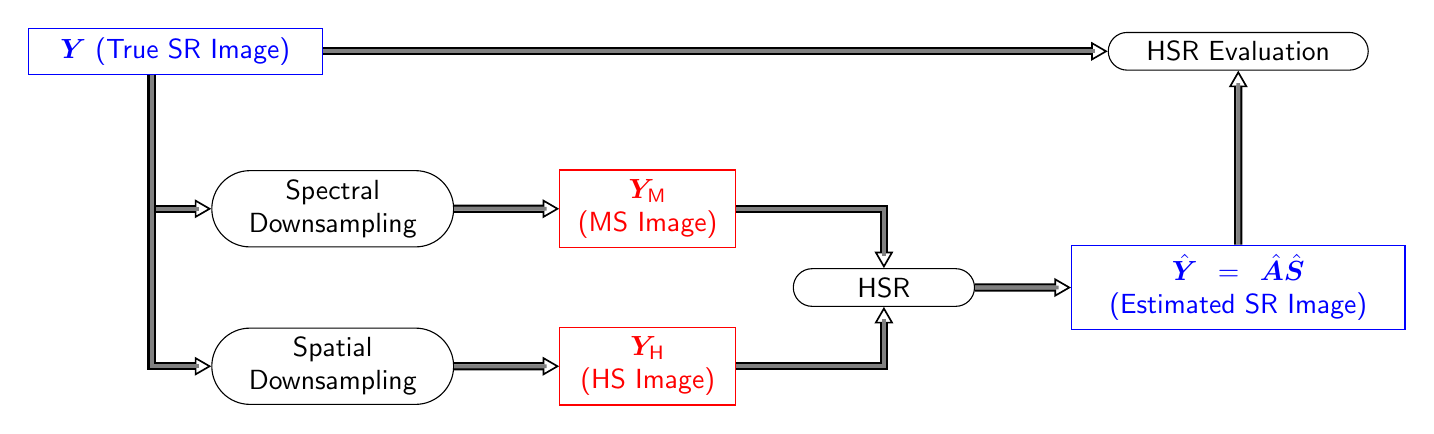
\begin{tikzpicture}
            \node at (0,0)               [xshift=   0cm,yshift=   0cm,draw                  ,text width=3.5cm,align=center, blue!100] (nSR)  {$\bm Y$ (True SR Image)};
            \node at (nSR)               [xshift= 2.0cm,yshift=  -2cm,draw,rounded rectangle,text width=2.5cm,align=center,black!100] (nF)   {Spectral\\Downsampling};
            \node at (nSR)               [xshift= 2.0cm,yshift=  -4cm,draw,rounded rectangle,text width=2.5cm,align=center,black!100] (nG)   {Spatial\\Downsampling};
            \node at (nF)                [xshift=   4cm,yshift=   0cm,draw                  ,text width=2.0cm,align=center,  red!100] (nMS)  {$\YM$\\(MS Image)};
            \node at (nG)                [xshift=   4cm,yshift=   0cm,draw                  ,text width=2.0cm,align=center,  red!100] (nHS)  {$\YH$\\(HS Image)};
            \node at ($(nHS)!0.5!(nMS)$) [xshift=   3cm,yshift=   0cm,draw,rounded rectangle,text width=2.0cm,align=center,black!100] (nHSR) {HSR};
            \node at (nHSR)              [xshift= 4.5cm,yshift=   0cm,draw                  ,text width=4cm  ,align=center, blue!100] (nSR2) {$\hat{\bm Y}=\hat{\bm A}\hat{\bm S}$\\(Estimated SR Image)};
            \node at (nSR2)              [xshift=   0cm,yshift=   3cm,draw,rounded rectangle,text width=3.0cm,align=center,black!100] (nEva) {HSR Evaluation};
            \draw[vecArrow] (nSR.-135) |- (nF)       ;
            \draw[vecArrow] (nSR.-135) |- (nG)       ;
            \draw[vecArrow] (nF.0)     to (nMS.180)  ;
            \draw[vecArrow] (nG.0)     to (nHS.180)  ;
            \draw[vecArrow] (nMS.0)    -| (nHSR)     ;
            \draw[vecArrow] (nHS.0)    -| (nHSR)     ;
            \draw[vecArrow] (nHSR.0)   to (nSR2.180) ;
            \draw[vecArrow] (nSR.0)    to (nEva.180) ;
            \draw[vecArrow] (nSR2.90)  to (nEva.-90) ;
        \end{tikzpicture}
    }
    \caption{Wald's Protocol on HS and MS images synthesis and the evaluation
             of a testing HSR method.}
    \label{fig:Walds_Protocol}
\end{figure}

Usually, to simulate real world scenario, white Gaussian noise of certain SNR
level is added linearly to the synthesized HS and MS image pair after the
downsampling processes.
The addition of noise to both images are modelled in
\eqref{eq:spatial_degradation_model} and \eqref{eq:spectral_degradation_model}.

\subsection{Spatial Degradation} \label{sec:SPATIAL_DEGRADE}
In a recent work by Wei \etal, the spatial degradation system is designed to
simulate a Gaussian low-pass filtering effect characterized by a
$11 \times 11$ mask with variance $\sigma = 1.7$.
After that the low-passed image undergoes subsampling operation of the image
on every $4$ pixels horizontally and vertically.
The spatial degradation matrix $\bm G$ of the aforementioned specification is
generated in a block circular circular block (BCCB) manner described in
\cite{FUMI}.
In this thesis we stick to the above spatial degradation settings and the
$\bm G$ matrix used is exactly the same as the one Wei \etal used in their work.
We also assume perfect prior information on $\bm G$ when we conduct HSR.

\subsection{Spectral Degradation} \label{sec:SPECTRAL_DEGRADE}
The spectral response is simulated such that the MS image simulates the optical
response of Landsat TM Sensors which capture spectral images at six wide bands
between wavelength $0.45\,\mu$m and $2.35\,\mu$m
\cite{MILITARY_UTILITY,
      LANDSAT_HANDBOOK}.
For each TM band, the observed broad band image is simulated by naively taking
the average of all band images within that broad passband.
With reference to Table \ref{table:spectral_characteristics_AVIRIS_TM}, the
first TM band can be simulated by taking the average of AVIRIS image within
$0.45\,\mu m$ and $0.52\,\mu m$, which corresponds to the $10\thtxt$ to the
$16\thtxt$ band of an AVIRIS image.
The same approach is applied to synthesize the remaining five TM band images.

\subsection{Synthetic Data Generation} \label{sec:data_gen_synt}
We generate 1000 trials per SNR level where the SR image $\bm Y$ are
synthesized using the LMM.
In each trial, the endmember matrix $\bm A$, containing $N$ spectral
signatures of spectral length $M = 224$, are randomly drawn from USGS Library
\cite{USGS}.
Also, the abundance matrix $\bm S$, containing $100 \times 100$ pixels of
uniform Dirichilet distribution, has maximum pixel purity $\rho = 0.85$.
The definition of $\rho$ is
\begin{equation}
    \rho = \underset{1 \leq i \leq L}{\max} \bm s_i\Tr \bm s_i.
\end{equation}
Note that $\bm S$ fulfills columnwise sum-to-one constraint.
In the simulation we add white Gaussian noise at three SNR levels ($40$dB,
$30$dB and $20$dB) to the HS and MS images.

\subsection{Semi-real Data Generation} \label{sec:data_gen_real}
In the two sets of semi-real data simulations we regard the real spectral
images measured by Airborne Visible/InfraRed Imaging Spectrometer (AVIRIS)
\cite{AVIRIS}
and Headwall Hyperspec-VNIR-C Imaging Sensor
\cite{NYOKOYA2016,
      HEADWALL_HYPERSPEC_VNIR_C}
as the ground truth SR images, respectively.
Both sensors are airborne type having $20$m and $2.5$m GSD, respectively.
The AVIRIS sensor takes spectral images at $224$ bands covering wavelengths
between $0.4\,\mu$m and $2.5\,\mu$m at norminally $10\,$nm intervals.
It has taken many popular spectral image datasets including Cuprite Site (whom
we use in the simulations), Indian Pines and Moffet Field.
The Hyperspec-VNIR-C sensor takes spectral images at $128$ bands covering
wavelengths between $0.363\,\mu$m and $1.018\,\mu$m at norminally $5\,$nm
intervals.
We use a big spectral image that is taken by this sensor over Chikusei region
of Japan in 2014
\cite{NYOKOYA2016}
and was later made public by Yokoya \etal.

In the first set of semi-real data simulations we fix a region of $200\times348$
pixels from the Cuprite Site dataset as the ground truth image.
We then trancate the water absorption bands and noisy bands so that only $188$
bands remain in the final SR image.
In the next set of semi-real data simulations we fix a region of
$1000 \times 1000$ pixels from the Chikusei dataset as the ground truth SR
image.
The semi-real HS and MS images are generated according to the Wald's Protocol.
Since the spectral range of the Chikusei dataset only covers four TM bands,
its simulated MS images have only four spectral bands.
Additive white Gaussian noise of desired SNR level are added to HS and MS
images as before.
Note that ground truth endmembers and abundances of the datasets are unknown
so we do not evaluate the HU performance.

Figure \ref{fig:cuprite_200x348_815nm} and \ref{fig:chikusei_1000x1000_815nm}
visualize the normalized band images of the two real datasets at $815\,$nm,
respectively.

\begin{figure}[t]
    \centering
    \subfigure[$\;$]{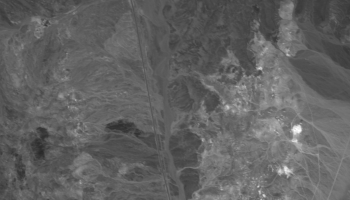
\includegraphics[width=.48\linewidth]{./fig/fig_04Expt/cuprite_200x348_815nm_normalized}\label{fig:cuprite_200x348_815nm}}
    \subfigure[$\;$]{\includegraphics[width=.48\linewidth]{./fig/fig_04Expt/cuprite_RGB}}
    \subfigure[$\;$]{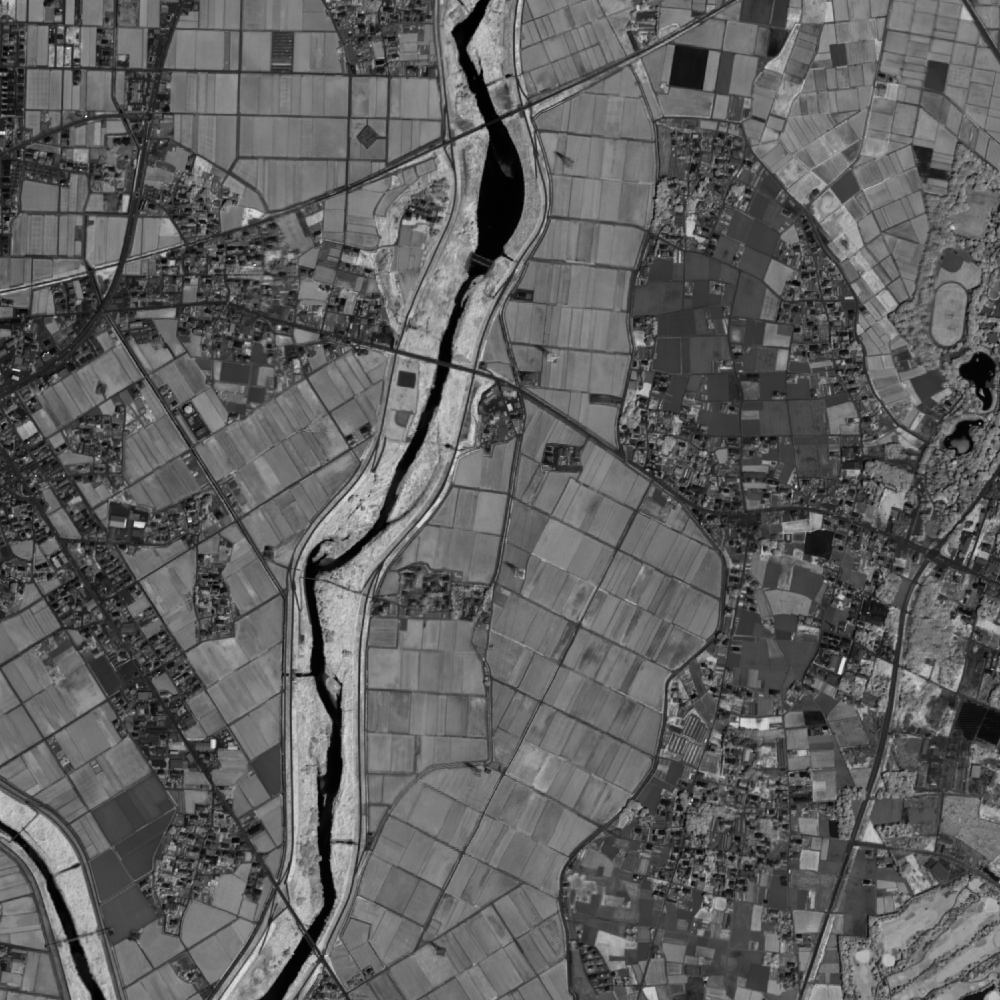
\includegraphics[width=.48\linewidth]{./fig/fig_04Expt/chikusei_1000x1000_815nm_normalized}\label{fig:chikusei_1000x1000_815nm}}
    \subfigure[$\;$]{\includegraphics[width=.48\linewidth]{./fig/fig_04Expt/chikusei_RGB}}
    \caption{$815$-nm band and the RGB image of the super-resolution images of \\
             Cuprite Site dataset ((a) and (b), $200\times348$ pixels) and
             Chikusei dataset\\((c) and (d), $1000\times1000$ pixels).}
\label{fig:real_HSI_images}
\end{figure}

\subsection{Algorithm Initialization} \label{sec:initialization}
In the general descriptions of all HSR Algorithms (ALGO, CNMF and FUMI),
they all require an initial guess on the endmember and abundance matrix pair.
Here we describe their initialization in our simulations.

The initial guess of the endmember matrix $\bm A\iter{0} \in \mathcal A$ is
obtained by Successive Projection Algorithm (SPA) \cite{SPA_CHEMOMETRICS2001,
SIGPROC_PERSP_ON_HU} followed by projection onto the feasible set $\mathcal A$.
The SPA algorithm aims at exactly indentifying the signature of all endmembers
from a HS image with the following few assumptions: 1) model order $N$ is
known; 2) HS image is noiseless; 3) LMM holds; 4) abundance sum-to-one
constraint holds; 5) for each material there exists at least a pixel that is
entirely occupied by that material (\ie pure pixel assumption holds).
When these assumptions hold, SPA can search for the endmember signatures from
the pure pixels of the HS image.
We can then further project these signatures onto $\mathcal A$ and treat them
as $\bm A\iter{0}$, \ie
\begin{equation}
    \bm A\iter{0} \gets \Pi_{\mathcal A}\left( \texttt{SPA}(\YH,N) \right).
\end{equation}
The algorithm description of SPA is shown below.
\begin{algorithm}
    \caption{Successive Projection Algorithm (SPA)}
    \begin{algorithmic}[1]
        \Require{$\bm Y$,
                 $N$.}
        \smallskip
        \State{$\bm A\iter{0} = \left[\;\right]$.}
        \smallskip
        \State{$\bm P \gets \bm I$. \; \texttt{// define projection matrix.}}
        \smallskip
        \For{$k=1,2,\cdots,N$}
            \smallskip
            \State{$\ell \gets \arg\;\underset{n\in[1,L]}{\max}
                    \Vert \bm P \bm y_n \Vert_2^2$.}
            \smallskip
            \State{$\bm \hat{\bm a}_k \gets \bm y_\ell$.}
            \smallskip
            \State{$\bm P \gets \left(\bm I - \left[ (\bm P \hat{\bm a}_k)
                    (\bm P \hat{\bm a}_k)\Tr \right]
                    / \Vert \bm P \hat{\bm a}_k \Vert_2^2 \right) \bm P$.
                   \; \texttt{// update projection matrix.}}
            \smallskip
            \State{$\bm A\iter{0} \gets \left[ \bm A\iter{0} , \hat{\bm a}_k \right]$.}
            \smallskip
        \EndFor
        \smallskip
        \Ensure{$\bm A\iter{0}$.}
    \end{algorithmic}
\end{algorithm}

In \cite{SIGPROC_PERSP_ON_HU}, the rational of SPA is found to be similar to
another endmember identification method called Successive Volume Maximization,
which is also a kind of pure-pixel-searching method relying on the pure pixel
assumption.

The initial guess of the abundance matrix is rather simple.
We naively take a constant flat map as the initial guess of the abundance map,
\ie
\begin{equation}
    \bm S\iter{0} = \frac{1}{N} \bm 1^{N \times L},
\end{equation}
which is always in the feasible sets considered in this thesis.

\subsection{Stopping Criteria of Algorithms} \label{sec:stopping_criteria}
We use the following condition to serve as all algorithms' stopping criteria.
Let us reuse the definition of $f$ in \eqref{eq:HSR_problem_CH3} and
further define $f\iter{k} \coloneqq f(\bm A\iter{k},\bm S\iter{k})$ as the
objective value at the $k\thtxt$ iteration.
We terminate any algorithms whenever the stopping criteria
\begin{equation}
    \left| \frac{f\iter{k} - f\iter{k-1}}{f\iter{k}} \right|
    \leq \delta
    \label{eq:HSR_stopping_criteria}
\end{equation}
holds, for $\delta$ being a small positive scalar.
Unless otherwise specified, we take $\delta = 10^{-4}$ in all simulations.

In ALGO, we always set $J = 1$ in all simulations.
In FUMI, stopping criteria similar to \eqref{eq:HSR_stopping_criteria} is used
in termination of both subproblems in which the threshold $\delta_S$ and
$\delta_A$ are $10^{-3}$.

\subsection{Algorithm Implementation}
\subsubsection{ALGO}
We implement ALGO to solve the HSR problem by inexact BCD purely using one of
the following FOGMs: GP, BBGP, PG, FISTA and FW.
We also tried ALGO by updating $\bm S$ subproblem with FW and $\bm A$
subproblem with FISTA.
For convenience, we call this approach "Hybrid BCD" composed of FW and FISTA.
The Hybrid BCD is designed to speed up ALGO by avoiding simplex projection in
the $\bm S$ subproblem (recall that in the HSR problem formulation of Wei
\etal in \eqref{eq:HSR_FUMI}, the constraint set of $\bm S$ is a unit simplex
for all column).
To further reduce runtime, we set $J = 1$ in all ALGO algorithm, \ie we take
a step of gradient update for each subproblem in the inexact BCD.
We expect ALGO to be fast and that ALGO by Hybrid BCD has further advantage
when model order $N$ increases under the problem formulation by Wei \etal.

In general we set $\delta = 10^{-4}$ in most simulations except that in the
simulations on Chikusei image we take $\delta = 10^{-2}$ for earlier
termination for all algorithms.

\subsubsection{FUMI}
FUMI
\cite{FUMI}
is an ADMM-based algorithm that solves problem in an alternating optimization
sense.
Based on Algorithm \ref{alg:HSR_FUMI} and its online code
\footnote{FUMI's demo code is available on https://github.com/qw245/FUMI.},
FUMI is implemented with standard stopping criteria of ADMM, \ie the primal
feasibility and dual feasibility described in
\cite{ADMM_BOYD2011}
where both primal and dual residual thresholds are set to $10^{-3}$.

\subsection{HU and HSR Quality Measures} \label{sec:Quality_Measures}
The quality measures of HU is mean-squared-error (MSE) and that of HSR are
spectral-angular-mapper (SAM) and peak-SNR (PSNR).
The algorithm efficiency is compared by their CPU runtime.
Our simulations are run on Dell Precision $7910$ with dual Intel Xeon CPU
E$5$-$2650$ v$3$ and $128$GB memory.
The definitions of the quality measures are summarized below.

\subsubsection{MSE}
The MSE measures the unmixing error of recovered endmember matrix $\bm A$
defined as
\[%\begin{equation}
    \text{MSE} = \underset{\bm \pi \in \mathcal P}{\min}
    \frac{1}{N} \sum_{k=1}^{N}
    \big|\big| \frac{\bm a_k}            {\Vert \bm a_k             \Vert_2} -
               \frac{\hat{\bm a}_{\pi_k}}{\Vert \hat{\bm a}_{\pi_k} \Vert_2}
    \big|\big|_2^2,
\]%\end{equation}
where $\mathcal P$ is the set of all permutation of $\{1,\cdots,N\}$ and
$\hat{\bm a}_k$ is the estimate of $\bm a_k$.
HU results with smaller MSE are better.

\subsubsection{RMSE}
The RMSE is a global measure between $\hat{\bm Y}$ and $\bm Y$ defined as
\[%\begin{equation}
    \text{RMSE}(\bm Y,\hat{\bm Y}) = \frac{\Vert \bm Y - \hat{\bm Y} \Vert\Fr}
                                          {\sqrt{ML}}.
\]%\end{equation}
HSR results with smaller RMSE are better.

\subsubsection{RSNR}
The RSNR is a global measure between $\hat{\bm Y}$ and $\bm Y$ defined as
\[%\begin{equation}
    \text{RSNR}(\bm Y,\hat{\bm Y}) = 10 \log_{10}\left( \frac{\Vert \bm Y \Vert\Fr^2}{\Vert \bm Y - \hat{\bm Y} \Vert\Fr^2} \right).
\]%\end{equation}
HSR results with higher RSNR are better.

\subsubsection{SAM}
We use SAM as a spectral quality measure.
The SAM between $\hat{\bm Y}$ and $\bm Y$ is defined as
\[%\begin{equation}
    \text{SAM}(\bm Y,\hat{\bm Y}) =
    \frac{1}{L} \sum_{j=1}^{L}
    \arccos
    \left( \frac{ \langle \bm y_j , \hat{\bm y}_j \rangle }
                { \Vert \bm y_j \Vert_2 \Vert \hat{\bm y}_j \Vert_2 } \right),
\]%\end{equation}
HSR results with smaller SAM are better.

\subsubsection{PSNR}
We use PSNR as a spatial quality measure.
The PSNR is defined via the mean-squared-error of each band image.
The PSNR between $\hat{\bm Y}$ and $\bm Y$ is defined as
\[%\begin{equation}
    \text{PSNR}(\bm Y , \hat{\bm Y}) =
    \frac{1}{M} \sum_{i=1}^{M} 10 \log_{10}
    \left( \frac{\text{MAX}_i^2}{\text{MSE}_i} \right),
\]%\end{equation}
where
\[
\text{MAX}_i = \max(\bm y^i)
\]
is the maximum pixel value in the $i\thtxt$ band image and
\[
\text{MSE}_i = \frac{1}{L} \Vert \bm y^i - \hat{\bm y}^i \Vert_2^2
\]
is the MSE in the $i\thtxt$ spectral band.
%where $\text{MAX}_i$ is the maximum pixel value in the $i\thtxt$ band
%image and $\text{MSE}_i = \frac{1}{L} \Vert \bm x^i - \hat{\bm x}^i \Vert_2^2$
%is the MSE in the $i\thtxt$ spectral band.
HSR results with higher PSNR are better.

\section{Experiment 1: Benchmark HSR via Exact BCD and Inexact BCD} \label{sec:expt1}
We compare the performance of HU and HSR on synthetic data using traditional
exact BCD and using inexact BCD.
Specifically, we only intensively compare FOGMs including GP, BBGP and PG.
To take part as an exact BCD, we reuse the ALGO framework by setting the
maximum number of iterations $J = 100$; to take part as an inexact BCD, we set
$J = 1$ instead.
The simulations are conducted under different environment settings including
two SNR levels and model order $N$.
\begin{table}[h]
\centering
\resizebox{0.98\linewidth}{!}{
\begin{tabular}{|c|c|c|c|c|c|c|c|c|}
\hline
\multicolumn{ 9}{|c|}{$N = 9$} \tabularnewline \hline
SNR (dB)            & Method        & MSE-en(dB)                          & MSE-ab(dB)                          & RSNR(dB)                            & RMSE(dB)                             & SAM(deg.)                          & PSNR(dB)                            & Outer Iter.           \tabularnewline \hline
%---------------------------------------------------------------------------------------------------------------------------------------------------------------------------------------------------------------------------------------------------------------------------------------------------------------------------%
\multirow{2}{*}{40} & Inex.BCD GP   & \cellcolor{red!10}{$-8.13\pm 1.16$} & \cellcolor{red!10}{$-3.66\pm 0.86$} & \cellcolor{red!10}{$19.34\pm 1.42$} & \cellcolor{red!10}{$-15.32\pm 0.65$} & \cellcolor{red!10}{$4.55\pm 0.69$} &                   {$29.21\pm 0.92$} & $1233.2   \pm 246.73$ \tabularnewline
                    & Ex.BCD:  GP   &                   {$-7.46\pm 1.1$}  &                   {$-3.4\pm 0.85$}  &                   {$19.24\pm 1.72$} &                   {$-15.27\pm 0.89$} &                   {$4.68\pm 0.76$} & \cellcolor{red!10}{$29.24\pm 1.34$} & $298.53   \pm 72.13$  \tabularnewline \hline
\multirow{2}{*}{20} & Inex.BCD GP   & \cellcolor{red!10}{$-6.75\pm 0.84$} & \cellcolor{red!10}{$-2.73\pm 0.46$} & \cellcolor{red!10}{$17.13\pm 0.87$} & \cellcolor{red!10}{$-14.21\pm 0.58$} & \cellcolor{red!10}{$6.69\pm 0.57$} & \cellcolor{red!10}{$23.07\pm 0.67$} & $165.91   \pm 21.13$  \tabularnewline
                    & Ex.BCD:  GP   &                   {$-5.1\pm 0.62$}  &                   {$-2.4\pm 0.43$}  &                   {$16.27\pm 0.69$} &                   {$-13.78\pm 0.6$}  &                   {$8.17\pm 0.51$} &                   {$22.21\pm 0.97$} & $52.73    \pm 6.87$   \tabularnewline \hline \hline
%---------------------------------------------------------------------------------------------------------------------------------------------------------------------------------------------------------------------------------------------------------------------------------------------------------------------------%
\multirow{2}{*}{40} & Inex.BCD BBGP & \cellcolor{red!10}{$-8.24\pm 1.12$} & \cellcolor{red!10}{$-3.62\pm 0.83$} & \cellcolor{red!10}{$19.57\pm 1.41$} & \cellcolor{red!10}{$-15.43\pm 0.75$} & \cellcolor{red!10}{$4.38\pm 0.66$} & \cellcolor{red!10}{$29.38\pm 0.95$} & $1303.63  \pm 238.66$ \tabularnewline
                    & Ex.BCD:  BBGP &                   {$-7.47\pm 1.1$}  &                   {$-3.43\pm 0.83$} &                   {$19.36\pm 1.67$} &                   {$-15.33\pm 0.89$} &                   {$4.66\pm 0.75$} &                   {$29.32\pm 1.3$}  & $297.17   \pm 70.9$   \tabularnewline \hline
\multirow{2}{*}{20} & Inex.BCD BBGP & \cellcolor{red!10}{$-6.88\pm 0.79$} & \cellcolor{red!10}{$-2.45\pm 0.43$} & \cellcolor{red!10}{$16.98\pm 0.85$} & \cellcolor{red!10}{$-14.13\pm 0.6$}  & \cellcolor{red!10}{$6.79\pm 0.57$} & \cellcolor{red!10}{$22.93\pm 0.73$} & $245.73   \pm 33.62$  \tabularnewline
                    & Ex.BCD:  BBGP &                   {$-5.26\pm 0.62$} &                   {$-2.4\pm 0.42$}  &                   {$16.38\pm 0.7$}  &                   {$-13.84\pm 0.59$} &                   {$8.03\pm 0.5$}  &                   {$22.33\pm 0.96$} & $57.3     \pm 6.19$   \tabularnewline \hline \hline
%---------------------------------------------------------------------------------------------------------------------------------------------------------------------------------------------------------------------------------------------------------------------------------------------------------------------------%
\multirow{2}{*}{40} & Inex.BCD PG   & \cellcolor{red!10}{$-8.23\pm 1.11$} &                   {$-3.98\pm 0.68$} & \cellcolor{red!10}{$21.53\pm 1.72$} & \cellcolor{red!10}{$-16.41\pm 0.62$} & \cellcolor{red!10}{$3.82\pm 0.67$} &                   {$30.69\pm 1.29$} & $3062.73  \pm 282.5$  \tabularnewline
                    & Ex.BCD:  PG   &                   {$-7.75\pm 1.06$} & \cellcolor{red!10}{$-4.01\pm 0.77$} &                   {$21.16\pm 1.82$} &                   {$-16.23\pm 0.7$}  &                   {$3.92\pm 0.76$} & \cellcolor{red!10}{$31\pm 1.44$}    & $324.91   \pm 82.85$  \tabularnewline \hline
\multirow{2}{*}{20} & Inex.BCD PG   & \cellcolor{red!10}{$-6.65\pm 0.71$} & \cellcolor{red!10}{$-2.97\pm 0.44$} & \cellcolor{red!10}{$17.42\pm 0.75$} & \cellcolor{red!10}{$-14.36\pm 0.54$} & \cellcolor{red!10}{$6.56\pm 0.57$} & \cellcolor{red!10}{$23.31\pm 0.85$} & $626.33   \pm 58.86$  \tabularnewline
                    & Ex.BCD:  PG   &                   {$-5.6\pm 0.66$}  &                   {$-2.81\pm 0.42$} &                   {$16.95\pm 0.77$} &                   {$-14.12\pm 0.58$} &                   {$7.25\pm 0.51$} &                   {$22.93\pm 0.87$} & $70.86    \pm 5.4$    \tabularnewline \hline
%---------------------------------------------------------------------------------------------------------------------------------------------------------------------------------------------------------------------------------------------------------------------------------------------------------------------------%
\end{tabular}
}
\caption{Average HSR performance on synthetic data by using Exact BCD and
         Inexact BCD. FOGMs include GP, BBGP and PG. Model order $N = 9$.
         Pixel number $L = 100 \times 100$.}
\label{table:ALGO_1_vs_100_it_SYNT_MO9}
\end{table}

\begin{table}[h]
\centering
\resizebox{0.98\linewidth}{!}{
\begin{tabular}{|c|c|c|c|c|c|c|}
\hline
\multicolumn{ 7}{|c|}{$N = 16$} \tabularnewline \hline
SNR (dB)            & Method        & RSNR(dB)                            & RMSE(dB)                             & SAM(deg.)                          & PSNR(dB)                            & Outer Iter.           \tabularnewline \hline
%-----------------------------------------------------------------------------------------------------------------------------------------------------------------------------------------------------------------------------------------------%
\multirow{2}{*}{40} & Inex.BCD GP   & \cellcolor{red!10}{$35.53\pm 0.15$} & \cellcolor{red!10}{$-23.18\pm 0.08$} & \cellcolor{red!10}{$0.88\pm 0.01$} & \cellcolor{red!10}{$44.27\pm 0.13$} & $984.38   \pm 50.37$  \tabularnewline
                    & Ex.BCD:  GP   &                   {$32.74\pm 0.32$} &                   {$-21.78\pm 0.16$} &                   {$1.19\pm 0.03$} &                   {$42.06\pm 0.22$} & $243.32   \pm 14.47$  \tabularnewline \hline
\multirow{2}{*}{20} & Inex.BCD GP   & \cellcolor{red!10}{$21.19\pm 0.08$} & \cellcolor{red!10}{$-16.01\pm 0.04$} & \cellcolor{red!10}{$4.27\pm 0.05$} & \cellcolor{red!10}{$28.77\pm 0.09$} & $195.02   \pm 10.27$  \tabularnewline
                    & Ex.BCD:  GP   &                   {$17.7\pm 0.27$}  &                   {$-14.27\pm 0.13$} &                   {$6.87\pm 0.25$} &                   {$25.28\pm 0.26$} & $54.99    \pm 4.19$   \tabularnewline \hline \hline
%-----------------------------------------------------------------------------------------------------------------------------------------------------------------------------------------------------------------------------------------------%
\multirow{2}{*}{40} & Inex.BCD BBGP & \cellcolor{red!10}{$35.69\pm 0.09$} & \cellcolor{red!10}{$-23.26\pm 0.05$} & \cellcolor{red!10}{$0.86\pm 0.01$} & \cellcolor{red!10}{$44.43\pm 0.08$} & $966.22   \pm 122.08$ \tabularnewline
                    & Ex.BCD:  BBGP &                   {$32.7\pm 0.33$}  &                   {$-21.77\pm 0.16$} &                   {$1.19\pm 0.03$} &                   {$42.06\pm 0.21$} & $248.25   \pm 16.46$  \tabularnewline \hline
\multirow{2}{*}{20} & Inex.BCD BBGP & \cellcolor{red!10}{$21.3\pm 0.07$}  & \cellcolor{red!10}{$-16.07\pm 0.03$} & \cellcolor{red!10}{$4.2\pm 0.04$}  & \cellcolor{red!10}{$28.9\pm 0.08$}  & $207.79   \pm 19.76$  \tabularnewline
                    & Ex.BCD:  BBGP &                   {$18.19\pm 0.19$} &                   {$-14.51\pm 0.09$} &                   {$6.44\pm 0.17$} &                   {$25.75\pm 0.18$} & $63.25    \pm 4.26$   \tabularnewline \hline \hline
%-----------------------------------------------------------------------------------------------------------------------------------------------------------------------------------------------------------------------------------------------%
\multirow{2}{*}{40} & Inex.BCD PG   & \cellcolor{red!10}{$35.93\pm 0.03$} & \cellcolor{red!10}{$-23.38\pm 0.02$} & \cellcolor{red!10}{$0.84\pm 0$}    & \cellcolor{red!10}{$44.77\pm 0.04$} & $2516.63  \pm 98.48$  \tabularnewline
                    & Ex.BCD:  PG   &                   {$35.29\pm 0.12$} &                   {$-23.06\pm 0.06$} &                   {$0.91\pm 0.01$} &                   {$44.08\pm 0.1$}  & $269.25   \pm 20.68$  \tabularnewline \hline
\multirow{2}{*}{20} & Inex.BCD PG   & \cellcolor{red!10}{$22.19\pm 0.05$} & \cellcolor{red!10}{$-16.51\pm 0.02$} & \cellcolor{red!10}{$3.66\pm 0.02$} & \cellcolor{red!10}{$29.88\pm 0.05$} & $475.63   \pm 25.43$  \tabularnewline
                    & Ex.BCD:  PG   &                   {$20.19\pm 0.08$} &                   {$-15.51\pm 0.04$} &                   {$4.95\pm 0.05$} &                   {$27.72\pm 0.09$} & $80.46    \pm 4.28$   \tabularnewline \hline
%-----------------------------------------------------------------------------------------------------------------------------------------------------------------------------------------------------------------------------------------------%
\end{tabular}
}
\caption{Average HSR performance on Cuprite dataset by using Exact BCD and
         Inexact BCD. FOGMs include GP, BBGP and PG. Model order $N = 16$.
         Pixel number $L = 200 \times 348$.}
\label{table:ALGO_1_vs_100_it_REAL_CUPRITE_MO16}
\end{table}

\newpage
In the first part, we conduct synthetic simulation taking model order $N = 9$.
The HU and HSR results are the average of 1000 trials of synthetic data
generated according to the description in Section \ref{sec:data_gen_synt}.
In the second part we set $N = 16$ in the semi-real Cuprite dataset simulation.
The HSR results are the average of 100 trials of semi-real data generated
according to the description in Section \ref{sec:data_gen_real}.
The results are shown in Table \ref{table:ALGO_1_vs_100_it_SYNT_MO9} and
\ref{table:ALGO_1_vs_100_it_REAL_CUPRITE_MO16}, respectively.

We highlight the better results in Table \ref{table:ALGO_1_vs_100_it_SYNT_MO9}
and \ref{table:ALGO_1_vs_100_it_REAL_CUPRITE_MO16} where we can see the
highlighted performance mostly belong to inexact methods.
Table \ref{table:ALGO_1_vs_100_it_REAL_CUPRITE_MO16} also shows that inexact
BCD methods can even outperform the exact BCD methods roughly by a $2$dB
improvement.

Regarding the algorithm efficiency, it can be compared by counting on the 
total number of gradient updates ($J\times\text{Outer Iter.}$) of the
algorithms.
From the results above, we may conclude that ALGO using inexact BCD is
advantageous because it reduces the computation and maintains a comparable or
improved performance.
In most cases, 

%\section{Experiment 2: Benchmark HSR via ALGO using Different FOGMs}
\section{Experiment 2: Benchmark HSR via ALGO using FOGMs}
We compare the HU and HSR performance of ALGO using a range of FOGMs by two
sets of simulations.
The first one is a synthetic data simulation while the second one is a
semi-real Cuprite dataset simulation.
Our interest focuses on \textit{inexact} BCD since they have generally better
performance and higher efficiency as demonstrated in Section \ref{sec:expt1}.
Since there are too many quality measures, here we only compare the algorithms
by MSE-en (for benchmarking HU), SAM and PSNR (for benchmarking HSR spectrally
and spatially, respectively).
The algorithm runtime is also counted to compare their efficiency.
\begin{table}[h]
\centering
\resizebox{0.80\linewidth}{!}{
\begin{tabular}{|c|c|c|c|c|c|}
\hline
\multicolumn{ 6}{|c|}{$N = 9$} \tabularnewline \hline
SNR (dB)            & ALGO   & MSE-en(dB)                          & SAM(deg.)                          & PSNR(dB)                            & Time(sec.)                          \tabularnewline \hline
%---------------------------------------------------------------------------------------------------------------------------------------------------------------------------------------------------------------%
\multirow{5}{*}{40} & GP     &                   {$-8.13\pm 1.16$} &                   {$4.55\pm 0.69$} &                   {$29.21\pm 0.92$} &                   {$15.82\pm 4.55$} \tabularnewline
                    & BBGP   & \cellcolor{red!10}{$-8.24\pm 1.12$} &                   {$4.38\pm 0.66$} &                   {$29.38\pm 0.95$} &                   {$18.06\pm 4.82$} \tabularnewline
                    & PG     &                   {$-8.23\pm 1.11$} &                   {$3.82\pm 0.67$} &                   {$30.69\pm 1.29$} &                   {$26.41\pm 5.75$} \tabularnewline
                    & FISTA  &                   {$-7.99\pm 1.17$} & \cellcolor{red!10}{$3.41\pm 0.94$} & \cellcolor{red!10}{$32.48\pm 2.3$}  & \cellcolor{red!10}{$5.36\pm 1.3$}   \tabularnewline
                    & FW     &                   {$-8.13\pm 0.99$} &                   {$4.9\pm 0.68$}  &                   {$28.6\pm 0.91$}  &                   {$14.12\pm 3.76$} \tabularnewline \hline \hline
%---------------------------------------------------------------------------------------------------------------------------------------------------------------------------------------------------------------%
\multirow{5}{*}{30} & GP     &                   {$-8.02\pm 1.16$} &                   {$5.03\pm 0.67$} &                   {$26.81\pm 0.73$} &                   {$6.21\pm 1.66$}  \tabularnewline
                    & BBGP   & \cellcolor{red!10}{$-8.12\pm 1.11$} &                   {$4.9\pm 0.63$}  &                   {$26.93\pm 0.78$} &                   {$7.91\pm 2.01$}  \tabularnewline
                    & PG     &                   {$-8.04\pm 1.06$} &                   {$4.48\pm 0.6$}  &                   {$27.88\pm 1.04$} &                   {$12.94\pm 2.81$} \tabularnewline
                    & FISTA  &                   {$-7.6\pm 1.08$}  & \cellcolor{red!10}{$4.24\pm 0.79$} & \cellcolor{red!10}{$28.84\pm 1.6$}  & \cellcolor{red!10}{$3.02\pm 0.67$}  \tabularnewline
                    & FW     &                   {$-7.98\pm 1.04$} &                   {$5.26\pm 0.67$} &                   {$26.62\pm 0.78$} &                   {$6.25\pm 1.66$}  \tabularnewline \hline
%---------------------------------------------------------------------------------------------------------------------------------------------------------------------------------------------------------------%
\multicolumn{ 6}{|c|}{$N =16$} \tabularnewline \hline
SNR (dB)            & ALGO   & MSE-en(dB)                          & SAM(deg.)                          & PSNR(dB)                            & Time(sec.)                          \tabularnewline \hline
%---------------------------------------------------------------------------------------------------------------------------------------------------------------------------------------------------------------%
\multirow{5}{*}{40} & GP     &                   {$-7.69\pm 0.6$}  &                   {$4.22\pm 0.4$}  &                   {$28.9\pm 0.56$}  &                   {$13.5\pm 5.85$}  \tabularnewline
                    & BBGP   &                   {$-7.73\pm 0.58$} &                   {$4.1\pm 0.36$}  &                   {$29.13\pm 0.58$} &                   {$17.11\pm 7.58$} \tabularnewline
                    & PG     &                   {$-7.93\pm 0.64$} &                   {$3.58\pm 0.37$} &                   {$30.57\pm 0.83$} &                   {$36.28\pm 14.9$} \tabularnewline
                    & FISTA  & \cellcolor{red!10}{$-7.94\pm 0.67$} & \cellcolor{red!10}{$3.07\pm 0.54$} & \cellcolor{red!10}{$32.22\pm 1.55$} & \cellcolor{red!10}{$6.46\pm 2.86$}  \tabularnewline
                    & FW     &                   {$-7.43\pm 0.53$} &                   {$4.7\pm 0.37$}  &                   {$27.95\pm 0.51$} &                   {$10.25\pm 4.93$} \tabularnewline \hline \hline
%---------------------------------------------------------------------------------------------------------------------------------------------------------------------------------------------------------------%
\multirow{5}{*}{30} & GP     &                   {$-7.48\pm 0.56$} &                   {$4.58\pm 0.38$} &                   {$26.79\pm 0.46$} &                   {$6.87\pm 3.2$}   \tabularnewline
                    & BBGP   &                   {$-7.5\pm 0.54$}  &                   {$4.51\pm 0.34$} &                   {$26.89\pm 0.48$} &                   {$8.72\pm 4.06$}  \tabularnewline
                    & PG     & \cellcolor{red!10}{$-7.61\pm 0.54$} &                   {$4.18\pm 0.31$} &                   {$27.81\pm 0.64$} &                   {$15.95\pm 7.2$}  \tabularnewline
                    & FISTA  &                   {$-7.28\pm 0.56$} & \cellcolor{red!10}{$3.93\pm 0.48$} & \cellcolor{red!10}{$28.49\pm 1.17$} & \cellcolor{red!10}{$4.41\pm 2.14$}  \tabularnewline
                    & FW     &                   {$-7.27\pm 0.5$}  &                   {$5.02\pm 0.36$} &                   {$26.05\pm 0.44$} &                   {$4.43\pm 2.2$}   \tabularnewline \hline
%---------------------------------------------------------------------------------------------------------------------------------------------------------------------------------------------------------------%
\end{tabular}
}
\caption{Average HSR performance on synthetic data by Inexact BCD using a
         range of FOGMs. Pixel number $L = 100 \times 100$.}
\label{table:ALGO_GP_BB_PG_FISTA_FW_vs_SYNT_MO9_MO16}
\end{table}

\begin{table}[h]
\centering
\resizebox{0.75\linewidth}{!}{
\begin{tabular}{|c|c|c|c|c|}
\hline
\multicolumn{ 5}{|c|}{$N = 9$} \tabularnewline \hline
SNR (dB)            & ALGO   & SAM(deg.)                          & PSNR(dB)                            & Time(sec.)                            \tabularnewline \hline
%----------------------------------------------------------------------------------------------------------------------------------------------------------------------------%
\multirow{5}{*}{40} & GP     &                   {$0.99\pm 0.02$} &                   {$43.24\pm 0.14$} &                   {$39.95\pm 3.45$}   \tabularnewline
                    & BBGP   &                   {$0.94\pm 0.02$} &                   {$43.78\pm 0.13$} &                   {$37.19\pm 5.91$}   \tabularnewline
                    & PG     & \cellcolor{red!10}{$0.88\pm 0$}    & \cellcolor{red!10}{$44.37\pm 0.03$} &                   {$61.84\pm 5.32$}   \tabularnewline
                    & FISTA  &                   {$1.17\pm 0.03$} &                   {$42.13\pm 0.21$} & \cellcolor{red!10}{$18.69\pm 1.91$}   \tabularnewline
                    & FW     &                   {$1.08\pm 0.02$} &                   {$42.64\pm 0.11$} &                   {$24.56\pm 3.11$}   \tabularnewline \hline \hline
%----------------------------------------------------------------------------------------------------------------------------------------------------------------------------%
\multirow{5}{*}{30} & GP     &                   {$1.76\pm 0.05$} &                   {$36.92\pm 0.2$}  &                   {$16.13\pm 1.73$}   \tabularnewline
                    & BBGP   &                   {$1.67\pm 0.06$} &                   {$37.28\pm 0.24$} &                   {$17.44\pm 2.26$}   \tabularnewline
                    & PG     & \cellcolor{red!10}{$1.56\pm 0.03$} & \cellcolor{red!10}{$37.82\pm 0.12$} &                   {$34.59\pm 3.21$}   \tabularnewline
                    & FISTA  &                   {$2.55\pm 0.22$} &                   {$34.61\pm 0.49$} & \cellcolor{red!10}{$9.05\pm 1.02$}    \tabularnewline
                    & FW     &                   {$1.87\pm 0.05$} &                   {$36.49\pm 0.16$} &                   {$12.03\pm 1.46$}   \tabularnewline \hline \hline
%----------------------------------------------------------------------------------------------------------------------------------------------------------------------------%
\multicolumn{ 5}{|c|}{$N =16$} \tabularnewline \hline
SNR (dB)            & ALGO   & SAM(deg.)                          & PSNR(dB)                            & Time(sec.)                            \tabularnewline \hline
%----------------------------------------------------------------------------------------------------------------------------------------------------------------------------%
\multirow{5}{*}{40} & GP     &                   {$0.88\pm 0.01$} &                   {$44.27\pm 0.13$} &                   {$65.95\pm 6.26$}   \tabularnewline
                    & BBGP   &                   {$0.86\pm 0.01$} &                   {$44.43\pm 0.08$} &                   {$68.31\pm 10.27$}  \tabularnewline
                    & PG     & \cellcolor{red!10}{$0.84\pm 0$}    & \cellcolor{red!10}{$44.77\pm 0.04$} &                   {$129.73\pm 15.25$} \tabularnewline
                    & FISTA  &                   {$1\pm 0.02$}    &                   {$43.38\pm 0.11$} & \cellcolor{red!10}{$26.3\pm 2.98$}    \tabularnewline
                    & FW     &                   {$1.03\pm 0.02$} &                   {$43\pm 0.13$}    &                   {$39.62\pm 4.06$}   \tabularnewline \hline \hline
%----------------------------------------------------------------------------------------------------------------------------------------------------------------------------%
\multirow{5}{*}{30} & GP     &                   {$1.57\pm 0.02$} &                   {$37.73\pm 0.11$} &                   {$26.81\pm 2.6$}    \tabularnewline
                    & BBGP   &                   {$1.56\pm 0.02$} &                   {$37.76\pm 0.11$} &                   {$27.85\pm 3.95$}   \tabularnewline
                    & PG     & \cellcolor{red!10}{$1.51\pm 0.01$} & \cellcolor{red!10}{$38.03\pm 0.07$} &                   {$56.64\pm 5.88$}   \tabularnewline
                    & FISTA  &                   {$2.04\pm 0.05$} &                   {$35.85\pm 0.17$} &                   {$17.22\pm 1.81$}   \tabularnewline
                    & FW     &                   {$1.82\pm 0.03$} &                   {$36.63\pm 0.12$} & \cellcolor{red!10}{$14.2\pm 1.4$}     \tabularnewline \hline
%----------------------------------------------------------------------------------------------------------------------------------------------------------------------------%
\end{tabular}
}
\caption{Average HSR performance on Cuprite dataset by Inexact BCD using a
         range of FOGMs. Pixel number $L = 200 \times 348$.}
\label{table:ALGO_GP_BB_PG_FISTA_FW_vs_REAL_CUPRITE_MO9_MO16}
\end{table}

Similar as before, we highlight the best results in Table
\ref{table:ALGO_GP_BB_PG_FISTA_FW_vs_SYNT_MO9_MO16} and
\ref{table:ALGO_GP_BB_PG_FISTA_FW_vs_REAL_CUPRITE_MO9_MO16}.
Table \ref{table:ALGO_GP_BB_PG_FISTA_FW_vs_SYNT_MO9_MO16} shows that FISTA
ususally has better HSR performance than ALGO using other FOGMs).
However the HU performance is roughly the same as others (generally
worse than others by no more than $0.5$dB).
We are more interested in the runtime performance of ALGO using FISTA because
it requires significantly fewer computation time than other algorithms. 

When we benchmark the algorithms using semi-real Cuprite dataset, as shown in
Table \ref{table:ALGO_GP_BB_PG_FISTA_FW_vs_REAL_CUPRITE_MO9_MO16}, we see that
ALGO using PG has the best HSR performance although it requires the most
computation time.

Overall, PG and FISTA generally have better performance in terms of HSR
quality and runtime, respectively.
The competitiveness of runtime of FISTA supports our expectation on its
convergence rate $\mathcal O(1/k^2)$ stated in Section \ref{sec:QP_by_FISTA},
although we are now in the context of inexact BCD.

FW is also almost the second fastest algorithm.
A major reason goes to its projection-free nature described in Section
\ref{sec:QP_by_FW} whom we may predict that the projection operation becomes
more expensive when model order $N$ and pixel number $L$ increase.

From the above results, we may conclude that ALGO using PG and FISTA generally
perform better in terms of HU and HSR performance while ALGO using FISTA and
FW is faster.
From now on we focus on ALGO using the aforementioned three FOGMs.

\newpage
\section{Experiment 3: Benchmark HSR via ALGO and FUMI}
We compare the performance of ALGO and FUMI in three parts.
First we use synthetic data simulation to compare their HU and HSR
performance.
After that we use semi-real data generated from the Cuprite dataset and the
Chikusei dataset to compare their HSR performance.

\subsection{Results on Synthetic Data}
We apply FUMI and ALGO to synthetic data.
\begin{table}[h]
\centering
\resizebox{0.85\linewidth}{!}{
\begin{threeparttable}
\begin{tabular}{|c|c|c|c|c|c|}
\hline
\multicolumn{ 6}{|c|}{$N = 9$} \tabularnewline \hline
SNR (dB)            & Method                 & MSE-en(dB)                           & SAM(deg.)                           & PSNR(dB)                             & Time(sec.)                              \tabularnewline \hline
%--------------------------------------------------------------------------------------------------------------------------------------------------------------------------------------------------------------------------------%
\multirow{5}{*}{40} & FUMI                   &                    {$-7.37\pm 1.1$}  &                    {$3.63\pm 0.76$} &                    {$31.37\pm 1.59$} &                    {$411.23\pm 119.49$} \tabularnewline
                    & ALGO: PG               & \cellcolor{red! 10}{$-8.23\pm 1.11$} &                    {$3.82\pm 0.67$} &                    {$30.69\pm 1.29$} &                    {$26.41\pm 5.75$}    \tabularnewline
                    & ALGO: FISTA            &                    {$-7.99\pm 1.17$} & \cellcolor{red! 10}{$3.41\pm 0.94$} & \cellcolor{red! 10}{$32.48\pm 2.3$}  & \cellcolor{red! 10}{$5.36\pm 1.3$}      \tabularnewline
                    & ALGO: FW               &                    {$-8.13\pm 0.99$} &                    {$4.9\pm 0.68$}  &                    {$28.6\pm 0.91$}  &                    {$14.12\pm 3.76$}    \tabularnewline
                    & ALGO: Hybrid \tnote{1} &                    {$-6.94\pm 1.12$} &                    {$3.99\pm 0.79$} &                    {$31.22\pm 1.64$} &                    {$7.75\pm 1.54$}     \tabularnewline \hline \hline
%--------------------------------------------------------------------------------------------------------------------------------------------------------------------------------------------------------------------------------%
\multirow{5}{*}{30} & FUMI                   &                    {$-6.99\pm 1.03$} &                    {$4.39\pm 0.62$} &                    {$28.37\pm 1.22$} &                    {$293.29\pm 79.24$}  \tabularnewline
                    & ALGO: PG               & \cellcolor{red! 10}{$-8.04\pm 1.06$} &                    {$4.48\pm 0.6$}  &                    {$27.88\pm 1.04$} &                    {$12.94\pm 2.81$}    \tabularnewline
                    & ALGO: FISTA            &                    {$-7.6\pm 1.08$}  & \cellcolor{red! 10}{$4.24\pm 0.79$} & \cellcolor{red! 10}{$28.84\pm 1.6$}  & \cellcolor{red! 10}{$3.02\pm 0.67$}     \tabularnewline
                    & ALGO: FW               &                    {$-7.98\pm 1.04$} &                    {$5.26\pm 0.67$} &                    {$26.62\pm 0.78$} &                    {$6.25\pm 1.66$}     \tabularnewline
                    & ALGO: Hybrid \tnote{1} &                    {$-6.92\pm 1.1$}  &                    {$4.68\pm 0.7$}  &                    {$28.01\pm 1.14$} &                    {$3.59\pm 0.95$}     \tabularnewline \hline \hline
%--------------------------------------------------------------------------------------------------------------------------------------------------------------------------------------------------------------------------------%
\multirow{5}{*}{20} & FUMI                   &                    {$-4.74\pm 0.59$} &                    {$8.27\pm 0.41$} &                    {$22.09\pm 0.99$} &                    {$248.53\pm 67.97$}  \tabularnewline
                    & ALGO: PG               &                    {$-6.65\pm 0.71$} & \cellcolor{red! 10}{$6.56\pm 0.57$} & \cellcolor{red! 10}{$23.31\pm 0.85$} &                    {$5.94\pm 1.25$}     \tabularnewline
                    & ALGO: FISTA            &                    {$-5.63\pm 0.71$} &                    {$7.16\pm 0.52$} &                    {$23.12\pm 1.02$} &                    {$2.11\pm 0.42$}     \tabularnewline
                    & ALGO: FW               & \cellcolor{red! 10}{$-7\pm 0.79$}    &                    {$6.83\pm 0.59$} &                    {$22.99\pm 0.75$} &                    {$2.78\pm 0.66$}     \tabularnewline
                    & ALGO: Hybrid \tnote{1} &                    {$-5.48\pm 0.72$} &                    {$7.19\pm 0.52$} &                    {$23.02\pm 0.88$} & \cellcolor{red! 10}{$1.3\pm 0.43$}      \tabularnewline \hline \hline
%--------------------------------------------------------------------------------------------------------------------------------------------------------------------------------------------------------------------------------%
\multicolumn{ 6}{|c|}{$N =16$} \tabularnewline \hline
SNR (dB)            & Method                 & MSE-en(dB)                           & SAM(deg.)                           & PSNR(dB)                             & Time(sec.)                              \tabularnewline \hline
%--------------------------------------------------------------------------------------------------------------------------------------------------------------------------------------------------------------------------------%
\multirow{5}{*}{40} & FUMI                   &                    {$-6.47\pm 0.63$} &                    {$4.19\pm 0.4$}  &                    {$28.88\pm 0.71$} &                    {$556.08\pm 146.21$} \tabularnewline
                    & ALGO: PG               &                    {$-7.93\pm 0.64$} &                    {$3.58\pm 0.37$} &                    {$30.57\pm 0.83$} &                    {$36.28\pm 14.9$}    \tabularnewline
                    & ALGO: FISTA            & \cellcolor{red! 10}{$-7.94\pm 0.67$} & \cellcolor{red! 10}{$3.07\pm 0.54$} & \cellcolor{red! 10}{$32.22\pm 1.55$} &                    {$6.46\pm 2.86$}     \tabularnewline
                    & ALGO: FW               &                    {$-7.43\pm 0.53$} &                    {$4.7\pm 0.37$}  &                    {$27.95\pm 0.51$} &                    {$10.25\pm 4.93$}    \tabularnewline
                    & ALGO: Hybrid \tnote{1} &                    {$-6.96\pm 0.61$} &                    {$4.03\pm 0.45$} &                    {$30.24\pm 0.89$} & \cellcolor{red! 10}{$5.7\pm 1.43$}      \tabularnewline \hline \hline
%--------------------------------------------------------------------------------------------------------------------------------------------------------------------------------------------------------------------------------%
\multirow{5}{*}{30} & FUMI                   &                    {$-6.08\pm 0.52$} &                    {$4.6\pm 0.32$}  &                    {$26.75\pm 0.56$} &                    {$366.32\pm 108.43$} \tabularnewline
                    & ALGO: PG               & \cellcolor{red! 10}{$-7.61\pm 0.54$} &                    {$4.18\pm 0.31$} &                    {$27.81\pm 0.64$} &                    {$15.95\pm 7.2$}     \tabularnewline
                    & ALGO: FISTA            &                    {$-7.28\pm 0.56$} & \cellcolor{red! 10}{$3.93\pm 0.48$} & \cellcolor{red! 10}{$28.49\pm 1.17$} &                    {$4.41\pm 2.14$}     \tabularnewline
                    & ALGO: FW               &                    {$-7.27\pm 0.5$}  &                    {$5.02\pm 0.36$} &                    {$26.05\pm 0.44$} &                    {$4.43\pm 2.2$}      \tabularnewline
                    & ALGO: Hybrid \tnote{1} &                    {$-6.77\pm 0.56$} &                    {$4.67\pm 0.39$} &                    {$27.14\pm 0.72$} & \cellcolor{red! 10}{$2.82\pm 0.78$}     \tabularnewline \hline \hline
%--------------------------------------------------------------------------------------------------------------------------------------------------------------------------------------------------------------------------------%
\multirow{5}{*}{20} & FUMI                   &                    {$-3.93\pm 0.31$} &                    {$9.04\pm 0.37$} &                    {$20.67\pm 0.63$} &                    {$512.21\pm 167.4$}  \tabularnewline
                    & ALGO: PG               &                    {$-6.1\pm 0.34$}  & \cellcolor{red! 10}{$5.97\pm 0.32$} & \cellcolor{red! 10}{$23.48\pm 0.54$} &                    {$9.99\pm 4.4$}      \tabularnewline
                    & ALGO: FISTA            &                    {$-4.81\pm 0.33$} &                    {$7.87\pm 0.26$} &                    {$21.82\pm 0.6$}  &                    {$3.57\pm 1.66$}     \tabularnewline
                    & ALGO: FW               & \cellcolor{red! 10}{$-6.21\pm 0.39$} &                    {$7.1\pm 0.29$}  &                    {$22.14\pm 0.43$} &                    {$2.71\pm 1.42$}     \tabularnewline
                    & ALGO: Hybrid \tnote{1} &                    {$-4.82\pm 0.31$} &                    {$8.07\pm 0.24$} &                    {$21.59\pm 0.58$} & \cellcolor{red! 10}{$1.62\pm 0.48$}     \tabularnewline \hline
%--------------------------------------------------------------------------------------------------------------------------------------------------------------------------------------------------------------------------------%
\end{tabular}
\begin{tablenotes}
\item[1] Hybrid update on $\bm S$ by FW and on $\bm A$ by FISTA.
\end{tablenotes}
\end{threeparttable}
}
\caption{HU and HSR performance on synthetic data by FUMI and ALGO.
         $L = 100 \times 100$. Highlighted results indicate they are the best
         under the setting.}
\label{table:ALGO_vs_FUMI_SYNT_MO9}
\end{table}

In Table \ref{table:ALGO_vs_FUMI_SYNT_MO9} we see that ALGO generally has a
comparable or better performance than FUMI does.
The best HSR performance roughly goes to ALGO using PG and FISTA.
In all case, the runtime required by ALGO is significantly fewer than that 
required by FUMI.
Among the ALGO algorithms, FISTA is almost the fastest when model order is
small ($N = 9$) while that of Hybrid BCD is the fastest when model order is
large ($N = 16$).

%\newpage
\subsection{Results on Semi-real Cuprite Dataset}
We apply FUMI and ALGO to the semi-real Cuprite dataset.
\begin{table}[h]
\centering
\resizebox{0.95\linewidth}{!}{
\begin{threeparttable}
\begin{tabular}{|c|c|c|c|c|c|}
\hline
\multicolumn{ 6}{|c|}{$N = 9$} \tabularnewline \hline
SNR (dB)            & Method                 & RMSE(dB)                              & SAM(deg.)                           & PSNR(dB)                             & Time(sec.)                               \tabularnewline \hline
%----------------------------------------------------------------------------------------------------------------------------------------------------------------------------------------------------------------------------------%
\multirow{5}{*}{40} & FUMI                   &                    {$-21.86\pm 0.22$} &                    {$1.16\pm 0.06$} &                    {$42.34\pm 0.29$} &                    {$517.45\pm 113.89$}  \tabularnewline
                    & ALGO: PG               & \cellcolor{red! 10}{$-23.14\pm 0.02$} & \cellcolor{red! 10}{$0.88\pm 0$}    & \cellcolor{red! 10}{$44.37\pm 0.03$} &                    {$61.84\pm 5.32$}     \tabularnewline
                    & ALGO: FISTA            &                    {$-21.8\pm 0.15$}  &                    {$1.17\pm 0.03$} &                    {$42.13\pm 0.21$} & \cellcolor{red! 10}{$18.69\pm 1.91$}     \tabularnewline
                    & ALGO: FW               &                    {$-22.2\pm 0.08$}  &                    {$1.08\pm 0.02$} &                    {$42.64\pm 0.11$} &                    {$24.56\pm 3.11$}     \tabularnewline
                    & ALGO: Hybrid \tnote{1} &                    {$-22.23\pm 0.08$} &                    {$1.07\pm 0.02$} &                    {$42.8\pm 0.13$}  &                    {$44.15\pm 14.83$}    \tabularnewline \hline \hline
%----------------------------------------------------------------------------------------------------------------------------------------------------------------------------------------------------------------------------------%
\multirow{5}{*}{30} & FUMI                   &                    {$-18.75\pm 0.18$} &                    {$2.28\pm 0.09$} &                    {$35.24\pm 0.23$} &                    {$478.57\pm 132.86$}  \tabularnewline
                    & ALGO: PG               & \cellcolor{red! 10}{$-20.43\pm 0.06$} & \cellcolor{red! 10}{$1.56\pm 0.03$} & \cellcolor{red! 10}{$37.82\pm 0.12$} &                    {$34.59\pm 3.21$}     \tabularnewline
                    & ALGO: FISTA            &                    {$-18.37\pm 0.39$} &                    {$2.55\pm 0.22$} &                    {$34.61\pm 0.49$} & \cellcolor{red! 10}{$9.05\pm 1.02$}      \tabularnewline
                    & ALGO: FW               &                    {$-19.67\pm 0.11$} &                    {$1.87\pm 0.05$} &                    {$36.49\pm 0.16$} &                    {$12.03\pm 1.46$}     \tabularnewline
                    & ALGO: Hybrid \tnote{1} &                    {$-19.26\pm 0.15$} &                    {$2.08\pm 0.07$} &                    {$35.84\pm 0.22$} &                    {$21.02\pm 6.78$}     \tabularnewline \hline \hline
%----------------------------------------------------------------------------------------------------------------------------------------------------------------------------------------------------------------------------------%
\multirow{5}{*}{20} & FUMI                   &                    {$-14.85\pm 0.23$} &                    {$5.65\pm 0.31$} &                    {$26.65\pm 0.36$} &                    {$565.72\pm 172.4$}   \tabularnewline
                    & ALGO: PG               & \cellcolor{red! 10}{$-16.53\pm 0.04$} & \cellcolor{red! 10}{$3.65\pm 0.04$} & \cellcolor{red! 10}{$29.89\pm 0.09$} &                    {$13.75\pm 1.63$}     \tabularnewline
                    & ALGO: FISTA            &                    {$-15.5\pm 0.2$}   &                    {$4.84\pm 0.22$} &                    {$27.83\pm 0.34$} & \cellcolor{red! 10}{$5.57\pm 0.47$}      \tabularnewline
                    & ALGO: FW               &                    {$-16.2\pm 0.09$}  &                    {$3.97\pm 0.1$}  &                    {$29.18\pm 0.17$} &                    {$6.22\pm 0.58$}      \tabularnewline
                    & ALGO: Hybrid \tnote{1} &                    {$-15.94\pm 0.12$} &                    {$4.31\pm 0.14$} &                    {$28.67\pm 0.25$} &                    {$8.77\pm 2.87$}      \tabularnewline \hline \hline
%----------------------------------------------------------------------------------------------------------------------------------------------------------------------------------------------------------------------------------%
\multicolumn{ 6}{|c|}{$N =16$} \tabularnewline \hline
SNR (dB)            & Method                 & RMSE(dB)                              & SAM(deg.)                           & PSNR(dB)                             & Time(sec.)                                \tabularnewline \hline
%----------------------------------------------------------------------------------------------------------------------------------------------------------------------------------------------------------------------------------%
\multirow{5}{*}{40} & FUMI                   &                    {$-22.4\pm 0.13$}  &                    {$1.03\pm 0.03$} &                    {$43.03\pm 0.19$} &                    {$1269.38\pm 252.42$} \tabularnewline
                    & ALGO: PG               & \cellcolor{red! 10}{$-23.38\pm 0.02$} & \cellcolor{red! 10}{$0.84\pm 0$}    & \cellcolor{red! 10}{$44.77\pm 0.04$} &                    {$129.73\pm 15.25$}   \tabularnewline
                    & ALGO: FISTA            &                    {$-22.63\pm 0.07$} &                    {$1\pm 0.02$}    &                    {$43.38\pm 0.11$} & \cellcolor{red! 10}{$26.3\pm 2.98$}      \tabularnewline
                    & ALGO: FW               &                    {$-22.45\pm 0.08$} &                    {$1.03\pm 0.02$} &                    {$43\pm 0.13$}    &                    {$39.62\pm 4.06$}     \tabularnewline
                    & ALGO: Hybrid \tnote{1} &                    {$-22.46\pm 0.1$}  &                    {$1.02\pm 0.02$} &                    {$43.15\pm 0.16$} &                    {$61.38\pm 19.56$}    \tabularnewline \hline \hline
%----------------------------------------------------------------------------------------------------------------------------------------------------------------------------------------------------------------------------------%
\multirow{5}{*}{30} & FUMI                   &                    {$-19.48\pm 0.24$} &                    {$1.97\pm 0.09$} &                    {$36.08\pm 0.33$} &                    {$1150.41\pm 280.43$} \tabularnewline
                    & ALGO: PG               & \cellcolor{red! 10}{$-20.57\pm 0.04$} & \cellcolor{red! 10}{$1.51\pm 0.01$} & \cellcolor{red! 10}{$38.03\pm 0.07$} &                    {$56.64\pm 5.88$}     \tabularnewline
                    & ALGO: FISTA            &                    {$-19.39\pm 0.12$} &                    {$2.04\pm 0.05$} &                    {$35.85\pm 0.17$} &                    {$17.22\pm 1.81$}     \tabularnewline
                    & ALGO: FW               &                    {$-19.86\pm 0.07$} &                    {$1.82\pm 0.03$} &                    {$36.63\pm 0.12$} & \cellcolor{red! 10}{$14.2\pm 1.4$}       \tabularnewline
                    & ALGO: Hybrid \tnote{1} &                    {$-19.61\pm 0.14$} &                    {$1.93\pm 0.06$} &                    {$36.23\pm 0.22$} &                    {$28.8\pm 8.49$}      \tabularnewline \hline \hline
%----------------------------------------------------------------------------------------------------------------------------------------------------------------------------------------------------------------------------------%
\multirow{5}{*}{20} & FUMI                   &                    {$-14.42\pm 0.1$}  &                    {$6.6\pm 0.17$}  &                    {$25.64\pm 0.2$}  &                    {$1575.23\pm 331.09$} \tabularnewline
                    & ALGO: PG               & \cellcolor{red! 10}{$-16.51\pm 0.02$} & \cellcolor{red! 10}{$3.66\pm 0.02$} & \cellcolor{red! 10}{$29.88\pm 0.05$} &                    {$25.42\pm 2.75$}     \tabularnewline
                    & ALGO: FISTA            &                    {$-15.38\pm 0.13$} &                    {$5.15\pm 0.18$} &                    {$27.46\pm 0.29$} &                    {$11.68\pm 1.06$}     \tabularnewline
                    & ALGO: FW               &                    {$-15.84\pm 0.04$} &                    {$4.52\pm 0.06$} &                    {$28.39\pm 0.1$}  & \cellcolor{red! 10}{$8.02\pm 0.71$}      \tabularnewline
                    & ALGO: Hybrid \tnote{1} &                    {$-15.45\pm 0.05$} &                    {$5.07\pm 0.07$} &                    {$27.6\pm 0.11$}  &                    {$13.09\pm 3.13$}     \tabularnewline \hline
%----------------------------------------------------------------------------------------------------------------------------------------------------------------------------------------------------------------------------------%
\end{tabular}
\begin{tablenotes}
\item[1] Hybrid update on $\bm S$ by FW and on $\bm A$ by FISTA.
\end{tablenotes}
\end{threeparttable}
}
\caption{Average HSR performance on Cuprite dataset by FUMI and ALGO
         $L = 200 \times 348$. Highlighted results indicate they are the best
         under the setting.}
\label{table:ALGO_vs_FUMI_REAL_CUPRITE_MO9_MO16}
\end{table}

From Table \ref{table:ALGO_vs_FUMI_REAL_CUPRITE_MO9_MO16}, we see that ALGO's
HSR performance is very close to that of FUMI.
Regarding the runtime required by the algorithms, ALGO again outperforms FUMI
where ALGO using FISTA is the fastest in small model order case ($N = 9$)
while ALGO using FW is the fastest under large model order case ($N = 16$).

In Figure \ref{fig:results_wfFUMI_cuprite_SAM} and
\ref{fig:results_wfFUMI_cuprite_RMSE}, we compare the HSR performance using
SAM and RMSE, respectively.
The visualization qualitatively shows there does not have significant
difference in the quality of SR image recovery. 

\begin{figure}
    \centering
    \resizebox{0.98\linewidth}{!}{
        \begin{tikzpicture}
            \node             at (0,0)         [xshift=   0cm,yshift=   0cm] (nLeftCenter){$\;$} ;
            \node             at (0,0)         [xshift=   0cm,yshift=  10cm] (nSAMhist)   {\includegraphics[width=1.40\linewidth]{./fig/fig_04Expt/64_TGRS_EXPT04_FUMI_REALIMG_MVES_WAY/cuprite1997_200x348/MO16/200x348/DS4/results_cuprite_SAM_vs_px}} ;
            \node             at (nSAMhist)    [xshift=   0cm,yshift=-4.0cm] {\Large (a) SAM histogram} ;
            \node             at (nLeftCenter) [xshift=-4.7cm,yshift= 2.8cm] (nSAMFUMI)   {\includegraphics[width=9cm]{./fig/fig_04Expt/64_TGRS_EXPT04_FUMI_REALIMG_MVES_WAY/cuprite1997_200x348/MO16/200x348/DS4/SAM_MAP_FUMI}}               ;
            \node             at (nLeftCenter) [xshift=-4.7cm,yshift=-2.8cm] (nSAMPG)     {\includegraphics[width=9cm]{./fig/fig_04Expt/64_TGRS_EXPT04_FUMI_REALIMG_MVES_WAY/cuprite1997_200x348/MO16/200x348/DS4/SAM_MAP_PG}}                 ;
            \node             at (nLeftCenter) [xshift=-4.7cm,yshift=-8.4cm] (nSAMFISTA)  {\includegraphics[width=9cm]{./fig/fig_04Expt/64_TGRS_EXPT04_FUMI_REALIMG_MVES_WAY/cuprite1997_200x348/MO16/200x348/DS4/SAM_MAP_FISTA}}              ;
            \node             at (nLeftCenter) [xshift= 4.7cm,yshift= 2.8cm] (nSAMGP)     {\includegraphics[width=9cm]{./fig/fig_04Expt/64_TGRS_EXPT04_FUMI_REALIMG_MVES_WAY/cuprite1997_200x348/MO16/200x348/DS4/SAM_MAP_GP}}                 ;
            \node             at (nLeftCenter) [xshift= 4.7cm,yshift=-2.8cm] (nSAMFW)     {\includegraphics[width=9cm]{./fig/fig_04Expt/64_TGRS_EXPT04_FUMI_REALIMG_MVES_WAY/cuprite1997_200x348/MO16/200x348/DS4/SAM_MAP_FW}}                 ;
            \node             at (nLeftCenter) [xshift= 4.7cm,yshift=-8.4cm] (nSAMHYBRID) {\includegraphics[width=9cm]{./fig/fig_04Expt/64_TGRS_EXPT04_FUMI_REALIMG_MVES_WAY/cuprite1997_200x348/MO16/200x348/DS4/SAM_MAP_HYBRID}}             ;
            \node[text=white] at (nSAMFUMI)    [xshift=-3.4cm,yshift= 1.8cm] {\huge FUMI}   ;
            \node[text=white] at (nSAMPG)      [xshift=-3.7cm,yshift= 1.8cm] {\huge PG}     ;
            \node[text=white] at (nSAMFISTA)   [xshift=-3.2cm,yshift= 1.8cm] {\huge FISTA}  ;
            \node[text=white] at (nSAMGP)      [xshift=-3.7cm,yshift= 1.8cm] {\huge GP}     ;
            \node[text=white] at (nSAMFW)      [xshift=-3.7cm,yshift= 1.8cm] {\huge FW}     ;
            \node[text=white] at (nSAMHYBRID)  [xshift=-2.8cm,yshift= 1.8cm] {\huge HYBRID} ;
            \node             at (nLeftCenter) [xshift=   0cm,yshift=- 12cm] {\Large (b) SAM maps} ;
            \node             at (nLeftCenter) [xshift=10.5cm,yshift=-2.5cm] {\includegraphics[width=2.0cm]{./fig/fig_04Expt/64_TGRS_EXPT04_FUMI_REALIMG_MVES_WAY/cuprite1997_200x348/MO16/200x348/DS4/results_cuprite_SAM_vs_px_colorbar}} ;
        \end{tikzpicture}
    }
	\caption{The SAM of a trial of semi-real Cuprite dataset simulation. Model
             order $N = 16$; pixel number $L = 200 \times 348$; SNR = $40$dB.}
    \label{fig:results_wfFUMI_cuprite_SAM}
\end{figure}

\begin{figure}
    \centering
    \resizebox{0.98\linewidth}{!}{
        \begin{tikzpicture}
            \node             at (0,0)         [xshift=   0cm,yshift=   0cm] (nLeftCenter){$\;$} ;
            \node             at (0,0)         [xshift=   0cm,yshift=  10cm] (nRMSEhist)   {\includegraphics[width=1.40\linewidth]{./fig/fig_04Expt/64_TGRS_EXPT04_FUMI_REALIMG_MVES_WAY/cuprite1997_200x348/MO16/200x348/DS4/results_cuprite_RMSE_vs_px}} ;
            \node             at (nRMSEhist)    [xshift=   0cm,yshift=-4.0cm] {\Large (a) RMSE histogram} ;
            \node             at (nLeftCenter) [xshift=-4.7cm,yshift= 2.8cm] (nRMSEFUMI)   {\includegraphics[width=9cm]{./fig/fig_04Expt/64_TGRS_EXPT04_FUMI_REALIMG_MVES_WAY/cuprite1997_200x348/MO16/200x348/DS4/RMSE_MAP_FUMI}}               ;
            \node             at (nLeftCenter) [xshift=-4.7cm,yshift=-2.8cm] (nRMSEPG)     {\includegraphics[width=9cm]{./fig/fig_04Expt/64_TGRS_EXPT04_FUMI_REALIMG_MVES_WAY/cuprite1997_200x348/MO16/200x348/DS4/RMSE_MAP_PG}}                 ;
            \node             at (nLeftCenter) [xshift=-4.7cm,yshift=-8.4cm] (nRMSEFISTA)  {\includegraphics[width=9cm]{./fig/fig_04Expt/64_TGRS_EXPT04_FUMI_REALIMG_MVES_WAY/cuprite1997_200x348/MO16/200x348/DS4/RMSE_MAP_FISTA}}              ;
            \node             at (nLeftCenter) [xshift= 4.7cm,yshift= 2.8cm] (nRMSEGP)     {\includegraphics[width=9cm]{./fig/fig_04Expt/64_TGRS_EXPT04_FUMI_REALIMG_MVES_WAY/cuprite1997_200x348/MO16/200x348/DS4/RMSE_MAP_GP}}                 ;
            \node             at (nLeftCenter) [xshift= 4.7cm,yshift=-2.8cm] (nRMSEFW)     {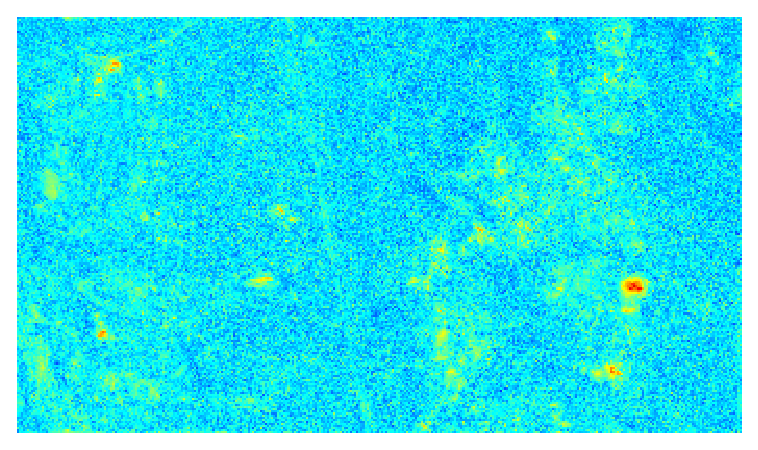
\includegraphics[width=9cm]{./fig/fig_04Expt/64_TGRS_EXPT04_FUMI_REALIMG_MVES_WAY/cuprite1997_200x348/MO16/200x348/DS4/RMSE_MAP_FW}}                 ;
            \node             at (nLeftCenter) [xshift= 4.7cm,yshift=-8.4cm] (nRMSEHYBRID) {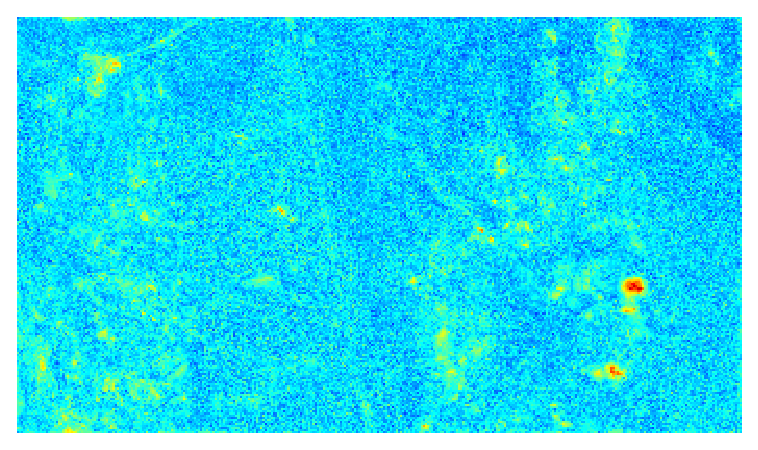
\includegraphics[width=9cm]{./fig/fig_04Expt/64_TGRS_EXPT04_FUMI_REALIMG_MVES_WAY/cuprite1997_200x348/MO16/200x348/DS4/RMSE_MAP_HYBRID}}             ;
            \node[text=white] at (nRMSEFUMI)    [xshift=-3.4cm,yshift= 1.8cm] {\huge FUMI}   ;
            \node[text=white] at (nRMSEPG)      [xshift=-3.7cm,yshift= 1.8cm] {\huge PG}     ;
            \node[text=white] at (nRMSEFISTA)   [xshift=-3.2cm,yshift= 1.8cm] {\huge FISTA}  ;
            \node[text=white] at (nRMSEGP)      [xshift=-3.7cm,yshift= 1.8cm] {\huge GP}     ;
            \node[text=white] at (nRMSEFW)      [xshift=-3.7cm,yshift= 1.8cm] {\huge FW}     ;
            \node[text=white] at (nRMSEHYBRID)  [xshift=-2.8cm,yshift= 1.8cm] {\huge HYBRID} ;
            \node             at (nLeftCenter) [xshift=   0cm,yshift=- 12cm] {\Large (b) RMSE maps} ;
            \node             at (nLeftCenter) [xshift=10.5cm,yshift=-2.5cm] {\includegraphics[width=2.0cm]{./fig/fig_04Expt/64_TGRS_EXPT04_FUMI_REALIMG_MVES_WAY/cuprite1997_200x348/MO16/200x348/DS4/results_cuprite_RMSE_vs_px_colorbar}} ;
        \end{tikzpicture}
    }
	\caption{The RMSE of a trial of semi-real Cuprite dataset simulation. Model
             order $N = 16$; pixel number $L = 200 \times 348$; SNR = $40$dB.}
    \label{fig:results_wfFUMI_cuprite_RMSE}
\end{figure}

\newpage
$\;$
\newpage
\subsection{Results on Semi-real Chikusei Dataset}
We apply FUMI and ALGO to the semi-real Chikusei dataset.
Since the image at hand is relatively large, we set $\delta = 10^{-2}$ to
terminate the algorithms earlier
\footnote{FUMI often encounter numerical error when we feed it with big
HS and MS image pair
In order to enable FUMI to perform HSR successfully, we split
the HS and MS image pair into $100$ smaller pieces and feed them to FUMI one
by one.
Nevertheless FUMI is still unapplicable when model order $N$ is large or when
the noise level is high.
We therefore avoid the comparison whenever it is unavailable.}.
\begin{table}[h]
\centering
\resizebox{0.75\linewidth}{!}{
\begin{threeparttable}
\begin{tabular}{|c|c|c|c|c|c|}
\hline
\multicolumn{ 6}{|c|}{$N = 9$} \tabularnewline \hline
SNR (dB)            & Method                 & RMSE(dB)                              & SAM(deg.)                           & PSNR(dB)                             & Time(sec.)\tnote{3}                      \tabularnewline \hline
%----------------------------------------------------------------------------------------------------------------------------------------------------------------------------------------------------------------%
\multirow{5}{*}{40} & FUMI                   &                    {$-22.58\pm 0.03$} &                    {$2.07\pm 0.01$} &                    {$39.61\pm 0.08$} &                    {$2744.03\pm 440.45$} \tabularnewline
                    & ALGO: PG               &                    {$-22.01\pm 0.03$} &                    {$3.42\pm 0$}    &                    {$36.97\pm 0.06$} &                    {$33.62\pm 8.69$}     \tabularnewline
                    & ALGO: FISTA            & \cellcolor{red! 10}{$-25.12\pm 0$}    & \cellcolor{red! 10}{$1.72\pm 0$}    & \cellcolor{red! 10}{$44.5\pm 0.03$}  &                    {$87.23\pm 21.39$}    \tabularnewline
                    & ALGO: FW               &                    {$-21.72\pm 0.18$} &                    {$3.35\pm 0.14$} &                    {$36.8\pm 0.53$}  &                    {$40.22\pm 11.01$}    \tabularnewline
                    & ALGO: Hybrid \tnote{1} &                    {$-23.08\pm 0.05$} &                    {$2.75\pm 0.04$} &                    {$39.58\pm 0.11$} & \cellcolor{red! 10}{$32.5\pm 8.64$}      \tabularnewline \hline \hline
%----------------------------------------------------------------------------------------------------------------------------------------------------------------------------------------------------------------%
\multirow{5}{*}{30} & FUMI                   &                    {$-21.88\pm 2.21$} &                    {$2.35\pm 0.25$} &                    {$37.71\pm 3.81$} &                    {$4025.73\pm 948.96$} \tabularnewline
                    & ALGO: PG               &                    {$-21.49\pm 2.17$} &                    {$3.56\pm 0.36$} &                    {$35.88\pm 3.62$} &                    {$31.31\pm 8.67$}     \tabularnewline
                    & ALGO: FISTA            & \cellcolor{red! 10}{$-23.44\pm 2.37$} & \cellcolor{red! 10}{$2.26\pm 0.23$} & \cellcolor{red! 10}{$39.71\pm 4.01$} &                    {$52.68\pm 14.96$}    \tabularnewline
                    & ALGO: FW               &                    {$-21.06\pm 2.14$} &                    {$3.44\pm 0.37$} &                    {$35.41\pm 3.68$} &                    {$34.64\pm 10.92$}    \tabularnewline
                    & ALGO: Hybrid \tnote{1} &                    {$-22.43\pm 2.27$} &                    {$2.85\pm 0.29$} &                    {$37.92\pm 3.83$} & \cellcolor{red! 10}{$26.93\pm 9.58$}     \tabularnewline \hline \hline
%----------------------------------------------------------------------------------------------------------------------------------------------------------------------------------------------------------------%
\multirow{5}{*}{20} & FUMI\tnote{2}          & $-$                 & $-$                                 & $-$                                  & $-$                                      \tabularnewline
                    & ALGO: PG               &                    {$-20.25\pm 0.07$} &                    {$4.45\pm 0.13$} &                    {$33.12\pm 0.15$} &                    {$20.83\pm 5.95$}     \tabularnewline
                    & ALGO: FISTA            & \cellcolor{red! 10}{$-20.55\pm 0.07$} &                    {$4.09\pm 0.13$} &                    {$33.56\pm 0.14$} & \cellcolor{red! 10}{$13.21\pm 3.64$}     \tabularnewline
                    & ALGO: FW               &                    {$-19.65\pm 0.2$}  &                    {$4.9\pm 0.28$}  &                    {$32.07\pm 0.4$}  &                    {$21.82\pm 6.14$}     \tabularnewline
                    & ALGO: Hybrid \tnote{1} &                    {$-20.53\pm 0.13$} & \cellcolor{red! 10}{$3.92\pm 0.09$} & \cellcolor{red! 10}{$33.66\pm 0.31$} &                    {$14.26\pm 4.06$}     \tabularnewline \hline
%----------------------------------------------------------------------------------------------------------------------------------------------------------------------------------------------------------------%
\multicolumn{ 6}{|c|}{$N =16$} \tabularnewline \hline
SNR (dB)            & Method                 & RMSE(dB)                              & SAM(deg.)                           & PSNR(dB)                             & Time(sec.)                               \tabularnewline \hline
%----------------------------------------------------------------------------------------------------------------------------------------------------------------------------------------------------------------------------------%
\multirow{5}{*}{40} & FUMI\tnote{2}          & $-$                                   & $-$                                 & $-$                                  & $-$                                      \tabularnewline
                    & ALGO: PG               &                    {$-22.16\pm 0.06$} &                    {$3.36\pm 0.05$} &                    {$37.33\pm 0.16$} & \cellcolor{red! 10}{$56.64\pm 18.45$}    \tabularnewline
                    & ALGO: FISTA            & \cellcolor{red! 10}{$-25.45\pm 0.03$} & \cellcolor{red! 10}{$1.57\pm 0.02$} & \cellcolor{red! 10}{$45.18\pm 0.13$} &                    {$134.76\pm 39.89$}   \tabularnewline
                    & ALGO: FW               &                    {$-22.27\pm 0.1$}  &                    {$3.05\pm 0.06$} &                    {$38.08\pm 0.24$} &                    {$73.03\pm 25.05$}    \tabularnewline
                    & ALGO: Hybrid \tnote{1} &                    {$-23.92\pm 0.07$} &                    {$2.32\pm 0.03$} &                    {$41.38\pm 0.19$} &                    {$67.83\pm 23.9$}     \tabularnewline \hline \hline
%----------------------------------------------------------------------------------------------------------------------------------------------------------------------------------------------------------------------------------%
\multirow{5}{*}{30} & FUMI\tnote{2}          & $-$                                   & $-$                                 & $-$                                  & $-$                                      \tabularnewline
                    & ALGO: PG               &                    {$-21.87\pm 0.08$} &                    {$3.52\pm 0.06$} &                    {$36.62\pm 0.19$} &                    {$52.28\pm 17.2$}     \tabularnewline
                    & ALGO: FISTA            & \cellcolor{red! 10}{$-23.82\pm 0.09$} & \cellcolor{red! 10}{$2.19\pm 0.04$} & \cellcolor{red! 10}{$40.43\pm 0.15$} &                    {$74.44\pm 23.97$}    \tabularnewline
                    & ALGO: FW               &                    {$-21.71\pm 0.09$} &                    {$3.36\pm 0.06$} &                    {$36.47\pm 0.21$} &                    {$57.25\pm 19.24$}    \tabularnewline
                    & ALGO: Hybrid \tnote{1} &                    {$-23.01\pm 0.07$} &                    {$2.72\pm 0.04$} &                    {$38.87\pm 0.1$}  & \cellcolor{red! 10}{$45.14\pm 15.01$}    \tabularnewline \hline \hline
%----------------------------------------------------------------------------------------------------------------------------------------------------------------------------------------------------------------------------------%
\multirow{5}{*}{20} & FUMI\tnote{2}          & $-$                                   & $-$                                 & $-$                                  & $-$                                      \tabularnewline
                    & ALGO: PG               &                    {$-20.36\pm 0.06$} &                    {$4.23\pm 0.12$} &                    {$33.38\pm 0.14$} &                    {$33.36\pm 11.33$}    \tabularnewline
                    & ALGO: FISTA            & \cellcolor{red! 10}{$-20.62\pm 0.08$} & \cellcolor{red! 10}{$3.87\pm 0.13$} &                    {$33.79\pm 0.18$} &                    {$23.09\pm 7.91$}     \tabularnewline
                    & ALGO: FW               &                    {$-19.61\pm 0.12$} &                    {$4.88\pm 0.13$} &                    {$32.08\pm 0.24$} &                    {$29.92\pm 10.06$}    \tabularnewline
                    & ALGO: Hybrid \tnote{1} &                    {$-20.67\pm 0.11$} & \cellcolor{red! 10}{$3.87\pm 0.07$} & \cellcolor{red! 10}{$33.94\pm 0.22$} & \cellcolor{red! 10}{$20.27\pm 6.84$}     \tabularnewline \hline
%----------------------------------------------------------------------------------------------------------------------------------------------------------------------------------------------------------------------------------%
\end{tabular}
\begin{tablenotes}
\item[1] Hybrid update on $\bm S$ by FW and on $\bm A$ by FISTA.
\item[2] FUMI is unable to run on Chikusei under the data settings.
\item[3] The runtime of FUMI is the average total sum of computation time
         required by all $100$ subimages.
\end{tablenotes}
\end{threeparttable}
}
\caption{Average HSR performance on Chikusei dataset by FUMI and ALGO
         $L = 1000 \times 1000$. Highlighted results indicate they are the
         best under the setting.}
\label{table:ALGO_vs_FUMI_REAL_CHIKUSEI_MO9_MO16}
\end{table}

We see from Table \ref{table:ALGO_vs_FUMI_REAL_CHIKUSEI_MO9_MO16} that ALGO
is more capable in processing large images such that FUMI cannot handle the
Chikusei image under when $N = 16$ and under low noise level when $N = 9$.
Regarding the runtime required by the algorithms, ALGO using Hybrid BCD is
almost the fastest.
We qualitatively compare their performance using SAM and RMSE in Figure 
\ref{fig:results_wfFUMI_chikusei_SAM} and
\ref{fig:results_wfFUMI_chikusei_RMSE}, respectively, to show that ALGO using
FISTA is very comparable to FUMI regardless of FUMI's subtle issues.

\begin{figure}
    \centering
    \resizebox{0.98\linewidth}{!}{
        \begin{tikzpicture}
            \node             at (0,0)         [xshift=   0cm,yshift=    0cm] (nLeftCenter){$\;$} ;
            \node             at (0,0)         [xshift=   0cm,yshift=   14cm] (nSAMhist)   {\includegraphics[width=1.40\linewidth]{./fig/fig_04Expt/64_TGRS_EXPT04_FUMI_REALIMG_MVES_WAY/chikusei2014_1000x1000/MO16/1000x1000/DS4/results_chikusei_SAM_vs_px}} ;
            \node             at (nSAMhist)    [xshift=   0cm,yshift=- 4.0cm] {\Large (a) SAM histogram} ;
            \node             at (nLeftCenter) [xshift=-4.7cm,yshift=  4.7cm] (nSAMFUMI)   {\includegraphics[width=9cm]{./fig/fig_04Expt/64_TGRS_EXPT04_FUMI_REALIMG_MVES_WAY/chikusei2014_1000x1000/MO16/1000x1000/DS4/SAM_MAP_FUMI}}               ;
            \node             at (nLeftCenter) [xshift=-4.7cm,yshift=- 4.7cm] (nSAMPG)     {\includegraphics[width=9cm]{./fig/fig_04Expt/64_TGRS_EXPT04_FUMI_REALIMG_MVES_WAY/chikusei2014_1000x1000/MO16/1000x1000/DS4/SAM_MAP_PG}}                 ;
            \node             at (nLeftCenter) [xshift=-4.7cm,yshift=-14.0cm](nSAMFISTA)  {\includegraphics[width=9cm]{./fig/fig_04Expt/64_TGRS_EXPT04_FUMI_REALIMG_MVES_WAY/chikusei2014_1000x1000/MO16/1000x1000/DS4/SAM_MAP_FISTA}}              ;
            \node             at (nLeftCenter) [xshift= 4.7cm,yshift=  4.7cm] (nSAMGP)     {\includegraphics[width=9cm]{./fig/fig_04Expt/64_TGRS_EXPT04_FUMI_REALIMG_MVES_WAY/chikusei2014_1000x1000/MO16/1000x1000/DS4/SAM_MAP_GP}}                 ;
            \node             at (nLeftCenter) [xshift= 4.7cm,yshift=- 4.7cm] (nSAMFW)     {\includegraphics[width=9cm]{./fig/fig_04Expt/64_TGRS_EXPT04_FUMI_REALIMG_MVES_WAY/chikusei2014_1000x1000/MO16/1000x1000/DS4/SAM_MAP_FW}}                 ;
            \node             at (nLeftCenter) [xshift= 4.7cm,yshift=-14.0cm](nSAMHYBRID) {\includegraphics[width=9cm]{./fig/fig_04Expt/64_TGRS_EXPT04_FUMI_REALIMG_MVES_WAY/chikusei2014_1000x1000/MO16/1000x1000/DS4/SAM_MAP_HYBRID}}             ;
            \node[text=white] at (nSAMFUMI)    [xshift=-3.4cm,yshift=  3.8cm] {\huge FUMI}   ;
            \node[text=white] at (nSAMPG)      [xshift=-3.7cm,yshift=  3.8cm] {\huge PG}     ;
            \node[text=white] at (nSAMFISTA)   [xshift=-3.2cm,yshift=  3.8cm] {\huge FISTA}  ;
            \node[text=white] at (nSAMGP)      [xshift=-3.7cm,yshift=  3.8cm] {\huge GP}     ;
            \node[text=white] at (nSAMFW)      [xshift=-3.7cm,yshift=  3.8cm] {\huge FW}     ;
            \node[text=white] at (nSAMHYBRID)  [xshift=-2.8cm,yshift=  3.8cm] {\huge HYBRID} ;
            \node             at (nLeftCenter) [xshift=   0cm,yshift=-  19cm] {\Large (b) SAM maps} ;
            \node             at (nLeftCenter) [xshift=10.5cm,yshift=- 2.5cm] {\includegraphics[width=2.0cm]{./fig/fig_04Expt/64_TGRS_EXPT04_FUMI_REALIMG_MVES_WAY/cuprite1997_200x348/MO16/200x348/DS4/results_cuprite_SAM_vs_px_colorbar}} ;
        \end{tikzpicture}
    }
	\caption{The SAM of a trial of semi-real Chikusei dataset simulation.
             Model order $N = 16$; pixel number $L = 1000 \times 1000$; SNR =
             $40$dB.}
    \label{fig:results_wfFUMI_chikusei_SAM}
\end{figure}

\begin{figure}
    \centering
    \resizebox{0.98\linewidth}{!}{
        \begin{tikzpicture}
            \node             at (0,0)         [xshift=   0cm,yshift=    0cm](nLeftCenter){$\;$} ;
            \node             at (0,0)         [xshift=   0cm,yshift=   14cm](nRMSEhist)   {\includegraphics[width=1.40\linewidth]{./fig/fig_04Expt/64_TGRS_EXPT04_FUMI_REALIMG_MVES_WAY/chikusei2014_1000x1000/MO16/1000x1000/DS4/results_chikusei_RMSE_vs_px}} ;
            \node             at (nRMSEhist)   [xshift=   0cm,yshift=- 4.0cm] {\Large (a) RMSE histogram} ;
            \node             at (nLeftCenter) [xshift=-4.7cm,yshift=  4.7cm](nRMSEFUMI)   {\includegraphics[width=9cm]{./fig/fig_04Expt/64_TGRS_EXPT04_FUMI_REALIMG_MVES_WAY/chikusei2014_1000x1000/MO16/1000x1000/DS4/RMSE_MAP_FUMI}}               ;
            \node             at (nLeftCenter) [xshift=-4.7cm,yshift=- 4.7cm](nRMSEPG)     {\includegraphics[width=9cm]{./fig/fig_04Expt/64_TGRS_EXPT04_FUMI_REALIMG_MVES_WAY/chikusei2014_1000x1000/MO16/1000x1000/DS4/RMSE_MAP_PG}}                 ;
            \node             at (nLeftCenter) [xshift=-4.7cm,yshift=-14.0cm](nRMSEFISTA)  {\includegraphics[width=9cm]{./fig/fig_04Expt/64_TGRS_EXPT04_FUMI_REALIMG_MVES_WAY/chikusei2014_1000x1000/MO16/1000x1000/DS4/RMSE_MAP_FISTA}}              ;
            \node             at (nLeftCenter) [xshift= 4.7cm,yshift=  4.7cm](nRMSEGP)     {\includegraphics[width=9cm]{./fig/fig_04Expt/64_TGRS_EXPT04_FUMI_REALIMG_MVES_WAY/chikusei2014_1000x1000/MO16/1000x1000/DS4/RMSE_MAP_GP}}                 ;
            \node             at (nLeftCenter) [xshift= 4.7cm,yshift=- 4.7cm](nRMSEFW)     {\includegraphics[width=9cm]{./fig/fig_04Expt/64_TGRS_EXPT04_FUMI_REALIMG_MVES_WAY/chikusei2014_1000x1000/MO16/1000x1000/DS4/RMSE_MAP_FW}}                 ;
            \node             at (nLeftCenter) [xshift= 4.7cm,yshift=-14.0cm](nRMSEHYBRID) {\includegraphics[width=9cm]{./fig/fig_04Expt/64_TGRS_EXPT04_FUMI_REALIMG_MVES_WAY/chikusei2014_1000x1000/MO16/1000x1000/DS4/RMSE_MAP_HYBRID}}             ;
            \node[text=white] at (nRMSEFUMI)   [xshift=-3.4cm,yshift=  3.8cm] {\huge FUMI}   ;
            \node[text=white] at (nRMSEPG)     [xshift=-3.7cm,yshift=  3.8cm] {\huge PG}     ;
            \node[text=white] at (nRMSEFISTA)  [xshift=-3.2cm,yshift=  3.8cm] {\huge FISTA}  ;
            \node[text=white] at (nRMSEGP)     [xshift=-3.7cm,yshift=  3.8cm] {\huge GP}     ;
            \node[text=white] at (nRMSEFW)     [xshift=-3.7cm,yshift=  3.8cm] {\huge FW}     ;
            \node[text=white] at (nRMSEHYBRID) [xshift=-2.8cm,yshift=  3.8cm] {\huge HYBRID} ;
            \node             at (nLeftCenter) [xshift=   0cm,yshift=-  19cm]{\Large (b) RMSE maps} ;
            \node             at (nLeftCenter) [xshift=10.5cm,yshift=- 2.5cm]{\includegraphics[width=2.0cm]{./fig/fig_04Expt/64_TGRS_EXPT04_FUMI_REALIMG_MVES_WAY/cuprite1997_200x348/MO16/200x348/DS4/results_cuprite_RMSE_vs_px_colorbar}} ;
        \end{tikzpicture}
    }
	\caption{The RMSE of a trial of semi-real Chikusei dataset simulation.
             Model order $N = 16$; pixel number $L = 1000 \times 1000$; SNR =
             $40$dB.}
    \label{fig:results_wfFUMI_chikusei_RMSE}
\end{figure}

\newpage
\section{Experiment 4: Benchmark HSR via ALGO and CNMF}
\subsection{Results on Semi-real Chikusei Dataset}

We apply CNMF and ALGO to the semi-real Chikusei dataset.
In Yokoya's HSR problem formulation, the feasible set of both $\bm S$ and
$\bm A$ are open ($\mathcal S = \R_+^{N \times L}$ and
$\mathcal A = \R_+^{M \times N}$) so that FW is not directly applicable.
Although as discussed in Section \ref{sec:QP_by_FW} that a heuristic approach
can be used to \textit{simulate} the nonnegative orthant by a nonnegative box
of sufficiently large size, the projection onto nonnegative orthant is in fact
inexpensive so that using FW (and therefore Hybrid BCD) would not have further
advantages under the current HSR problem setting.

For CNMF is popularly known to be a very fast algorithm, we compare it with
FISTA.
Again, since the image at hand is relatively large, we set $\delta = 10^{-2}$
to terminate the algorithms earlier.
\begin{table}[h]
\centering
\resizebox{0.85\linewidth}{!}{
\begin{threeparttable}
\begin{tabular}{|c|c|c|c|c|c|}
\hline
\multicolumn{ 6}{|c|}{$N = 16$} \tabularnewline \hline
SNR (dB)            & Method           & RMSE(dB)                               & SAM(deg.)                             & PSNR(dB)                               & Time(sec.)                               \tabularnewline \hline
%-----------------------------------------------------------------------------------------------------------------------------------------------------------------------------------------------------------------------------%
\multirow{2}{*}{40} & CNMF\tnote{1}    &                    {$28.65    ± 0.02$} &                    {$2.18  \pm 0.01$} &                     {$44.7  \pm 0.04$} & \cellcolor{red! 10} {$39.27 \pm 6.53 $}  \tabularnewline
%                   & CNMF(10it)       &                    {$28.34    ± 0.02$} &                    {$2.28  \pm 0.01$} &                     {$44.28 \pm 0.04$} &                     {$24.2  \pm 3.47 $}  \tabularnewline
                    & ALGO: FISTA      & \cellcolor{red! 10}{$32.18    ± 0.06$} & \cellcolor{red! 10}{$1.61  \pm 0.02$} & \cellcolor{red! 10} {$45.32 \pm 0.11$} &                     {$75.03 \pm 9.76 $}  \tabularnewline \hline \hline
%-----------------------------------------------------------------------------------------------------------------------------------------------------------------------------------------------------------------------------%
\multirow{2}{*}{30} & CNMF\tnote{1}    &                    {$26.59    ± 0.05$} &                    {$2.74  \pm 0.01$} &                     {$39.73 \pm 0.04$} & \cellcolor{red! 10} {$37.6  \pm 7.36 $}  \tabularnewline
%                   & CNMF(10it)       &                    {$26.99    ± 0.01$} &                    {$2.63  \pm 0.01$} &                     {$40.07 \pm 0.02$} &                     {$20.57 \pm 3.54 $}  \tabularnewline
                    & ALGO: FISTA      & \cellcolor{red! 10}{$28.35    ± 1.03$} & \cellcolor{red! 10}{$2.37  \pm 0.31$} & \cellcolor{red! 10} {$40.16 \pm  1  $} &                     {$41.35 \pm 12.92$}  \tabularnewline \hline \hline
%-----------------------------------------------------------------------------------------------------------------------------------------------------------------------------------------------------------------------------%
\multirow{2}{*}{20} & CNMF\tnote{1}    &                    {$21.29    ± 0.1 $} &                    {$4.58  \pm 0.05$} &                     {$32.89 \pm 0.07$} &                     {$33.4  \pm 8.58 $}  \tabularnewline
%                   & CNMF(10it)       &                    {$22.12    ± 0.05$} &                    {$4.02  \pm 0.04$} &                     {$33.66 \pm 0.07$} &                     {$12.11 \pm 2.11 $}  \tabularnewline
                    & ALGO: FISTA      & \cellcolor{red! 10}{$22.44    ± 0.04$} & \cellcolor{red! 10}{$3.73  \pm 0.04$} & \cellcolor{red! 10} {$33.98 \pm 0.06$} & \cellcolor{red! 10} {$11.41 \pm 2.03 $}  \tabularnewline \hline
%-----------------------------------------------------------------------------------------------------------------------------------------------------------------------------------------------------------------------------%
\end{tabular}
\begin{tablenotes}
\item[1] CNMF subproblem iteration number is set to $100$.
\end{tablenotes}
\end{threeparttable}
}
\caption{Average HSR performance on Chikusei dataset by CNMF and ALGO
         $L = 1000 \times 1000$. Highlighted results indicate they are the
         best under the setting.}
\label{table:ALGO_vs_CNMF_REAL_CHIKUSEI_MO9_MO16}
\end{table}

We see from Table \ref{table:ALGO_vs_CNMF_REAL_CHIKUSEI_MO9_MO16} that the HSR
quality by ALGO is similar to that by CNMF in terms of SAM and PSNR and has
obvious improvement in terms of RMSE.
Although ALGO is generally slower than CNMF, we remark that the CNMF algorithm
is not directly solving problem \eqref{eq:HSR_problem_CH3} because it does not
jointly optimize the desired variables with the consideration of the HS and MS
recovery altogether, as shown in the update scheme
\eqref{eq:CNMF_update_A_subproblem} and \eqref{eq:CNMF_update_S_subproblem}.

In Figure \ref{fig:results_wfCNMF_chikusei_SAM} and
\ref{fig:results_wfCNMF_chikusei_RMSE}, we show the SAM and RMSE map of the
recovered Chikusei image.
The performance of ALGO using FISTA is shown to be better than that of CNMF.

\begin{figure}
    \centering
    \resizebox{0.80\linewidth}{!}{
        \begin{tikzpicture}
            \node             at (0,0)         [xshift=   0cm,yshift=    0cm] (nLeftCenter){$\;$} ;
            \node             at (0,0)         [xshift=   0cm,yshift=   14cm] (nSAMhist)   {\includegraphics[width=1.40\linewidth]{./fig/fig_04Expt/67_TGRS_EXPT07_CNMF_REALIMG_MVES_WAY/chikusei2014_1000x1000/MO16/1000x1000/DS4/results_chikusei_SAM_vs_px}} ;
            \node             at (nSAMhist)    [xshift=   0cm,yshift=- 4.0cm] {\Large (a) SAM histogram} ;
            \node             at (nLeftCenter) [xshift=-4.7cm,yshift=  4.7cm] (nSAMCNMF)   {\includegraphics[width=9cm]{./fig/fig_04Expt/67_TGRS_EXPT07_CNMF_REALIMG_MVES_WAY/chikusei2014_1000x1000/MO16/1000x1000/DS4/SAM_MAP_CNMF}}               ;
            \node             at (nLeftCenter) [xshift= 4.7cm,yshift=  4.7cm] (nSAMFISTA)  {\includegraphics[width=9cm]{./fig/fig_04Expt/67_TGRS_EXPT07_CNMF_REALIMG_MVES_WAY/chikusei2014_1000x1000/MO16/1000x1000/DS4/SAM_MAP_FISTA}}              ;
            \node[text=white] at (nSAMCNMF)    [xshift=-3.4cm,yshift=  3.8cm] {\huge CNMF}   ;
            \node[text=white] at (nSAMFISTA)   [xshift=-3.2cm,yshift=  3.8cm] {\huge FISTA}  ;
            \node             at (nLeftCenter) [xshift=   0cm,yshift=-   1cm] {\Large (b) SAM maps} ;
            \node             at (nLeftCenter) [xshift=10.5cm,yshift=    5cm] {\includegraphics[width=1.5cm]{./fig/fig_04Expt/64_TGRS_EXPT04_FUMI_REALIMG_MVES_WAY/cuprite1997_200x348/MO16/200x348/DS4/results_cuprite_SAM_vs_px_colorbar}} ;
        \end{tikzpicture}
    }
	\caption{The SAM of a trial of semi-real Chikusei dataset simulation.
             Model order $N = 16$; pixel number $L = 1000 \times 1000$.}
    \label{fig:results_wfCNMF_chikusei_SAM}
\end{figure}
\begin{figure}
    \centering
    \resizebox{0.80\linewidth}{!}{
        \begin{tikzpicture}
            \node             at (0,0)         [xshift=   0cm,yshift=    0cm] (nLeftCenter){$\;$} ;
            \node             at (0,0)         [xshift=   0cm,yshift=   14cm] (nRMSEhist)   {\includegraphics[width=1.40\linewidth]{./fig/fig_04Expt/67_TGRS_EXPT07_CNMF_REALIMG_MVES_WAY/chikusei2014_1000x1000/MO16/1000x1000/DS4/results_chikusei_RMSE_vs_px}} ;
            \node             at (nRMSEhist)    [xshift=   0cm,yshift=- 4.0cm] {\Large (a) RMSE histogram} ;
            \node             at (nLeftCenter) [xshift=-4.7cm,yshift=  4.7cm] (nRMSECNMF)   {\includegraphics[width=9cm]{./fig/fig_04Expt/67_TGRS_EXPT07_CNMF_REALIMG_MVES_WAY/chikusei2014_1000x1000/MO16/1000x1000/DS4/RMSE_MAP_CNMF}}               ;
            \node             at (nLeftCenter) [xshift= 4.7cm,yshift=  4.7cm] (nRMSEFISTA)  {\includegraphics[width=9cm]{./fig/fig_04Expt/67_TGRS_EXPT07_CNMF_REALIMG_MVES_WAY/chikusei2014_1000x1000/MO16/1000x1000/DS4/RMSE_MAP_FISTA}}              ;
            \node[text=white] at (nRMSECNMF)    [xshift=-3.4cm,yshift=  3.8cm] {\huge CNMF}   ;
            \node[text=white] at (nRMSEFISTA)   [xshift=-3.2cm,yshift=  3.8cm] {\huge FISTA}  ;
            \node             at (nLeftCenter) [xshift=   0cm,yshift=-   1cm] {\Large (b) RMSE maps} ;
            \node             at (nLeftCenter) [xshift=10.5cm,yshift=    5cm] {\includegraphics[width=1.5cm]{./fig/fig_04Expt/64_TGRS_EXPT04_FUMI_REALIMG_MVES_WAY/cuprite1997_200x348/MO16/200x348/DS4/results_cuprite_RMSE_vs_px_colorbar}} ;
        \end{tikzpicture}
    }
	\caption{The RMSE of a trial of semi-real Chikusei dataset simulation.
             Model order $N = 16$; pixel number $L = 1000 \times 1000$.}
    \label{fig:results_wfCNMF_chikusei_RMSE}
\end{figure}
  % The simulations
\chapter{Conclusion and Discussion}
With the increasing demand for faster algorithms in the big data era, massive
data processing technique gains more attraction in the field of computation,
signal processing and data science.
This thesis reviewed a general framework of alternating optimization (AO) on
solving the hyperspectral super-resolution (HSR) problem, which is a kind of
low-rank matrix factorization (MF) problem and is practically attractive in
remote sensing.
Specifically we explored the use of Block Coordinate Descent (BCD) to tackle
the nonconvex HSR problem in two aspects.
The first aspect is the use of Exact BCD and Inexact BCD (whom we proposed as
ALternating Gradient-based Optimization "ALGO") to solve the HSR problem.
Results showed that HSR via ALGO is more competitive than HSR via Exact BCD in
terms of both recovery accuracy and algorithm efficiency, which encouraged us
to focus on Inexact BCD in the remaining of the thesis.
The second aspect is the use of various inexact gradient update rules in
solving each subblock problems in the BCD as a practical and intuitive way to
reduce complexity.
Results showed that proximal type gradient methods are generally better.
Proximal Gradient Method (PG) and Fast Proximal Gradient Method (FISTA) of
this type were shown to be more competitive in terms of recovery accuracy.
Frank Wolfe Method (FW) is also competitive in terms of algorithm efficiency
when the image size and model order are large.

We also compared ALGO with two state-of-the-art HSR algorithms, namely FUMI
and CNMF.
ALGO whom we implemented as a 1-step gradient update in solving each subblock
problem generally possesses comparable recovery performance as FUMI and CNMF
have.
Regarding the computation time, ALGO also demonstrated to be significantly
faster than FUMI even when the data size is very large.

As a future direction, ALGO has great potential in other remote sensing and
machine learning applications as long as we can formulate their problems in a
block-separable manner.
From a practical point of view, ALGO can be applied to existing MF type
problems whose first order information is easily computable.
The advantage of ALGO in terms of computation efficiency can be revealed when
the data size at hand grows to a very large scale and when higher order
methods become impractical.
   % The conclusion

%% ----------------------------------------------------------------
% Now begin the Appendices, including them as separate files

\addtocontents{toc}{\vspace{2em}} % Add a gap in the Contents, for aesthetics

\appendix                         % Cue to tell LaTeX that the following
                                  % 'chapters' are Appendices

\chapter{MATLAB Code of ALGO for Solving Wei et al.'s HSR Problem}

\section{ALGO using GP}
\lstinputlisting[language=Matlab,firstline=23,lastline=89]
                {./code/HSR_MFbA_GP.m}
\newpage
\section{ALGO using BBGP}
\lstinputlisting[language=Matlab,firstline=23,lastline=99]
                {./code/HSR_MFbA_BBGP.m}
\newpage
\section{ALGO using PG}
\lstinputlisting[language=Matlab,firstline=25,lastline=70]
                {./code/HSR_MFbA_PG.m}
\newpage
\section{ALGO using FISTA}
\lstinputlisting[language=Matlab,firstline=25,lastline=82]
                {./code/HSR_MFbA_FISTA.m}
\newpage
\section{ALGO using FW}
\lstinputlisting[language=Matlab,firstline=23,lastline=94]
                {./code/HSR_MFbA_FW.m}
\newpage
\section{ALGO using Hybrid BCD}
\lstinputlisting[language=Matlab,firstline=30,lastline=130]
                {./code/HSR_MFbA_HYBRID.m}
	  % Appendix Title

\chapter{Full Synthetic Simulations Results}
In this section we present the full set of numerical results on synthetic
simulations.
The synthetic simulation settings are detailed in Section \ref{sec:expt_details}.
In the numerical results we take two more quantitative measure than we took in
Chapter 4.
The additional performance measure are normalized mean-squared-error (NMSE) of
the recovered endmember and abundance matrix, which measure their unmixing
error, and reconstruction SNR (RSNR) of the recovered SR image, which measures
the super-resolution error.

The NMSE of estimated endmember matrix $\hat{\bm A}$ and $\hat{\bm S}$ are
defined as
\begin{equation}
    \text{NMSE}(\bm A,\hat{\bm A})
    =
    10 \log_{10} \left(
    \frac{ \Vert \bm A - \hat{\bm A} \Vert\Fr^2 } {\Vert \bm A \Vert\Fr^2}
    \right)
\end{equation}
\begin{equation}
    \text{NMSE}(\bm S,\hat{\bm S})
    =
    10 \log_{10} \left(
    \frac{ \Vert \bm S - \hat{\bm S} \Vert\Fr^2 } {\Vert \bm S \Vert\Fr^2}
    \right),
\end{equation}
respectively.

The RSNR of recovered SR image $\hat{\bm Y}$ is defined as
\begin{equation}
    \text{RSNR}(\bm Y,\hat{\bm Y}) = 10 \log_{10}
    \left( \frac{\Vert\bm Y\Vert\Fr^2} {\Vert\bm Y-\hat{\bm Y}\Vert\Fr^2} \right).
\end{equation}

\section{Performance of ALGO Against the Exactness in solving Subproblems}
We group the results of ALGO into individual tables according to the FOGM that
ALGO uses.
The objective here is to see how the exactness of solving the subproblems
affects ALGO in terms of unmixing and super-resolution quality in the HSR
problem.

In the tables, $J$ refers to the inner iteration number when ALGO solves the
subproblems.
In the context of Hybrid BCD, the notation "$J\sim\mathcal U(a,b)$" reads "$J$
is an integer between $a$ and $b$ following a discrete uniform distribution".
The results by ALGO-GP, ALGO-BBGP, ALGO-PG, ALGO-FISTA, ALGO-FW,
ALGO-Hybrid(S: FW A: PG) and ALGO-Hybrid(S: FW A: PG) are shown from Table
\ref{table:results_full_GP_MO9} to \ref{table:results_full_HYBRID_FW_FISTA_MO9}
where model order $N = 9$.
When $N = 16$, the results are shown from Table \ref{table:results_full_GP_MO16}
to \ref{table:results_full_HYBRID_FW_FISTA_MO16}.

Basically the performance of non-Hybrid type ALGO algorithms are similar to
each other under inexact BCD settings, \ie when $J\in\{1,5,10\}$.
Comparing with exact BCD setting where we take $J=100$, the HU and HSR are
shown to have worse quality.
ALGO-FISTA's performance in Table \ref{table:results_full_FISTA_MO9} and
\ref{table:results_full_FISTA_MO16} (where $N$ is $9$ and $16$, respectively)
can even show a significant difference between the use of exact and inexact BCD.

\begin{table}[h]
\centering
\begin{adjustbox}{max width=\textwidth}
\begin{tabular}{|c|l|c|c|c|c|}
\hline
SNR (dB)            & \multicolumn{1}{c|}{Method}& NMSE-en(dB)         & MSE-en(dB)          & NMSE-ab(dB)         & MSE-ab(dB)          \tabularnewline \hline
%-------------------------------------------------------------------------------------------------------------------------------------------------------------%
\multirow{4}{*}{40} & ALGO-GP ($J=1$)            & $-6.4     \pm 1.76$ & $-8.13    \pm 1.16$ & $-3.81    \pm 0.85$ & $-3.66    \pm 0.86$ \tabularnewline
                    & ALGO-GP ($J=5$)            & $-6.54    \pm 1.83$ & $-8.11    \pm 1.19$ & $-3.84    \pm 0.94$ & $-3.72    \pm 0.95$ \tabularnewline
                    & ALGO-GP ($J=10$)           & $-6.37    \pm 1.8$  & $-8.13    \pm 1.17$ & $-3.85    \pm 0.9$  & $-3.75    \pm 0.91$ \tabularnewline
                    & ALGO-GP ($J=100$)          & $-5.85    \pm 1.57$ & $-7.46    \pm 1.1$  & $-2.75    \pm 0.9$  & $-3.4     \pm 0.85$ \tabularnewline \hline
%-------------------------------------------------------------------------------------------------------------------------------------------------------------%
\multirow{4}{*}{30} & ALGO-GP ($J=1$)            & $-6.27    \pm 1.59$ & $-8.12    \pm 1.11$ & $-3.25    \pm 0.65$ & $-3.2     \pm 0.64$ \tabularnewline
                    & ALGO-GP ($J=5$)            & $-6.31    \pm 1.63$ & $-8.09    \pm 1.17$ & $-3.33    \pm 0.68$ & $-3.27    \pm 0.66$ \tabularnewline
                    & ALGO-GP ($J=10$)           & $-6.23    \pm 1.65$ & $-7.92    \pm 1.18$ & $-3.25    \pm 0.68$ & $-3.23    \pm 0.66$ \tabularnewline
                    & ALGO-GP ($J=100$)          & $-5.67    \pm 1.38$ & $-7.2     \pm 1.02$ & $-2.44    \pm 0.76$ & $-3.09    \pm 0.67$ \tabularnewline \hline
%-------------------------------------------------------------------------------------------------------------------------------------------------------------%
\multirow{4}{*}{20} & ALGO-GP ($J=1$)            & $-5.65    \pm 1.3$  & $-6.75    \pm 0.84$ & $-2.95    \pm 0.48$ & $-2.73    \pm 0.46$ \tabularnewline
                    & ALGO-GP ($J=5$)            & $-5.61    \pm 1.32$ & $-6.54    \pm 0.83$ & $-2.86    \pm 0.48$ & $-2.69    \pm 0.46$ \tabularnewline
                    & ALGO-GP ($J=10$)           & $-5.17    \pm 1.28$ & $-6.24    \pm 0.75$ & $-2.81    \pm 0.47$ & $-2.69    \pm 0.44$ \tabularnewline
                    & ALGO-GP ($J=100$)          & $-3.96    \pm 1.02$ & $-5.1     \pm 0.62$ & $-1.98    \pm 0.55$ & $-2.4     \pm 0.43$ \tabularnewline \hline
%-------------------------------------------------------------------------------------------------------------------------------------------------------------%
\multirow{4}{*}{10} & ALGO-GP ($J=1$)            & $-2.23    \pm 0.79$ & $-3.36    \pm 0.42$ & $-1.28    \pm 0.36$ & $-1.43    \pm 0.29$ \tabularnewline
                    & ALGO-GP ($J=5$)            & $-1.65    \pm 0.71$ & $-2.81    \pm 0.34$ & $-1.28    \pm 0.31$ & $-1.45    \pm 0.27$ \tabularnewline
                    & ALGO-GP ($J=10$)           & $-1.07    \pm 0.68$ & $-2.38    \pm 0.33$ & $-1.22    \pm 0.31$ & $-1.39    \pm 0.26$ \tabularnewline
                    & ALGO-GP ($J=100$)          & $-0.13    \pm 0.63$ & $-1.98    \pm 0.31$ & $-1       \pm 0.27$ & $-1.3     \pm 0.24$ \tabularnewline \hline
%-------------------------------------------------------------------------------------------------------------------------------------------------------------%
\multicolumn{ 6}{ c }{} \tabularnewline
\multicolumn{ 6}{ c }{} \tabularnewline
\multicolumn{ 6}{ c }{} \tabularnewline
\hline
SNR (dB)            & \multicolumn{1}{c|}{Method}& RSNR(dB)            & RMSE(dB)            & SAM(deg.)           & PSNR(dB)            \tabularnewline \hline
%-------------------------------------------------------------------------------------------------------------------------------------------------------------%
\multirow{4}{*}{40} & ALGO-GP ($J=1$)            & $19.34    \pm 1.42$ & $-15.32   \pm 0.65$ & $4.55     \pm 0.69$ & $29.21    \pm 0.92$ \tabularnewline
                    & ALGO-GP ($J=5$)            & $19.36    \pm 1.43$ & $-15.33   \pm 0.67$ & $4.54     \pm 0.7$  & $29.37    \pm 0.98$ \tabularnewline
                    & ALGO-GP ($J=10$)           & $19.49    \pm 1.43$ & $-15.39   \pm 0.64$ & $4.49     \pm 0.71$ & $29.47    \pm 1.05$ \tabularnewline
                    & ALGO-GP ($J=100$)          & $19.24    \pm 1.72$ & $-15.27   \pm 0.89$ & $4.68     \pm 0.76$ & $29.24    \pm 1.34$ \tabularnewline \hline
%-------------------------------------------------------------------------------------------------------------------------------------------------------------%
\multirow{4}{*}{30} & ALGO-GP ($J=1$)            & $19.03    \pm 1.31$ & $-15.17   \pm 0.71$ & $4.9      \pm 0.63$ & $26.93    \pm 0.78$ \tabularnewline
                    & ALGO-GP ($J=5$)            & $18.99    \pm 1.37$ & $-15.15   \pm 0.69$ & $4.92     \pm 0.69$ & $27.02    \pm 0.77$ \tabularnewline
                    & ALGO-GP ($J=10$)           & $18.85    \pm 1.36$ & $-15.08   \pm 0.66$ & $5        \pm 0.71$ & $26.93    \pm 0.78$ \tabularnewline
                    & ALGO-GP ($J=100$)          & $18.77    \pm 1.46$ & $-15.04   \pm 0.76$ & $5.32     \pm 0.71$ & $26.73    \pm 0.98$ \tabularnewline \hline
%-------------------------------------------------------------------------------------------------------------------------------------------------------------%
\multirow{4}{*}{20} & ALGO-GP ($J=1$)            & $17.13    \pm 0.87$ & $-14.21   \pm 0.58$ & $6.69     \pm 0.57$ & $23.07    \pm 0.67$ \tabularnewline
                    & ALGO-GP ($J=5$)            & $17.03    \pm 0.88$ & $-14.16   \pm 0.58$ & $6.82     \pm 0.56$ & $23.03    \pm 0.7$  \tabularnewline
                    & ALGO-GP ($J=10$)           & $16.8     \pm 0.83$ & $-14.05   \pm 0.58$ & $7.12     \pm 0.52$ & $22.83    \pm 0.72$ \tabularnewline
                    & ALGO-GP ($J=100$)          & $16.27    \pm 0.69$ & $-13.78   \pm 0.6$  & $8.17     \pm 0.51$ & $22.21    \pm 0.97$ \tabularnewline \hline
%-------------------------------------------------------------------------------------------------------------------------------------------------------------%
\multirow{4}{*}{10} & ALGO-GP ($J=1$)            & $11.36    \pm 0.33$ & $-11.34   \pm 0.7$  & $14.11    \pm 0.54$ & $16.96    \pm 0.79$ \tabularnewline
                    & ALGO-GP ($J=5$)            & $10.69    \pm 0.26$ & $-11      \pm 0.74$ & $15.44    \pm 0.49$ & $16.27    \pm 0.87$ \tabularnewline
                    & ALGO-GP ($J=10$)           & $10.11    \pm 0.25$ & $-10.72   \pm 0.74$ & $16.61    \pm 0.49$ & $15.68    \pm 0.91$ \tabularnewline
                    & ALGO-GP ($J=100$)          & $9.17     \pm 0.29$ & $-10.24   \pm 0.66$ & $18.6     \pm 0.6$  & $14.72    \pm 0.89$ \tabularnewline \hline
%-------------------------------------------------------------------------------------------------------------------------------------------------------------%
\multicolumn{ 6}{ c }{} \tabularnewline
\multicolumn{ 6}{ c }{} \tabularnewline
\multicolumn{ 6}{ c }{} \tabularnewline
\cline{1-4}
SNR (dB)            & \multicolumn{1}{c|}{Method}& Time(sec)             & Outer Iter.           \tabularnewline \cline{1-4}
%--------------------------------------------------------------------------------------------------------------------------%
\multirow{4}{*}{40} & ALGO-GP ($J=1$)            & $15.82    \pm 4.55$   & $1233.2   \pm 246.73$ \tabularnewline
                    & ALGO-GP ($J=5$)            & $35.67    \pm 11.22$  & $673.81   \pm 149.42$ \tabularnewline
                    & ALGO-GP ($J=10$)           & $50.87    \pm 16.77$  & $493.34   \pm 128.56$ \tabularnewline
                    & ALGO-GP ($J=100$)          & $322.16   \pm 109.76$ & $298.53   \pm 72.13$  \tabularnewline \cline{1-4}
%--------------------------------------------------------------------------------------------------------------------------%
\multirow{4}{*}{30} & ALGO-GP ($J=1$)            & $7.91     \pm 2.01$   & $558.76   \pm 91.89$  \tabularnewline
                    & ALGO-GP ($J=5$)            & $14.73    \pm 3.74$   & $261.58   \pm 34.84$  \tabularnewline
                    & ALGO-GP ($J=10$)           & $22.58    \pm 5.67$   & $202.9    \pm 26.3$   \tabularnewline
                    & ALGO-GP ($J=100$)          & $133.94   \pm 39.43$  & $111.88   \pm 16.49$  \tabularnewline \cline{1-4}
%--------------------------------------------------------------------------------------------------------------------------%
\multirow{4}{*}{20} & ALGO-GP ($J=1$)            & $2.32     \pm 0.54$   & $165.91   \pm 21.13$  \tabularnewline
                    & ALGO-GP ($J=5$)            & $5.42     \pm 1.29$   & $103.28   \pm 9.86$   \tabularnewline
                    & ALGO-GP ($J=10$)           & $9.32     \pm 2.3$    & $90       \pm 10.86$  \tabularnewline
                    & ALGO-GP ($J=100$)          & $58.3     \pm 17.71$  & $52.73    \pm 6.87$   \tabularnewline \cline{1-4}
%--------------------------------------------------------------------------------------------------------------------------%
\multirow{4}{*}{10} & ALGO-GP ($J=1$)            & $1.76     \pm 0.4$    & $124.84   \pm 11.45$  \tabularnewline
                    & ALGO-GP ($J=5$)            & $3.26     \pm 0.81$   & $62.09    \pm 6.09$   \tabularnewline
                    & ALGO-GP ($J=10$)           & $5.21     \pm 1.47$   & $50.62    \pm 8.73$   \tabularnewline
                    & ALGO-GP ($J=100$)          & $49.51    \pm 15.78$  & $43.49    \pm 7.73$   \tabularnewline \cline{1-4}
%--------------------------------------------------------------------------------------------------------------------------%
\end{tabular}
\end{adjustbox}
\caption{Average HU and HSR performance of ALGO-GP on synthetic data.
         $N = 9$; $L = 100 \times 100$; $1000$ trials.}
\label{table:results_full_GP_MO9}
\end{table}

\newpage

\begin{table}[h]
\centering
\begin{adjustbox}{max width=\textwidth}
\begin{tabular}{|c|l|c|c|c|c|}
\hline
SNR (dB)            & \multicolumn{1}{c|}{Method}  & NMSE-en(dB)         & MSE-en(dB)          & NMSE-ab(dB)         & MSE-ab(dB)          \tabularnewline \hline
%---------------------------------------------------------------------------------------------------------------------------------------------------------------%
\multirow{4}{*}{40} & ALGO-BBGP ($J=1$)            & $-6.4     \pm 1.67$ & $-8.24    \pm 1.12$ & $-3.65    \pm 0.83$ & $-3.62    \pm 0.83$ \tabularnewline
                    & ALGO-BBGP ($J=5$)            & $-6.46    \pm 1.69$ & $-8.2     \pm 1.13$ & $-3.77    \pm 0.83$ & $-3.72    \pm 0.83$ \tabularnewline
                    & ALGO-BBGP ($J=10$)           & $-6.43    \pm 1.7$  & $-8.06    \pm 1.15$ & $-3.75    \pm 0.86$ & $-3.74    \pm 0.88$ \tabularnewline
                    & ALGO-BBGP ($J=100$)          & $-5.92    \pm 1.56$ & $-7.47    \pm 1.1$  & $-2.75    \pm 0.9$  & $-3.43    \pm 0.83$ \tabularnewline \hline
%---------------------------------------------------------------------------------------------------------------------------------------------------------------%
\multirow{4}{*}{30} & ALGO-BBGP ($J=1$)            & $-6.27    \pm 1.59$ & $-8.12    \pm 1.11$ & $-3.25    \pm 0.65$ & $-3.2     \pm 0.64$ \tabularnewline
                    & ALGO-BBGP ($J=5$)            & $-6.31    \pm 1.63$ & $-8.09    \pm 1.17$ & $-3.33    \pm 0.68$ & $-3.27    \pm 0.66$ \tabularnewline
                    & ALGO-BBGP ($J=10$)           & $-6.23    \pm 1.65$ & $-7.92    \pm 1.18$ & $-3.25    \pm 0.68$ & $-3.23    \pm 0.66$ \tabularnewline
                    & ALGO-BBGP ($J=100$)          & $-5.67    \pm 1.38$ & $-7.2     \pm 1.02$ & $-2.44    \pm 0.76$ & $-3.09    \pm 0.67$ \tabularnewline \hline
%---------------------------------------------------------------------------------------------------------------------------------------------------------------%
\multirow{4}{*}{20} & ALGO-BBGP ($J=1$)            & $-5.64    \pm 1.2$  & $-6.88    \pm 0.79$ & $-2.48    \pm 0.47$ & $-2.45    \pm 0.43$ \tabularnewline
                    & ALGO-BBGP ($J=5$)            & $-5.47    \pm 1.24$ & $-6.6     \pm 0.78$ & $-2.6     \pm 0.47$ & $-2.55    \pm 0.43$ \tabularnewline
                    & ALGO-BBGP ($J=10$)           & $-5.3     \pm 1.23$ & $-6.35    \pm 0.79$ & $-2.52    \pm 0.47$ & $-2.5     \pm 0.42$ \tabularnewline
                    & ALGO-BBGP ($J=100$)          & $-4.18    \pm 1.02$ & $-5.26    \pm 0.62$ & $-1.99    \pm 0.54$ & $-2.4     \pm 0.42$ \tabularnewline \hline
%---------------------------------------------------------------------------------------------------------------------------------------------------------------%
\multirow{4}{*}{10} & ALGO-BBGP ($J=1$)            & $-2.27    \pm 0.71$ & $-3.52    \pm 0.37$ & $-1       \pm 0.31$ & $-1.31    \pm 0.25$ \tabularnewline
                    & ALGO-BBGP ($J=5$)            & $-1.45    \pm 0.67$ & $-2.84    \pm 0.31$ & $-1.09    \pm 0.3$  & $-1.37    \pm 0.25$ \tabularnewline
                    & ALGO-BBGP ($J=10$)           & $-1.22    \pm 0.66$ & $-2.58    \pm 0.31$ & $-1.11    \pm 0.29$ & $-1.36    \pm 0.25$ \tabularnewline
                    & ALGO-BBGP ($J=100$)          & $-0.2     \pm 0.63$ & $-2       \pm 0.31$ & $-1       \pm 0.26$ & $-1.3     \pm 0.24$ \tabularnewline \hline
%---------------------------------------------------------------------------------------------------------------------------------------------------------------%
\multicolumn{ 6}{ c }{} \tabularnewline
\multicolumn{ 6}{ c }{} \tabularnewline
\multicolumn{ 6}{ c }{} \tabularnewline
\hline
SNR (dB)            & \multicolumn{1}{c|}{Method}  & RSNR(dB)            & RMSE(dB)            & SAM(deg.)           & PSNR(dB)            \tabularnewline \hline
%---------------------------------------------------------------------------------------------------------------------------------------------------------------%
\multirow{4}{*}{40} & ALGO-BBGP ($J=1$)            & $19.57    \pm 1.41$ & $-15.43   \pm 0.75$ & $4.38     \pm 0.66$ & $29.38    \pm 0.95$ \tabularnewline
                    & ALGO-BBGP ($J=5$)            & $19.48    \pm 1.44$ & $-15.39   \pm 0.75$ & $4.43     \pm 0.69$ & $29.47    \pm 0.97$ \tabularnewline
                    & ALGO-BBGP ($J=10$)           & $19.42    \pm 1.41$ & $-15.36   \pm 0.72$ & $4.46     \pm 0.69$ & $29.43    \pm  1$   \tabularnewline
                    & ALGO-BBGP ($J=100$)          & $19.36    \pm 1.67$ & $-15.33   \pm 0.89$ & $4.66     \pm 0.75$ & $29.32    \pm 1.3$  \tabularnewline \hline
%---------------------------------------------------------------------------------------------------------------------------------------------------------------%
\multirow{4}{*}{30} & ALGO-BBGP ($J=1$)            & $19.03    \pm 1.31$ & $-15.17   \pm 0.71$ & $4.9      \pm 0.63$ & $26.93    \pm 0.78$ \tabularnewline
                    & ALGO-BBGP ($J=5$)            & $18.99    \pm 1.37$ & $-15.15   \pm 0.69$ & $4.92     \pm 0.69$ & $27.02    \pm 0.77$ \tabularnewline
                    & ALGO-BBGP ($J=10$)           & $18.85    \pm 1.36$ & $-15.08   \pm 0.66$ & $5        \pm 0.71$ & $26.93    \pm 0.78$ \tabularnewline
                    & ALGO-BBGP ($J=100$)          & $18.77    \pm 1.46$ & $-15.04   \pm 0.76$ & $5.32     \pm 0.71$ & $26.73    \pm 0.98$ \tabularnewline \hline
%---------------------------------------------------------------------------------------------------------------------------------------------------------------%
\multirow{4}{*}{20} & ALGO-BBGP ($J=1$)            & $16.98    \pm 0.85$ & $-14.13   \pm 0.6$  & $6.79     \pm 0.57$ & $22.93    \pm 0.73$ \tabularnewline
                    & ALGO-BBGP ($J=5$)            & $17       \pm 0.89$ & $-14.15   \pm 0.6$  & $6.87     \pm 0.57$ & $23.01    \pm 0.75$ \tabularnewline
                    & ALGO-BBGP ($J=10$)           & $16.78    \pm 0.86$ & $-14.04   \pm 0.6$  & $7.08     \pm 0.56$ & $22.84    \pm 0.76$ \tabularnewline
                    & ALGO-BBGP ($J=100$)          & $16.38    \pm 0.7$  & $-13.84   \pm 0.59$ & $8.03     \pm 0.5$  & $22.33    \pm 0.96$ \tabularnewline \hline
%---------------------------------------------------------------------------------------------------------------------------------------------------------------%
\multirow{4}{*}{10} & ALGO-BBGP ($J=1$)            & $11.29    \pm 0.33$ & $-11.31   \pm 0.68$ & $14.22    \pm 0.54$ & $16.89    \pm 0.78$ \tabularnewline
                    & ALGO-BBGP ($J=5$)            & $10.55    \pm 0.26$ & $-10.93   \pm 0.73$ & $15.7     \pm 0.48$ & $16.12    \pm 0.88$ \tabularnewline
                    & ALGO-BBGP ($J=10$)           & $10.25    \pm 0.24$ & $-10.79   \pm 0.74$ & $16.32    \pm 0.47$ & $15.82    \pm 0.89$ \tabularnewline
                    & ALGO-BBGP ($J=100$)          & $9.23     \pm 0.28$ & $-10.27   \pm 0.67$ & $18.47    \pm 0.57$ & $14.78    \pm 0.89$ \tabularnewline \hline
%---------------------------------------------------------------------------------------------------------------------------------------------------------------%
\multicolumn{ 6}{ c }{} \tabularnewline
\multicolumn{ 6}{ c }{} \tabularnewline
\multicolumn{ 6}{ c }{} \tabularnewline
\cline{1-4}
SNR (dB)            & \multicolumn{1}{c|}{Method}  & Time(sec)             & Outer Iter.           \tabularnewline \cline{1-4}
%----------------------------------------------------------------------------------------------------------------------------%
\multirow{4}{*}{40} & ALGO-BBGP ($J=1$)            & $18.06    \pm 4.82$   & $1303.63  \pm 238.66$ \tabularnewline
                    & ALGO-BBGP ($J=5$)            & $40       \pm 11.75$  & $697.8    \pm 139.47$ \tabularnewline
                    & ALGO-BBGP ($J=10$)           & $61.17    \pm 19.16$  & $541.8    \pm 123.03$ \tabularnewline
                    & ALGO-BBGP ($J=100$)          & $352.19   \pm 119.94$ & $297.17   \pm 70.9$   \tabularnewline \cline{1-4}
%----------------------------------------------------------------------------------------------------------------------------%
\multirow{4}{*}{30} & ALGO-BBGP ($J=1$)            & $7.91     \pm 2.01$   & $558.76   \pm 91.89$  \tabularnewline
                    & ALGO-BBGP ($J=5$)            & $14.73    \pm 3.74$   & $261.58   \pm 34.84$  \tabularnewline
                    & ALGO-BBGP ($J=10$)           & $22.58    \pm 5.67$   & $202.9    \pm 26.3$   \tabularnewline
                    & ALGO-BBGP ($J=100$)          & $133.94   \pm 39.43$  & $111.88   \pm 16.49$  \tabularnewline \cline{1-4}
%----------------------------------------------------------------------------------------------------------------------------%
\multirow{4}{*}{20} & ALGO-BBGP ($J=1$)            & $3.66     \pm 0.84$   & $245.73   \pm 33.62$  \tabularnewline
                    & ALGO-BBGP ($J=5$)            & $6.52     \pm 1.59$   & $115.68   \pm 13.43$  \tabularnewline
                    & ALGO-BBGP ($J=10$)           & $11.71    \pm 2.69$   & $104.36   \pm 8.82$   \tabularnewline
                    & ALGO-BBGP ($J=100$)          & $69.44    \pm 19.71$  & $57.3     \pm 6.19$   \tabularnewline \cline{1-4}
%----------------------------------------------------------------------------------------------------------------------------%
\multirow{4}{*}{10} & ALGO-BBGP ($J=1$)            & $2.04     \pm 0.49$   & $136.03   \pm 17.53$  \tabularnewline
                    & ALGO-BBGP ($J=5$)            & $4.3      \pm 1.03$   & $75.21    \pm 8.62$   \tabularnewline
                    & ALGO-BBGP ($J=10$)           & $7.81     \pm 1.89$   & $69.14    \pm 8.14$   \tabularnewline
                    & ALGO-BBGP ($J=100$)          & $54.66    \pm 16.97$  & $44.92    \pm 7.51$   \tabularnewline \cline{1-4}
%----------------------------------------------------------------------------------------------------------------------------%
\end{tabular}                                                                                                                                                  
\end{adjustbox}                                                                                                                                                
\caption{Average HU and HSR performance of ALGO-BBGP on synthetic data.                                                                                        
         $N = 9$; $L = 100 \times 100$; $1000$ trials.}                                                                                            
\label{table:results_full_BBGP_MO9}
\end{table}

\newpage

\begin{table}[h]
\centering
\begin{adjustbox}{max width=\textwidth}
\begin{tabular}{|c|l|c|c|c|c|}
\hline
SNR (dB)            & \multicolumn{1}{c|}{Method}& NMSE-en(dB)         & MSE-en(dB)          & NMSE-ab(dB)         & MSE-ab(dB)          \tabularnewline \hline
%-------------------------------------------------------------------------------------------------------------------------------------------------------------%
\multirow{4}{*}{40} & ALGO-PG ($J=1$)            & $-6.4     \pm 1.67$ & $-8.24    \pm 1.12$ & $-3.65    \pm 0.83$ & $-3.62    \pm 0.83$ \tabularnewline
                    & ALGO-PG ($J=5$)            & $-6.46    \pm 1.69$ & $-8.2     \pm 1.13$ & $-3.77    \pm 0.83$ & $-3.72    \pm 0.83$ \tabularnewline
                    & ALGO-PG ($J=10$)           & $-6.43    \pm 1.7$  & $-8.06    \pm 1.15$ & $-3.75    \pm 0.86$ & $-3.74    \pm 0.88$ \tabularnewline
                    & ALGO-PG ($J=100$)          & $-5.92    \pm 1.56$ & $-7.47    \pm 1.1$  & $-2.75    \pm 0.9$  & $-3.43    \pm 0.83$ \tabularnewline \hline
%-------------------------------------------------------------------------------------------------------------------------------------------------------------%
\multirow{4}{*}{30} & ALGO-PG ($J=1$)            & $-6.27    \pm 1.59$ & $-8.12    \pm 1.11$ & $-3.25    \pm 0.65$ & $-3.2     \pm 0.64$ \tabularnewline
                    & ALGO-PG ($J=5$)            & $-6.31    \pm 1.63$ & $-8.09    \pm 1.17$ & $-3.33    \pm 0.68$ & $-3.27    \pm 0.66$ \tabularnewline
                    & ALGO-PG ($J=10$)           & $-6.23    \pm 1.65$ & $-7.92    \pm 1.18$ & $-3.25    \pm 0.68$ & $-3.23    \pm 0.66$ \tabularnewline
                    & ALGO-PG ($J=100$)          & $-5.67    \pm 1.38$ & $-7.2     \pm 1.02$ & $-2.44    \pm 0.76$ & $-3.09    \pm 0.67$ \tabularnewline \hline
%-------------------------------------------------------------------------------------------------------------------------------------------------------------%
\multirow{4}{*}{20} & ALGO-PG ($J=1$)            & $-5.64    \pm 1.2$  & $-6.88    \pm 0.79$ & $-2.48    \pm 0.47$ & $-2.45    \pm 0.43$ \tabularnewline
                    & ALGO-PG ($J=5$)            & $-5.47    \pm 1.24$ & $-6.6     \pm 0.78$ & $-2.6     \pm 0.47$ & $-2.55    \pm 0.43$ \tabularnewline
                    & ALGO-PG ($J=10$)           & $-5.3     \pm 1.23$ & $-6.35    \pm 0.79$ & $-2.52    \pm 0.47$ & $-2.5     \pm 0.42$ \tabularnewline
                    & ALGO-PG ($J=100$)          & $-4.18    \pm 1.02$ & $-5.26    \pm 0.62$ & $-1.99    \pm 0.54$ & $-2.4     \pm 0.42$ \tabularnewline \hline
%-------------------------------------------------------------------------------------------------------------------------------------------------------------%
\multirow{4}{*}{10} & ALGO-PG ($J=1$)            & $-2.27    \pm 0.71$ & $-3.52    \pm 0.37$ & $-1       \pm 0.31$ & $-1.31    \pm 0.25$ \tabularnewline
                    & ALGO-PG ($J=5$)            & $-1.45    \pm 0.67$ & $-2.84    \pm 0.31$ & $-1.09    \pm 0.3$  & $-1.37    \pm 0.25$ \tabularnewline
                    & ALGO-PG ($J=10$)           & $-1.22    \pm 0.66$ & $-2.58    \pm 0.31$ & $-1.11    \pm 0.29$ & $-1.36    \pm 0.25$ \tabularnewline
                    & ALGO-PG ($J=100$)          & $-0.2     \pm 0.63$ & $-2       \pm 0.31$ & $-1       \pm 0.26$ & $-1.3     \pm 0.24$ \tabularnewline \hline
%-------------------------------------------------------------------------------------------------------------------------------------------------------------%
\multicolumn{ 6}{ c }{} \tabularnewline
\multicolumn{ 6}{ c }{} \tabularnewline
\multicolumn{ 6}{ c }{} \tabularnewline
\hline
SNR (dB)            & \multicolumn{1}{c|}{Method}& RSNR(dB)            & RMSE(dB)            & SAM(deg.)           & PSNR(dB)            \tabularnewline \hline
%-------------------------------------------------------------------------------------------------------------------------------------------------------------%
\multirow{4}{*}{40} & ALGO-PG ($J=1$)            & $19.57    \pm 1.41$ & $-15.43   \pm 0.75$ & $4.38     \pm 0.66$ & $29.38    \pm 0.95$ \tabularnewline
                    & ALGO-PG ($J=5$)            & $19.48    \pm 1.44$ & $-15.39   \pm 0.75$ & $4.43     \pm 0.69$ & $29.47    \pm 0.97$ \tabularnewline
                    & ALGO-PG ($J=10$)           & $19.42    \pm 1.41$ & $-15.36   \pm 0.72$ & $4.46     \pm 0.69$ & $29.43    \pm  1$   \tabularnewline
                    & ALGO-PG ($J=100$)          & $19.36    \pm 1.67$ & $-15.33   \pm 0.89$ & $4.66     \pm 0.75$ & $29.32    \pm 1.3$  \tabularnewline \hline
%-------------------------------------------------------------------------------------------------------------------------------------------------------------%
\multirow{4}{*}{30} & ALGO-PG ($J=1$)            & $19.03    \pm 1.31$ & $-15.17   \pm 0.71$ & $4.9      \pm 0.63$ & $26.93    \pm 0.78$ \tabularnewline
                    & ALGO-PG ($J=5$)            & $18.99    \pm 1.37$ & $-15.15   \pm 0.69$ & $4.92     \pm 0.69$ & $27.02    \pm 0.77$ \tabularnewline
                    & ALGO-PG ($J=10$)           & $18.85    \pm 1.36$ & $-15.08   \pm 0.66$ & $5        \pm 0.71$ & $26.93    \pm 0.78$ \tabularnewline
                    & ALGO-PG ($J=100$)          & $18.77    \pm 1.46$ & $-15.04   \pm 0.76$ & $5.32     \pm 0.71$ & $26.73    \pm 0.98$ \tabularnewline \hline
%-------------------------------------------------------------------------------------------------------------------------------------------------------------%
\multirow{4}{*}{20} & ALGO-PG ($J=1$)            & $16.98    \pm 0.85$ & $-14.13   \pm 0.6$  & $6.79     \pm 0.57$ & $22.93    \pm 0.73$ \tabularnewline
                    & ALGO-PG ($J=5$)            & $17       \pm 0.89$ & $-14.15   \pm 0.6$  & $6.87     \pm 0.57$ & $23.01    \pm 0.75$ \tabularnewline
                    & ALGO-PG ($J=10$)           & $16.78    \pm 0.86$ & $-14.04   \pm 0.6$  & $7.08     \pm 0.56$ & $22.84    \pm 0.76$ \tabularnewline
                    & ALGO-PG ($J=100$)          & $16.38    \pm 0.7$  & $-13.84   \pm 0.59$ & $8.03     \pm 0.5$  & $22.33    \pm 0.96$ \tabularnewline \hline
%-------------------------------------------------------------------------------------------------------------------------------------------------------------%
\multirow{4}{*}{10} & ALGO-PG ($J=1$)            & $11.29    \pm 0.33$ & $-11.31   \pm 0.68$ & $14.22    \pm 0.54$ & $16.89    \pm 0.78$ \tabularnewline
                    & ALGO-PG ($J=5$)            & $10.55    \pm 0.26$ & $-10.93   \pm 0.73$ & $15.7     \pm 0.48$ & $16.12    \pm 0.88$ \tabularnewline
                    & ALGO-PG ($J=10$)           & $10.25    \pm 0.24$ & $-10.79   \pm 0.74$ & $16.32    \pm 0.47$ & $15.82    \pm 0.89$ \tabularnewline
                    & ALGO-PG ($J=100$)          & $9.23     \pm 0.28$ & $-10.27   \pm 0.67$ & $18.47    \pm 0.57$ & $14.78    \pm 0.89$ \tabularnewline \hline
%-------------------------------------------------------------------------------------------------------------------------------------------------------------%
\multicolumn{ 6}{ c }{} \tabularnewline
\multicolumn{ 6}{ c }{} \tabularnewline
\multicolumn{ 6}{ c }{} \tabularnewline
\cline{1-4}
SNR (dB)            & \multicolumn{1}{c|}{Method}& Time(sec)             & Outer Iter.           \tabularnewline \cline{1-4}
%--------------------------------------------------------------------------------------------------------------------------%
\multirow{4}{*}{40} & ALGO-PG ($J=1$)            & $18.06    \pm 4.82$   & $1303.63  \pm 238.66$ \tabularnewline
                    & ALGO-PG ($J=5$)            & $40       \pm 11.75$  & $697.8    \pm 139.47$ \tabularnewline
                    & ALGO-PG ($J=10$)           & $61.17    \pm 19.16$  & $541.8    \pm 123.03$ \tabularnewline
                    & ALGO-PG ($J=100$)          & $352.19   \pm 119.94$ & $297.17   \pm 70.9$   \tabularnewline \cline{1-4}
%--------------------------------------------------------------------------------------------------------------------------%
\multirow{4}{*}{30} & ALGO-PG ($J=1$)            & $7.91     \pm 2.01$   & $558.76   \pm 91.89$  \tabularnewline
                    & ALGO-PG ($J=5$)            & $14.73    \pm 3.74$   & $261.58   \pm 34.84$  \tabularnewline
                    & ALGO-PG ($J=10$)           & $22.58    \pm 5.67$   & $202.9    \pm 26.3$   \tabularnewline
                    & ALGO-PG ($J=100$)          & $133.94   \pm 39.43$  & $111.88   \pm 16.49$  \tabularnewline \cline{1-4}
%--------------------------------------------------------------------------------------------------------------------------%
\multirow{4}{*}{20} & ALGO-PG ($J=1$)            & $3.66     \pm 0.84$   & $245.73   \pm 33.62$  \tabularnewline
                    & ALGO-PG ($J=5$)            & $6.52     \pm 1.59$   & $115.68   \pm 13.43$  \tabularnewline
                    & ALGO-PG ($J=10$)           & $11.71    \pm 2.69$   & $104.36   \pm 8.82$   \tabularnewline
                    & ALGO-PG ($J=100$)          & $69.44    \pm 19.71$  & $57.3     \pm 6.19$   \tabularnewline \cline{1-4}
%--------------------------------------------------------------------------------------------------------------------------%
\multirow{4}{*}{10} & ALGO-PG ($J=1$)            & $2.04     \pm 0.49$   & $136.03   \pm 17.53$  \tabularnewline
                    & ALGO-PG ($J=5$)            & $4.3      \pm 1.03$   & $75.21    \pm 8.62$   \tabularnewline
                    & ALGO-PG ($J=10$)           & $7.81     \pm 1.89$   & $69.14    \pm 8.14$   \tabularnewline
                    & ALGO-PG ($J=100$)          & $54.66    \pm 16.97$  & $44.92    \pm 7.51$   \tabularnewline \cline{1-4}
%--------------------------------------------------------------------------------------------------------------------------%
\end{tabular}                                                                                                                                                  
\end{adjustbox}                                                                                                                                                
\caption{Average HU and HSR performance of ALGO-PG on synthetic data.                                                                                        
         $N = 9$; $L = 100 \times 100$; $1000$ trials.}                                                                                            
\label{table:results_full_PG_MO9}
\end{table}

\newpage

\begin{table}[h]
\centering
\begin{adjustbox}{max width=\textwidth}
\begin{tabular}{|c|l|c|c|c|c|}
\hline
SNR (dB)            & \multicolumn{1}{c|}{Method}   & NMSE-en(dB)         & MSE-en(dB)          & NMSE-ab(dB)         & MSE-ab(dB)          \tabularnewline \hline
%----------------------------------------------------------------------------------------------------------------------------------------------------------------%
\multirow{4}{*}{40} & ALGO-FISTA ($J=1$)            & $-6.89    \pm 1.99$ & $-7.99    \pm 1.17$ & $-4.27    \pm 0.82$ & $-4.08    \pm 0.84$ \tabularnewline
                    & ALGO-FISTA ($J=5$)            & $-6.94    \pm 1.99$ & $-7.95    \pm 1.19$ & $-4.35    \pm 0.85$ & $-4.17    \pm 0.87$ \tabularnewline
                    & ALGO-FISTA ($J=10$)           & $-6.8     \pm 1.95$ & $-7.96    \pm 1.21$ & $-4.29    \pm 0.87$ & $-4.16    \pm 0.89$ \tabularnewline
                    & ALGO-FISTA ($J=100$)          & $-5.72    \pm 1.75$ & $-7.4     \pm 1.18$ & $-2.76    \pm 0.85$ & $-3.42    \pm 0.84$ \tabularnewline \hline
%----------------------------------------------------------------------------------------------------------------------------------------------------------------%
\multirow{4}{*}{30} & ALGO-FISTA ($J=1$)            & $-6.42    \pm 1.71$ & $-7.6     \pm 1.08$ & $-3.77    \pm 0.62$ & $-3.55    \pm 0.61$ \tabularnewline
                    & ALGO-FISTA ($J=5$)            & $-6.21    \pm 1.71$ & $-7.19    \pm 1.02$ & $-3.86    \pm 0.63$ & $-3.65    \pm 0.62$ \tabularnewline
                    & ALGO-FISTA ($J=10$)           & $-6.06    \pm 1.66$ & $-7.05    \pm 0.99$ & $-3.82    \pm 0.66$ & $-3.65    \pm 0.65$ \tabularnewline
                    & ALGO-FISTA ($J=100$)          & $-4.88    \pm 1.51$ & $-6.6     \pm 0.97$ & $-2.42    \pm 0.76$ & $-3.07    \pm 0.67$ \tabularnewline \hline
%----------------------------------------------------------------------------------------------------------------------------------------------------------------%
\multirow{4}{*}{20} & ALGO-FISTA ($J=1$)            & $-5       \pm 1.24$ & $-5.63    \pm 0.71$ & $-2.86    \pm 0.44$ & $-2.7     \pm 0.42$ \tabularnewline
                    & ALGO-FISTA ($J=5$)            & $-4.05    \pm 1.12$ & $-4.76    \pm 0.6$  & $-2.82    \pm 0.44$ & $-2.69    \pm 0.42$ \tabularnewline
                    & ALGO-FISTA ($J=10$)           & $-3.76    \pm 1.11$ & $-4.56    \pm 0.58$ & $-2.77    \pm 0.46$ & $-2.66    \pm 0.43$ \tabularnewline
                    & ALGO-FISTA ($J=100$)          & $-2.95    \pm 1.05$ & $-4.68    \pm 0.58$ & $-1.74    \pm 0.58$ & $-2.34    \pm 0.44$ \tabularnewline \hline
%----------------------------------------------------------------------------------------------------------------------------------------------------------------%
\multirow{4}{*}{10} & ALGO-FISTA ($J=1$)            & $-1       \pm 0.71$ & $-2.49    \pm 0.31$ & $-1.03    \pm 0.3$  & $-1.35    \pm 0.25$ \tabularnewline
                    & ALGO-FISTA ($J=5$)            & $-0.09    \pm 0.73$ & $-2.09    \pm 0.31$ & $-1.05    \pm 0.3$  & $-1.36    \pm 0.25$ \tabularnewline
                    & ALGO-FISTA ($J=10$)           & $-0.05    \pm 0.71$ & $-1.96    \pm 0.32$ & $-1.11    \pm 0.28$ & $-1.36    \pm 0.25$ \tabularnewline
                    & ALGO-FISTA ($J=100$)          & $0.01     \pm 0.64$ & $-1.92    \pm 0.32$ & $-0.93    \pm 0.26$ & $-1.26    \pm 0.24$ \tabularnewline \hline
%----------------------------------------------------------------------------------------------------------------------------------------------------------------%
\multicolumn{ 6}{ c }{} \tabularnewline
\multicolumn{ 6}{ c }{} \tabularnewline
\multicolumn{ 6}{ c }{} \tabularnewline
\hline
SNR (dB)            & \multicolumn{1}{c|}{Method}   & RSNR(dB)            & RMSE(dB)            & SAM(deg.)           & PSNR(dB)            \tabularnewline \hline
%----------------------------------------------------------------------------------------------------------------------------------------------------------------%
\multirow{4}{*}{40} & ALGO-FISTA ($J=1$)            & $23.24    \pm 2.37$ & $-17.27   \pm 1.03$ & $3.41     \pm 0.94$ & $32.48    \pm 2.3$  \tabularnewline
                    & ALGO-FISTA ($J=5$)            & $22.91    \pm 2.1$  & $-17.1    \pm 0.89$ & $3.52     \pm 0.78$ & $32.31    \pm 1.73$ \tabularnewline
                    & ALGO-FISTA ($J=10$)           & $22.58    \pm 2.11$ & $-16.94   \pm 0.95$ & $3.64     \pm 0.81$ & $32.04    \pm 1.78$ \tabularnewline
                    & ALGO-FISTA ($J=100$)          & $20.4     \pm 2.44$ & $-15.85   \pm 1.34$ & $4.61     \pm 1.12$ & $30.37    \pm 2.03$ \tabularnewline \hline
%----------------------------------------------------------------------------------------------------------------------------------------------------------------%
\multirow{4}{*}{30} & ALGO-FISTA ($J=1$)            & $21.57    \pm 1.74$ & $-16.44   \pm 0.79$ & $4.24     \pm 0.79$ & $28.84    \pm 1.6$  \tabularnewline
                    & ALGO-FISTA ($J=5$)            & $21.21    \pm 1.53$ & $-16.26   \pm 0.67$ & $4.44     \pm 0.7$  & $28.52    \pm 1.23$ \tabularnewline
                    & ALGO-FISTA ($J=10$)           & $20.85    \pm 1.53$ & $-16.08   \pm 0.7$  & $4.62     \pm 0.72$ & $28.21    \pm 1.2$  \tabularnewline
                    & ALGO-FISTA ($J=100$)          & $19.05    \pm 1.83$ & $-15.18   \pm 1.07$ & $5.58     \pm 0.95$ & $26.85    \pm 1.41$ \tabularnewline \hline
%----------------------------------------------------------------------------------------------------------------------------------------------------------------%
\multirow{4}{*}{20} & ALGO-FISTA ($J=1$)            & $17.26    \pm 0.76$ & $-14.28   \pm 0.61$ & $7.16     \pm 0.52$ & $23.12    \pm 1.02$ \tabularnewline
                    & ALGO-FISTA ($J=5$)            & $16.39    \pm 0.61$ & $-13.84   \pm 0.63$ & $8.09     \pm 0.49$ & $22.31    \pm 0.98$ \tabularnewline
                    & ALGO-FISTA ($J=10$)           & $16.05    \pm 0.63$ & $-13.67   \pm 0.65$ & $8.43     \pm 0.53$ & $22       \pm 0.96$ \tabularnewline
                    & ALGO-FISTA ($J=100$)          & $15.51    \pm 0.8$  & $-13.4    \pm 0.69$ & $8.99     \pm 0.68$ & $21.47    \pm 1.05$ \tabularnewline \hline
%----------------------------------------------------------------------------------------------------------------------------------------------------------------%
\multirow{4}{*}{10} & ALGO-FISTA ($J=1$)            & $10.06    \pm 0.3$  & $-10.69   \pm 0.72$ & $16.69    \pm 0.6$  & $15.63    \pm 0.9$  \tabularnewline
                    & ALGO-FISTA ($J=5$)            & $9.53     \pm 0.26$ & $-10.42   \pm 0.7$  & $17.79    \pm 0.51$ & $15.07    \pm 0.91$ \tabularnewline
                    & ALGO-FISTA ($J=10$)           & $9.37     \pm 0.27$ & $-10.34   \pm 0.68$ & $18.14    \pm 0.55$ & $14.91    \pm 0.89$ \tabularnewline
                    & ALGO-FISTA ($J=100$)          & $8.99     \pm 0.33$ & $-10.16   \pm 0.64$ & $18.98    \pm 0.7$  & $14.55    \pm 0.87$ \tabularnewline \hline
%----------------------------------------------------------------------------------------------------------------------------------------------------------------%
\multicolumn{ 6}{ c }{} \tabularnewline
\multicolumn{ 6}{ c }{} \tabularnewline
\multicolumn{ 6}{ c }{} \tabularnewline
\cline{1-4}
SNR (dB)            & \multicolumn{1}{c|}{Method}   & Time(sec)             & Outer Iter.          \tabularnewline \cline{1-4}
%----------------------------------------------------------------------------------------------------------------------------%
\multirow{4}{*}{40} & ALGO-FISTA ($J=1$)            & $5.36     \pm 1.3$    & $550.78   \pm 85.34$ \tabularnewline
                    & ALGO-FISTA ($J=5$)            & $6.88     \pm 2.04$   & $198.9    \pm 38.23$ \tabularnewline
                    & ALGO-FISTA ($J=10$)           & $9.24     \pm 3.07$   & $138.41   \pm 32.93$ \tabularnewline
                    & ALGO-FISTA ($J=100$)          & $128.12   \pm 40.99$  & $191.93   \pm 41.84$ \tabularnewline \cline{1-4}
%----------------------------------------------------------------------------------------------------------------------------%
\multirow{4}{*}{30} & ALGO-FISTA ($J=1$)            & $3.02     \pm 0.67$   & $299.52   \pm 26.05$ \tabularnewline
                    & ALGO-FISTA ($J=5$)            & $3.56     \pm 0.88$   & $103.62   \pm 11.65$ \tabularnewline
                    & ALGO-FISTA ($J=10$)           & $4.58     \pm 1.19$   & $69.3     \pm 9.48$  \tabularnewline
                    & ALGO-FISTA ($J=100$)          & $53.97    \pm 15.75$  & $79.78    \pm 13.29$ \tabularnewline \cline{1-4}
%----------------------------------------------------------------------------------------------------------------------------%
\multirow{4}{*}{20} & ALGO-FISTA ($J=1$)            & $2.11     \pm 0.42$   & $195.63   \pm 10.07$ \tabularnewline
                    & ALGO-FISTA ($J=5$)            & $2.46     \pm 0.57$   & $71.22    \pm 5.47$  \tabularnewline
                    & ALGO-FISTA ($J=10$)           & $3.23     \pm 0.79$   & $48.67    \pm 5.11$  \tabularnewline
                    & ALGO-FISTA ($J=100$)          & $29.77    \pm 8.7$    & $43.6     \pm 5.87$  \tabularnewline \cline{1-4}
%----------------------------------------------------------------------------------------------------------------------------%
\multirow{4}{*}{10} & ALGO-FISTA ($J=1$)            & $1.63     \pm 0.35$   & $148.76   \pm 12.72$ \tabularnewline
                    & ALGO-FISTA ($J=5$)            & $2.03     \pm 0.52$   & $58.84    \pm 7.45$  \tabularnewline
                    & ALGO-FISTA ($J=10$)           & $2.73     \pm 0.74$   & $41.55    \pm 6.18$  \tabularnewline
                    & ALGO-FISTA ($J=100$)          & $28.08    \pm 8.71$   & $40.89    \pm 7.36$  \tabularnewline \cline{1-4}
%----------------------------------------------------------------------------------------------------------------------------%
\end{tabular}
\end{adjustbox}
\caption{Average HU and HSR performance of ALGO-FISTA on synthetic data.
         $N = 9$; $L = 100 \times 100$; $1000$ trials.}
\label{table:results_full_FISTA_MO9}
\end{table}

\newpage

\begin{table}[h]
\centering
\begin{adjustbox}{max width=\textwidth}
\begin{tabular}{|c|l|c|c|c|c|}
\hline
SNR (dB)            & \multicolumn{1}{c|}{Method}& NMSE-en(dB)         & MSE-en(dB)          & NMSE-ab(dB)         & MSE-ab(dB)          \tabularnewline \hline
%-------------------------------------------------------------------------------------------------------------------------------------------------------------%
\multirow{4}{*}{40} & ALGO-FW ($J=1$)            & $-5.82    \pm 1.49$ & $-8.13    \pm 0.99$ & $-1.94    \pm  1$   & $-3.32    \pm 0.78$ \tabularnewline
                    & ALGO-FW ($J=5$)            & $-5.58    \pm 1.81$ & $-8.11    \pm 1.1$  & $-2.5     \pm 1.06$ & $-3.5     \pm 0.94$ \tabularnewline
                    & ALGO-FW ($J=10$)           & $-5.62    \pm 1.89$ & $-8.08    \pm 1.14$ & $-2.66    \pm 1.12$ & $-3.57    \pm 0.99$ \tabularnewline
                    & ALGO-FW ($J=100$)          & $-5.79    \pm 1.97$ & $-8.2     \pm 1.23$ & $-2.68    \pm 1.11$ & $-3.9     \pm 1.01$ \tabularnewline \hline
%-------------------------------------------------------------------------------------------------------------------------------------------------------------%
\multirow{4}{*}{30} & ALGO-FW ($J=1$)            & $-5.85    \pm 1.53$ & $-7.98    \pm 1.04$ & $-1.71    \pm 0.93$ & $-3       \pm 0.65$ \tabularnewline
                    & ALGO-FW ($J=5$)            & $-5.64    \pm 1.72$ & $-7.94    \pm 1.11$ & $-2.26    \pm 0.91$ & $-3.16    \pm 0.75$ \tabularnewline
                    & ALGO-FW ($J=10$)           & $-5.59    \pm 1.76$ & $-7.89    \pm 1.14$ & $-2.35    \pm 0.98$ & $-3.2     \pm 0.79$ \tabularnewline
                    & ALGO-FW ($J=100$)          & $-5.51    \pm 1.83$ & $-7.86    \pm 1.19$ & $-2.36    \pm 0.99$ & $-3.42    \pm 0.79$ \tabularnewline \hline
%-------------------------------------------------------------------------------------------------------------------------------------------------------------%
\multirow{4}{*}{20} & ALGO-FW ($J=1$)            & $-5.25    \pm 1.25$ & $-7       \pm 0.79$ & $-1.5     \pm 0.71$ & $-2.37    \pm 0.46$ \tabularnewline
                    & ALGO-FW ($J=5$)            & $-4.96    \pm 1.35$ & $-6.73    \pm 0.79$ & $-2       \pm 0.63$ & $-2.53    \pm 0.47$ \tabularnewline
                    & ALGO-FW ($J=10$)           & $-4.84    \pm 1.3$  & $-6.47    \pm 0.77$ & $-2.07    \pm 0.64$ & $-2.54    \pm 0.48$ \tabularnewline
                    & ALGO-FW ($J=100$)          & $-4.07    \pm 1.19$ & $-5.72    \pm 0.67$ & $-2.07    \pm 0.64$ & $-2.63    \pm 0.48$ \tabularnewline \hline
%-------------------------------------------------------------------------------------------------------------------------------------------------------------%
\multirow{4}{*}{10} & ALGO-FW ($J=1$)            & $-2.66    \pm 0.83$ & $-4.11    \pm 0.38$ & $-1       \pm 0.33$ & $-1.37    \pm 0.27$ \tabularnewline
                    & ALGO-FW ($J=5$)            & $-1.75    \pm 0.77$ & $-3.23    \pm 0.34$ & $-1.25    \pm 0.31$ & $-1.49    \pm 0.28$ \tabularnewline
                    & ALGO-FW ($J=10$)           & $-1.41    \pm 0.73$ & $-2.94    \pm 0.33$ & $-1.26    \pm 0.31$ & $-1.49    \pm 0.27$ \tabularnewline
                    & ALGO-FW ($J=100$)          & $-0.49    \pm 0.64$ & $-2.24    \pm 0.31$ & $-1.19    \pm 0.29$ & $-1.43    \pm 0.26$ \tabularnewline \hline
%-------------------------------------------------------------------------------------------------------------------------------------------------------------%
\multicolumn{ 6}{ c }{} \tabularnewline
\multicolumn{ 6}{ c }{} \tabularnewline
\multicolumn{ 6}{ c }{} \tabularnewline
\hline
SNR (dB)            & \multicolumn{1}{c|}{Method}& RSNR(dB)            & RMSE(dB)            & SAM(deg.)           & PSNR(dB)            \tabularnewline \hline
%-------------------------------------------------------------------------------------------------------------------------------------------------------------%
\multirow{4}{*}{40} & ALGO-FW ($J=1$)            & $18.7     \pm 1.39$ & $-15      \pm 0.81$ & $4.9      \pm 0.68$ & $28.6     \pm 0.91$ \tabularnewline
                    & ALGO-FW ($J=5$)            & $18.51    \pm 1.71$ & $-14.9    \pm 0.88$ & $4.93     \pm 0.8$  & $28.77    \pm 1.06$ \tabularnewline
                    & ALGO-FW ($J=10$)           & $18.56    \pm 1.9$  & $-14.93   \pm 0.96$ & $4.88     \pm 0.85$ & $28.89    \pm 1.22$ \tabularnewline
                    & ALGO-FW ($J=100$)          & $20.33    \pm 2.29$ & $-15.81   \pm 1.12$ & $4.25     \pm 0.86$ & $30.41    \pm 1.6$  \tabularnewline \hline
%-------------------------------------------------------------------------------------------------------------------------------------------------------------%
\multirow{4}{*}{30} & ALGO-FW ($J=1$)            & $18.43    \pm 1.33$ & $-14.87   \pm 0.74$ & $5.26     \pm 0.67$ & $26.62    \pm 0.78$ \tabularnewline
                    & ALGO-FW ($J=5$)            & $18.26    \pm 1.56$ & $-14.79   \pm 0.78$ & $5.32     \pm 0.77$ & $26.61    \pm 0.77$ \tabularnewline
                    & ALGO-FW ($J=10$)           & $18.38    \pm 1.71$ & $-14.85   \pm 0.81$ & $5.27     \pm 0.8$  & $26.73    \pm 0.88$ \tabularnewline
                    & ALGO-FW ($J=100$)          & $19.86    \pm 1.78$ & $-15.58   \pm 0.84$ & $4.82     \pm 0.75$ & $27.81    \pm 1.11$ \tabularnewline \hline
%-------------------------------------------------------------------------------------------------------------------------------------------------------------%
\multirow{4}{*}{20} & ALGO-FW ($J=1$)            & $16.89    \pm 0.91$ & $-14.09   \pm 0.62$ & $6.83     \pm 0.59$ & $22.99    \pm 0.75$ \tabularnewline
                    & ALGO-FW ($J=5$)            & $16.78    \pm 0.98$ & $-14.04   \pm 0.62$ & $7.04     \pm 0.61$ & $22.94    \pm 0.72$ \tabularnewline
                    & ALGO-FW ($J=10$)           & $16.77    \pm 0.96$ & $-14.03   \pm 0.62$ & $7.16     \pm 0.59$ & $22.93    \pm 0.73$ \tabularnewline
                    & ALGO-FW ($J=100$)          & $16.79    \pm 0.71$ & $-14.04   \pm 0.63$ & $7.62     \pm 0.49$ & $22.7     \pm 0.93$ \tabularnewline \hline
%-------------------------------------------------------------------------------------------------------------------------------------------------------------%
\multirow{4}{*}{10} & ALGO-FW ($J=1$)            & $11.88    \pm 0.36$ & $-11.6    \pm 0.67$ & $13.11    \pm 0.53$ & $17.5     \pm 0.73$ \tabularnewline
                    & ALGO-FW ($J=5$)            & $11.1     \pm 0.29$ & $-11.21   \pm 0.7$  & $14.62    \pm 0.49$ & $16.68    \pm 0.81$ \tabularnewline
                    & ALGO-FW ($J=10$)           & $10.74    \pm 0.26$ & $-11.03   \pm 0.71$ & $15.32    \pm 0.46$ & $16.31    \pm 0.85$ \tabularnewline
                    & ALGO-FW ($J=100$)          & $9.72     \pm 0.26$ & $-10.52   \pm 0.68$ & $17.4     \pm 0.5$  & $15.26    \pm 0.89$ \tabularnewline \hline
%-------------------------------------------------------------------------------------------------------------------------------------------------------------%
\multicolumn{ 6}{ c }{} \tabularnewline
\multicolumn{ 6}{ c }{} \tabularnewline
\multicolumn{ 6}{ c }{} \tabularnewline
\cline{1-4}
SNR (dB)            & \multicolumn{1}{c|}{Method}& Time(sec)             & Outer Iter.           \tabularnewline \cline{1-4}
%-------------------------------------------------------------------------------------------------------------------------%
\multirow{4}{*}{40} & ALGO-FW ($J=1$)            & $14.12    \pm 3.76$   & $1368.58  \pm 202.94$ \tabularnewline
                    & ALGO-FW ($J=5$)            & $34.32    \pm 9.89$   & $826.36   \pm 130.66$ \tabularnewline
                    & ALGO-FW ($J=10$)           & $54.18    \pm 15.78$  & $662.62   \pm 111.2$  \tabularnewline
                    & ALGO-FW ($J=100$)          & $279.61   \pm 90.41$  & $324.34   \pm 58.81$  \tabularnewline \cline{1-4}
%--------------------------------------------------------------------------------------------------------------------------%
\multirow{4}{*}{30} & ALGO-FW ($J=1$)            & $6.25     \pm 1.66$   & $591.12   \pm 84.88$  \tabularnewline
                    & ALGO-FW ($J=5$)            & $12.64    \pm 3.51$   & $308.62   \pm 48.58$  \tabularnewline
                    & ALGO-FW ($J=10$)           & $18.85    \pm 5.21$   & $234.83   \pm 35.44$  \tabularnewline
                    & ALGO-FW ($J=100$)          & $105.98   \pm 33.02$  & $120.38   \pm 14.36$  \tabularnewline \cline{1-4}
%--------------------------------------------------------------------------------------------------------------------------%
\multirow{4}{*}{20} & ALGO-FW ($J=1$)            & $2.78     \pm 0.66$   & $247.13   \pm 31.71$  \tabularnewline
                    & ALGO-FW ($J=5$)            & $5.21     \pm 1.35$   & $126.8    \pm 14.12$  \tabularnewline
                    & ALGO-FW ($J=10$)           & $8.12     \pm 2.02$   & $101.2    \pm 10.17$  \tabularnewline
                    & ALGO-FW ($J=100$)          & $53.2     \pm 16.14$  & $60.19    \pm 5.32$   \tabularnewline \cline{1-4}
%--------------------------------------------------------------------------------------------------------------------------%
\multirow{4}{*}{10} & ALGO-FW ($J=1$)            & $1.93     \pm 0.45$   & $169.92   \pm 15.76$  \tabularnewline
                    & ALGO-FW ($J=5$)            & $4.06     \pm 0.99$   & $98.08    \pm 7.28$   \tabularnewline
                    & ALGO-FW ($J=10$)           & $6.24     \pm 1.48$   & $76.62    \pm 5.96$   \tabularnewline
                    & ALGO-FW ($J=100$)          & $43.15    \pm 14.27$  & $48.27    \pm 7.2$    \tabularnewline \cline{1-4}
%--------------------------------------------------------------------------------------------------------------------------%
\end{tabular}
\end{adjustbox}
\caption{Average HU and HSR performance of ALGO-FW on synthetic data.
         $N = 9$; $L = 100 \times 100$; $1000$ trials.}
\label{table:results_full_FW_MO9}
\end{table}

\newpage

\begin{table}[h]
\centering
\begin{adjustbox}{max width=\textwidth}
\begin{tabular}{|c|l|c|c|c|c|}
\hline
SNR (dB)            & \multicolumn{1}{c|}{Method}                       & NMSE-en(dB)         & MSE-en(dB)          & NMSE-ab(dB)         & MSE-ab(dB)          \tabularnewline \hline
%------------------------------------------------------------------------------------------------------------------------------------------------------------------------------------%
\multirow{3}{*}{40} & ALGO-Hybrid(S:FW A:PG) ($J=1$)                    & $-5.92    \pm 1.72$ & $-7.93    \pm 1.07$ & $-2.72    \pm 0.93$ & $-3.14    \pm 0.87$ \tabularnewline
                    & ALGO-Hybrid(S:FW A:PG) ($J\sim\mathcal{U}(1,10)$) & $-6.11    \pm 1.67$ & $-8.02    \pm 1.09$ & $-2.79    \pm 0.95$ & $-3.26    \pm 0.89$ \tabularnewline
                    & ALGO-Hybrid(S:FW A:PG) ($J\sim\mathcal{U}(1,20)$) & $-6.16    \pm 1.71$ & $-8.07    \pm 1.09$ & $-2.83    \pm 0.97$ & $-3.35    \pm 0.92$ \tabularnewline \hline
%------------------------------------------------------------------------------------------------------------------------------------------------------------------------------------%
\multirow{3}{*}{30} & ALGO-Hybrid(S:FW A:PG) ($J=1$)                    & $-5.75    \pm 1.62$ & $-7.76    \pm 1.03$ & $-2.32    \pm 0.81$ & $-2.73    \pm 0.71$ \tabularnewline
                    & ALGO-Hybrid(S:FW A:PG) ($J\sim\mathcal{U}(1,10)$) & $-5.97    \pm 1.62$ & $-7.88    \pm 1.07$ & $-2.45    \pm 0.83$ & $-2.9     \pm 0.75$ \tabularnewline
                    & ALGO-Hybrid(S:FW A:PG) ($J\sim\mathcal{U}(1,20)$) & $-6.1     \pm 1.61$ & $-7.95    \pm 1.1$  & $-2.53    \pm 0.81$ & $-3.02    \pm 0.74$ \tabularnewline \hline
%------------------------------------------------------------------------------------------------------------------------------------------------------------------------------------%
\multirow{3}{*}{20} & ALGO-Hybrid(S:FW A:PG) ($J=1$)                    & $-5.32    \pm 1.3$  & $-6.8     \pm 0.8$  & $-1.87    \pm 0.58$ & $-2.11    \pm 0.48$ \tabularnewline
                    & ALGO-Hybrid(S:FW A:PG) ($J\sim\mathcal{U}(1,10)$) & $-5.55    \pm 1.22$ & $-6.84    \pm 0.8$  & $-2.08    \pm 0.58$ & $-2.31    \pm 0.47$ \tabularnewline
                    & ALGO-Hybrid(S:FW A:PG) ($J\sim\mathcal{U}(1,20)$) & $-5.63    \pm 1.22$ & $-6.82    \pm 0.81$ & $-2.16    \pm 0.56$ & $-2.4     \pm 0.46$ \tabularnewline \hline
%------------------------------------------------------------------------------------------------------------------------------------------------------------------------------------%
\multirow{3}{*}{10} & ALGO-Hybrid(S:FW A:PG) ($J=1$)                    & $-2.93    \pm 0.76$ & $-4.15    \pm 0.4$  & $-0.88    \pm 0.32$ & $-1.18    \pm 0.27$ \tabularnewline
                    & ALGO-Hybrid(S:FW A:PG) ($J\sim\mathcal{U}(1,10)$) & $-2.8     \pm 0.72$ & $-3.87    \pm 0.4$  & $-1.03    \pm 0.3$  & $-1.29    \pm 0.26$ \tabularnewline
                    & ALGO-Hybrid(S:FW A:PG) ($J\sim\mathcal{U}(1,20)$) & $-2.59    \pm 0.71$ & $-3.59    \pm 0.41$ & $-1.12    \pm 0.3$  & $-1.36    \pm 0.26$ \tabularnewline \hline
%------------------------------------------------------------------------------------------------------------------------------------------------------------------------------------%
\multicolumn{ 6}{ c }{} \tabularnewline
\multicolumn{ 6}{ c }{} \tabularnewline
\multicolumn{ 6}{ c }{} \tabularnewline
\hline
SNR (dB)            & \multicolumn{1}{c|}{Method}                       & RSNR(dB)            & RMSE(dB)            & SAM(deg.)           & PSNR(dB)            \tabularnewline \hline
%------------------------------------------------------------------------------------------------------------------------------------------------------------------------------------%
\multirow{3}{*}{40} & ALGO-Hybrid(S:FW A:PG) ($J=1$)                    & $18.21    \pm 1.39$ & $-14.75   \pm 0.64$ & $5.09     \pm 0.75$ & $28.1     \pm 0.87$ \tabularnewline
                    & ALGO-Hybrid(S:FW A:PG) ($J\sim\mathcal{U}(1,10)$) & $18.47    \pm 1.42$ & $-14.88   \pm 0.65$ & $4.96     \pm 0.74$ & $28.39    \pm 0.87$ \tabularnewline
                    & ALGO-Hybrid(S:FW A:PG) ($J\sim\mathcal{U}(1,20)$) & $18.72    \pm 1.46$ & $-15.01   \pm 0.66$ & $4.85     \pm 0.74$ & $28.7     \pm 0.91$ \tabularnewline \hline
%------------------------------------------------------------------------------------------------------------------------------------------------------------------------------------%
\multirow{3}{*}{30} & ALGO-Hybrid(S:FW A:PG) ($J=1$)                    & $17.72    \pm 1.28$ & $-14.51   \pm 0.6$  & $5.61     \pm 0.72$ & $25.93    \pm 0.68$ \tabularnewline
                    & ALGO-Hybrid(S:FW A:PG) ($J\sim\mathcal{U}(1,10)$) & $17.96    \pm 1.32$ & $-14.63   \pm 0.6$  & $5.47     \pm 0.72$ & $26.14    \pm 0.7$  \tabularnewline
                    & ALGO-Hybrid(S:FW A:PG) ($J\sim\mathcal{U}(1,20)$) & $18.22    \pm 1.36$ & $-14.76   \pm 0.6$  & $5.34     \pm 0.72$ & $26.38    \pm 0.72$ \tabularnewline \hline
%------------------------------------------------------------------------------------------------------------------------------------------------------------------------------------%
\multirow{3}{*}{20} & ALGO-Hybrid(S:FW A:PG) ($J=1$)                    & $16.45    \pm 0.96$ & $-13.87   \pm 0.54$ & $7.07     \pm 0.66$ & $22.55    \pm 0.65$ \tabularnewline
                    & ALGO-Hybrid(S:FW A:PG) ($J\sim\mathcal{U}(1,10)$) & $16.65    \pm 0.98$ & $-13.97   \pm 0.54$ & $6.97     \pm 0.65$ & $22.71    \pm 0.69$ \tabularnewline
                    & ALGO-Hybrid(S:FW A:PG) ($J\sim\mathcal{U}(1,20)$) & $16.83    \pm 0.97$ & $-14.06   \pm 0.54$ & $6.89     \pm 0.63$ & $22.89    \pm 1.36$ \tabularnewline \hline
%------------------------------------------------------------------------------------------------------------------------------------------------------------------------------------%
\multirow{3}{*}{10} & ALGO-Hybrid(S:FW A:PG) ($J=1$)                    & $11.82    \pm 0.41$ & $-11.57   \pm 0.64$ & $13.09    \pm 0.58$ & $17.39    \pm 0.67$ \tabularnewline
                    & ALGO-Hybrid(S:FW A:PG) ($J\sim\mathcal{U}(1,10)$) & $11.66    \pm 0.37$ & $-11.49   \pm 0.65$ & $13.5     \pm 0.57$ & $17.25    \pm 0.73$ \tabularnewline
                    & ALGO-Hybrid(S:FW A:PG) ($J\sim\mathcal{U}(1,20)$) & $11.46    \pm 0.5$  & $-11.39   \pm 0.76$ & $13.9     \pm 0.71$ & $17.08    \pm 1.29$ \tabularnewline \hline
%------------------------------------------------------------------------------------------------------------------------------------------------------------------------------------%
\multicolumn{ 6}{ c }{} \tabularnewline
\multicolumn{ 6}{ c }{} \tabularnewline
\multicolumn{ 6}{ c }{} \tabularnewline
\cline{1-4}
SNR (dB)            & \multicolumn{1}{c|}{Method}                       & Time(sec)             & Outer Iter.          \tabularnewline \cline{1-4}
%------------------------------------------------------------------------------------------------------------------------------------------------%
\multirow{3}{*}{40} & ALGO-Hybrid(S:FW A:PG) ($J=1$)                    & $14.5     \pm 5.7$    & $2311.51  \pm 310.8$ \tabularnewline
                    & ALGO-Hybrid(S:FW A:PG) ($J\sim\mathcal{U}(1,10)$) & $18.18    \pm 6.41$   & $501.18   \pm 71.55$ \tabularnewline
                    & ALGO-Hybrid(S:FW A:PG) ($J\sim\mathcal{U}(1,20)$) & $19.9     \pm 8.12$   & $353.52   \pm 62.71$ \tabularnewline \cline{1-4}
%------------------------------------------------------------------------------------------------------------------------------------------------%
\multirow{3}{*}{30} & ALGO-Hybrid(S:FW A:PG) ($J=1$)                    & $6.06     \pm 2.31$   & $960.04   \pm 121.7$ \tabularnewline
                    & ALGO-Hybrid(S:FW A:PG) ($J\sim\mathcal{U}(1,10)$) & $6.96     \pm 2.69$   & $227.66   \pm 37.07$ \tabularnewline
                    & ALGO-Hybrid(S:FW A:PG) ($J\sim\mathcal{U}(1,20)$) & $9.43     \pm 3.66$   & $164.68   \pm 30.88$ \tabularnewline \cline{1-4}
%------------------------------------------------------------------------------------------------------------------------------------------------%
\multirow{3}{*}{20} & ALGO-Hybrid(S:FW A:PG) ($J=1$)                    & $2.64     \pm  1$     & $395.43   \pm 46.69$ \tabularnewline
                    & ALGO-Hybrid(S:FW A:PG) ($J\sim\mathcal{U}(1,10)$) & $3.16     \pm 1.27$   & $101.66   \pm 16.65$ \tabularnewline
                    & ALGO-Hybrid(S:FW A:PG) ($J\sim\mathcal{U}(1,20)$) & $4.39     \pm 1.65$   & $75.07    \pm 13.25$ \tabularnewline \cline{1-4}
%------------------------------------------------------------------------------------------------------------------------------------------------%
\multirow{3}{*}{10} & ALGO-Hybrid(S:FW A:PG) ($J=1$)                    & $1.67     \pm 0.6$    & $234.83   \pm 29.38$ \tabularnewline
                    & ALGO-Hybrid(S:FW A:PG) ($J\sim\mathcal{U}(1,10)$) & $2.46     \pm 1.02$   & $70.46    \pm 13.19$ \tabularnewline
                    & ALGO-Hybrid(S:FW A:PG) ($J\sim\mathcal{U}(1,20)$) & $3.41     \pm 1.34$   & $58.52    \pm 12.66$ \tabularnewline \cline{1-4}
%------------------------------------------------------------------------------------------------------------------------------------------------%
\end{tabular}
\end{adjustbox}
\caption{Average HU and HSR performance of ALGO-Hybrid (S: FW A: PG) on synthetic data.
         $N = 9$; $L = 100 \times 100$; $1000$ trials.}
\label{table:results_full_HYBRID_FW_PG_MO9}
\end{table}

\newpage

\begin{table}[h]
\centering
\begin{adjustbox}{max width=\textwidth}
\begin{tabular}{|c|l|c|c|c|c|}
\hline
SNR (dB)            & \multicolumn{1}{c|}{Method}                           & NMSE-en(dB)         & MSE-en(dB)          & NMSE-ab(dB)         & MSE-ab(dB)          \tabularnewline \hline
%----------------------------------------------------------------------------------------------------------------------------------------------------------------------------------------%
\multirow{3}{*}{40} & ALGO-Hybrid(S:FW A:FISTA) ($J=1$)                     & $-5.79    \pm 1.64$ & $-6.94    \pm 1.12$ & $-2.74    \pm 0.84$ & $-3.75    \pm 0.75$ \tabularnewline
                    & ALGO-Hybrid(S:FW A:FISTA) ($J\sim\mathcal{U}(1,10)$)  & $-5.98    \pm 1.54$ & $-7.19    \pm 1.12$ & $-2.74    \pm 0.89$ & $-3.93    \pm 0.8$  \tabularnewline
                    & ALGO-Hybrid(S:FW A:FISTA) ($J\sim\mathcal{U}(1,20)$)  & $-5.69    \pm 1.62$ & $-7.18    \pm 1.13$ & $-2.69    \pm 0.96$ & $-3.96    \pm 0.85$ \tabularnewline \hline
%----------------------------------------------------------------------------------------------------------------------------------------------------------------------------------------%
\multirow{3}{*}{30} & ALGO-Hybrid(S:FW A:FISTA) ($J=1$)                     & $-5.7     \pm 1.6$  & $-6.92    \pm 1.1$  & $-2.7     \pm 0.75$ & $-3.33    \pm 0.6$  \tabularnewline
                    & ALGO-Hybrid(S:FW A:FISTA) ($J\sim\mathcal{U}(1,10)$)  & $-5.68    \pm 1.45$ & $-6.92    \pm 1.07$ & $-2.78    \pm 0.83$ & $-3.55    \pm 0.66$ \tabularnewline
                    & ALGO-Hybrid(S:FW A:FISTA) ($J\sim\mathcal{U}(1,20)$)  & $-5.37    \pm 1.41$ & $-6.77    \pm 0.99$ & $-2.74    \pm 0.91$ & $-3.69    \pm 0.69$ \tabularnewline \hline
%----------------------------------------------------------------------------------------------------------------------------------------------------------------------------------------%
\multirow{3}{*}{20} & ALGO-Hybrid(S:FW A:FISTA) ($J=1$)                     & $-4.72    \pm 1.19$ & $-5.48    \pm 0.72$ & $-2.46    \pm 0.53$ & $-2.6     \pm 0.42$ \tabularnewline
                    & ALGO-Hybrid(S:FW A:FISTA) ($J\sim\mathcal{U}(1,10)$)  & $-4.1     \pm 0.99$ & $-4.91    \pm 0.64$ & $-2.56    \pm 0.57$ & $-2.77    \pm 0.44$ \tabularnewline
                    & ALGO-Hybrid(S:FW A:FISTA) ($J\sim\mathcal{U}(1,20)$)  & $-3.51    \pm 0.95$ & $-4.63    \pm 0.57$ & $-2.48    \pm 0.61$ & $-2.82    \pm 0.46$ \tabularnewline \hline
%----------------------------------------------------------------------------------------------------------------------------------------------------------------------------------------%
\multirow{3}{*}{10} & ALGO-Hybrid(S:FW A:FISTA) ($J=1$)                     & $-0.98    \pm 0.68$ & $-2.42    \pm 0.33$ & $-1.52    \pm 0.34$ & $-1.63    \pm 0.27$ \tabularnewline
                    & ALGO-Hybrid(S:FW A:FISTA) ($J\sim\mathcal{U}(1,10)$)  & $-0.28    \pm 0.69$ & $-2       \pm 0.34$ & $-1.48    \pm 0.33$ & $-1.58    \pm 0.28$ \tabularnewline
                    & ALGO-Hybrid(S:FW A:FISTA) ($J\sim\mathcal{U}(1,20)$)  & $-0.09    \pm 0.68$ & $-1.89    \pm 0.33$ & $-1.45    \pm 0.32$ & $-1.56    \pm 0.28$ \tabularnewline \hline
%----------------------------------------------------------------------------------------------------------------------------------------------------------------------------------------%
\multicolumn{ 6}{ c }{} \tabularnewline
\multicolumn{ 6}{ c }{} \tabularnewline
\multicolumn{ 6}{ c }{} \tabularnewline
\hline
%\multicolumn{ 8}{|c|}{$N = 9$} \tabularnewline \hline
SNR (dB)            & \multicolumn{1}{c|}{Method}                           & RSNR(dB)            & RMSE(dB)            & SAM(deg.)           & PSNR(dB)            \tabularnewline \hline
%----------------------------------------------------------------------------------------------------------------------------------------------------------------------------------------%
\multirow{3}{*}{40} & ALGO-Hybrid(S:FW A:FISTA) ($J=1$)                     & $21.38    \pm 1.98$ & $-16.34   \pm 0.95$ & $3.99     \pm 0.79$ & $31.22    \pm 1.64$ \tabularnewline
                    & ALGO-Hybrid(S:FW A:FISTA) ($J\sim\mathcal{U}(1,10)$)  & $21.71    \pm 1.94$ & $-16.5    \pm 0.96$ & $3.91     \pm 0.76$ & $31.33    \pm 1.61$ \tabularnewline
                    & ALGO-Hybrid(S:FW A:FISTA) ($J\sim\mathcal{U}(1,20)$)  & $21.78    \pm 1.96$ & $-16.54   \pm 0.99$ & $3.93     \pm 0.77$ & $31.24    \pm 1.69$ \tabularnewline \hline
%----------------------------------------------------------------------------------------------------------------------------------------------------------------------------------------%
\multirow{3}{*}{30} & ALGO-Hybrid(S:FW A:FISTA) ($J=1$)                     & $20.18    \pm 1.56$ & $-15.75   \pm 0.74$ & $4.68     \pm 0.7$  & $28.01    \pm 1.14$ \tabularnewline
                    & ALGO-Hybrid(S:FW A:FISTA) ($J\sim\mathcal{U}(1,10)$)  & $20.41    \pm 1.47$ & $-15.86   \pm 0.74$ & $4.71     \pm 0.67$ & $28.01    \pm 1.17$ \tabularnewline
                    & ALGO-Hybrid(S:FW A:FISTA) ($J\sim\mathcal{U}(1,20)$)  & $20.47    \pm 1.35$ & $-15.89   \pm 0.73$ & $4.75     \pm 0.63$ & $27.92    \pm 1.16$ \tabularnewline \hline
%----------------------------------------------------------------------------------------------------------------------------------------------------------------------------------------%
\multirow{3}{*}{20} & ALGO-Hybrid(S:FW A:FISTA) ($J=1$)                     & $17.09    \pm 0.78$ & $-14.19   \pm 0.59$ & $7.19     \pm 0.52$ & $23.02    \pm 0.88$ \tabularnewline
                    & ALGO-Hybrid(S:FW A:FISTA) ($J\sim\mathcal{U}(1,10)$)  & $16.63    \pm 0.65$ & $-13.96   \pm 0.61$ & $7.78     \pm 0.49$ & $22.54    \pm 0.95$ \tabularnewline
                    & ALGO-Hybrid(S:FW A:FISTA) ($J\sim\mathcal{U}(1,20)$   & $16.34    \pm 0.58$ & $-13.81   \pm 0.63$ & $8.14     \pm 0.45$ & $22.25    \pm 1.52$ \tabularnewline \hline
%----------------------------------------------------------------------------------------------------------------------------------------------------------------------------------------%
\multirow{3}{*}{10} & ALGO-Hybrid(S:FW A:FISTA) ($J=1$)                     & $10.67    \pm 0.31$ & $-10.99   \pm 0.69$ & $15.44    \pm 0.58$ & $16.21    \pm 0.89$ \tabularnewline
                    & ALGO-Hybrid(S:FW A:FISTA) ($J\sim\mathcal{U}(1,10)$)  & $9.85     \pm 0.44$ & $-10.58   \pm 0.74$ & $17.08    \pm 0.82$ & $15.38    \pm 1.02$ \tabularnewline
                    & ALGO-Hybrid(S:FW A:FISTA) ($J\sim\mathcal{U}(1,20)$)  & $9.56     \pm 0.43$ & $-10.43   \pm 0.73$ & $17.68    \pm 0.83$ & $15.12    \pm 1.28$ \tabularnewline \hline
%----------------------------------------------------------------------------------------------------------------------------------------------------------------------------------------%
\multicolumn{ 6}{ c }{} \tabularnewline
\multicolumn{ 6}{ c }{} \tabularnewline
\multicolumn{ 6}{ c }{} \tabularnewline
\cline{1-4}
SNR (dB)            & \multicolumn{1}{c|}{Method}                           & Time(sec)             & Outer Iter.           \tabularnewline \cline{1-4}
%-----------------------------------------------------------------------------------------------------------------------------------------------------%
\multirow{4}{*}{40} & ALGO-Hybrid(S:FW A:FISTA) ($J=1$)                     & $7.75     \pm 1.54$   & $925.46   \pm 183.12$ \tabularnewline
                    & ALGO-Hybrid(S:FW A:FISTA) ($J\sim\mathcal{U}(1,10)$)  & $8.4      \pm 3.28$   & $232.91   \pm 52.6$   \tabularnewline
                    & ALGO-Hybrid(S:FW A:FISTA) ($J\sim\mathcal{U}(1,20)$)  & $10.7     \pm 4.55$   & $190.79   \pm 38.24$  \tabularnewline \cline{1-4}
%-----------------------------------------------------------------------------------------------------------------------------------------------------%
\multirow{4}{*}{30} & ALGO-Hybrid(S:FW A:FISTA) ($J=1$)                     & $3.59     \pm 0.95$   & $448.93   \pm 85.72$  \tabularnewline
                    & ALGO-Hybrid(S:FW A:FISTA) ($J\sim\mathcal{U}(1,10)$)  & $3.64     \pm 1.48$   & $120.76   \pm 24.67$  \tabularnewline
                    & ALGO-Hybrid(S:FW A:FISTA) ($J\sim\mathcal{U}(1,20)$)  & $5.43     \pm 2.1$    & $95.07    \pm 16.93$  \tabularnewline \cline{1-4}
%-----------------------------------------------------------------------------------------------------------------------------------------------------%
\multirow{4}{*}{20} & ALGO-Hybrid(S:FW A:FISTA) ($J=1$)                     & $1.3      \pm 0.43$   & $203.93   \pm 20.73$  \tabularnewline
                    & ALGO-Hybrid(S:FW A:FISTA) ($J\sim\mathcal{U}(1,10)$)  & $1.78     \pm 0.72$   & $59.38    \pm 8.86$   \tabularnewline
                    & ALGO-Hybrid(S:FW A:FISTA) ($J\sim\mathcal{U}(1,20)$   & $2.73     \pm  1$     & $46.53    \pm 6.85$   \tabularnewline \cline{1-4}
%-----------------------------------------------------------------------------------------------------------------------------------------------------%
\multirow{4}{*}{10} & ALGO-Hybrid(S:FW A:FISTA) ($J=1$)                     & $1.01     \pm 0.32$   & $146.19   \pm 13.65$  \tabularnewline
                    & ALGO-Hybrid(S:FW A:FISTA) ($J\sim\mathcal{U}(1,10)$)  & $1.56     \pm 0.66$   & $47.06    \pm 7.65$   \tabularnewline
                    & ALGO-Hybrid(S:FW A:FISTA) ($J\sim\mathcal{U}(1,20)$)  & $2.23     \pm 0.86$   & $39.1     \pm 7.16$   \tabularnewline \cline{1-4}
%-----------------------------------------------------------------------------------------------------------------------------------------------------%
\end{tabular}
\end{adjustbox}
\caption{Average HU and HSR performance of ALGO-Hybrid (S: FW A: FISTA) on synthetic data.
         $N = 9$; $L = 100 \times 100$; $1000$ trials.}
\label{table:results_full_HYBRID_FW_FISTA_MO9}
\end{table}

\newpage

\begin{table}[h]
\centering
\begin{adjustbox}{max width=\textwidth}
\begin{tabular}{|c|l|c|c|c|c|}
\hline
SNR (dB)            & \multicolumn{1}{c|}{Method}& NMSE-en(dB)         & MSE-en(dB)          & NMSE-ab(dB)         & MSE-ab(dB)          \tabularnewline \hline
%-------------------------------------------------------------------------------------------------------------------------------------------------------------%
\multirow{4}{*}{40} & ALGO-GP ($J=1$)            & $-5.21    \pm 0.97$ & $-7.69    \pm 0.6$  & $-2.12    \pm 0.35$ & $-2.07    \pm 0.3$  \tabularnewline
                    & ALGO-GP ($J=5$)            & $-5.29    \pm 0.98$ & $-7.68    \pm 0.59$ & $-2.03    \pm 0.33$ & $-2.01    \pm 0.3$  \tabularnewline
                    & ALGO-GP ($J=10$)           & $-5.25    \pm 0.96$ & $-7.7     \pm 0.59$ & $-2.16    \pm 0.31$ & $-2.09    \pm 0.29$ \tabularnewline
                    & ALGO-GP ($J=100$)          & $-4.88    \pm 0.74$ & $-7.06    \pm 0.55$ & $0        \pm 0.46$ & $-1.2     \pm 0.27$ \tabularnewline \hline
%-------------------------------------------------------------------------------------------------------------------------------------------------------------%
\multirow{4}{*}{30} & ALGO-GP ($J=1$)            & $-5.14    \pm 0.9$  & $-7.48    \pm 0.56$ & $-1.89    \pm 0.34$ & $-1.85    \pm 0.27$ \tabularnewline
                    & ALGO-GP ($J=5$)            & $-5.21    \pm 0.87$ & $-7.46    \pm 0.55$ & $-1.7     \pm 0.29$ & $-1.72    \pm 0.24$ \tabularnewline
                    & ALGO-GP ($J=10$)           & $-5.13    \pm 0.87$ & $-7.42    \pm 0.53$ & $-1.82    \pm 0.26$ & $-1.78    \pm 0.23$ \tabularnewline
                    & ALGO-GP ($J=100$)          & $-4.74    \pm 0.7$  & $-6.71    \pm 0.52$ & $0.09     \pm 0.41$ & $-0.98    \pm 0.23$ \tabularnewline \hline
%-------------------------------------------------------------------------------------------------------------------------------------------------------------%
\multirow{4}{*}{20} & ALGO-GP ($J=1$)            & $-4.62    \pm 0.69$ & $-6.01    \pm 0.4$  & $-1.18    \pm 0.26$ & $-1.22    \pm 0.19$ \tabularnewline
                    & ALGO-GP ($J=5$)            & $-4.55    \pm 0.64$ & $-5.78    \pm 0.35$ & $-0.67    \pm 0.21$ & $-0.94    \pm 0.16$ \tabularnewline
                    & ALGO-GP ($J=10$)           & $-4.23    \pm 0.63$ & $-5.5     \pm 0.33$ & $-0.58    \pm 0.21$ & $-0.89    \pm 0.16$ \tabularnewline
                    & ALGO-GP ($J=100$)          & $-3.55    \pm 0.51$ & $-4.74    \pm 0.3$  & $0.81     \pm 0.26$ & $-0.31    \pm 0.16$ \tabularnewline \hline
%-------------------------------------------------------------------------------------------------------------------------------------------------------------%
\multirow{4}{*}{10} & ALGO-GP ($J=1$)            & $-1.31    \pm 0.36$ & $-2.58    \pm 0.2$  & $0.75     \pm 0.22$ & $-0.04    \pm 0.11$ \tabularnewline
                    & ALGO-GP ($J=5$)            & $-0.77    \pm 0.31$ & $-2.17    \pm 0.15$ & $1.26     \pm 0.15$ & $0.16     \pm 0.09$ \tabularnewline
                    & ALGO-GP ($J=10$)           & $-0.42    \pm 0.31$ & $-1.89    \pm 0.18$ & $1.51     \pm 0.15$ & $0.25     \pm 0.09$ \tabularnewline
                    & ALGO-GP ($J=100$)          & $0.13     \pm 0.3$  & $-1.63    \pm 0.17$ & $2.01     \pm 0.08$ & $0.42     \pm 0.07$ \tabularnewline \hline
%-------------------------------------------------------------------------------------------------------------------------------------------------------------%
\multicolumn{ 6}{ c }{} \tabularnewline
\multicolumn{ 6}{ c }{} \tabularnewline
\multicolumn{ 6}{ c }{} \tabularnewline
\hline
SNR (dB)            & \multicolumn{1}{c|}{Method}& RSNR(dB)            & RMSE(dB)            & SAM(deg.)           & PSNR(dB)            \tabularnewline \hline
%-------------------------------------------------------------------------------------------------------------------------------------------------------------%
\multirow{4}{*}{40} & ALGO-GP ($J=1$)            & $20.21    \pm 0.9$  & $-15.82   \pm 0.38$ & $4.22     \pm 0.4$  & $28.9     \pm 0.56$ \tabularnewline
                    & ALGO-GP ($J=5$)            & $20.11    \pm 0.83$ & $-15.77   \pm 0.39$ & $4.28     \pm 0.38$ & $28.78    \pm 0.55$ \tabularnewline
                    & ALGO-GP ($J=10$)           & $20.19    \pm 0.84$ & $-15.81   \pm 0.34$ & $4.22     \pm 0.4$  & $28.79    \pm 0.59$ \tabularnewline
                    & ALGO-GP ($J=100$)          & $20.01    \pm 0.79$ & $-15.72   \pm 0.4$  & $4.37     \pm 0.36$ & $28.19    \pm 0.53$ \tabularnewline \hline
%-------------------------------------------------------------------------------------------------------------------------------------------------------------%
\multirow{4}{*}{30} & ALGO-GP ($J=1$)            & $19.78    \pm 0.81$ & $-15.61   \pm 0.34$ & $4.58     \pm 0.38$ & $26.79    \pm 0.46$ \tabularnewline
                    & ALGO-GP ($J=5$)            & $19.68    \pm 0.75$ & $-15.55   \pm 0.36$ & $4.67     \pm 0.36$ & $26.6     \pm 0.44$ \tabularnewline
                    & ALGO-GP ($J=10$)           & $19.66    \pm 0.73$ & $-15.55   \pm 0.33$ & $4.69     \pm 0.35$ & $26.44    \pm 0.45$ \tabularnewline
                    & ALGO-GP ($J=100$)          & $19.26    \pm 0.67$ & $-15.35   \pm 0.38$ & $5.12     \pm 0.32$ & $25.73    \pm 0.43$ \tabularnewline \hline
%-------------------------------------------------------------------------------------------------------------------------------------------------------------%
\multirow{4}{*}{20} & ALGO-GP ($J=1$)            & $17.44    \pm 0.45$ & $-14.43   \pm 0.36$ & $6.64     \pm 0.28$ & $22.66    \pm 0.46$ \tabularnewline
                    & ALGO-GP ($J=5$)            & $16.84    \pm 0.33$ & $-14.13   \pm 0.4$  & $7.36     \pm 0.22$ & $22.07    \pm 0.49$ \tabularnewline
                    & ALGO-GP ($J=10$)           & $16.22    \pm 0.28$ & $-13.82   \pm 0.41$ & $8.03     \pm 0.19$ & $21.47    \pm 0.49$ \tabularnewline
                    & ALGO-GP ($J=100$)          & $14.85    \pm 0.23$ & $-13.13   \pm 0.44$ & $9.84     \pm 0.22$ & $20.05    \pm 0.6$  \tabularnewline \hline
%-------------------------------------------------------------------------------------------------------------------------------------------------------------%
\multirow{4}{*}{10} & ALGO-GP ($J=1$)            & $10.1     \pm 0.16$ & $-10.74   \pm 0.47$ & $16.58    \pm 0.32$ & $15.2     \pm 0.58$ \tabularnewline
                    & ALGO-GP ($J=5$)            & $8.95     \pm 0.11$ & $-10.16   \pm 0.46$ & $19.05    \pm 0.24$ & $14.03    \pm 0.59$ \tabularnewline
                    & ALGO-GP ($J=10$)           & $8.29     \pm 0.13$ & $-9.84    \pm 0.43$ & $20.53    \pm 0.3$  & $13.37    \pm 0.58$ \tabularnewline
                    & ALGO-GP ($J=100$)          & $7.27     \pm 0.21$ & $-9.32    \pm 0.36$ & $23.01    \pm 0.5$  & $12.35    \pm 0.56$ \tabularnewline \hline
%-------------------------------------------------------------------------------------------------------------------------------------------------------------%
\multicolumn{ 6}{ c }{} \tabularnewline
\multicolumn{ 6}{ c }{} \tabularnewline
\multicolumn{ 6}{ c }{} \tabularnewline
\cline{1-4}
SNR (dB)            & \multicolumn{1}{c|}{Method}& Time(sec)             & Outer Iter.           \tabularnewline \cline{1-4}
%--------------------------------------------------------------------------------------------------------------------------%
\multirow{4}{*}{40} & ALGO-GP ($J=1$)            & $13.5     \pm 5.85$   & $878.83   \pm 133.88$ \tabularnewline
                    & ALGO-GP ($J=5$)            & $36.52    \pm 14.08$  & $383.95   \pm 41.03$  \tabularnewline
                    & ALGO-GP ($J=10$)           & $48.87    \pm 18.85$  & $256.69   \pm 26.62$  \tabularnewline
                    & ALGO-GP ($J=100$)          & $246.94   \pm 74.52$  & $159.92   \pm 24.28$  \tabularnewline \cline{1-4}
%--------------------------------------------------------------------------------------------------------------------------%
\multirow{4}{*}{30} & ALGO-GP ($J=1$)            & $6.87     \pm 3.2$    & $426.98   \pm 59.75$  \tabularnewline
                    & ALGO-GP ($J=5$)            & $17.99    \pm 6.83$   & $193.5    \pm 15.97$  \tabularnewline
                    & ALGO-GP ($J=10$)           & $28.74    \pm 10.51$  & $155.86   \pm 10.26$  \tabularnewline
                    & ALGO-GP ($J=100$)          & $136.78   \pm 36.5$   & $86.22    \pm 11.89$  \tabularnewline \cline{1-4}
%--------------------------------------------------------------------------------------------------------------------------%
\multirow{4}{*}{20} & ALGO-GP ($J=1$)            & $3.22     \pm 1.55$   & $178.06   \pm 17.08$  \tabularnewline
                    & ALGO-GP ($J=5$)            & $11.49    \pm 3.98$   & $122.21   \pm 6.89$   \tabularnewline
                    & ALGO-GP ($J=10$)           & $18.83    \pm 6.51$   & $100.81   \pm 6.66$   \tabularnewline
                    & ALGO-GP ($J=100$)          & $78.48    \pm 18.32$  & $50.04    \pm 5.78$   \tabularnewline \cline{1-4}
%--------------------------------------------------------------------------------------------------------------------------%
\multirow{4}{*}{10} & ALGO-GP ($J=1$)            & $2.38     \pm 1.01$   & $134.34   \pm 10.23$  \tabularnewline
                    & ALGO-GP ($J=5$)            & $6.8      \pm 2.34$   & $72.59    \pm 4.25$   \tabularnewline
                    & ALGO-GP ($J=10$)           & $10.99    \pm 3.99$   & $58.89    \pm 6.38$   \tabularnewline
                    & ALGO-GP ($J=100$)          & $59.05    \pm 16.55$  & $38.73    \pm 3.31$   \tabularnewline \cline{1-4}
%--------------------------------------------------------------------------------------------------------------------------%
\end{tabular}
\end{adjustbox}
\caption{Average HU and HSR performance of ALGO-GP on synthetic data.
         $N = 16$; $L = 100 \times 100$; $1000$ trials.}
\label{table:results_full_GP_MO16}
\end{table}

\newpage

\begin{table}[h]
\centering
\begin{adjustbox}{max width=\textwidth}
\begin{tabular}{|c|l|c|c|c|c|}
\hline
SNR (dB)            & \multicolumn{1}{c|}{Method}  & NMSE-en(dB)         & MSE-en(dB)          & NMSE-ab(dB)         & MSE-ab(dB)          \tabularnewline \hline
%---------------------------------------------------------------------------------------------------------------------------------------------------------------%
\multirow{4}{*}{40} & ALGO-BBGP ($J=1$)            & $-5.29    \pm 0.88$ & $-7.73    \pm 0.58$ & $-1.87    \pm 0.32$ & $-1.95    \pm 0.28$ \tabularnewline
                    & ALGO-BBGP ($J=5$)            & $-5.29    \pm 0.88$ & $-7.73    \pm 0.58$ & $-1.96    \pm 0.33$ & $-1.99    \pm 0.29$ \tabularnewline
                    & ALGO-BBGP ($J=10$)           & $-5.26    \pm 0.9$  & $-7.65    \pm 0.59$ & $-1.92    \pm 0.32$ & $-1.97    \pm 0.27$ \tabularnewline
                    & ALGO-BBGP ($J=100$)          & $-4.92    \pm 0.72$ & $-7.08    \pm 0.54$ & $-0.01    \pm 0.45$ & $-1.21    \pm 0.26$ \tabularnewline \hline
%---------------------------------------------------------------------------------------------------------------------------------------------------------------%
\multirow{4}{*}{30} & ALGO-BBGP ($J=1$)            & $-5.21    \pm 0.83$ & $-7.48    \pm 0.67$ & $-1.54    \pm 0.3$  & $-1.66    \pm 0.25$ \tabularnewline
                    & ALGO-BBGP ($J=5$)            & $-5.23    \pm 0.85$ & $-7.48    \pm 0.68$ & $-1.61    \pm 0.3$  & $-1.68    \pm 0.26$ \tabularnewline
                    & ALGO-BBGP ($J=10$)           & $-5.22    \pm 0.85$ & $-7.4     \pm 0.67$ & $-1.46    \pm 0.28$ & $-1.6     \pm 0.24$ \tabularnewline
                    & ALGO-BBGP ($J=100$)          & $-4.82    \pm 0.73$ & $-6.74    \pm 0.63$ & $0.09     \pm 0.4$  & $-0.99    \pm 0.22$ \tabularnewline \hline
%---------------------------------------------------------------------------------------------------------------------------------------------------------------%
\multirow{4}{*}{20} & ALGO-BBGP ($J=1$)            & $-4.74    \pm 0.62$ & $-6.22    \pm 0.38$ & $-0.52    \pm 0.22$ & $-0.87    \pm 0.16$ \tabularnewline
                    & ALGO-BBGP ($J=5$)            & $-4.48    \pm 0.6$  & $-5.76    \pm 0.33$ & $-0.57    \pm 0.2$  & $-0.9     \pm 0.15$ \tabularnewline
                    & ALGO-BBGP ($J=10$)           & $-4.45    \pm 0.61$ & $-5.65    \pm 0.34$ & $-0.14    \pm 0.19$ & $-0.67    \pm 0.15$ \tabularnewline
                    & ALGO-BBGP ($J=100$)          & $-3.65    \pm 0.51$ & $-4.83    \pm 0.28$ & $0.83     \pm 0.24$ & $-0.3     \pm 0.15$ \tabularnewline \hline
%---------------------------------------------------------------------------------------------------------------------------------------------------------------%
\multirow{4}{*}{10} & ALGO-BBGP ($J=1$)            & $-1.37    \pm 0.31$ & $-2.68    \pm 0.18$ & $1.14     \pm 0.14$ & $0.1      \pm 0.09$ \tabularnewline
                    & ALGO-BBGP ($J=5$)            & $-0.66    \pm 0.29$ & $-2.16    \pm 0.16$ & $1.46     \pm 0.12$ & $0.22     \pm 0.08$ \tabularnewline
                    & ALGO-BBGP ($J=10$)           & $-0.59    \pm 0.29$ & $-2.03    \pm 0.16$ & $1.69     \pm 0.11$ & $0.32     \pm 0.07$ \tabularnewline
                    & ALGO-BBGP ($J=100$)          & $0.09     \pm 0.29$ & $-1.65    \pm 0.18$ & $2.01     \pm 0.1$  & $0.42     \pm 0.07$ \tabularnewline \hline
%---------------------------------------------------------------------------------------------------------------------------------------------------------------%
\multicolumn{ 6}{ c }{} \tabularnewline
\multicolumn{ 6}{ c }{} \tabularnewline
\multicolumn{ 6}{ c }{} \tabularnewline
\hline
SNR (dB)            & \multicolumn{1}{c|}{Method}  & RSNR(dB)            & RMSE(dB)            & SAM(deg.)           & PSNR(dB)            \tabularnewline \hline
%---------------------------------------------------------------------------------------------------------------------------------------------------------------%
\multirow{4}{*}{40} & ALGO-BBGP ($J=1$)            & $20.44    \pm 0.82$ & $-15.93   \pm 0.4$  & $4.1      \pm 0.36$ & $29.13    \pm 0.58$ \tabularnewline
                    & ALGO-BBGP ($J=5$)            & $20.31    \pm 0.84$ & $-15.87   \pm 0.43$ & $4.16     \pm 0.37$ & $28.98    \pm 0.55$ \tabularnewline
                    & ALGO-BBGP ($J=10$)           & $20.17    \pm 0.82$ & $-15.8    \pm 0.39$ & $4.21     \pm 0.38$ & $28.81    \pm 0.57$ \tabularnewline
                    & ALGO-BBGP ($J=100$)          & $20.08    \pm 0.78$ & $-15.75   \pm 0.4$  & $4.36     \pm 0.36$ & $28.22    \pm 0.53$ \tabularnewline \hline
%---------------------------------------------------------------------------------------------------------------------------------------------------------------%
\multirow{4}{*}{30} & ALGO-BBGP ($J=1$)            & $19.86    \pm 1.3$  & $-15.63   \pm 0.93$ & $4.5      \pm 0.42$ & $26.81    \pm 1.55$ \tabularnewline
                    & ALGO-BBGP ($J=5$)            & $19.86    \pm 1.32$ & $-15.63   \pm 0.94$ & $4.53     \pm 0.42$ & $26.71    \pm 1.53$ \tabularnewline
                    & ALGO-BBGP ($J=10$)           & $19.62    \pm 1.3$  & $-15.51   \pm 0.93$ & $4.63     \pm 0.42$ & $26.45    \pm 1.51$ \tabularnewline
                    & ALGO-BBGP ($J=100$)          & $19.3     \pm 1.25$ & $-15.35   \pm 0.92$ & $5.09     \pm 0.42$ & $25.74    \pm 1.48$ \tabularnewline \hline
%---------------------------------------------------------------------------------------------------------------------------------------------------------------%
\multirow{4}{*}{20} & ALGO-BBGP ($J=1$)            & $17.3     \pm 0.41$ & $-14.36   \pm 0.38$ & $6.74     \pm 0.27$ & $22.52    \pm 0.47$ \tabularnewline
                    & ALGO-BBGP ($J=5$)            & $16.78    \pm 0.32$ & $-14.1    \pm 0.4$  & $7.45     \pm 0.21$ & $22       \pm 0.49$ \tabularnewline
                    & ALGO-BBGP ($J=10$)           & $16.29    \pm 0.3$  & $-13.86   \pm 0.41$ & $7.91     \pm 0.2$  & $21.53    \pm 0.49$ \tabularnewline
                    & ALGO-BBGP ($J=100$)          & $14.92    \pm 0.21$ & $-13.17   \pm 0.45$ & $9.75     \pm 0.2$  & $20.12    \pm 0.6$  \tabularnewline \hline
%---------------------------------------------------------------------------------------------------------------------------------------------------------------%
\multirow{4}{*}{10} & ALGO-BBGP ($J=1$)            & $9.87     \pm 0.34$ & $-10.62   \pm 0.56$ & $17.01    \pm 0.6$  & $14.98    \pm 0.73$ \tabularnewline
                    & ALGO-BBGP ($J=5$)            & $8.71     \pm 0.3$  & $-10.04   \pm 0.54$ & $19.53    \pm 0.67$ & $13.79    \pm 0.72$ \tabularnewline
                    & ALGO-BBGP ($J=10$)           & $8.31     \pm 0.29$ & $-9.84    \pm 0.53$ & $20.45    \pm 0.69$ & $13.39    \pm 0.71$ \tabularnewline
                    & ALGO-BBGP ($J=100$)          & $7.31     \pm 0.31$ & $-9.34    \pm 0.47$ & $22.88    \pm 0.87$ & $12.38    \pm 0.69$ \tabularnewline \hline
%---------------------------------------------------------------------------------------------------------------------------------------------------------------%
\multicolumn{ 6}{ c }{} \tabularnewline
\multicolumn{ 6}{ c }{} \tabularnewline
\multicolumn{ 6}{ c }{} \tabularnewline
\cline{1-4}
SNR (dB)            & \multicolumn{1}{c|}{Method}  & Time(sec)             & Outer Iter.           \tabularnewline \cline{1-4}
%----------------------------------------------------------------------------------------------------------------------------%
\multirow{4}{*}{40} & ALGO-BBGP ($J=1$)            & $17.11    \pm 7.58$   & $1053.71  \pm 109.26$ \tabularnewline
                    & ALGO-BBGP ($J=5$)            & $40.33    \pm 15.9$   & $395.03   \pm 46.67$  \tabularnewline
                    & ALGO-BBGP ($J=10$)           & $58.6     \pm 22.3$   & $291.66   \pm 34.16$  \tabularnewline
                    & ALGO-BBGP ($J=100$)          & $273      \pm 82.88$  & $163.54   \pm 21.97$  \tabularnewline \cline{1-4}
%----------------------------------------------------------------------------------------------------------------------------%
\multirow{4}{*}{30} & ALGO-BBGP ($J=1$)            & $8.7      \pm 4.08$   & $512.71   \pm 47.98$ \tabularnewline
                    & ALGO-BBGP ($J=5$)            & $18.87    \pm 7.71$   & $193.52   \pm 20.52$ \tabularnewline
                    & ALGO-BBGP ($J=10$)           & $32.73    \pm 12.51$  & $167.6    \pm 12.07$ \tabularnewline
                    & ALGO-BBGP ($J=100$)          & $150.23   \pm 34.68$  & $88.32    \pm 9.02$  \tabularnewline \cline{1-4}
%----------------------------------------------------------------------------------------------------------------------------%
\multirow{4}{*}{20} & ALGO-BBGP ($J=1$)            & $4.79     \pm 2.26$   & $253.77   \pm 18.48$ \tabularnewline
                    & ALGO-BBGP ($J=5$)            & $10.96    \pm 3.91$   & $109.97   \pm 10.37$ \tabularnewline
                    & ALGO-BBGP ($J=10$)           & $24.37    \pm 8.68$   & $122.23   \pm 6.47$  \tabularnewline
                    & ALGO-BBGP ($J=100$)          & $92.49    \pm 20.72$  & $54.18    \pm 4.07$  \tabularnewline \cline{1-4}
%----------------------------------------------------------------------------------------------------------------------------%
\multirow{4}{*}{10} & ALGO-BBGP ($J=1$)            & $2.54     \pm 1.13$   & $136.7    \pm 11.42$ \tabularnewline
                    & ALGO-BBGP ($J=5$)            & $7.83     \pm 2.78$   & $77.65    \pm 4.92$  \tabularnewline
                    & ALGO-BBGP ($J=10$)           & $14.88    \pm 5.26$   & $75.16    \pm 4.82$  \tabularnewline
                    & ALGO-BBGP ($J=100$)          & $69.47    \pm 21.82$  & $41.36    \pm 3.41$  \tabularnewline \cline{1-4}
%----------------------------------------------------------------------------------------------------------------------------%
\end{tabular}                                                                                                                                                  
\end{adjustbox}                                                                                                                                                
\caption{Average HU and HSR performance of ALGO-BBGP on synthetic data.                                                                                        
         $N = 16$; $L = 100 \times 100$; $1000$ trials.}                                                                                            
\label{table:results_full_BBGP_MO16}
\end{table}

\newpage

\begin{table}[h]
\centering
\begin{adjustbox}{max width=\textwidth}
\begin{tabular}{|c|l|c|c|c|c|}
\hline
SNR (dB)            & \multicolumn{1}{c|}{Method}& NMSE-en(dB)         & MSE-en(dB)          & NMSE-ab(dB)         & MSE-ab(dB)          \tabularnewline \hline
%-------------------------------------------------------------------------------------------------------------------------------------------------------------%
\multirow{4}{*}{40} & ALGO-PG ($J=1$)            & $-5.59    \pm 0.94$ & $-7.93    \pm 0.64$ & $-3.22    \pm 0.26$ & $-2.8     \pm 0.25$ \tabularnewline
                    & ALGO-PG ($J=5$)            & $-5.57    \pm 0.95$ & $-7.87    \pm 0.64$ & $-3.18    \pm 0.26$ & $-2.77    \pm 0.25$ \tabularnewline
                    & ALGO-PG ($J=10$)           & $-5.57    \pm 0.95$ & $-7.83    \pm 0.64$ & $-3.18    \pm 0.26$ & $-2.77    \pm 0.25$ \tabularnewline
                    & ALGO-PG ($J=100$)          & $-5.11    \pm 0.99$ & $-7.52    \pm 0.58$ & $-3.18    \pm 0.25$ & $-2.74    \pm 0.25$ \tabularnewline \hline
%-------------------------------------------------------------------------------------------------------------------------------------------------------------%
\multirow{4}{*}{30} & ALGO-PG ($J=1$)            & $-5.43    \pm 0.86$ & $-7.61    \pm 0.54$ & $-3.14    \pm 0.24$ & $-2.71    \pm 0.23$ \tabularnewline
                    & ALGO-PG ($J=5$)            & $-5.4     \pm 0.87$ & $-7.51    \pm 0.55$ & $-2.99    \pm 0.22$ & $-2.57    \pm 0.21$ \tabularnewline
                    & ALGO-PG ($J=10$)           & $-5.36    \pm 0.86$ & $-7.42    \pm 0.54$ & $-2.95    \pm 0.22$ & $-2.54    \pm 0.21$ \tabularnewline
                    & ALGO-PG ($J=100$)          & $-4.89    \pm 0.86$ & $-7.02    \pm 0.49$ & $-2.88    \pm 0.21$ & $-2.46    \pm 0.21$ \tabularnewline \hline
%-------------------------------------------------------------------------------------------------------------------------------------------------------------%
\multirow{4}{*}{20} & ALGO-PG ($J=1$)            & $-4.66    \pm 0.63$ & $-6.1     \pm 0.34$ & $-2.44    \pm 0.17$ & $-2.06    \pm 0.16$ \tabularnewline
                    & ALGO-PG ($J=5$)            & $-4.43    \pm 0.61$ & $-5.59    \pm 0.31$ & $-2.09    \pm 0.16$ & $-1.79    \pm 0.15$ \tabularnewline
                    & ALGO-PG ($J=10$)           & $-4.3     \pm 0.6$  & $-5.42    \pm 0.3$  & $-1.97    \pm 0.16$ & $-1.7     \pm 0.15$ \tabularnewline
                    & ALGO-PG ($J=100$)          & $-3.56    \pm 0.63$ & $-4.81    \pm 0.26$ & $-1.54    \pm 0.15$ & $-1.41    \pm 0.15$ \tabularnewline \hline
%-------------------------------------------------------------------------------------------------------------------------------------------------------------%
\multirow{4}{*}{10} & ALGO-PG ($J=1$)            & $-2.09    \pm 0.34$ & $-3.23    \pm 0.19$ & $-0.26    \pm 0.12$ & $-0.52    \pm 0.1$  \tabularnewline
                    & ALGO-PG ($J=5$)            & $-1.31    \pm 0.3$  & $-2.54    \pm 0.16$ & $0.22     \pm 0.11$ & $-0.28    \pm 0.09$ \tabularnewline
                    & ALGO-PG ($J=10$)           & $-0.99    \pm 0.3$  & $-2.32    \pm 0.15$ & $0.41     \pm 0.11$ & $-0.19    \pm 0.09$ \tabularnewline
                    & ALGO-PG ($J=100$)          & $-0.23    \pm 0.31$ & $-1.82    \pm 0.16$ & $1.14     \pm 0.1$  & $0.11     \pm 0.08$ \tabularnewline \hline
%-------------------------------------------------------------------------------------------------------------------------------------------------------------%
\multicolumn{ 6}{ c }{} \tabularnewline
\multicolumn{ 6}{ c }{} \tabularnewline
\multicolumn{ 6}{ c }{} \tabularnewline
\hline
SNR (dB)            & \multicolumn{1}{c|}{Method}& RSNR(dB)            & RMSE(dB)            & SAM(deg.)           & PSNR(dB)            \tabularnewline \hline
%-------------------------------------------------------------------------------------------------------------------------------------------------------------%
\multirow{4}{*}{40} & ALGO-PG ($J=1$)            & $22.3     \pm 0.98$ & $-16.86   \pm 0.35$ & $3.58     \pm 0.37$ & $30.57    \pm 0.83$ \tabularnewline
                    & ALGO-PG ($J=5$)            & $22.42    \pm 1.02$ & $-16.92   \pm 0.35$ & $3.52     \pm 0.38$ & $30.9     \pm 0.84$ \tabularnewline
                    & ALGO-PG ($J=10$)           & $22.41    \pm 1.02$ & $-16.92   \pm 0.35$ & $3.52     \pm 0.39$ & $30.93    \pm 0.85$ \tabularnewline
                    & ALGO-PG ($J=100$)          & $21.36    \pm 0.92$ & $-16.39   \pm 0.38$ & $3.76     \pm 0.38$ & $29.89    \pm 0.73$ \tabularnewline \hline
%-------------------------------------------------------------------------------------------------------------------------------------------------------------%
\multirow{4}{*}{30} & ALGO-PG ($J=1$)            & $21.16    \pm 0.75$ & $-16.3    \pm 0.3$  & $4.18     \pm 0.31$ & $27.81    \pm 0.64$ \tabularnewline
                    & ALGO-PG ($J=5$)            & $21.54    \pm 0.84$ & $-16.48   \pm 0.31$ & $3.98     \pm 0.35$ & $28.24    \pm 0.66$ \tabularnewline
                    & ALGO-PG ($J=10$)           & $21.52    \pm 0.84$ & $-16.47   \pm 0.31$ & $4        \pm 0.35$ & $28.21    \pm 0.65$ \tabularnewline
                    & ALGO-PG ($J=100$)          & $20.6     \pm 0.78$ & $-16.02   \pm 0.35$ & $4.32     \pm 0.34$ & $27.32    \pm 0.56$ \tabularnewline \hline
%-------------------------------------------------------------------------------------------------------------------------------------------------------------%
\multirow{4}{*}{20} & ALGO-PG ($J=1$)            & $18.3     \pm 0.46$ & $-14.86   \pm 0.33$ & $5.97     \pm 0.32$ & $23.48    \pm 0.54$ \tabularnewline
                    & ALGO-PG ($J=5$)            & $18.09    \pm 0.43$ & $-14.75   \pm 0.34$ & $6.26     \pm 0.29$ & $23.26    \pm 0.54$ \tabularnewline
                    & ALGO-PG ($J=10$)           & $17.87    \pm 0.41$ & $-14.65   \pm 0.34$ & $6.49     \pm 0.27$ & $23.05    \pm 0.53$ \tabularnewline
                    & ALGO-PG ($J=100$)          & $16.39    \pm 0.31$ & $-13.91   \pm 0.4$  & $7.94     \pm 0.21$ & $21.66    \pm 0.5$  \tabularnewline \hline
%-------------------------------------------------------------------------------------------------------------------------------------------------------------%
\multirow{4}{*}{10} & ALGO-PG ($J=1$)            & $11.85    \pm 0.23$ & $-11.61   \pm 0.41$ & $13.23    \pm 0.33$ & $17.09    \pm 0.47$ \tabularnewline
                    & ALGO-PG ($J=5$)            & $10.63    \pm 0.17$ & $-11.01   \pm 0.42$ & $15.53    \pm 0.3$  & $15.76    \pm 0.53$ \tabularnewline
                    & ALGO-PG ($J=10$)           & $10.09    \pm 0.16$ & $-10.73   \pm 0.43$ & $16.61    \pm 0.29$ & $15.19    \pm 0.55$ \tabularnewline
                    & ALGO-PG ($J=100$)          & $8.48     \pm 0.16$ & $-9.93    \pm 0.4$  & $20.06    \pm 0.35$ & $13.56    \pm 0.56$ \tabularnewline \hline
%-------------------------------------------------------------------------------------------------------------------------------------------------------------%
\multicolumn{ 6}{ c }{} \tabularnewline
\multicolumn{ 6}{ c }{} \tabularnewline
\multicolumn{ 6}{ c }{} \tabularnewline
\cline{1-4}
SNR (dB)            & \multicolumn{1}{c|}{Method}& Time(sec)             & Outer Iter.           \tabularnewline \cline{1-4}
%--------------------------------------------------------------------------------------------------------------------------%
\multirow{4}{*}{40} & ALGO-PG ($J=1$)            & $36.28    \pm 14.9$   & $3150.36  \pm 203.2$ \tabularnewline
                    & ALGO-PG ($J=5$)            & $82.03    \pm 30.03$  & $1265.71  \pm 87.77$ \tabularnewline
                    & ALGO-PG ($J=10$)           & $107.78   \pm 38.83$  & $841.97   \pm 55.47$ \tabularnewline
                    & ALGO-PG ($J=100$)          & $219.61   \pm 58.6$   & $206.66   \pm 18.57$ \tabularnewline \cline{1-4}
%--------------------------------------------------------------------------------------------------------------------------%
\multirow{4}{*}{30} & ALGO-PG ($J=1$)            & $15.95    \pm 7.2$    & $1329.99  \pm 110.83$ \tabularnewline
                    & ALGO-PG ($J=5$)            & $44.11    \pm 15.67$  & $691.99   \pm 19.99$  \tabularnewline
                    & ALGO-PG ($J=10$)           & $55.52    \pm 20.28$  & $439.24   \pm 10.94$  \tabularnewline
                    & ALGO-PG ($J=100$)          & $146.86   \pm 31.24$  & $135      \pm 6.44$   \tabularnewline \cline{1-4}
%--------------------------------------------------------------------------------------------------------------------------%
\multirow{4}{*}{20} & ALGO-PG ($J=1$)            & $9.99     \pm 4.4$    & $758.43   \pm 26.36$ \tabularnewline
                    & ALGO-PG ($J=5$)            & $20.55    \pm 6.86$   & $318.24   \pm 6.67$  \tabularnewline
                    & ALGO-PG ($J=10$)           & $29.23    \pm 10.03$  & $227.55   \pm 5.55$  \tabularnewline
                    & ALGO-PG ($J=100$)          & $97.46    \pm 19.34$  & $90.13    \pm 3.81$  \tabularnewline \cline{1-4}
%--------------------------------------------------------------------------------------------------------------------------%
\multirow{4}{*}{10} & ALGO-PG ($J=1$)            & $4.92     \pm 2.16$   & $369.88   \pm 9.45$ \tabularnewline
                    & ALGO-PG ($J=5$)            & $12       \pm 3.99$   & $186.19   \pm 4.76$ \tabularnewline
                    & ALGO-PG ($J=10$)           & $18.05    \pm 6.07$   & $141.09   \pm 4.16$ \tabularnewline
                    & ALGO-PG ($J=100$)          & $58.97    \pm 15.05$  & $56.15    \pm 2.91$ \tabularnewline \cline{1-4}
%--------------------------------------------------------------------------------------------------------------------------%
\end{tabular}                                                                                                                                                  
\end{adjustbox}                                                                                                                                                
\caption{Average HU and HSR performance of ALGO-PG on synthetic data.                                                                                        
         $N = 16$; $L = 100 \times 100$; $1000$ trials.}                                                                                            
\label{table:results_full_PG_MO16}
\end{table}

\newpage

\begin{table}[h]
\centering
\begin{adjustbox}{max width=\textwidth}
\begin{tabular}{|c|l|c|c|c|c|}
\hline
SNR (dB)            & \multicolumn{1}{c|}{Method}   & NMSE-en(dB)         & MSE-en(dB)          & NMSE-ab(dB)         & MSE-ab(dB)          \tabularnewline \hline
%----------------------------------------------------------------------------------------------------------------------------------------------------------------%
\multirow{4}{*}{40} & ALGO-FISTA ($J=1$)            & $-5.89    \pm 1.07$ & $-7.94    \pm 0.67$ & $-3       \pm 0.28$ & $-2.68    \pm 0.27$ \tabularnewline
                    & ALGO-FISTA ($J=5$)            & $-5.91    \pm 1.06$ & $-7.95    \pm 0.67$ & $-2.93    \pm 0.28$ & $-2.62    \pm 0.27$ \tabularnewline
                    & ALGO-FISTA ($J=10$)           & $-5.83    \pm 1.09$ & $-7.88    \pm 0.67$ & $-2.92    \pm 0.28$ & $-2.6     \pm 0.27$ \tabularnewline
                    & ALGO-FISTA ($J=100$)          & $-4.2     \pm 0.73$ & $-6.32    \pm 0.53$ & $-0.17    \pm 0.36$ & $-1.01    \pm 0.23$ \tabularnewline \hline
%----------------------------------------------------------------------------------------------------------------------------------------------------------------%
\multirow{4}{*}{30} & ALGO-FISTA ($J=1$)            & $-5.5     \pm 0.95$ & $-7.28    \pm 0.56$ & $-2.66    \pm 0.25$ & $-2.35    \pm 0.23$ \tabularnewline
                    & ALGO-FISTA ($J=5$)            & $-5.39    \pm 0.91$ & $-7.1     \pm 0.51$ & $-2.46    \pm 0.23$ & $-2.2     \pm 0.22$ \tabularnewline
                    & ALGO-FISTA ($J=10$)           & $-5.27    \pm 0.96$ & $-7.02    \pm 0.51$ & $-2.4     \pm 0.24$ & $-2.15    \pm 0.22$ \tabularnewline
                    & ALGO-FISTA ($J=100$)          & $-4.11    \pm 0.73$ & $-5.97    \pm 0.43$ & $0.02     \pm 0.35$ & $-0.81    \pm 0.2$  \tabularnewline \hline
%----------------------------------------------------------------------------------------------------------------------------------------------------------------%
\multirow{4}{*}{20} & ALGO-FISTA ($J=1$)            & $-3.76    \pm 0.65$ & $-4.81    \pm 0.33$ & $-1.41    \pm 0.25$ & $-1.36    \pm 0.2$  \tabularnewline
                    & ALGO-FISTA ($J=5$)            & $-3.14    \pm 0.62$ & $-4.38    \pm 0.25$ & $-0.85    \pm 0.17$ & $-1.03    \pm 0.15$ \tabularnewline
                    & ALGO-FISTA ($J=10$)           & $-3.07    \pm 0.63$ & $-4.38    \pm 0.26$ & $-0.6     \pm 0.17$ & $-0.88    \pm 0.15$ \tabularnewline
                    & ALGO-FISTA ($J=100$)          & $-3.05    \pm 0.54$ & $-4.37    \pm 0.26$ & $1.32     \pm 0.18$ & $-0.06    \pm 0.13$ \tabularnewline \hline
%----------------------------------------------------------------------------------------------------------------------------------------------------------------%
\multirow{4}{*}{10} & ALGO-FISTA ($J=1$)            & $-0.19    \pm 0.32$ & $-1.85    \pm 0.16$ & $1.03     \pm 0.11$ & $0.06     \pm 0.08$ \tabularnewline
                    & ALGO-FISTA ($J=5$)            & $0.17     \pm 0.34$ & $-1.72    \pm 0.17$ & $1.6      \pm 0.1$  & $0.27     \pm 0.07$ \tabularnewline
                    & ALGO-FISTA ($J=10$)           & $0.16     \pm 0.33$ & $-1.66    \pm 0.17$ & $1.78     \pm 0.09$ & $0.34     \pm 0.07$ \tabularnewline
                    & ALGO-FISTA ($J=100$)          & $0.2      \pm 0.31$ & $-1.6     \pm 0.18$ & $2.11     \pm 0.08$ & $0.46     \pm 0.07$ \tabularnewline \hline
%----------------------------------------------------------------------------------------------------------------------------------------------------------------%
\multicolumn{ 6}{ c }{} \tabularnewline
\multicolumn{ 6}{ c }{} \tabularnewline
\multicolumn{ 6}{ c }{} \tabularnewline
\hline
SNR (dB)            & \multicolumn{1}{c|}{Method}   & RSNR(dB)            & RMSE(dB)            & SAM(deg.)           & PSNR(dB)            \tabularnewline \hline
%----------------------------------------------------------------------------------------------------------------------------------------------------------------%
\multirow{4}{*}{40} & ALGO-FISTA ($J=1$)            & $24.18    \pm 1.47$ & $-17.8    \pm 0.64$ & $3.07     \pm 0.54$ & $32.22    \pm 1.55$ \tabularnewline
                    & ALGO-FISTA ($J=5$)            & $24.24    \pm 1.16$ & $-17.83   \pm 0.46$ & $3.05     \pm 0.37$ & $32.23    \pm  1$   \tabularnewline
                    & ALGO-FISTA ($J=10$)           & $23.87    \pm 1.19$ & $-17.65   \pm 0.46$ & $3.15     \pm 0.39$ & $31.92    \pm 0.99$ \tabularnewline
                    & ALGO-FISTA ($J=100$)          & $19.48    \pm 0.96$ & $-15.45   \pm 0.46$ & $4.96     \pm 0.47$ & $27.87    \pm 0.82$ \tabularnewline \hline
%----------------------------------------------------------------------------------------------------------------------------------------------------------------%
\multirow{4}{*}{30} & ALGO-FISTA ($J=1$)            & $22.31    \pm 1.17$ & $-16.87   \pm 0.58$ & $3.93     \pm 0.48$ & $28.49    \pm 1.17$ \tabularnewline
                    & ALGO-FISTA ($J=5$)            & $22.04    \pm 0.73$ & $-16.74   \pm 0.35$ & $4.11     \pm 0.29$ & $28.11    \pm 0.7$  \tabularnewline
                    & ALGO-FISTA ($J=10$)           & $21.67    \pm 0.78$ & $-16.55   \pm 0.35$ & $4.27     \pm 0.32$ & $27.77    \pm 0.67$ \tabularnewline
                    & ALGO-FISTA ($J=100$)          & $18.77    \pm 0.88$ & $-15.1    \pm 0.46$ & $5.73     \pm 0.45$ & $25.37    \pm 0.6$  \tabularnewline \hline
%----------------------------------------------------------------------------------------------------------------------------------------------------------------%
\multirow{4}{*}{20} & ALGO-FISTA ($J=1$)            & $16.65    \pm 0.28$ & $-14.04   \pm 0.41$ & $7.87     \pm 0.26$ & $21.82    \pm 0.6$  \tabularnewline
                    & ALGO-FISTA ($J=5$)            & $15.35    \pm 0.23$ & $-13.39   \pm 0.43$ & $9.27     \pm 0.23$ & $20.57    \pm 0.59$ \tabularnewline
                    & ALGO-FISTA ($J=10$)           & $14.96    \pm 0.26$ & $-13.19   \pm 0.44$ & $9.69     \pm 0.27$ & $20.21    \pm 0.59$ \tabularnewline
                    & ALGO-FISTA ($J=100$)          & $13.77    \pm 0.31$ & $-12.59   \pm 0.44$ & $11.15    \pm 0.33$ & $19.03    \pm 0.6$  \tabularnewline \hline
%----------------------------------------------------------------------------------------------------------------------------------------------------------------%
\multirow{4}{*}{10} & ALGO-FISTA ($J=1$)            & $8.67     \pm 0.16$ & $-10.03   \pm 0.41$ & $19.6     \pm 0.36$ & $13.75    \pm 0.57$ \tabularnewline
                    & ALGO-FISTA ($J=5$)            & $7.86     \pm 0.17$ & $-9.62    \pm 0.39$ & $21.5     \pm 0.4$  & $12.93    \pm 0.57$ \tabularnewline
                    & ALGO-FISTA ($J=10$)           & $7.6      \pm 0.2$  & $-9.49    \pm 0.37$ & $22.15    \pm 0.46$ & $12.68    \pm 0.56$ \tabularnewline
                    & ALGO-FISTA ($J=100$)          & $7.12     \pm 0.24$ & $-9.25    \pm 0.35$ & $23.39    \pm 0.59$ & $12.2     \pm 0.56$ \tabularnewline \hline
%----------------------------------------------------------------------------------------------------------------------------------------------------------------%
\multicolumn{ 6}{ c }{} \tabularnewline
\multicolumn{ 6}{ c }{} \tabularnewline
\multicolumn{ 6}{ c }{} \tabularnewline
\cline{1-4}
SNR (dB)            & \multicolumn{1}{c|}{Method}   & Time(sec)             & Outer Iter.          \tabularnewline \cline{1-4}
%----------------------------------------------------------------------------------------------------------------------------%
\multirow{4}{*}{40} & ALGO-FISTA ($J=1$)            & $6.46     \pm 2.86$   & $495      \pm 21.42$ \tabularnewline
                    & ALGO-FISTA ($J=5$)            & $10.31    \pm 3.66$   & $152.81   \pm 7.52$  \tabularnewline
                    & ALGO-FISTA ($J=10$)           & $12.26    \pm 4.4$    & $93.19    \pm 5.21$  \tabularnewline
                    & ALGO-FISTA ($J=100$)          & $84.06    \pm 35.64$  & $77.14    \pm 24.48$ \tabularnewline \cline{1-4}
%----------------------------------------------------------------------------------------------------------------------------%
\multirow{4}{*}{30} & ALGO-FISTA ($J=1$)            & $4.41     \pm 2.14$   & $333.85   \pm 7.3$  \tabularnewline
                    & ALGO-FISTA ($J=5$)            & $7.47     \pm 2.93$   & $111.15   \pm 4.47$ \tabularnewline
                    & ALGO-FISTA ($J=10$)           & $9.07     \pm 3.37$   & $69.72    \pm 3.49$ \tabularnewline
                    & ALGO-FISTA ($J=100$)          & $42.44    \pm 12.98$  & $37.76    \pm 7.76$ \tabularnewline \cline{1-4}
%----------------------------------------------------------------------------------------------------------------------------%
\multirow{4}{*}{20} & ALGO-FISTA ($J=1$)            & $3.57     \pm 1.66$   & $236.07   \pm 5.91$ \tabularnewline
                    & ALGO-FISTA ($J=5$)            & $5.87     \pm 1.99$   & $86.33    \pm 3.68$ \tabularnewline
                    & ALGO-FISTA ($J=10$)           & $7.56     \pm 2.57$   & $57.3     \pm 2.9$  \tabularnewline
                    & ALGO-FISTA ($J=100$)          & $38.01    \pm 8.16$   & $34.36    \pm 2.87$ \tabularnewline \cline{1-4}
%----------------------------------------------------------------------------------------------------------------------------%
\multirow{4}{*}{10} & ALGO-FISTA ($J=1$)            & $2.51     \pm 1.05$   & $164.86   \pm 4.92$ \tabularnewline
                    & ALGO-FISTA ($J=5$)            & $4.66     \pm 1.56$   & $68.48    \pm 3.46$ \tabularnewline
                    & ALGO-FISTA ($J=10$)           & $6.35     \pm 2.14$   & $48.22    \pm 3.31$ \tabularnewline
                    & ALGO-FISTA ($J=100$)          & $40.21    \pm 11.03$  & $37.4     \pm 3.37$ \tabularnewline \cline{1-4}
%----------------------------------------------------------------------------------------------------------------------------%
\end{tabular}
\end{adjustbox}
\caption{Average HU and HSR performance of ALGO-FISTA on synthetic data.
         $N = 16$; $L = 100 \times 100$; $1000$ trials.}
\label{table:results_full_FISTA_MO16}
\end{table}

\newpage

\begin{table}[h]
\centering
\begin{adjustbox}{max width=\textwidth}
\begin{tabular}{|c|l|c|c|c|c|}
\hline
SNR (dB)            & \multicolumn{1}{c|}{Method}& NMSE-en(dB)         & MSE-en(dB)          & NMSE-ab(dB)         & MSE-ab(dB)          \tabularnewline \hline
%-------------------------------------------------------------------------------------------------------------------------------------------------------------%
\multirow{4}{*}{40} & ALGO-FW ($J=1$)            & $-5.02    \pm 0.78$ & $-7.43    \pm 0.53$ & $0.41     \pm 0.54$ & $-1.44    \pm 0.24$ \tabularnewline
                    & ALGO-FW ($J=5$)            & $-4.91    \pm 0.83$ & $-7.38    \pm 0.55$ & $0.02     \pm 0.46$ & $-1.42    \pm 0.26$ \tabularnewline
                    & ALGO-FW ($J=10$)           & $-4.8     \pm 0.83$ & $-7.36    \pm 0.57$ & $0.22     \pm 0.5$  & $-1.34    \pm 0.26$ \tabularnewline
                    & ALGO-FW ($J=100$)          & $-4.64    \pm 0.89$ & $-7.35    \pm 0.58$ & $0.49     \pm 0.49$ & $-1.31    \pm 0.26$ \tabularnewline \hline
%-------------------------------------------------------------------------------------------------------------------------------------------------------------%
\multirow{4}{*}{30} & ALGO-FW ($J=1$)            & $-4.95    \pm 0.74$ & $-7.26    \pm 0.55$ & $0.69     \pm 0.5$  & $-1.12    \pm 0.21$ \tabularnewline
                    & ALGO-FW ($J=5$)            & $-4.87    \pm 0.77$ & $-7.21    \pm 0.57$ & $0.2      \pm 0.4$  & $-1.15    \pm 0.22$ \tabularnewline
                    & ALGO-FW ($J=10$)           & $-4.77    \pm 0.82$ & $-7.17    \pm 0.58$ & $0.35     \pm 0.42$ & $-1.08    \pm 0.23$ \tabularnewline
                    & ALGO-FW ($J=100$)          & $-4.53    \pm 0.85$ & $-7.02    \pm 0.58$ & $0.68     \pm 0.42$ & $-1.01    \pm 0.23$ \tabularnewline \hline
%-------------------------------------------------------------------------------------------------------------------------------------------------------------%
\multirow{4}{*}{20} & ALGO-FW ($J=1$)            & $-4.36    \pm 0.65$ & $-6.21    \pm 0.39$ & $0.52     \pm 0.31$ & $-0.64    \pm 0.15$ \tabularnewline
                    & ALGO-FW ($J=5$)            & $-4.17    \pm 0.63$ & $-5.9     \pm 0.35$ & $0.24     \pm 0.22$ & $-0.64    \pm 0.15$ \tabularnewline
                    & ALGO-FW ($J=10$)           & $-4.07    \pm 0.61$ & $-5.7     \pm 0.34$ & $0.37     \pm 0.21$ & $-0.57    \pm 0.15$ \tabularnewline
                    & ALGO-FW ($J=100$)          & $-3.48    \pm 0.6$  & $-5.13    \pm 0.3$  & $0.78     \pm 0.22$ & $-0.42    \pm 0.15$ \tabularnewline \hline
%-------------------------------------------------------------------------------------------------------------------------------------------------------------%
\multirow{4}{*}{10} & ALGO-FW ($J=1$)            & $-1.64    \pm 0.36$ & $-3.13    \pm 0.2$  & $0.9      \pm 0.12$ & $-0.02    \pm 0.09$ \tabularnewline
                    & ALGO-FW ($J=5$)            & $-0.96    \pm 0.32$ & $-2.45    \pm 0.18$ & $1        \pm 0.11$ & $0.04     \pm 0.08$ \tabularnewline
                    & ALGO-FW ($J=10$)           & $-0.72    \pm 0.31$ & $-2.23    \pm 0.18$ & $1.18     \pm 0.11$ & $0.11     \pm 0.08$ \tabularnewline
                    & ALGO-FW ($J=100$)          & $-0.11    \pm 0.29$ & $-1.8     \pm 0.18$ & $1.63     \pm 0.1$  & $0.28     \pm 0.07$ \tabularnewline \hline
%-------------------------------------------------------------------------------------------------------------------------------------------------------------%
\multicolumn{ 6}{ c }{} \tabularnewline
\multicolumn{ 6}{ c }{} \tabularnewline
\multicolumn{ 6}{ c }{} \tabularnewline
\hline
SNR (dB)            & \multicolumn{1}{c|}{Method}& RSNR(dB)            & RMSE(dB)            & SAM(deg.)           & PSNR(dB)            \tabularnewline \hline
%-------------------------------------------------------------------------------------------------------------------------------------------------------------%
\multirow{4}{*}{40} & ALGO-FW ($J=1$)            & $19.14    \pm 0.77$ & $-15.28   \pm 0.44$ & $4.7      \pm 0.37$ & $27.95    \pm 0.51$ \tabularnewline
                    & ALGO-FW ($J=5$)            & $18.87    \pm 0.87$ & $-15.15   \pm 0.44$ & $4.8      \pm 0.41$ & $27.7     \pm 0.48$ \tabularnewline
                    & ALGO-FW ($J=10$)           & $18.8     \pm 0.94$ & $-15.11   \pm 0.46$ & $4.82     \pm 0.42$ & $27.64    \pm 0.5$  \tabularnewline
                    & ALGO-FW ($J=100$)          & $19.7     \pm 1.02$ & $-15.56   \pm 0.5$  & $4.54     \pm 0.39$ & $28.29    \pm 0.64$ \tabularnewline \hline
%-------------------------------------------------------------------------------------------------------------------------------------------------------------%
\multirow{4}{*}{30} & ALGO-FW ($J=1$)            & $18.83    \pm 0.93$ & $-15.12   \pm 0.63$ & $5.02     \pm 0.39$ & $26.02    \pm 0.94$ \tabularnewline
                    & ALGO-FW ($J=5$)            & $18.63    \pm 0.98$ & $-15.02   \pm 0.62$ & $5.15     \pm 0.41$ & $25.8     \pm 0.9$  \tabularnewline
                    & ALGO-FW ($J=10$)           & $18.63    \pm 1.03$ & $-15.02   \pm 0.64$ & $5.19     \pm 0.42$ & $25.72    \pm 0.91$ \tabularnewline
                    & ALGO-FW ($J=100$)          & $19.45    \pm 1.04$ & $-15.43   \pm 0.64$ & $5.1      \pm 0.39$ & $26.14    \pm 0.96$ \tabularnewline \hline
%-------------------------------------------------------------------------------------------------------------------------------------------------------------%
\multirow{4}{*}{20} & ALGO-FW ($J=1$)            & $16.83    \pm 0.45$ & $-14.12   \pm 0.38$ & $7.1      \pm 0.29$ & $22.14    \pm 0.43$ \tabularnewline
                    & ALGO-FW ($J=5$)            & $16.33    \pm 0.4$  & $-13.88   \pm 0.38$ & $7.74     \pm 0.25$ & $21.69    \pm 0.43$ \tabularnewline
                    & ALGO-FW ($J=10$)           & $16.03    \pm 0.38$ & $-13.72   \pm 0.38$ & $8.15     \pm 0.24$ & $21.37    \pm 0.45$ \tabularnewline
                    & ALGO-FW ($J=100$)          & $15.24    \pm 0.27$ & $-13.33   \pm 0.41$ & $9.28     \pm 0.22$ & $20.47    \pm 0.54$ \tabularnewline \hline
%-------------------------------------------------------------------------------------------------------------------------------------------------------------%
\multirow{4}{*}{10} & ALGO-FW ($J=1$)            & $10.7     \pm 0.38$ & $-11.04   \pm 0.54$ & $15.31    \pm 0.56$ & $15.85    \pm 0.71$ \tabularnewline
                    & ALGO-FW ($J=5$)            & $9.58     \pm 0.34$ & $-10.48   \pm 0.53$ & $17.58    \pm 0.62$ & $14.67    \pm 0.71$ \tabularnewline
                    & ALGO-FW ($J=10$)           & $9.07     \pm 0.32$ & $-10.22   \pm 0.52$ & $18.7     \pm 0.66$ & $14.14    \pm 0.71$ \tabularnewline
                    & ALGO-FW ($J=100$)          & $7.91     \pm 0.31$ & $-9.64    \pm 0.49$ & $21.36    \pm 0.79$ & $12.98    \pm 0.69$ \tabularnewline \hline
%-------------------------------------------------------------------------------------------------------------------------------------------------------------%
\multicolumn{ 6}{ c }{} \tabularnewline
\multicolumn{ 6}{ c }{} \tabularnewline
\multicolumn{ 6}{ c }{} \tabularnewline
\cline{1-4}
SNR (dB)            & \multicolumn{1}{c|}{Method}& Time(sec)             & Outer Iter.           \tabularnewline \cline{1-4}
%-------------------------------------------------------------------------------------------------------------------------%
\multirow{4}{*}{40} & ALGO-FW ($J=1$)            & $10.25    \pm 4.93$   & $928.87   \pm 67.31$ \tabularnewline
                    & ALGO-FW ($J=5$)            & $34.17    \pm 14.66$  & $450.45   \pm 33.36$ \tabularnewline
                    & ALGO-FW ($J=10$)           & $51.11    \pm 22.48$  & $339.87   \pm 25.33$ \tabularnewline
                    & ALGO-FW ($J=100$)          & $221.52   \pm 64.92$  & $197.24   \pm 18.69$ \tabularnewline \cline{1-4}
%--------------------------------------------------------------------------------------------------------------------------%
\multirow{4}{*}{30} & ALGO-FW ($J=1$)            & $4.43     \pm 2.2$    & $383.74   \pm 25.04$ \tabularnewline
                    & ALGO-FW ($J=5$)            & $14.14    \pm 5.9$    & $196.51   \pm 9.89$  \tabularnewline
                    & ALGO-FW ($J=10$)           & $22.11    \pm 9.16$   & $156.96   \pm 7.76$  \tabularnewline
                    & ALGO-FW ($J=100$)          & $108.64   \pm 23.68$  & $94.74    \pm 7.18$  \tabularnewline \cline{1-4}
%--------------------------------------------------------------------------------------------------------------------------%
\multirow{4}{*}{20} & ALGO-FW ($J=1$)            & $2.71     \pm 1.42$   & $205.78   \pm 8.34$ \tabularnewline
                    & ALGO-FW ($J=5$)            & $9.3      \pm 3.71$   & $126.13   \pm 4.73$ \tabularnewline
                    & ALGO-FW ($J=10$)           & $15.19    \pm 6.04$   & $104.89   \pm 4.35$ \tabularnewline
                    & ALGO-FW ($J=100$)          & $68.41    \pm 14.73$  & $59.32    \pm 3.23$ \tabularnewline \cline{1-4}
%--------------------------------------------------------------------------------------------------------------------------%
\multirow{4}{*}{10} & ALGO-FW ($J=1$)            & $2.14     \pm 1.05$   & $167.31   \pm 5.03$ \tabularnewline
                    & ALGO-FW ($J=5$)            & $7.32     \pm 2.88$   & $99.94    \pm 3.74$ \tabularnewline
                    & ALGO-FW ($J=10$)           & $11.46    \pm 4.45$   & $79.16    \pm 3.14$ \tabularnewline
                    & ALGO-FW ($J=100$)          & $49.9     \pm 14.79$  & $44.62    \pm 2.72$ \tabularnewline \cline{1-4}
%--------------------------------------------------------------------------------------------------------------------------%
\end{tabular}
\end{adjustbox}
\caption{Average HU and HSR performance of ALGO-FW on synthetic data.
         $N = 16$; $L = 100 \times 100$; $1000$ trials.}
\label{table:results_full_FW_MO16}
\end{table}

\newpage

\begin{table}[h]
\centering
\begin{adjustbox}{max width=\textwidth}
\begin{tabular}{|c|l|c|c|c|c|}
\hline
SNR (dB)            & \multicolumn{1}{c|}{Method}                       & NMSE-en(dB)         & MSE-en(dB)          & NMSE-ab(dB)         & MSE-ab(dB)          \tabularnewline \hline
%------------------------------------------------------------------------------------------------------------------------------------------------------------------------------------%
\multirow{3}{*}{40} & ALGO-Hybrid(S:FW A:PG) ($J=1$)                    & $-4.53    \pm 0.8$  & $-7.19    \pm 0.54$ & $0.24     \pm 0.34$ & $-0.71    \pm 0.24$ \tabularnewline
                    & ALGO-Hybrid(S:FW A:PG) ($J\sim\mathcal{U}(1,10)$) & $-4.64    \pm 0.85$ & $-7.26    \pm 0.55$ & $0.22     \pm 0.38$ & $-0.8     \pm 0.26$ \tabularnewline
                    & ALGO-Hybrid(S:FW A:PG) ($J\sim\mathcal{U}(1,20)$) & $-4.72    \pm 0.87$ & $-7.3     \pm 0.55$ & $0.18     \pm 0.39$ & $-0.91    \pm 0.25$ \tabularnewline \hline
%------------------------------------------------------------------------------------------------------------------------------------------------------------------------------------%
\multirow{3}{*}{30} & ALGO-Hybrid(S:FW A:PG) ($J=1$)                    & $-4.53    \pm 0.82$ & $-7.02    \pm 0.64$ & $0.68     \pm 0.3$  & $-0.37    \pm 0.21$ \tabularnewline
                    & ALGO-Hybrid(S:FW A:PG) ($J\sim\mathcal{U}(1,10)$) & $-4.66    \pm 0.86$ & $-7.11    \pm 0.65$ & $0.56     \pm 0.35$ & $-0.52    \pm 0.23$ \tabularnewline
                    & ALGO-Hybrid(S:FW A:PG) ($J\sim\mathcal{U}(1,20)$) & $-4.8     \pm 0.86$ & $-7.15    \pm 0.66$ & $0.48     \pm 0.35$ & $-0.64    \pm 0.23$ \tabularnewline \hline
%------------------------------------------------------------------------------------------------------------------------------------------------------------------------------------%
\multirow{3}{*}{20} & ALGO-Hybrid(S:FW A:PG) ($J=1$)                    & $-4.47    \pm 0.7$  & $-6.31    \pm 0.46$ & $0.96     \pm 0.21$ & $-0.09    \pm 0.15$ \tabularnewline
                    & ALGO-Hybrid(S:FW A:PG) ($J\sim\mathcal{U}(1,10)$) & $-4.62    \pm 0.66$ & $-6.28    \pm 0.45$ & $0.72     \pm 0.24$ & $-0.26    \pm 0.17$ \tabularnewline
                    & ALGO-Hybrid(S:FW A:PG) ($J\sim\mathcal{U}(1,20)$) & $-4.63    \pm 0.64$ & $-6.19    \pm 0.44$ & $0.62     \pm 0.24$ & $-0.34    \pm 0.16$ \tabularnewline \hline
%------------------------------------------------------------------------------------------------------------------------------------------------------------------------------------%
\multirow{3}{*}{10} & ALGO-Hybrid(S:FW A:PG) ($J=1$)                    & $-2.39    \pm 0.4$  & $-3.63    \pm 0.23$ & $1.55     \pm 0.13$ & $0.3      \pm 0.09$ \tabularnewline
                    & ALGO-Hybrid(S:FW A:PG) ($J\sim\mathcal{U}(1,10)$) & $-2.1     \pm 0.4$  & $-3.22    \pm 0.26$ & $1.41     \pm 0.12$ & $0.22     \pm 0.08$ \tabularnewline
                    & ALGO-Hybrid(S:FW A:PG) ($J\sim\mathcal{U}(1,20)$) & $-1.77    \pm 0.39$ & $-2.89    \pm 0.26$ & $1.38     \pm 0.12$ & $0.19     \pm 0.08$ \tabularnewline \hline
%------------------------------------------------------------------------------------------------------------------------------------------------------------------------------------%
\multicolumn{ 6}{ c }{} \tabularnewline
\multicolumn{ 6}{ c }{} \tabularnewline
\multicolumn{ 6}{ c }{} \tabularnewline
\hline
SNR (dB)            & \multicolumn{1}{c|}{Method}                       & RSNR(dB)            & RMSE(dB)            & SAM(deg.)           & PSNR(dB)            \tabularnewline \hline
%------------------------------------------------------------------------------------------------------------------------------------------------------------------------------------%
\multirow{3}{*}{40} & ALGO-Hybrid(S:FW A:PG) ($J=1$)                    & $19.15    \pm 0.83$ & $-15.29   \pm 0.36$ & $4.69     \pm 0.42$ & $28.02    \pm 0.54$ \tabularnewline
                    & ALGO-Hybrid(S:FW A:PG) ($J\sim\mathcal{U}(1,10)$) & $19.31    \pm 0.84$ & $-15.37   \pm 0.37$ & $4.65     \pm 0.41$ & $28.14    \pm 0.54$ \tabularnewline
                    & ALGO-Hybrid(S:FW A:PG) ($J\sim\mathcal{U}(1,20)$) & $19.5     \pm 0.86$ & $-15.46   \pm 0.37$ & $4.59     \pm 0.41$ & $28.29    \pm 0.56$ \tabularnewline \hline
%------------------------------------------------------------------------------------------------------------------------------------------------------------------------------------%
\multirow{3}{*}{30} & ALGO-Hybrid(S:FW A:PG) ($J=1$)                    & $18.78    \pm 1.28$ & $-15.09   \pm 0.89$ & $5        \pm 0.48$ & $26.01    \pm 1.5$  \tabularnewline
                    & ALGO-Hybrid(S:FW A:PG) ($J\sim\mathcal{U}(1,10)$) & $18.94    \pm 1.29$ & $-15.17   \pm 0.9$  & $4.96     \pm 0.48$ & $26.09    \pm 1.5$  \tabularnewline
                    & ALGO-Hybrid(S:FW A:PG) ($J\sim\mathcal{U}(1,20)$) & $19.11    \pm 1.3$  & $-15.25   \pm 0.9$  & $4.92     \pm 0.47$ & $26.18    \pm 1.51$ \tabularnewline \hline
%------------------------------------------------------------------------------------------------------------------------------------------------------------------------------------%
\multirow{3}{*}{20} & ALGO-Hybrid(S:FW A:PG) ($J=1$)                    & $17.06    \pm 0.73$ & $-14.24   \pm 0.56$ & $6.8      \pm 0.38$ & $22.34    \pm 0.84$ \tabularnewline
                    & ALGO-Hybrid(S:FW A:PG) ($J\sim\mathcal{U}(1,10)$) & $17       \pm 0.71$ & $-14.2    \pm 0.56$ & $6.97     \pm 0.38$ & $22.24    \pm 0.85$ \tabularnewline
                    & ALGO-Hybrid(S:FW A:PG) ($J\sim\mathcal{U}(1,20)$) & $16.91    \pm 0.7$  & $-14.16   \pm 0.56$ & $7.15     \pm 0.38$ & $22.13    \pm 0.86$ \tabularnewline \hline
%------------------------------------------------------------------------------------------------------------------------------------------------------------------------------------%
\multirow{3}{*}{10} & ALGO-Hybrid(S:FW A:PG) ($J=1$)                    & $11.05    \pm 0.39$ & $-11.21   \pm 0.54$ & $14.7     \pm 0.54$ & $16.19    \pm 0.71$ \tabularnewline
                    & ALGO-Hybrid(S:FW A:PG) ($J\sim\mathcal{U}(1,10)$) & $10.53    \pm 0.41$ & $-10.95   \pm 0.55$ & $15.73    \pm 0.67$ & $15.65    \pm 0.73$ \tabularnewline
                    & ALGO-Hybrid(S:FW A:PG) ($J\sim\mathcal{U}(1,20)$) & $10.06    \pm 0.41$ & $-10.71   \pm 0.55$ & $16.68    \pm 0.73$ & $15.16    \pm 0.74$ \tabularnewline \hline
%------------------------------------------------------------------------------------------------------------------------------------------------------------------------------------%
\multicolumn{ 6}{ c }{} \tabularnewline
\multicolumn{ 6}{ c }{} \tabularnewline
\multicolumn{ 6}{ c }{} \tabularnewline
\cline{1-4}
SNR (dB)            & \multicolumn{1}{c|}{Method}                       & Time(sec)             & Outer Iter.           \tabularnewline \cline{1-4}
%-------------------------------------------------------------------------------------------------------------------------------------------------%
\multirow{3}{*}{40} & ALGO-Hybrid(S:FW A:PG) ($J=1$)                    & $13.11    \pm 3.3$    & $1903.32  \pm 168.58$ \tabularnewline
                    & ALGO-Hybrid(S:FW A:PG) ($J\sim\mathcal{U}(1,10)$) & $20.44    \pm 6.48$   & $423.84   \pm 49.46$  \tabularnewline
                    & ALGO-Hybrid(S:FW A:PG) ($J\sim\mathcal{U}(1,20)$) & $26.92    \pm 8.68$   & $295.24   \pm 41.59$  \tabularnewline \cline{1-4}
%-------------------------------------------------------------------------------------------------------------------------------------------------%
\multirow{3}{*}{30} & ALGO-Hybrid(S:FW A:PG) ($J=1$)                    & $5.83     \pm 1.64$   & $784.67   \pm 60.74$  \tabularnewline
                    & ALGO-Hybrid(S:FW A:PG) ($J\sim\mathcal{U}(1,10)$) & $8.29     \pm 3.41$   & $192.38   \pm 25.16$  \tabularnewline
                    & ALGO-Hybrid(S:FW A:PG) ($J\sim\mathcal{U}(1,20)$) & $11.07    \pm 4.74$   & $137.54   \pm 21.37$  \tabularnewline \cline{1-4}
%-------------------------------------------------------------------------------------------------------------------------------------------------%
\multirow{3}{*}{20} & ALGO-Hybrid(S:FW A:PG) ($J=1$)                    & $2.92     \pm 0.87$   & $375.19   \pm 21.76$  \tabularnewline
                    & ALGO-Hybrid(S:FW A:PG) ($J\sim\mathcal{U}(1,10)$) & $4.4      \pm 1.81$   & $98.61    \pm 14.36$  \tabularnewline
                    & ALGO-Hybrid(S:FW A:PG) ($J\sim\mathcal{U}(1,20)$) & $6.16     \pm 2.66$   & $74.94    \pm 13.34$  \tabularnewline \cline{1-4}
%-------------------------------------------------------------------------------------------------------------------------------------------------%
\multirow{3}{*}{10} & ALGO-Hybrid(S:FW A:PG) ($J=1$)                    & $2.11     \pm 0.62$   & $263.95   \pm 13.04$  \tabularnewline
                    & ALGO-Hybrid(S:FW A:PG) ($J\sim\mathcal{U}(1,10)$) & $2.88     \pm 1.14$   & $74.2     \pm 12.56$  \tabularnewline
                    & ALGO-Hybrid(S:FW A:PG) ($J\sim\mathcal{U}(1,20)$) & $4.22     \pm 1.87$   & $58.44    \pm 11.69$  \tabularnewline \cline{1-4}
%-------------------------------------------------------------------------------------------------------------------------------------------------%
\end{tabular}
\end{adjustbox}
\caption{Average HU and HSR performance of ALGO-Hybrid (S: FW A: PG) on synthetic data.
         $N = 16$; $L = 100 \times 100$; $1000$ trials.}
\label{table:results_full_HYBRID_FW_PG_MO16}
\end{table}

\newpage

\begin{table}[h]
\centering
\begin{adjustbox}{max width=\textwidth}
\begin{tabular}{|c|l|c|c|c|c|}
\hline
SNR (dB)            & \multicolumn{1}{c|}{Method}                           & NMSE-en(dB)         & MSE-en(dB)          & NMSE-ab(dB)         & MSE-ab(dB)          \tabularnewline \hline
%----------------------------------------------------------------------------------------------------------------------------------------------------------------------------------------%
\multirow{3}{*}{40} & ALGO-Hybrid(S:FW A:FISTA) ($J=1$)                     & $-4.78    \pm 0.97$ & $-6.96    \pm 0.61$ & $0.26     \pm 0.45$ & $-1.11    \pm 0.24$ \tabularnewline
                    & ALGO-Hybrid(S:FW A:FISTA) ($J\sim\mathcal{U}(1,10)$)  & $-5.04    \pm 0.82$ & $-6.97    \pm 0.6$  & $0.27     \pm 0.5$  & $-1.41    \pm 0.25$ \tabularnewline
                    & ALGO-Hybrid(S:FW A:FISTA) ($J\sim\mathcal{U}(1,20)$)  & $-4.93    \pm 0.78$ & $-6.79    \pm 0.6$  & $0.37     \pm 0.53$ & $-1.51    \pm 0.26$ \tabularnewline \hline
%----------------------------------------------------------------------------------------------------------------------------------------------------------------------------------------%
\multirow{3}{*}{30} & ALGO-Hybrid(S:FW A:FISTA) ($J=1$)                     & $-4.76    \pm 0.88$ & $-6.75    \pm 0.67$ & $0.18     \pm 0.4$  & $-0.81    \pm 0.21$ \tabularnewline
                    & ALGO-Hybrid(S:FW A:FISTA) ($J\sim\mathcal{U}(1,10)$)  & $-4.8     \pm 0.79$ & $-6.57    \pm 0.63$ & $0.09     \pm 0.45$ & $-1.14    \pm 0.24$ \tabularnewline
                    & ALGO-Hybrid(S:FW A:FISTA) ($J\sim\mathcal{U}(1,20)$)  & $-4.54    \pm 0.74$ & $-6.21    \pm 0.59$ & $0.25     \pm 0.46$ & $-1.25    \pm 0.24$ \tabularnewline \hline
%----------------------------------------------------------------------------------------------------------------------------------------------------------------------------------------%
\multirow{3}{*}{20} & ALGO-Hybrid(S:FW A:FISTA) ($J=1$)                     & $-3.65    \pm 0.62$ & $-4.81    \pm 0.35$ & $-0.15    \pm 0.23$ & $-0.65    \pm 0.14$ \tabularnewline
                    & ALGO-Hybrid(S:FW A:FISTA) ($J\sim\mathcal{U}(1,10)$)  & $-3.26    \pm 0.53$ & $-4.34    \pm 0.33$ & $-0.21    \pm 0.27$ & $-0.83    \pm 0.17$ \tabularnewline
                    & ALGO-Hybrid(S:FW A:FISTA) ($J\sim\mathcal{U}(1,20)$)  & $-2.94    \pm 0.49$ & $-4.12    \pm 0.3$  & $-0.02    \pm 0.29$ & $-0.82    \pm 0.17$ \tabularnewline \hline
%----------------------------------------------------------------------------------------------------------------------------------------------------------------------------------------%
\multirow{3}{*}{10} & ALGO-Hybrid(S:FW A:FISTA) ($J=1$)                     & $-0.06    \pm 0.32$ & $-1.77    \pm 0.18$ & $0.56     \pm 0.14$ & $-0.12    \pm 0.09$ \tabularnewline
                    & ALGO-Hybrid(S:FW A:FISTA) ($J\sim\mathcal{U}(1,10)$)  & $0.16     \pm 0.32$ & $-1.58    \pm 0.19$ & $0.67     \pm 0.13$ & $-0.09    \pm 0.09$ \tabularnewline
                    & ALGO-Hybrid(S:FW A:FISTA) ($J\sim\mathcal{U}(1,20)$)  & $0.22     \pm 0.32$ & $-1.53    \pm 0.19$ & $0.84     \pm 0.13$ & $-0.02    \pm 0.09$ \tabularnewline \hline
%----------------------------------------------------------------------------------------------------------------------------------------------------------------------------------------%
\multicolumn{ 6}{ c }{} \tabularnewline
\multicolumn{ 6}{ c }{} \tabularnewline
\multicolumn{ 6}{ c }{} \tabularnewline
\hline
%\multicolumn{ 8}{|c|}{$N = 16$} \tabularnewline \hline
SNR (dB)            & \multicolumn{1}{c|}{Method}                           & RSNR(dB)            & RMSE(dB)            & SAM(deg.)           & PSNR(dB)            \tabularnewline \hline
%----------------------------------------------------------------------------------------------------------------------------------------------------------------------------------------%
\multirow{3}{*}{40} & ALGO-Hybrid(S:FW A:FISTA) ($J=1$)                     & $21.24    \pm 1.13$ & $-16.33   \pm 0.49$ & $4.03     \pm 0.45$ & $30.24    \pm 0.89$ \tabularnewline
                    & ALGO-Hybrid(S:FW A:FISTA) ($J\sim\mathcal{U}(1,10)$)  & $21.49    \pm 1.1$  & $-16.46   \pm 0.47$ & $4.01     \pm 0.44$ & $30.03    \pm 0.94$ \tabularnewline
                    & ALGO-Hybrid(S:FW A:FISTA) ($J\sim\mathcal{U}(1,20)$)  & $21.5     \pm  1$   & $-16.47   \pm 0.45$ & $4.07     \pm 0.41$ & $29.73    \pm 0.94$ \tabularnewline \hline
%----------------------------------------------------------------------------------------------------------------------------------------------------------------------------------------%
\multirow{3}{*}{30} & ALGO-Hybrid(S:FW A:FISTA) ($J=1$)                     & $20.22    \pm 1.41$ & $-15.81   \pm 0.95$ & $4.66     \pm 0.46$ & $27.06    \pm 1.65$ \tabularnewline
                    & ALGO-Hybrid(S:FW A:FISTA) ($J\sim\mathcal{U}(1,10)$)  & $20.25    \pm 1.37$ & $-15.82   \pm 0.95$ & $4.82     \pm 0.46$ & $26.71    \pm 1.64$ \tabularnewline
                    & ALGO-Hybrid(S:FW A:FISTA) ($J\sim\mathcal{U}(1,20)$)  & $20.12    \pm 1.31$ & $-15.76   \pm 0.94$ & $4.98     \pm 0.44$ & $26.36    \pm 1.61$ \tabularnewline \hline
%----------------------------------------------------------------------------------------------------------------------------------------------------------------------------------------%
\multirow{3}{*}{20} & ALGO-Hybrid(S:FW A:FISTA) ($J=1$)                     & $16.35    \pm 0.62$ & $-13.88   \pm 0.59$ & $8.06     \pm 0.35$ & $21.56    \pm 0.9$  \tabularnewline
                    & ALGO-Hybrid(S:FW A:FISTA) ($J\sim\mathcal{U}(1,10)$)  & $15.56    \pm 0.58$ & $-13.48   \pm 0.6$  & $8.97     \pm 0.4$  & $20.76    \pm 0.91$ \tabularnewline
                    & ALGO-Hybrid(S:FW A:FISTA) ($J\sim\mathcal{U}(1,20)$   & $15.12    \pm 0.55$ & $-13.26   \pm 0.6$  & $9.48     \pm 0.39$ & $20.32    \pm 0.91$ \tabularnewline \hline
%----------------------------------------------------------------------------------------------------------------------------------------------------------------------------------------%
\multirow{3}{*}{10} & ALGO-Hybrid(S:FW A:FISTA) ($J=1$)                     & $9.27     \pm 0.34$ & $-10.32   \pm 0.51$ & $18.23    \pm 0.68$ & $14.33    \pm 0.72$ \tabularnewline
                    & ALGO-Hybrid(S:FW A:FISTA) ($J\sim\mathcal{U}(1,10)$)  & $8.64     \pm 0.35$ & $-10.01   \pm 0.49$ & $19.6     \pm 0.77$ & $13.7     \pm 0.71$ \tabularnewline
                    & ALGO-Hybrid(S:FW A:FISTA) ($J\sim\mathcal{U}(1,20)$)  & $8.33     \pm 0.34$ & $-9.85    \pm 0.48$ & $20.3     \pm 0.8$  & $13.39    \pm 0.71$ \tabularnewline \hline
%----------------------------------------------------------------------------------------------------------------------------------------------------------------------------------------%
\multicolumn{ 6}{ c }{} \tabularnewline
\multicolumn{ 6}{ c }{} \tabularnewline
\multicolumn{ 6}{ c }{} \tabularnewline
\cline{1-4}
SNR (dB)            & \multicolumn{1}{c|}{Method}                           & Time(sec)             & Outer Iter.          \tabularnewline \cline{1-4}
%----------------------------------------------------------------------------------------------------------------------------------------------------%
\multirow{3}{*}{40} & ALGO-Hybrid(S:FW A:FISTA) ($J=1$)                     & $5.7      \pm 1.43$   & $833.37   \pm 90.3$  \tabularnewline
                    & ALGO-Hybrid(S:FW A:FISTA) ($J\sim\mathcal{U}(1,10)$)  & $8.77     \pm 2.71$   & $183.65   \pm 22.78$ \tabularnewline
                    & ALGO-Hybrid(S:FW A:FISTA) ($J\sim\mathcal{U}(1,20)$)  & $12.6     \pm 3.98$   & $139.75   \pm 16.94$ \tabularnewline \cline{1-4}
%----------------------------------------------------------------------------------------------------------------------------------------------------%
\multirow{3}{*}{30} & ALGO-Hybrid(S:FW A:FISTA) ($J=1$)                     & $2.82     \pm 0.78$   & $386.16   \pm 31.5$  \tabularnewline
                    & ALGO-Hybrid(S:FW A:FISTA) ($J\sim\mathcal{U}(1,10)$)  & $4.16     \pm 1.72$   & $97.73    \pm 11.16$ \tabularnewline
                    & ALGO-Hybrid(S:FW A:FISTA) ($J\sim\mathcal{U}(1,20)$)  & $5.94     \pm 2.5$    & $73.95    \pm 9.82$  \tabularnewline \cline{1-4}
%----------------------------------------------------------------------------------------------------------------------------------------------------%
\multirow{3}{*}{20} & ALGO-Hybrid(S:FW A:FISTA) ($J=1$)                     & $1.62     \pm 0.48$   & $216.66   \pm 11.66$ \tabularnewline
                    & ALGO-Hybrid(S:FW A:FISTA) ($J\sim\mathcal{U}(1,10)$)  & $2.63     \pm 1.1$    & $60.14    \pm 7.5$   \tabularnewline
                    & ALGO-Hybrid(S:FW A:FISTA) ($J\sim\mathcal{U}(1,20)$   & $3.63     \pm 1.59$   & $44.5     \pm 6.64$  \tabularnewline \cline{1-4}
%----------------------------------------------------------------------------------------------------------------------------------------------------%
\multirow{3}{*}{10} & ALGO-Hybrid(S:FW A:FISTA) ($J=1$)                     & $1.18     \pm 0.35$   & $153.23   \pm 6.79$  \tabularnewline
                    & ALGO-Hybrid(S:FW A:FISTA) ($J\sim\mathcal{U}(1,10)$)  & $1.69     \pm 0.71$   & $43.94    \pm 6.14$  \tabularnewline
                    & ALGO-Hybrid(S:FW A:FISTA) ($J\sim\mathcal{U}(1,20)$)  & $2.33     \pm 1.02$   & $32.51    \pm 5.84$  \tabularnewline \cline{1-4}
%----------------------------------------------------------------------------------------------------------------------------------------------------%
\end{tabular}
\end{adjustbox}
\caption{Average HU and HSR performance of ALGO-Hybrid (S: FW A: FISTA) on synthetic data.
         $N = 16$; $L = 100 \times 100$; $1000$ trials.}
\label{table:results_full_HYBRID_FW_FISTA_MO16}
\end{table}

\clearpage

\section{Performance of ALGO Against the Choice of FOGMs}
We group the results of ALGO into individual tables according to
implementation (the inner iteration number $J$) and environment settings
(model order $N$ and SNR level).
In each table we compare the FOGM used by ALGO and compare their
competitiveness.
The results shown from \ref{table:results_full_MO9_SNR4030dB_J1} to
\ref{table:results_full_MO9_SNR2010dB_J100} are synthetic simulations with
model order $N = 9$.
The results shown from \ref{table:results_full_MO16_SNR4030dB_J1} to
\ref{table:results_full_MO16_SNR2010dB_J100} are synthetic simulations with
model order $N = 16$.

In general the performance of ALGO-FISTA is the better when ALGO is operating
as inexact BCD with $J = 1$ (readers may refer to Table
\ref{table:results_full_MO9_SNR4030dB_J1},
\ref{table:results_full_MO16_SNR4030dB_J1}).
However, when $J = 100$, \ie in the context of exact BCD, ALGO-PG
significantly becomes the best (readers may refer to Table
\ref{table:results_full_MO9_SNR4030dB_J100},
\ref{table:results_full_MO9_SNR2010dB_J100},
\ref{table:results_full_MO16_SNR4030dB_J100},
\ref{table:results_full_MO16_SNR2010dB_J100}).

\begin{table}[h]
\centering
\begin{adjustbox}{max width=\textwidth}
\begin{tabular}{|c|l|c|c|c|c|}
\hline
SNR (dB)            & \multicolumn{1}{c|}{Method}       & NMSE-en(dB)         & MSE-en(dB)          & NMSE-ab(dB)         & MSE-ab(dB)          \tabularnewline \hline
%-------------------------------------------------------------------------------------------------------------------------------------------------------------%
\multirow{7}{*}{40} & ALGO-GP                    & $-6.4     \pm 1.76$ & $-8.13    \pm 1.16$ & $-3.81    \pm 0.85$ & $-3.66    \pm 0.86$ \tabularnewline
                    & ALGO-BBGP                  & $-6.4     \pm 1.67$ & $-8.24    \pm 1.12$ & $-3.65    \pm 0.83$ & $-3.62    \pm 0.83$ \tabularnewline
                    & ALGO-PG                    & $-6.57    \pm 1.66$ & $-8.23    \pm 1.11$ & $-4.27    \pm 0.67$ & $-3.98    \pm 0.68$ \tabularnewline
                    & ALGO-FISTA                 & $-6.89    \pm 1.99$ & $-7.99    \pm 1.17$ & $-4.27    \pm 0.82$ & $-4.08    \pm 0.84$ \tabularnewline
                    & ALGO-FW                    & $-5.82    \pm 1.49$ & $-8.13    \pm 0.99$ & $-1.94    \pm  1$   & $-3.32    \pm 0.78$ \tabularnewline
                    & ALGO-Hybrid (S: FW A:PG)   & $-5.92    \pm 1.72$ & $-7.93    \pm 1.07$ & $-2.72    \pm 0.93$ & $-3.14    \pm 0.87$ \tabularnewline
                    & ALGO-Hybrid (S: FW A:FISTA)& $-5.79    \pm 1.64$ & $-6.94    \pm 1.12$ & $-2.74    \pm 0.84$ & $-3.75    \pm 0.75$ \tabularnewline \hline
%-------------------------------------------------------------------------------------------------------------------------------------------------------------%
\multirow{7}{*}{30} & ALGO-GP                    & $-6.28    \pm 1.69$ & $-8.02    \pm 1.16$ & $-3.54    \pm 0.69$ & $-3.36    \pm 0.69$ \tabularnewline
                    & ALGO-BBGP                  & $-6.27    \pm 1.59$ & $-8.12    \pm 1.11$ & $-3.25    \pm 0.65$ & $-3.2     \pm 0.64$ \tabularnewline
                    & ALGO-PG                    & $-6.32    \pm 1.53$ & $-8.04    \pm 1.06$ & $-3.97    \pm 0.57$ & $-3.66    \pm 0.57$ \tabularnewline
                    & ALGO-FISTA                 & $-6.42    \pm 1.71$ & $-7.6     \pm 1.08$ & $-3.77    \pm 0.62$ & $-3.55    \pm 0.61$ \tabularnewline
                    & ALGO-FW                    & $-5.85    \pm 1.53$ & $-7.98    \pm 1.04$ & $-1.71    \pm 0.93$ & $-3       \pm 0.65$ \tabularnewline
                    & ALGO-Hybrid (S: FW A:PG)   & $-5.75    \pm 1.62$ & $-7.76    \pm 1.03$ & $-2.32    \pm 0.81$ & $-2.73    \pm 0.71$ \tabularnewline
                    & ALGO-Hybrid (S: FW A:FISTA)& $-5.7     \pm 1.6$  & $-6.92    \pm 1.1$  & $-2.7     \pm 0.75$ & $-3.33    \pm 0.6$  \tabularnewline \hline
%-------------------------------------------------------------------------------------------------------------------------------------------------------------%
\multicolumn{ 6}{ c }{} \tabularnewline
\multicolumn{ 6}{ c }{} \tabularnewline
\multicolumn{ 6}{ c }{} \tabularnewline
\hline
SNR (dB)            & \multicolumn{1}{c|}{Method}       & RSNR(dB)            & RMSE(dB)            & SAM(deg.)           & PSNR(dB)            \tabularnewline \hline
%-------------------------------------------------------------------------------------------------------------------------------------------------------------%
\multirow{7}{*}{40} & ALGO-GP                    & $19.34    \pm 1.42$ & $-15.32   \pm 0.65$ & $4.55     \pm 0.69$ & $29.21    \pm 0.92$ \tabularnewline
                    & ALGO-BBGP                  & $19.57    \pm 1.41$ & $-15.43   \pm 0.75$ & $4.38     \pm 0.66$ & $29.38    \pm 0.95$ \tabularnewline
                    & ALGO-PG                    & $21.53    \pm 1.72$ & $-16.41   \pm 0.62$ & $3.82     \pm 0.67$ & $30.69    \pm 1.29$ \tabularnewline
                    & ALGO-FISTA                 & $23.24    \pm 2.37$ & $-17.27   \pm 1.03$ & $3.41     \pm 0.94$ & $32.48    \pm 2.3$  \tabularnewline
                    & ALGO-FW                    & $18.7     \pm 1.39$ & $-15      \pm 0.81$ & $4.9      \pm 0.68$ & $28.6     \pm 0.91$ \tabularnewline
                    & ALGO-Hybrid (S: FW A:PG)   & $18.21    \pm 1.39$ & $-14.75   \pm 0.64$ & $5.09     \pm 0.75$ & $28.1     \pm 0.87$ \tabularnewline
                    & ALGO-Hybrid (S: FW A:FISTA)& $21.38    \pm 1.98$ & $-16.34   \pm 0.95$ & $3.99     \pm 0.79$ & $31.22    \pm 1.64$ \tabularnewline \hline
%-------------------------------------------------------------------------------------------------------------------------------------------------------------%
\multirow{7}{*}{30} & ALGO-GP                    & $18.85    \pm 1.34$ & $-15.08   \pm 0.61$ & $5.03     \pm 0.67$ & $26.81    \pm 0.73$ \tabularnewline
                    & ALGO-BBGP                  & $19.03    \pm 1.31$ & $-15.17   \pm 0.71$ & $4.9      \pm 0.63$ & $26.93    \pm 0.78$ \tabularnewline
                    & ALGO-PG                    & $20.48    \pm 1.37$ & $-15.89   \pm 0.54$ & $4.48     \pm 0.6$  & $27.88    \pm 1.04$ \tabularnewline
                    & ALGO-FISTA                 & $21.57    \pm 1.74$ & $-16.44   \pm 0.79$ & $4.24     \pm 0.79$ & $28.84    \pm 1.6$  \tabularnewline
                    & ALGO-FW                    & $18.43    \pm 1.33$ & $-14.87   \pm 0.74$ & $5.26     \pm 0.67$ & $26.62    \pm 0.78$ \tabularnewline
                    & ALGO-Hybrid (S: FW A:PG)   & $17.72    \pm 1.28$ & $-14.51   \pm 0.6$  & $5.61     \pm 0.72$ & $25.93    \pm 0.68$ \tabularnewline
                    & ALGO-Hybrid (S: FW A:FISTA)& $20.18    \pm 1.56$ & $-15.75   \pm 0.74$ & $4.68     \pm 0.7$  & $28.01    \pm 1.14$ \tabularnewline \hline
%-------------------------------------------------------------------------------------------------------------------------------------------------------------%
\multicolumn{ 6}{ c }{} \tabularnewline
\multicolumn{ 6}{ c }{} \tabularnewline
\multicolumn{ 6}{ c }{} \tabularnewline
\cline{1-4}
SNR (dB)            & \multicolumn{1}{c|}{Method}       & Time(sec)             & Outer Iter.           \tabularnewline \cline{1-4}
%---------------------------------------------------------------------------------------------------------------------------------%
\multirow{7}{*}{40} & ALGO-GP                    & $15.82    \pm 4.55$   & $1233.2   \pm 246.73$  \tabularnewline
                    & ALGO-BBGP                  & $18.06    \pm 4.82$   & $1303.63  \pm 238.66$  \tabularnewline
                    & ALGO-PG                    & $26.41    \pm 5.75$   & $3062.73  \pm 282.5$   \tabularnewline
                    & ALGO-FISTA                 & $5.36     \pm 1.3$    & $550.78   \pm 85.34$   \tabularnewline
                    & ALGO-FW                    & $14.12    \pm 3.76$   & $1368.58  \pm 202.94$  \tabularnewline
                    & ALGO-Hybrid (S: FW A:PG)   & $14.5     \pm 5.7$    & $2311.51  \pm 310.8$   \tabularnewline
                    & ALGO-Hybrid (S: FW A:FISTA)& $7.75     \pm 1.54$   & $925.46   \pm 183.12$  \tabularnewline \cline{1-4}
%----------------------------------------------------------------------------------------------------------------------------------%
\multirow{7}{*}{30} & ALGO-GP                    & $6.21     \pm 1.66$   & $473.6    \pm 86.34$   \tabularnewline
                    & ALGO-BBGP                  & $7.91     \pm 2.01$   & $558.76   \pm 91.89$   \tabularnewline
                    & ALGO-PG                    & $12.94    \pm 2.81$   & $1456.56  \pm 125.69$  \tabularnewline
                    & ALGO-FISTA                 & $3.02     \pm 0.67$   & $299.52   \pm 26.05$   \tabularnewline
                    & ALGO-FW                    & $6.25     \pm 1.66$   & $591.12   \pm 84.88$   \tabularnewline
                    & ALGO-Hybrid (S: FW A:PG)   & $6.06     \pm 2.31$   & $960.04   \pm 121.7$   \tabularnewline
                    & ALGO-Hybrid (S: FW A:FISTA)& $3.59     \pm 0.95$   & $448.93   \pm 85.72$   \tabularnewline \cline{1-4}
%----------------------------------------------------------------------------------------------------------------------------------%
\end{tabular}
\end{adjustbox}
\caption{Average HU and HSR performance of ALGO (with $J=1$) on synthetic
         data at $40$dB and $30$dB SNR; $N = 9$; $L = 100 \times 100$; $1000$
         trials.}
\label{table:results_full_MO9_SNR4030dB_J1}
\end{table}

\newpage

\begin{table}[h]
\centering
\begin{adjustbox}{max width=\textwidth}
\begin{tabular}{|c|l|c|c|c|c|}
\hline
SNR (dB)            & \multicolumn{1}{c|}{Method}       & NMSE-en(dB)         & MSE-en(dB)          & NMSE-ab(dB)         & MSE-ab(dB)          \tabularnewline \hline
%-------------------------------------------------------------------------------------------------------------------------------------------------------------%
\multirow{7}{*}{20} & ALGO-GP                    & $-5.65    \pm 1.3$  & $-6.75    \pm 0.84$ & $-2.95    \pm 0.48$ & $-2.73    \pm 0.46$ \tabularnewline
                    & ALGO-BBGP                  & $-5.64    \pm 1.2$  & $-6.88    \pm 0.79$ & $-2.48    \pm 0.47$ & $-2.45    \pm 0.43$ \tabularnewline
                    & ALGO-PG                    & $-5.51    \pm 1.12$ & $-6.65    \pm 0.71$ & $-3.28    \pm 0.45$ & $-2.97    \pm 0.44$ \tabularnewline
                    & ALGO-FISTA                 & $-5       \pm 1.24$ & $-5.63    \pm 0.71$ & $-2.86    \pm 0.44$ & $-2.7     \pm 0.42$ \tabularnewline
                    & ALGO-FW                    & $-5.25    \pm 1.25$ & $-7       \pm 0.79$ & $-1.5     \pm 0.71$ & $-2.37    \pm 0.46$ \tabularnewline
                    & ALGO-Hybrid (S: FW A:PG)   & $-5.32    \pm 1.3$  & $-6.8     \pm 0.8$  & $-1.87    \pm 0.58$ & $-2.11    \pm 0.48$ \tabularnewline
                    & ALGO-Hybrid (S: FW A:FISTA)& $-4.72    \pm 1.19$ & $-5.48    \pm 0.72$ & $-2.46    \pm 0.53$ & $-2.6     \pm 0.42$ \tabularnewline \hline
%-------------------------------------------------------------------------------------------------------------------------------------------------------------%
\multirow{7}{*}{10} & ALGO-GP                    & $-2.23    \pm 0.79$ & $-3.36    \pm 0.42$ & $-1.28    \pm 0.36$ & $-1.43    \pm 0.29$ \tabularnewline
                    & ALGO-BBGP                  & $-2.27    \pm 0.71$ & $-3.52    \pm 0.37$ & $-1       \pm 0.31$ & $-1.31    \pm 0.25$ \tabularnewline
                    & ALGO-PG                    & $-2.93    \pm 0.69$ & $-3.96    \pm 0.39$ & $-1.33    \pm 0.3$  & $-1.4     \pm 0.27$ \tabularnewline
                    & ALGO-FISTA                 & $-1       \pm 0.71$ & $-2.49    \pm 0.31$ & $-1.03    \pm 0.3$  & $-1.35    \pm 0.25$ \tabularnewline
                    & ALGO-FW                    & $-2.66    \pm 0.83$ & $-4.11    \pm 0.38$ & $-1       \pm 0.33$ & $-1.37    \pm 0.27$ \tabularnewline
                    & ALGO-Hybrid (S: FW A:PG)   & $-2.93    \pm 0.76$ & $-4.15    \pm 0.4$  & $-0.88    \pm 0.32$ & $-1.18    \pm 0.27$ \tabularnewline
                    & ALGO-Hybrid (S: FW A:FISTA)& $-0.98    \pm 0.68$ & $-2.42    \pm 0.33$ & $-1.52    \pm 0.34$ & $-1.63    \pm 0.27$ \tabularnewline \hline
%-------------------------------------------------------------------------------------------------------------------------------------------------------------%
\multicolumn{ 6}{ c }{} \tabularnewline
\multicolumn{ 6}{ c }{} \tabularnewline
\multicolumn{ 6}{ c }{} \tabularnewline
\hline
SNR (dB)            & \multicolumn{1}{c|}{Method}       & RSNR(dB)            & RMSE(dB)            & SAM(deg.)           & PSNR(dB)            \tabularnewline \hline
%-------------------------------------------------------------------------------------------------------------------------------------------------------------%
\multirow{7}{*}{20} & ALGO-GP                    & $17.13    \pm 0.87$ & $-14.21   \pm 0.58$ & $6.69     \pm 0.57$ & $23.07    \pm 0.67$ \tabularnewline
                    & ALGO-BBGP                  & $16.98    \pm 0.85$ & $-14.13   \pm 0.6$  & $6.79     \pm 0.57$ & $22.93    \pm 0.73$ \tabularnewline
                    & ALGO-PG                    & $17.42    \pm 0.75$ & $-14.36   \pm 0.54$ & $6.56     \pm 0.57$ & $23.31    \pm 0.85$ \tabularnewline
                    & ALGO-FISTA                 & $17.26    \pm 0.76$ & $-14.28   \pm 0.61$ & $7.16     \pm 0.52$ & $23.12    \pm 1.02$ \tabularnewline
                    & ALGO-FW                    & $16.89    \pm 0.91$ & $-14.09   \pm 0.62$ & $6.83     \pm 0.59$ & $22.99    \pm 0.75$ \tabularnewline
                    & ALGO-Hybrid (S: FW A:PG)   & $16.45    \pm 0.96$ & $-13.87   \pm 0.54$ & $7.07     \pm 0.66$ & $22.55    \pm 0.65$ \tabularnewline
                    & ALGO-Hybrid (S: FW A:FISTA)& $17.09    \pm 0.78$ & $-14.19   \pm 0.59$ & $7.19     \pm 0.52$ & $23.02    \pm 0.88$ \tabularnewline \hline
%-------------------------------------------------------------------------------------------------------------------------------------------------------------%
\multirow{7}{*}{10} & ALGO-GP                    & $11.36    \pm 0.33$ & $-11.34   \pm 0.7$  & $14.11    \pm 0.54$ & $16.96    \pm 0.79$ \tabularnewline
                    & ALGO-BBGP                  & $11.29    \pm 0.33$ & $-11.31   \pm 0.68$ & $14.22    \pm 0.54$ & $16.89    \pm 0.78$ \tabularnewline
                    & ALGO-PG                    & $11.85    \pm 0.42$ & $-11.58   \pm 0.64$ & $13.05    \pm 0.62$ & $17.43    \pm 0.67$ \tabularnewline
                    & ALGO-FISTA                 & $10.06    \pm 0.3$  & $-10.69   \pm 0.72$ & $16.69    \pm 0.6$  & $15.63    \pm 0.9$  \tabularnewline
                    & ALGO-FW                    & $11.88    \pm 0.36$ & $-11.6    \pm 0.67$ & $13.11    \pm 0.53$ & $17.5     \pm 0.73$ \tabularnewline
                    & ALGO-Hybrid (S: FW A:PG)   & $11.82    \pm 0.41$ & $-11.57   \pm 0.64$ & $13.09    \pm 0.58$ & $17.39    \pm 0.67$ \tabularnewline
                    & ALGO-Hybrid (S: FW A:FISTA)& $10.67    \pm 0.31$ & $-10.99   \pm 0.69$ & $15.44    \pm 0.58$ & $16.21    \pm 0.89$ \tabularnewline \hline
%-------------------------------------------------------------------------------------------------------------------------------------------------------------%
\multicolumn{ 6}{ c }{} \tabularnewline
\multicolumn{ 6}{ c }{} \tabularnewline
\multicolumn{ 6}{ c }{} \tabularnewline
\cline{1-4}
SNR (dB)            & \multicolumn{1}{c|}{Method}       & Time(sec)             & Outer Iter.           \tabularnewline \cline{1-4}
%----------------------------------------------------------------------------------------------------------------------------------%
\multirow{7}{*}{20} & ALGO-GP                    & $2.32     \pm 0.54$   & $165.91   \pm 21.13$   \tabularnewline
                    & ALGO-BBGP                  & $3.66     \pm 0.84$   & $245.73   \pm 33.62$   \tabularnewline
                    & ALGO-PG                    & $5.94     \pm 1.25$   & $626.33   \pm 58.86$   \tabularnewline
                    & ALGO-FISTA                 & $2.11     \pm 0.42$   & $195.63   \pm 10.07$   \tabularnewline
                    & ALGO-FW                    & $2.78     \pm 0.66$   & $247.13   \pm 31.71$   \tabularnewline
                    & ALGO-Hybrid (S: FW A:PG)   & $2.64     \pm  1$     & $395.43   \pm 46.69$   \tabularnewline
                    & ALGO-Hybrid (S: FW A:FISTA)& $1.3      \pm 0.43$   & $203.93   \pm 20.73$   \tabularnewline \cline{1-4}
%----------------------------------------------------------------------------------------------------------------------------------%
\multirow{7}{*}{10} & ALGO-GP                    & $1.76     \pm 0.4$    & $124.84   \pm 11.45$   \tabularnewline
                    & ALGO-BBGP                  & $2.04     \pm 0.49$   & $136.03   \pm 17.53$   \tabularnewline
                    & ALGO-PG                    & $2.93     \pm 0.67$   & $303.65   \pm 30.63$   \tabularnewline
                    & ALGO-FISTA                 & $1.63     \pm 0.35$   & $148.76   \pm 12.72$   \tabularnewline
                    & ALGO-FW                    & $1.93     \pm 0.45$   & $169.92   \pm 15.76$   \tabularnewline
                    & ALGO-Hybrid (S: FW A:PG)   & $1.67     \pm 0.6$    & $234.83   \pm 29.38$   \tabularnewline
                    & ALGO-Hybrid (S: FW A:FISTA)& $1.01     \pm 0.32$   & $146.19   \pm 13.65$   \tabularnewline \cline{1-4}
%----------------------------------------------------------------------------------------------------------------------------------%
\end{tabular}
\end{adjustbox}
\caption{Average HU and HSR performance of ALGO (with $J=1$) on synthetic
         data at $20$dB and $10$dB SNR; $N = 9$; $L = 100 \times 100$; $1000$
         trials.}
\label{table:results_full_MO9_SNR2010dB_J1}
\end{table}

\newpage

\begin{table}[h]
\centering
\begin{adjustbox}{max width=\textwidth}
\begin{tabular}{|c|l|c|c|c|c|}
\hline
SNR (dB)            & \multicolumn{1}{c|}{Method}       & NMSE-en(dB)         & MSE-en(dB)          & NMSE-ab(dB)         & MSE-ab(dB)          \tabularnewline \hline
%-------------------------------------------------------------------------------------------------------------------------------------------------------------%
\multirow{5}{*}{40} & ALGO-GP                    & $-6.54    \pm 1.83$ & $-8.11    \pm 1.19$ & $-3.84    \pm 0.94$ & $-3.72    \pm 0.95$ \tabularnewline
                    & ALGO-BBGP                  & $-6.46    \pm 1.69$ & $-8.2     \pm 1.13$ & $-3.77    \pm 0.83$ & $-3.72    \pm 0.83$ \tabularnewline
                    & ALGO-PG                    & $-6.5     \pm 1.71$ & $-8.11    \pm 1.12$ & $-4.31    \pm 0.69$ & $-4.03    \pm 0.7$  \tabularnewline
                    & ALGO-FISTA                 & $-6.94    \pm 1.99$ & $-7.95    \pm 1.19$ & $-4.35    \pm 0.85$ & $-4.17    \pm 0.87$ \tabularnewline
                    & ALGO-FW                    & $-5.58    \pm 1.81$ & $-8.11    \pm 1.1$  & $-2.5     \pm 1.06$ & $-3.5     \pm 0.94$ \tabularnewline \hline
%-------------------------------------------------------------------------------------------------------------------------------------------------------------%
\multirow{5}{*}{30} & ALGO-GP                    & $-6.29    \pm 1.73$ & $-8.01    \pm 1.19$ & $-3.46    \pm 0.71$ & $-3.32    \pm 0.71$ \tabularnewline
                    & ALGO-BBGP                  & $-6.31    \pm 1.63$ & $-8.09    \pm 1.17$ & $-3.33    \pm 0.68$ & $-3.27    \pm 0.66$ \tabularnewline
                    & ALGO-PG                    & $-6.33    \pm 1.6$  & $-7.99    \pm 1.11$ & $-3.97    \pm 0.57$ & $-3.66    \pm 0.57$ \tabularnewline
                    & ALGO-FISTA                 & $-6.21    \pm 1.71$ & $-7.19    \pm 1.02$ & $-3.86    \pm 0.63$ & $-3.65    \pm 0.62$ \tabularnewline
                    & ALGO-FW                    & $-5.64    \pm 1.72$ & $-7.94    \pm 1.11$ & $-2.26    \pm 0.91$ & $-3.16    \pm 0.75$ \tabularnewline \hline
%-------------------------------------------------------------------------------------------------------------------------------------------------------------%
\multicolumn{ 6}{ c }{} \tabularnewline
\multicolumn{ 6}{ c }{} \tabularnewline
\multicolumn{ 6}{ c }{} \tabularnewline
\hline
SNR (dB)            & \multicolumn{1}{c|}{Method}       & RSNR(dB)            & RMSE(dB)            & SAM(deg.)           & PSNR(dB)            \tabularnewline \hline
%-------------------------------------------------------------------------------------------------------------------------------------------------------------%
\multirow{5}{*}{40} & ALGO-GP                    & $19.36    \pm 1.43$ & $-15.33   \pm 0.67$ & $4.54     \pm 0.7$  & $29.37    \pm 0.98$ \tabularnewline
                    & ALGO-BBGP                  & $19.48    \pm 1.44$ & $-15.39   \pm 0.75$ & $4.43     \pm 0.69$ & $29.47    \pm 0.97$ \tabularnewline
                    & ALGO-PG                    & $21.67    \pm 1.81$ & $-16.48   \pm 0.65$ & $3.72     \pm 0.69$ & $31.22    \pm 1.33$ \tabularnewline
                    & ALGO-FISTA                 & $22.91    \pm 2.1$  & $-17.1    \pm 0.89$ & $3.52     \pm 0.78$ & $32.31    \pm 1.73$ \tabularnewline
                    & ALGO-FW                    & $18.51    \pm 1.71$ & $-14.9    \pm 0.88$ & $4.93     \pm 0.8$  & $28.77    \pm 1.06$ \tabularnewline \hline
%-------------------------------------------------------------------------------------------------------------------------------------------------------------%
\multirow{5}{*}{30} & ALGO-GP                    & $18.84    \pm 1.34$ & $-15.07   \pm 0.61$ & $5.02     \pm 0.69$ & $26.9     \pm 0.75$ \tabularnewline
                    & ALGO-BBGP                  & $18.99    \pm 1.37$ & $-15.15   \pm 0.69$ & $4.92     \pm 0.69$ & $27.02    \pm 0.77$ \tabularnewline
                    & ALGO-PG                    & $20.79    \pm 1.54$ & $-16.05   \pm 0.57$ & $4.27     \pm 0.65$ & $28.31    \pm 1.06$ \tabularnewline
                    & ALGO-FISTA                 & $21.21    \pm 1.53$ & $-16.26   \pm 0.67$ & $4.44     \pm 0.7$  & $28.52    \pm 1.23$ \tabularnewline
                    & ALGO-FW                    & $18.26    \pm 1.56$ & $-14.79   \pm 0.78$ & $5.32     \pm 0.77$ & $26.61    \pm 0.77$ \tabularnewline \hline
%-------------------------------------------------------------------------------------------------------------------------------------------------------------%
\multicolumn{ 6}{ c }{} \tabularnewline
\multicolumn{ 6}{ c }{} \tabularnewline
\multicolumn{ 6}{ c }{} \tabularnewline
\cline{1-4}
SNR (dB)            & \multicolumn{1}{c|}{Method}       & Time(sec)             & Outer Iter.           \tabularnewline \cline{1-4}
%---------------------------------------------------------------------------------------------------------------------------------%
\multirow{5}{*}{40} & ALGO-GP                    & $35.67    \pm 11.22$  & $673.81   \pm 149.42$ \tabularnewline
                    & ALGO-BBGP                  & $40       \pm 11.75$  & $697.8    \pm 139.47$ \tabularnewline
                    & ALGO-PG                    & $43.46    \pm 11.39$  & $1300.47  \pm 163$    \tabularnewline
                    & ALGO-FISTA                 & $6.88     \pm 2.04$   & $198.9    \pm 38.23$  \tabularnewline
                    & ALGO-FW                    & $34.32    \pm 9.89$   & $826.36   \pm 130.66$ \tabularnewline \cline{1-4}
%----------------------------------------------------------------------------------------------------------------------------------%
\multirow{5}{*}{30} & ALGO-GP                    & $12.85    \pm 3.31$   & $244.16   \pm 34.23$ \tabularnewline
                    & ALGO-BBGP                  & $14.73    \pm 3.74$   & $261.58   \pm 34.84$ \tabularnewline
                    & ALGO-PG                    & $18.79    \pm 4.53$   & $563.39   \pm 48.39$ \tabularnewline
                    & ALGO-FISTA                 & $3.56     \pm 0.88$   & $103.62   \pm 11.65$ \tabularnewline
                    & ALGO-FW                    & $12.64    \pm 3.51$   & $308.62   \pm 48.58$ \tabularnewline \cline{1-4}
%----------------------------------------------------------------------------------------------------------------------------------%
\end{tabular}
\end{adjustbox}
\caption{Average HU and HSR performance of ALGO (with $J=5$) on synthetic
         data at $40$dB and $30$dB SNR; $N = 9$; $L = 100 \times 100$; $1000$
         trials.}
\label{table:results_full_MO9_SNR4030dB_J5}
\end{table}

\newpage

\begin{table}[h]
\centering
\begin{adjustbox}{max width=\textwidth}
\begin{tabular}{|c|l|c|c|c|c|}
\hline
SNR (dB)            & \multicolumn{1}{c|}{Method}       & NMSE-en(dB)         & MSE-en(dB)          & NMSE-ab(dB)         & MSE-ab(dB)          \tabularnewline \hline
%-------------------------------------------------------------------------------------------------------------------------------------------------------------%
\multirow{5}{*}{20} & ALGO-GP                    & $-5.61    \pm 1.32$ & $-6.54    \pm 0.83$ & $-2.86    \pm 0.48$ & $-2.69    \pm 0.46$ \tabularnewline
                    & ALGO-BBGP                  & $-5.47    \pm 1.24$ & $-6.6     \pm 0.78$ & $-2.6     \pm 0.47$ & $-2.55    \pm 0.43$ \tabularnewline
                    & ALGO-PG                    & $-5.5     \pm 1.21$ & $-6.54    \pm 0.75$ & $-3.19    \pm 0.44$ & $-2.91    \pm 0.43$ \tabularnewline
                    & ALGO-FISTA                 & $-4.05    \pm 1.12$ & $-4.76    \pm 0.6$  & $-2.82    \pm 0.44$ & $-2.69    \pm 0.42$ \tabularnewline
                    & ALGO-FW                    & $-4.96    \pm 1.35$ & $-6.73    \pm 0.79$ & $-2       \pm 0.63$ & $-2.53    \pm 0.47$ \tabularnewline \hline
%-------------------------------------------------------------------------------------------------------------------------------------------------------------%
\multirow{5}{*}{10} & ALGO-GP                    & $-1.65    \pm 0.71$ & $-2.81    \pm 0.34$ & $-1.28    \pm 0.31$ & $-1.45    \pm 0.27$ \tabularnewline
                    & ALGO-BBGP                  & $-1.45    \pm 0.67$ & $-2.84    \pm 0.31$ & $-1.09    \pm 0.3$  & $-1.37    \pm 0.25$ \tabularnewline
                    & ALGO-PG                    & $-2.36    \pm 0.71$ & $-3.44    \pm 0.37$ & $-1.27    \pm 0.29$ & $-1.41    \pm 0.26$ \tabularnewline
                    & ALGO-FISTA                 & $-0.09    \pm 0.73$ & $-2.09    \pm 0.31$ & $-1.05    \pm 0.3$  & $-1.36    \pm 0.25$ \tabularnewline
                    & ALGO-FW                    & $-1.75    \pm 0.77$ & $-3.23    \pm 0.34$ & $-1.25    \pm 0.31$ & $-1.49    \pm 0.28$ \tabularnewline \hline
%-------------------------------------------------------------------------------------------------------------------------------------------------------------%
\multicolumn{ 6}{ c }{} \tabularnewline
\multicolumn{ 6}{ c }{} \tabularnewline
\multicolumn{ 6}{ c }{} \tabularnewline
\hline
SNR (dB)            & \multicolumn{1}{c|}{Method}       & RSNR(dB)            & RMSE(dB)            & SAM(deg.)           & PSNR(dB)            \tabularnewline \hline
%-------------------------------------------------------------------------------------------------------------------------------------------------------------%
\multirow{5}{*}{20} & ALGO-GP                    & $17.03    \pm 0.88$ & $-14.16   \pm 0.58$ & $6.82     \pm 0.56$ & $23.03    \pm 0.7$  \tabularnewline
                    & ALGO-BBGP                  & $17       \pm 0.89$ & $-14.15   \pm 0.6$  & $6.87     \pm 0.57$ & $23.01    \pm 0.75$ \tabularnewline
                    & ALGO-PG                    & $17.79    \pm 0.85$ & $-14.54   \pm 0.53$ & $6.38     \pm 0.56$ & $23.61    \pm 0.87$ \tabularnewline
                    & ALGO-FISTA                 & $16.39    \pm 0.61$ & $-13.84   \pm 0.63$ & $8.09     \pm 0.49$ & $22.31    \pm 0.98$ \tabularnewline
                    & ALGO-FW                    & $16.78    \pm 0.98$ & $-14.04   \pm 0.62$ & $7.04     \pm 0.61$ & $22.94    \pm 0.72$ \tabularnewline \hline
%-------------------------------------------------------------------------------------------------------------------------------------------------------------%
\multirow{5}{*}{10} & ALGO-GP                    & $10.69    \pm 0.26$ & $-11      \pm 0.74$ & $15.44    \pm 0.49$ & $16.27    \pm 0.87$ \tabularnewline
                    & ALGO-BBGP                  & $10.55    \pm 0.26$ & $-10.93   \pm 0.73$ & $15.7     \pm 0.48$ & $16.12    \pm 0.88$ \tabularnewline
                    & ALGO-PG                    & $11.42    \pm 0.35$ & $-11.37   \pm 0.67$ & $13.99    \pm 0.58$ & $17.02    \pm 0.77$ \tabularnewline
                    & ALGO-FISTA                 & $9.53     \pm 0.26$ & $-10.42   \pm 0.7$  & $17.79    \pm 0.51$ & $15.07    \pm 0.91$ \tabularnewline
                    & ALGO-FW                    & $11.1     \pm 0.29$ & $-11.21   \pm 0.7$  & $14.62    \pm 0.49$ & $16.68    \pm 0.81$ \tabularnewline \hline
%-------------------------------------------------------------------------------------------------------------------------------------------------------------%
\multicolumn{ 6}{ c }{} \tabularnewline
\multicolumn{ 6}{ c }{} \tabularnewline
\multicolumn{ 6}{ c }{} \tabularnewline
\cline{1-4}
SNR (dB)            & \multicolumn{1}{c|}{Method}       & Time(sec)             & Outer Iter.           \tabularnewline \cline{1-4}
%----------------------------------------------------------------------------------------------------------------------------------%
\multirow{5}{*}{20} & ALGO-GP                    & $5.42     \pm 1.29$   & $103.28   \pm 9.86$  \tabularnewline
                    & ALGO-BBGP                  & $6.52     \pm 1.59$   & $115.68   \pm 13.43$ \tabularnewline
                    & ALGO-PG                    & $8.4      \pm 2.02$   & $254.55   \pm 19.07$ \tabularnewline
                    & ALGO-FISTA                 & $2.46     \pm 0.57$   & $71.22    \pm 5.47$  \tabularnewline
                    & ALGO-FW                    & $5.21     \pm 1.35$   & $126.8    \pm 14.12$ \tabularnewline \cline{1-4}
%----------------------------------------------------------------------------------------------------------------------------------%
\multirow{5}{*}{10} & ALGO-GP                    & $3.26     \pm 0.81$   & $62.09    \pm 6.09$  \tabularnewline
                    & ALGO-BBGP                  & $4.3      \pm 1.03$   & $75.21    \pm 8.62$  \tabularnewline
                    & ALGO-PG                    & $5.05     \pm 1.33$   & $153.8    \pm 15.13$ \tabularnewline
                    & ALGO-FISTA                 & $2.03     \pm 0.52$   & $58.84    \pm 7.45$  \tabularnewline
                    & ALGO-FW                    & $4.06     \pm 0.99$   & $98.08    \pm 7.28$  \tabularnewline \cline{1-4}
%----------------------------------------------------------------------------------------------------------------------------------%
\end{tabular}
\end{adjustbox}
\caption{Average HU and HSR performance of ALGO (with $J=5$) on synthetic
         data at $20$dB and $10$dB SNR; $N = 9$; $L = 100 \times 100$; $1000$
         trials.}
\label{table:results_full_MO9_SNR2010dB_J5}
\end{table}

\newpage

\begin{table}[h]
\centering
\begin{adjustbox}{max width=\textwidth}
\begin{tabular}{|c|l|c|c|c|c|}
\hline
SNR (dB)            & \multicolumn{1}{c|}{Method}       & NMSE-en(dB)         & MSE-en(dB)          & NMSE-ab(dB)         & MSE-ab(dB)          \tabularnewline \hline
%-------------------------------------------------------------------------------------------------------------------------------------------------------------%
\multirow{5}{*}{40} & ALGO-GP                    & $-6.37    \pm 1.8$  & $-8.13    \pm 1.17$ & $-3.85    \pm 0.9$  & $-3.75    \pm 0.91$ \tabularnewline
                    & ALGO-BBGP                  & $-6.43    \pm 1.7$  & $-8.06    \pm 1.15$ & $-3.75    \pm 0.86$ & $-3.74    \pm 0.88$ \tabularnewline
                    & ALGO-PG                    & $-6.47    \pm 1.74$ & $-8.05    \pm 1.11$ & $-4.33    \pm 0.71$ & $-4.05    \pm 0.72$ \tabularnewline
                    & ALGO-FISTA                 & $-6.8     \pm 1.95$ & $-7.96    \pm 1.21$ & $-4.29    \pm 0.87$ & $-4.16    \pm 0.89$ \tabularnewline
                    & ALGO-FW                    & $-5.62    \pm 1.89$ & $-8.08    \pm 1.14$ & $-2.66    \pm 1.12$ & $-3.57    \pm 0.99$ \tabularnewline \hline
%-------------------------------------------------------------------------------------------------------------------------------------------------------------%
\multirow{5}{*}{30} & ALGO-GP                    & $-6.11    \pm 1.71$ & $-7.98    \pm 1.15$ & $-3.42    \pm 0.7$  & $-3.32    \pm 0.7$  \tabularnewline
                    & ALGO-BBGP                  & $-6.23    \pm 1.65$ & $-7.92    \pm 1.18$ & $-3.25    \pm 0.68$ & $-3.23    \pm 0.66$ \tabularnewline
                    & ALGO-PG                    & $-6.29    \pm 1.61$ & $-7.92    \pm 1.11$ & $-3.97    \pm 0.58$ & $-3.66    \pm 0.58$ \tabularnewline
                    & ALGO-FISTA                 & $-6.06    \pm 1.66$ & $-7.05    \pm 0.99$ & $-3.82    \pm 0.66$ & $-3.65    \pm 0.65$ \tabularnewline
                    & ALGO-FW                    & $-5.59    \pm 1.76$ & $-7.89    \pm 1.14$ & $-2.35    \pm 0.98$ & $-3.2     \pm 0.79$ \tabularnewline \hline
%-------------------------------------------------------------------------------------------------------------------------------------------------------------%
\multicolumn{ 6}{ c }{} \tabularnewline
\multicolumn{ 6}{ c }{} \tabularnewline
\multicolumn{ 6}{ c }{} \tabularnewline
\hline
SNR (dB)            & \multicolumn{1}{c|}{Method}       & RSNR(dB)            & RMSE(dB)            & SAM(deg.)           & PSNR(dB)            \tabularnewline \hline
%-------------------------------------------------------------------------------------------------------------------------------------------------------------%
\multirow{5}{*}{40} & ALGO-GP                    & $19.49    \pm 1.43$ & $-15.39   \pm 0.64$ & $4.49     \pm 0.71$ & $29.47    \pm 1.05$ \tabularnewline
                    & ALGO-BBGP                  & $19.42    \pm 1.41$ & $-15.36   \pm 0.72$ & $4.46     \pm 0.69$ & $29.43    \pm  1$   \tabularnewline
                    & ALGO-PG                    & $21.67    \pm 1.83$ & $-16.48   \pm 0.66$ & $3.71     \pm 0.7$  & $31.33    \pm 1.34$ \tabularnewline
                    & ALGO-FISTA                 & $22.58    \pm 2.11$ & $-16.94   \pm 0.95$ & $3.64     \pm 0.81$ & $32.04    \pm 1.78$ \tabularnewline
                    & ALGO-FW                    & $18.56    \pm 1.9$  & $-14.93   \pm 0.96$ & $4.88     \pm 0.85$ & $28.89    \pm 1.22$ \tabularnewline \hline
%-------------------------------------------------------------------------------------------------------------------------------------------------------------%
\multirow{5}{*}{30} & ALGO-GP                    & $18.86    \pm 1.36$ & $-15.08   \pm 0.58$ & $5.03     \pm 0.7$  & $26.92    \pm 0.8$  \tabularnewline
                    & ALGO-BBGP                  & $18.85    \pm 1.36$ & $-15.08   \pm 0.66$ & $5        \pm 0.71$ & $26.93    \pm 0.78$ \tabularnewline
                    & ALGO-PG                    & $20.81    \pm 1.58$ & $-16.06   \pm 0.58$ & $4.25     \pm 0.67$ & $28.41    \pm 1.06$ \tabularnewline
                    & ALGO-FISTA                 & $20.85    \pm 1.53$ & $-16.08   \pm 0.7$  & $4.62     \pm 0.72$ & $28.21    \pm 1.2$  \tabularnewline
                    & ALGO-FW                    & $18.38    \pm 1.71$ & $-14.85   \pm 0.81$ & $5.27     \pm 0.8$  & $26.73    \pm 0.88$ \tabularnewline \hline
%-------------------------------------------------------------------------------------------------------------------------------------------------------------%
\multicolumn{ 6}{ c }{} \tabularnewline
\multicolumn{ 6}{ c }{} \tabularnewline
\multicolumn{ 6}{ c }{} \tabularnewline
\cline{1-4}
SNR (dB)            & \multicolumn{1}{c|}{Method}       & Time(sec)             & Outer Iter.           \tabularnewline \cline{1-4}
%---------------------------------------------------------------------------------------------------------------------------------%
\multirow{5}{*}{40} & ALGO-GP                    & $50.87    \pm 16.77$  & $493.34   \pm 128.56$ \tabularnewline
                    & ALGO-BBGP                  & $61.17    \pm 19.16$  & $541.8    \pm 123.03$ \tabularnewline
                    & ALGO-PG                    & $60.14    \pm 16.69$  & $918.78   \pm 143.05$ \tabularnewline
                    & ALGO-FISTA                 & $9.24     \pm 3.07$   & $138.41   \pm 32.93$  \tabularnewline
                    & ALGO-FW                    & $54.18    \pm 15.78$  & $662.62   \pm 111.2$  \tabularnewline \cline{1-4}
%----------------------------------------------------------------------------------------------------------------------------------%
\multirow{5}{*}{30} & ALGO-GP                    & $18.95    \pm 4.97$   & $180.56   \pm 25.35$ \tabularnewline
                    & ALGO-BBGP                  & $22.58    \pm 5.67$   & $202.9    \pm 26.3$  \tabularnewline
                    & ALGO-PG                    & $24.68    \pm 5.96$   & $380.79   \pm 34.18$ \tabularnewline
                    & ALGO-FISTA                 & $4.58     \pm 1.19$   & $69.3     \pm 9.48$  \tabularnewline
                    & ALGO-FW                    & $18.85    \pm 5.21$   & $234.83   \pm 35.44$ \tabularnewline \cline{1-4}
%----------------------------------------------------------------------------------------------------------------------------------%
\end{tabular}
\end{adjustbox}
\caption{Average HU and HSR performance of ALGO (with $J=10$) on synthetic
         data at $40$dB and $30$dB SNR; $N = 9$; $L = 100 \times 100$; $1000$
         trials.}
\label{table:results_full_MO9_SNR4030dB_J10}
\end{table}

\newpage

\begin{table}[h]
\centering
\begin{adjustbox}{max width=\textwidth}
\begin{tabular}{|c|l|c|c|c|c|}
\hline
SNR (dB)            & \multicolumn{1}{c|}{Method}       & NMSE-en(dB)         & MSE-en(dB)          & NMSE-ab(dB)         & MSE-ab(dB)          \tabularnewline \hline
%-------------------------------------------------------------------------------------------------------------------------------------------------------------%
\multirow{5}{*}{20} & ALGO-GP                    & $-5.17    \pm 1.28$ & $-6.24    \pm 0.75$ & $-2.81    \pm 0.47$ & $-2.69    \pm 0.44$ \tabularnewline
                    & ALGO-BBGP                  & $-5.3     \pm 1.23$ & $-6.35    \pm 0.79$ & $-2.52    \pm 0.47$ & $-2.5     \pm 0.42$ \tabularnewline
                    & ALGO-PG                    & $-5.43    \pm 1.24$ & $-6.42    \pm 0.75$ & $-3.17    \pm 0.44$ & $-2.9     \pm 0.43$ \tabularnewline
                    & ALGO-FISTA                 & $-3.76    \pm 1.11$ & $-4.56    \pm 0.58$ & $-2.77    \pm 0.46$ & $-2.66    \pm 0.43$ \tabularnewline
                    & ALGO-FW                    & $-4.84    \pm 1.3$  & $-6.47    \pm 0.77$ & $-2.07    \pm 0.64$ & $-2.54    \pm 0.48$ \tabularnewline \hline
%-------------------------------------------------------------------------------------------------------------------------------------------------------------%
\multirow{5}{*}{10} & ALGO-GP                    & $-1.07    \pm 0.68$ & $-2.38    \pm 0.33$ & $-1.22    \pm 0.31$ & $-1.39    \pm 0.26$ \tabularnewline
                    & ALGO-BBGP                  & $-1.22    \pm 0.66$ & $-2.58    \pm 0.31$ & $-1.11    \pm 0.29$ & $-1.36    \pm 0.25$ \tabularnewline
                    & ALGO-PG                    & $-2.06    \pm 0.7$  & $-3.18    \pm 0.35$ & $-1.26    \pm 0.3$  & $-1.43    \pm 0.26$ \tabularnewline
                    & ALGO-FISTA                 & $-0.05    \pm 0.71$ & $-1.96    \pm 0.32$ & $-1.11    \pm 0.28$ & $-1.36    \pm 0.25$ \tabularnewline
                    & ALGO-FW                    & $-1.41    \pm 0.73$ & $-2.94    \pm 0.33$ & $-1.26    \pm 0.31$ & $-1.49    \pm 0.27$ \tabularnewline \hline
%-------------------------------------------------------------------------------------------------------------------------------------------------------------%
\multicolumn{ 6}{ c }{} \tabularnewline
\multicolumn{ 6}{ c }{} \tabularnewline
\multicolumn{ 6}{ c }{} \tabularnewline
\hline
SNR (dB)            & \multicolumn{1}{c|}{Method}       & RSNR(dB)            & RMSE(dB)            & SAM(deg.)           & PSNR(dB)            \tabularnewline \hline
%-------------------------------------------------------------------------------------------------------------------------------------------------------------%
\multirow{5}{*}{20} & ALGO-GP                    & $16.8     \pm 0.83$ & $-14.05   \pm 0.58$ & $7.12     \pm 0.52$ & $22.83    \pm 0.72$ \tabularnewline
                    & ALGO-BBGP                  & $16.78    \pm 0.86$ & $-14.04   \pm 0.6$  & $7.08     \pm 0.56$ & $22.84    \pm 0.76$ \tabularnewline
                    & ALGO-PG                    & $17.78    \pm 0.86$ & $-14.54   \pm 0.53$ & $6.42     \pm 0.56$ & $23.62    \pm 0.87$ \tabularnewline
                    & ALGO-FISTA                 & $16.05    \pm 0.63$ & $-13.67   \pm 0.65$ & $8.43     \pm 0.53$ & $22       \pm 0.96$ \tabularnewline
                    & ALGO-FW                    & $16.77    \pm 0.96$ & $-14.03   \pm 0.62$ & $7.16     \pm 0.59$ & $22.93    \pm 0.73$ \tabularnewline \hline
%-------------------------------------------------------------------------------------------------------------------------------------------------------------%
\multirow{5}{*}{10} & ALGO-GP                    & $10.11    \pm 0.25$ & $-10.72   \pm 0.74$ & $16.61    \pm 0.49$ & $15.68    \pm 0.91$ \tabularnewline
                    & ALGO-BBGP                  & $10.25    \pm 0.24$ & $-10.79   \pm 0.74$ & $16.32    \pm 0.47$ & $15.82    \pm 0.89$ \tabularnewline
                    & ALGO-PG                    & $11.14    \pm 0.32$ & $-11.23   \pm 0.69$ & $14.55    \pm 0.55$ & $16.73    \pm 0.81$ \tabularnewline
                    & ALGO-FISTA                 & $9.37     \pm 0.27$ & $-10.34   \pm 0.68$ & $18.14    \pm 0.55$ & $14.91    \pm 0.89$ \tabularnewline
                    & ALGO-FW                    & $10.74    \pm 0.26$ & $-11.03   \pm 0.71$ & $15.32    \pm 0.46$ & $16.31    \pm 0.85$ \tabularnewline \hline
%-------------------------------------------------------------------------------------------------------------------------------------------------------------%
\multicolumn{ 6}{ c }{} \tabularnewline
\multicolumn{ 6}{ c }{} \tabularnewline
\multicolumn{ 6}{ c }{} \tabularnewline
\cline{1-4}
SNR (dB)            & \multicolumn{1}{c|}{Method}       & Time(sec)             & Outer Iter.           \tabularnewline \cline{1-4}
%----------------------------------------------------------------------------------------------------------------------------------%
\multirow{5}{*}{20} & ALGO-GP                    & $9.32     \pm 2.3$    & $90       \pm 10.86$ \tabularnewline
                    & ALGO-BBGP                  & $11.71    \pm 2.69$   & $104.36   \pm 8.82$  \tabularnewline
                    & ALGO-PG                    & $11.63    \pm 2.76$   & $179.68   \pm 13.49$ \tabularnewline
                    & ALGO-FISTA                 & $3.23     \pm 0.79$   & $48.67    \pm 5.11$  \tabularnewline
                    & ALGO-FW                    & $8.12     \pm 2.02$   & $101.2    \pm 10.17$ \tabularnewline \cline{1-4}
%----------------------------------------------------------------------------------------------------------------------------------%
\multirow{5}{*}{10} & ALGO-GP                    & $5.21     \pm 1.47$   & $50.62    \pm 8.73$  \tabularnewline
                    & ALGO-BBGP                  & $7.81     \pm 1.89$   & $69.14    \pm 8.14$  \tabularnewline
                    & ALGO-PG                    & $7.64     \pm 1.94$   & $117.67   \pm 11.11$ \tabularnewline
                    & ALGO-FISTA                 & $2.73     \pm 0.74$   & $41.55    \pm 6.18$  \tabularnewline
                    & ALGO-FW                    & $6.24     \pm 1.48$   & $76.62    \pm 5.96$  \tabularnewline \cline{1-4}
%----------------------------------------------------------------------------------------------------------------------------------%
\end{tabular}
\end{adjustbox}
\caption{Average HU and HSR performance of ALGO (with $J=10$) on synthetic
         data at $20$dB and $10$dB SNR; $N = 9$; $L = 100 \times 100$; $1000$
         trials.}
\label{table:results_full_MO9_SNR2010dB_J10}
\end{table}

\newpage

\begin{table}[h]
\centering
\begin{adjustbox}{max width=\textwidth}
\begin{tabular}{|c|l|c|c|c|c|}
\hline
SNR (dB)            & \multicolumn{1}{c|}{Method}       & NMSE-en(dB)         & MSE-en(dB)          & NMSE-ab(dB)         & MSE-ab(dB)          \tabularnewline \hline
%-------------------------------------------------------------------------------------------------------------------------------------------------------------%
\multirow{5}{*}{40} & ALGO-GP                    & $-5.85    \pm 1.57$ & $-7.46    \pm 1.1$  & $-2.75    \pm 0.9$  & $-3.4     \pm 0.85$ \tabularnewline
                    & ALGO-BBGP                  & $-5.92    \pm 1.56$ & $-7.47    \pm 1.1$  & $-2.75    \pm 0.9$  & $-3.43    \pm 0.83$ \tabularnewline
                    & ALGO-PG                    & $-6.2     \pm 1.72$ & $-7.75    \pm 1.06$ & $-4.28    \pm 0.76$ & $-4.01    \pm 0.77$ \tabularnewline
                    & ALGO-FISTA                 & $-5.72    \pm 1.75$ & $-7.4     \pm 1.18$ & $-2.76    \pm 0.85$ & $-3.42    \pm 0.84$ \tabularnewline
                    & ALGO-FW                    & $-5.79    \pm 1.97$ & $-8.2     \pm 1.23$ & $-2.68    \pm 1.11$ & $-3.9     \pm 1.01$ \tabularnewline \hline
%-------------------------------------------------------------------------------------------------------------------------------------------------------------%
\multirow{5}{*}{30} & ALGO-GP                    & $-5.56    \pm 1.41$ & $-7.14    \pm 1.03$ & $-2.45    \pm 0.76$ & $-3.06    \pm 0.66$ \tabularnewline
                    & ALGO-BBGP                  & $-5.67    \pm 1.38$ & $-7.2     \pm 1.02$ & $-2.44    \pm 0.76$ & $-3.09    \pm 0.67$ \tabularnewline
                    & ALGO-PG                    & $-5.87    \pm 1.54$ & $-7.51    \pm 1.02$ & $-3.88    \pm 0.62$ & $-3.6     \pm 0.61$ \tabularnewline
                    & ALGO-FISTA                 & $-4.88    \pm 1.51$ & $-6.6     \pm 0.97$ & $-2.42    \pm 0.76$ & $-3.07    \pm 0.67$ \tabularnewline
                    & ALGO-FW                    & $-5.51    \pm 1.83$ & $-7.86    \pm 1.19$ & $-2.36    \pm 0.99$ & $-3.42    \pm 0.79$ \tabularnewline \hline
%-------------------------------------------------------------------------------------------------------------------------------------------------------------%
\multicolumn{ 6}{ c }{} \tabularnewline
\multicolumn{ 6}{ c }{} \tabularnewline
\multicolumn{ 6}{ c }{} \tabularnewline
\hline
SNR (dB)            & \multicolumn{1}{c|}{Method}       & RSNR(dB)            & RMSE(dB)            & SAM(deg.)           & PSNR(dB)            \tabularnewline \hline
%-------------------------------------------------------------------------------------------------------------------------------------------------------------%
\multirow{5}{*}{40} & ALGO-GP                    & $19.24    \pm 1.72$ & $-15.27   \pm 0.89$ & $4.68     \pm 0.76$ & $29.24    \pm 1.34$ \tabularnewline
                    & ALGO-BBGP                  & $19.36    \pm 1.67$ & $-15.33   \pm 0.89$ & $4.66     \pm 0.75$ & $29.32    \pm 1.3$  \tabularnewline
                    & ALGO-PG                    & $21.16    \pm 1.82$ & $-16.23   \pm 0.7$  & $3.92     \pm 0.76$ & $31       \pm 1.44$ \tabularnewline
                    & ALGO-FISTA                 & $20.4     \pm 2.44$ & $-15.85   \pm 1.34$ & $4.61     \pm 1.12$ & $30.37    \pm 2.03$ \tabularnewline
                    & ALGO-FW                    & $20.33    \pm 2.29$ & $-15.81   \pm 1.12$ & $4.25     \pm 0.86$ & $30.41    \pm 1.6$  \tabularnewline \hline
%-------------------------------------------------------------------------------------------------------------------------------------------------------------%
\multirow{5}{*}{30} & ALGO-GP                    & $18.64    \pm 1.49$ & $-14.97   \pm 0.76$ & $5.35     \pm 0.72$ & $26.62    \pm 1.01$ \tabularnewline
                    & ALGO-BBGP                  & $18.77    \pm 1.46$ & $-15.04   \pm 0.76$ & $5.32     \pm 0.71$ & $26.73    \pm 0.98$ \tabularnewline
                    & ALGO-PG                    & $20.3     \pm 1.58$ & $-15.8    \pm 0.6$  & $4.51     \pm 0.71$ & $28.11    \pm 1.07$ \tabularnewline
                    & ALGO-FISTA                 & $19.05    \pm 1.83$ & $-15.18   \pm 1.07$ & $5.58     \pm 0.95$ & $26.85    \pm 1.41$ \tabularnewline
                    & ALGO-FW                    & $19.86    \pm 1.78$ & $-15.58   \pm 0.84$ & $4.82     \pm 0.75$ & $27.81    \pm 1.11$ \tabularnewline \hline
%-------------------------------------------------------------------------------------------------------------------------------------------------------------%
\multicolumn{ 6}{ c }{} \tabularnewline
\multicolumn{ 6}{ c }{} \tabularnewline
\multicolumn{ 6}{ c }{} \tabularnewline
\cline{1-4}
SNR (dB)            & \multicolumn{1}{c|}{Method}       & Time(sec)             & Outer Iter.           \tabularnewline \cline{1-4}
%---------------------------------------------------------------------------------------------------------------------------------%
\multirow{5}{*}{40} & ALGO-GP                    & $322.16   \pm 109.76$ & $298.53   \pm 72.13$ \tabularnewline
                    & ALGO-BBGP                  & $352.19   \pm 119.94$ & $297.17   \pm 70.9$  \tabularnewline
                    & ALGO-PG                    & $215.94   \pm 75.76$  & $324.91   \pm 82.85$ \tabularnewline
                    & ALGO-FISTA                 & $128.12   \pm 40.99$  & $191.93   \pm 41.84$ \tabularnewline
                    & ALGO-FW                    & $279.61   \pm 90.41$  & $324.34   \pm 58.81$ \tabularnewline \cline{1-4}
%----------------------------------------------------------------------------------------------------------------------------------%
\multirow{5}{*}{30} & ALGO-GP                    & $121.26   \pm 35.84$  & $110.39   \pm 17.02$ \tabularnewline
                    & ALGO-BBGP                  & $133.94   \pm 39.43$  & $111.88   \pm 16.49$ \tabularnewline
                    & ALGO-PG                    & $81.49    \pm 22.71$  & $122.13   \pm 16.3$  \tabularnewline
                    & ALGO-FISTA                 & $53.97    \pm 15.75$  & $79.78    \pm 13.29$ \tabularnewline
                    & ALGO-FW                    & $105.98   \pm 33.02$  & $120.38   \pm 14.36$ \tabularnewline \cline{1-4}
%----------------------------------------------------------------------------------------------------------------------------------%
\end{tabular}
\end{adjustbox}
\caption{Average HU and HSR performance of ALGO (with $J=100$) on synthetic
         data at $40$dB and $30$dB SNR; $N = 9$; $L = 100 \times 100$; $1000$
         trials.}
\label{table:results_full_MO9_SNR4030dB_J100}
\end{table}

\newpage

\begin{table}[h]
\centering
\begin{adjustbox}{max width=\textwidth}
\begin{tabular}{|c|l|c|c|c|c|}
\hline
SNR (dB)            & \multicolumn{1}{c|}{Method}       & NMSE-en(dB)         & MSE-en(dB)          & NMSE-ab(dB)         & MSE-ab(dB)          \tabularnewline \hline
%-------------------------------------------------------------------------------------------------------------------------------------------------------------%
\multirow{5}{*}{20} & ALGO-GP                    & $-3.96    \pm 1.02$ & $-5.1     \pm 0.62$ & $-1.98    \pm 0.55$ & $-2.4     \pm 0.43$ \tabularnewline
                    & ALGO-BBGP                  & $-4.18    \pm 1.02$ & $-5.26    \pm 0.62$ & $-1.99    \pm 0.54$ & $-2.4     \pm 0.42$ \tabularnewline
                    & ALGO-PG                    & $-4.63    \pm 1.15$ & $-5.6     \pm 0.66$ & $-3.04    \pm 0.44$ & $-2.81    \pm 0.42$ \tabularnewline
                    & ALGO-FISTA                 & $-2.95    \pm 1.05$ & $-4.68    \pm 0.58$ & $-1.74    \pm 0.58$ & $-2.34    \pm 0.44$ \tabularnewline
                    & ALGO-FW                    & $-4.07    \pm 1.19$ & $-5.72    \pm 0.67$ & $-2.07    \pm 0.64$ & $-2.63    \pm 0.48$ \tabularnewline \hline
%-------------------------------------------------------------------------------------------------------------------------------------------------------------%
\multirow{5}{*}{10} & ALGO-GP                    & $-0.13    \pm 0.63$ & $-1.98    \pm 0.31$ & $-1       \pm 0.27$ & $-1.3     \pm 0.24$ \tabularnewline
                    & ALGO-BBGP                  & $-0.2     \pm 0.63$ & $-2       \pm 0.31$ & $-1       \pm 0.26$ & $-1.3     \pm 0.24$ \tabularnewline
                    & ALGO-PG                    & $-0.81    \pm 0.68$ & $-2.32    \pm 0.3$  & $-1.16    \pm 0.28$ & $-1.38    \pm 0.25$ \tabularnewline
                    & ALGO-FISTA                 & $0.01     \pm 0.64$ & $-1.92    \pm 0.32$ & $-0.93    \pm 0.26$ & $-1.26    \pm 0.24$ \tabularnewline
                    & ALGO-FW                    & $-0.49    \pm 0.64$ & $-2.24    \pm 0.31$ & $-1.19    \pm 0.29$ & $-1.43    \pm 0.26$ \tabularnewline \hline
%-------------------------------------------------------------------------------------------------------------------------------------------------------------%
\multicolumn{ 6}{ c }{} \tabularnewline
\multicolumn{ 6}{ c }{} \tabularnewline
\multicolumn{ 6}{ c }{} \tabularnewline
\hline
SNR (dB)            & \multicolumn{1}{c|}{Method}       & RSNR(dB)            & RMSE(dB)            & SAM(deg.)           & PSNR(dB)            \tabularnewline \hline
%-------------------------------------------------------------------------------------------------------------------------------------------------------------%
\multirow{5}{*}{20} & ALGO-GP                    & $16.27    \pm 0.69$ & $-13.78   \pm 0.6$  & $8.17     \pm 0.51$ & $22.21    \pm 0.97$ \tabularnewline
                    & ALGO-BBGP                  & $16.38    \pm 0.7$  & $-13.84   \pm 0.59$ & $8.03     \pm 0.5$  & $22.33    \pm 0.96$ \tabularnewline
                    & ALGO-PG                    & $16.95    \pm 0.77$ & $-14.12   \pm 0.58$ & $7.25     \pm 0.51$ & $22.93    \pm 0.87$ \tabularnewline
                    & ALGO-FISTA                 & $15.51    \pm 0.8$  & $-13.4    \pm 0.69$ & $8.99     \pm 0.68$ & $21.47    \pm 1.05$ \tabularnewline
                    & ALGO-FW                    & $16.79    \pm 0.71$ & $-14.04   \pm 0.63$ & $7.62     \pm 0.49$ & $22.7     \pm 0.93$ \tabularnewline \hline
%-------------------------------------------------------------------------------------------------------------------------------------------------------------%
\multirow{5}{*}{10} & ALGO-GP                    & $9.17     \pm 0.29$ & $-10.24   \pm 0.66$ & $18.6     \pm 0.6$  & $14.72    \pm 0.89$ \tabularnewline
                    & ALGO-BBGP                  & $9.23     \pm 0.28$ & $-10.27   \pm 0.67$ & $18.47    \pm 0.57$ & $14.78    \pm 0.89$ \tabularnewline
                    & ALGO-PG                    & $9.92     \pm 0.25$ & $-10.62   \pm 0.71$ & $16.99    \pm 0.49$ & $15.48    \pm 0.9$  \tabularnewline
                    & ALGO-FISTA                 & $8.99     \pm 0.33$ & $-10.16   \pm 0.64$ & $18.98    \pm 0.7$  & $14.55    \pm 0.87$ \tabularnewline
                    & ALGO-FW                    & $9.72     \pm 0.26$ & $-10.52   \pm 0.68$ & $17.4     \pm 0.5$  & $15.26    \pm 0.89$ \tabularnewline \hline
%-------------------------------------------------------------------------------------------------------------------------------------------------------------%
\multicolumn{ 6}{ c }{} \tabularnewline
\multicolumn{ 6}{ c }{} \tabularnewline
\multicolumn{ 6}{ c }{} \tabularnewline
\cline{1-4}
SNR (dB)            & \multicolumn{1}{c|}{Method}       & Time(sec)             & Outer Iter.           \tabularnewline \cline{1-4}
%----------------------------------------------------------------------------------------------------------------------------------%
\multirow{5}{*}{20} & ALGO-GP                    & $58.3     \pm 17.71$  & $52.73    \pm 6.87$ \tabularnewline
                    & ALGO-BBGP                  & $69.44    \pm 19.71$  & $57.3     \pm 6.19$ \tabularnewline
                    & ALGO-PG                    & $47.69    \pm 12.47$  & $70.86    \pm 5.4$  \tabularnewline
                    & ALGO-FISTA                 & $29.77    \pm 8.7$    & $43.6     \pm 5.87$ \tabularnewline
                    & ALGO-FW                    & $53.2     \pm 16.14$  & $60.19    \pm 5.32$ \tabularnewline \cline{1-4}
%----------------------------------------------------------------------------------------------------------------------------------%
\multirow{5}{*}{10} & ALGO-GP                    & $49.51    \pm 15.78$  & $43.49    \pm 7.73$ \tabularnewline
                    & ALGO-BBGP                  & $54.66    \pm 16.97$  & $44.92    \pm 7.51$ \tabularnewline
                    & ALGO-PG                    & $34.79    \pm 10.16$  & $51.78    \pm 6.86$ \tabularnewline
                    & ALGO-FISTA                 & $28.08    \pm 8.71$   & $40.89    \pm 7.36$ \tabularnewline
                    & ALGO-FW                    & $43.15    \pm 14.27$  & $48.27    \pm 7.2$  \tabularnewline \cline{1-4}
%----------------------------------------------------------------------------------------------------------------------------------%
\end{tabular}
\end{adjustbox}
\caption{Average HU and HSR performance of ALGO (with $J=100$) on synthetic
         data at $20$dB and $10$dB SNR; $N = 9$; $L = 100 \times 100$; $1000$
         trials.}
\label{table:results_full_MO9_SNR2010dB_J100}
\end{table}

% start of MO16 in the second appendix

\begin{table}[h]
\centering
\begin{adjustbox}{max width=\textwidth}
\begin{tabular}{|c|l|c|c|c|c|}
\hline
SNR (dB)            & \multicolumn{1}{c|}{Method}       & NMSE-en(dB)         & MSE-en(dB)          & NMSE-ab(dB)         & MSE-ab(dB)          \tabularnewline \hline
%-------------------------------------------------------------------------------------------------------------------------------------------------------------%
\multirow{5}{*}{40} & ALGO-GP                    & $-5.21    \pm 0.97$ & $-7.69    \pm 0.6$  & $-2.12    \pm 0.35$ & $-2.07    \pm 0.3$  \tabularnewline
                    & ALGO-BBGP                  & $-5.29    \pm 0.88$ & $-7.73    \pm 0.58$ & $-1.87    \pm 0.32$ & $-1.95    \pm 0.28$ \tabularnewline
                    & ALGO-PG                    & $-5.59    \pm 0.94$ & $-7.93    \pm 0.64$ & $-3.22    \pm 0.26$ & $-2.8     \pm 0.25$ \tabularnewline
                    & ALGO-FISTA                 & $-5.89    \pm 1.07$ & $-7.94    \pm 0.67$ & $-3       \pm 0.28$ & $-2.68    \pm 0.27$ \tabularnewline
                    & ALGO-FW                    & $-5.02    \pm 0.78$ & $-7.43    \pm 0.53$ & $0.41     \pm 0.54$ & $-1.44    \pm 0.24$ \tabularnewline
                    & ALGO-Hybrid (S: FW A:PG)   & $-4.53    \pm 0.8$  & $-7.19    \pm 0.54$ & $0.24     \pm 0.34$ & $-0.71    \pm 0.24$ \tabularnewline
                    & ALGO-Hybrid (S: FW A:FISTA)& $-4.78    \pm 0.97$ & $-6.96    \pm 0.61$ & $0.26     \pm 0.45$ & $-1.11    \pm 0.24$ \tabularnewline \hline
%-------------------------------------------------------------------------------------------------------------------------------------------------------------%
\multirow{7}{*}{30} & ALGO-GP                    & $-5.14    \pm 0.9$  & $-7.48    \pm 0.56$ & $-1.89    \pm 0.34$ & $-1.85    \pm 0.27$ \tabularnewline
                    & ALGO-BBGP                  & $-5.21    \pm 0.83$ & $-7.48    \pm 0.67$ & $-1.54    \pm 0.3$  & $-1.66    \pm 0.25$ \tabularnewline
                    & ALGO-PG                    & $-5.43    \pm 0.86$ & $-7.61    \pm 0.54$ & $-3.14    \pm 0.24$ & $-2.71    \pm 0.23$ \tabularnewline
                    & ALGO-FISTA                 & $-5.5     \pm 0.95$ & $-7.28    \pm 0.56$ & $-2.66    \pm 0.25$ & $-2.35    \pm 0.23$ \tabularnewline
                    & ALGO-FW                    & $-4.95    \pm 0.74$ & $-7.26    \pm 0.55$ & $0.69     \pm 0.5$  & $-1.12    \pm 0.21$ \tabularnewline
                    & ALGO-Hybrid (S: FW A:PG)   & $-4.53    \pm 0.82$ & $-7.02    \pm 0.64$ & $0.68     \pm 0.3$  & $-0.37    \pm 0.21$ \tabularnewline
                    & ALGO-Hybrid (S: FW A:FISTA)& $-4.76    \pm 0.88$ & $-6.75    \pm 0.67$ & $0.18     \pm 0.4$  & $-0.81    \pm 0.21$ \tabularnewline \hline
%-------------------------------------------------------------------------------------------------------------------------------------------------------------%
\multicolumn{ 6}{ c }{} \tabularnewline
\multicolumn{ 6}{ c }{} \tabularnewline
\multicolumn{ 6}{ c }{} \tabularnewline
\hline
SNR (dB)            & \multicolumn{1}{c|}{Method}       & RSNR(dB)            & RMSE(dB)            & SAM(deg.)           & PSNR(dB)            \tabularnewline \hline
%-------------------------------------------------------------------------------------------------------------------------------------------------------------%
\multirow{5}{*}{40} & ALGO-GP                    & $20.21    \pm 0.9$  & $-15.82   \pm 0.38$ & $4.22     \pm 0.4$  & $28.9     \pm 0.56$ \tabularnewline
                    & ALGO-BBGP                  & $20.44    \pm 0.82$ & $-15.93   \pm 0.4$  & $4.1      \pm 0.36$ & $29.13    \pm 0.58$ \tabularnewline
                    & ALGO-PG                    & $22.3     \pm 0.98$ & $-16.86   \pm 0.35$ & $3.58     \pm 0.37$ & $30.57    \pm 0.83$ \tabularnewline
                    & ALGO-FISTA                 & $24.18    \pm 1.47$ & $-17.8    \pm 0.64$ & $3.07     \pm 0.54$ & $32.22    \pm 1.55$ \tabularnewline
                    & ALGO-FW                    & $19.14    \pm 0.77$ & $-15.28   \pm 0.44$ & $4.7      \pm 0.37$ & $27.95    \pm 0.51$ \tabularnewline
                    & ALGO-Hybrid (S: FW A:PG)   & $19.15    \pm 0.83$ & $-15.29   \pm 0.36$ & $4.69     \pm 0.42$ & $28.02    \pm 0.54$ \tabularnewline
                    & ALGO-Hybrid (S: FW A:FISTA)& $21.24    \pm 1.13$ & $-16.33   \pm 0.49$ & $4.03     \pm 0.45$ & $30.24    \pm 0.89$ \tabularnewline \hline
%-------------------------------------------------------------------------------------------------------------------------------------------------------------%
\multirow{7}{*}{30} & ALGO-GP                    & $19.78    \pm 0.81$ & $-15.61   \pm 0.34$ & $4.58     \pm 0.38$ & $26.79    \pm 0.46$ \tabularnewline
                    & ALGO-BBGP                  & $19.86    \pm 1.3$  & $-15.63   \pm 0.93$ & $4.5      \pm 0.42$ & $26.81    \pm 1.55$ \tabularnewline
                    & ALGO-PG                    & $21.16    \pm 0.75$ & $-16.3    \pm 0.3$  & $4.18     \pm 0.31$ & $27.81    \pm 0.64$ \tabularnewline
                    & ALGO-FISTA                 & $22.31    \pm 1.17$ & $-16.87   \pm 0.58$ & $3.93     \pm 0.48$ & $28.49    \pm 1.17$ \tabularnewline
                    & ALGO-FW                    & $18.83    \pm 0.93$ & $-15.12   \pm 0.63$ & $5.02     \pm 0.39$ & $26.02    \pm 0.94$ \tabularnewline
                    & ALGO-Hybrid (S: FW A:PG)   & $18.78    \pm 1.28$ & $-15.09   \pm 0.89$ & $5        \pm 0.48$ & $26.01    \pm 1.5$  \tabularnewline
                    & ALGO-Hybrid (S: FW A:FISTA)& $20.22    \pm 1.41$ & $-15.81   \pm 0.95$ & $4.66     \pm 0.46$ & $27.06    \pm 1.65$ \tabularnewline \hline
%-------------------------------------------------------------------------------------------------------------------------------------------------------------%
\multicolumn{ 6}{ c }{} \tabularnewline
\multicolumn{ 6}{ c }{} \tabularnewline
\multicolumn{ 6}{ c }{} \tabularnewline
\cline{1-4}
SNR (dB)            & \multicolumn{1}{c|}{Method}       & Time(sec)             & Outer Iter.           \tabularnewline \cline{1-4}
%---------------------------------------------------------------------------------------------------------------------------------%
\multirow{5}{*}{40} & ALGO-GP                    & $13.5     \pm 5.85$   & $878.83   \pm 133.88$  \tabularnewline
                    & ALGO-BBGP                  & $17.11    \pm 7.58$   & $1053.71  \pm 109.26$  \tabularnewline
                    & ALGO-PG                    & $36.28    \pm 14.9$   & $3150.36  \pm 203.2$   \tabularnewline
                    & ALGO-FISTA                 & $6.46     \pm 2.86$   & $495      \pm 21.42$   \tabularnewline
                    & ALGO-FW                    & $10.25    \pm 4.93$   & $928.87   \pm 67.31$   \tabularnewline
                    & ALGO-Hybrid (S: FW A:PG)   & $13.11    \pm 3.3$    & $1903.32  \pm 168.58$  \tabularnewline
                    & ALGO-Hybrid (S: FW A:FISTA)& $5.7      \pm 1.43$   & $833.37   \pm 90.3$    \tabularnewline \cline{1-4}
%----------------------------------------------------------------------------------------------------------------------------------%
\multirow{7}{*}{30} & ALGO-GP                    & $6.87     \pm 3.2$    & $426.98   \pm 59.75$   \tabularnewline
                    & ALGO-BBGP                  & $8.7      \pm 4.08$   & $512.71   \pm 47.98$   \tabularnewline
                    & ALGO-PG                    & $15.95    \pm 7.2$    & $1329.99  \pm 110.83$  \tabularnewline
                    & ALGO-FISTA                 & $4.41     \pm 2.14$   & $333.85   \pm 7.3$     \tabularnewline
                    & ALGO-FW                    & $4.43     \pm 2.2$    & $383.74   \pm 25.04$   \tabularnewline
                    & ALGO-Hybrid (S: FW A:PG)   & $5.83     \pm 1.64$   & $784.67   \pm 60.74$   \tabularnewline
                    & ALGO-Hybrid (S: FW A:FISTA)& $2.82     \pm 0.78$   & $386.16   \pm 31.5$    \tabularnewline \cline{1-4}
%----------------------------------------------------------------------------------------------------------------------------------%
\end{tabular}
\end{adjustbox}
\caption{Average HU and HSR performance of ALGO (with $J=1$) on synthetic
         data at $40$dB and $30$dB SNR; $N = 16$; $L = 100 \times 100$; $1000$
         trials.}
\label{table:results_full_MO16_SNR4030dB_J1}
\end{table}

\newpage

\begin{table}[h]
\centering
\begin{adjustbox}{max width=\textwidth}
\begin{tabular}{|c|l|c|c|c|c|}
\hline
SNR (dB)            & \multicolumn{1}{c|}{Method}       & NMSE-en(dB)         & MSE-en(dB)          & NMSE-ab(dB)         & MSE-ab(dB)          \tabularnewline \hline
%-------------------------------------------------------------------------------------------------------------------------------------------------------------%
\multirow{5}{*}{20} & ALGO-GP                    & $-4.62    \pm 0.69$ & $-6.01    \pm 0.4$  & $-1.18    \pm 0.26$ & $-1.22    \pm 0.19$ \tabularnewline
                    & ALGO-BBGP                  & $-4.74    \pm 0.62$ & $-6.22    \pm 0.38$ & $-0.52    \pm 0.22$ & $-0.87    \pm 0.16$ \tabularnewline
                    & ALGO-PG                    & $-4.66    \pm 0.63$ & $-6.1     \pm 0.34$ & $-2.44    \pm 0.17$ & $-2.06    \pm 0.16$ \tabularnewline
                    & ALGO-FISTA                 & $-3.76    \pm 0.65$ & $-4.81    \pm 0.33$ & $-1.41    \pm 0.25$ & $-1.36    \pm 0.2$  \tabularnewline
                    & ALGO-FW                    & $-4.36    \pm 0.65$ & $-6.21    \pm 0.39$ & $0.52     \pm 0.31$ & $-0.64    \pm 0.15$ \tabularnewline
                    & ALGO-Hybrid (S: FW A:PG)   & $-4.47    \pm 0.7$  & $-6.31    \pm 0.46$ & $0.96     \pm 0.21$ & $-0.09    \pm 0.15$ \tabularnewline
                    & ALGO-Hybrid (S: FW A:FISTA)& $-3.65    \pm 0.62$ & $-4.81    \pm 0.35$ & $-0.15    \pm 0.23$ & $-0.65    \pm 0.14$ \tabularnewline \hline
%-------------------------------------------------------------------------------------------------------------------------------------------------------------%
\multirow{7}{*}{10} & ALGO-GP                    & $-1.31    \pm 0.36$ & $-2.58    \pm 0.2$  & $0.75     \pm 0.22$ & $-0.04    \pm 0.11$ \tabularnewline
                    & ALGO-BBGP                  & $-1.37    \pm 0.31$ & $-2.68    \pm 0.18$ & $1.14     \pm 0.14$ & $0.1      \pm 0.09$ \tabularnewline
                    & ALGO-PG                    & $-2.09    \pm 0.34$ & $-3.23    \pm 0.19$ & $-0.26    \pm 0.12$ & $-0.52    \pm 0.1$  \tabularnewline
                    & ALGO-FISTA                 & $-0.19    \pm 0.32$ & $-1.85    \pm 0.16$ & $1.03     \pm 0.11$ & $0.06     \pm 0.08$ \tabularnewline
                    & ALGO-FW                    & $-1.64    \pm 0.36$ & $-3.13    \pm 0.2$  & $0.9      \pm 0.12$ & $-0.02    \pm 0.09$ \tabularnewline
                    & ALGO-Hybrid (S: FW A:PG)   & $-2.39    \pm 0.4$  & $-3.63    \pm 0.23$ & $1.55     \pm 0.13$ & $0.3      \pm 0.09$ \tabularnewline
                    & ALGO-Hybrid (S: FW A:FISTA)& $-0.06    \pm 0.32$ & $-1.77    \pm 0.18$ & $0.56     \pm 0.14$ & $-0.12    \pm 0.09$ \tabularnewline \hline
%-------------------------------------------------------------------------------------------------------------------------------------------------------------%
\multicolumn{ 6}{ c }{} \tabularnewline
\multicolumn{ 6}{ c }{} \tabularnewline
\multicolumn{ 6}{ c }{} \tabularnewline
\hline
SNR (dB)            & \multicolumn{1}{c|}{Method}       & RSNR(dB)            & RMSE(dB)            & SAM(deg.)           & PSNR(dB)            \tabularnewline \hline
%-------------------------------------------------------------------------------------------------------------------------------------------------------------%
\multirow{5}{*}{20} & ALGO-GP                    & $17.44    \pm 0.45$ & $-14.43   \pm 0.36$ & $6.64     \pm 0.28$ & $22.66    \pm 0.46$ \tabularnewline
                    & ALGO-BBGP                  & $17.3     \pm 0.41$ & $-14.36   \pm 0.38$ & $6.74     \pm 0.27$ & $22.52    \pm 0.47$ \tabularnewline
                    & ALGO-PG                    & $18.3     \pm 0.46$ & $-14.86   \pm 0.33$ & $5.97     \pm 0.32$ & $23.48    \pm 0.54$ \tabularnewline
                    & ALGO-FISTA                 & $16.65    \pm 0.28$ & $-14.04   \pm 0.41$ & $7.87     \pm 0.26$ & $21.82    \pm 0.6$  \tabularnewline
                    & ALGO-FW                    & $16.83    \pm 0.45$ & $-14.12   \pm 0.38$ & $7.1      \pm 0.29$ & $22.14    \pm 0.43$ \tabularnewline
                    & ALGO-Hybrid (S: FW A:PG)   & $17.06    \pm 0.73$ & $-14.24   \pm 0.56$ & $6.8      \pm 0.38$ & $22.34    \pm 0.84$ \tabularnewline
                    & ALGO-Hybrid (S: FW A:FISTA)& $16.35    \pm 0.62$ & $-13.88   \pm 0.59$ & $8.06     \pm 0.35$ & $21.56    \pm 0.9$  \tabularnewline \hline
%-------------------------------------------------------------------------------------------------------------------------------------------------------------%
\multirow{7}{*}{10} & ALGO-GP                    & $10.1     \pm 0.16$ & $-10.74   \pm 0.47$ & $16.58    \pm 0.32$ & $15.2     \pm 0.58$ \tabularnewline
                    & ALGO-BBGP                  & $9.87     \pm 0.34$ & $-10.62   \pm 0.56$ & $17.01    \pm 0.6$  & $14.98    \pm 0.73$ \tabularnewline
                    & ALGO-PG                    & $11.85    \pm 0.23$ & $-11.61   \pm 0.41$ & $13.23    \pm 0.33$ & $17.09    \pm 0.47$ \tabularnewline
                    & ALGO-FISTA                 & $8.67     \pm 0.16$ & $-10.03   \pm 0.41$ & $19.6     \pm 0.36$ & $13.75    \pm 0.57$ \tabularnewline
                    & ALGO-FW                    & $10.7     \pm 0.38$ & $-11.04   \pm 0.54$ & $15.31    \pm 0.56$ & $15.85    \pm 0.71$ \tabularnewline
                    & ALGO-Hybrid (S: FW A:PG)   & $11.05    \pm 0.39$ & $-11.21   \pm 0.54$ & $14.7     \pm 0.54$ & $16.19    \pm 0.71$ \tabularnewline
                    & ALGO-Hybrid (S: FW A:FISTA)& $9.27     \pm 0.34$ & $-10.32   \pm 0.51$ & $18.23    \pm 0.68$ & $14.33    \pm 0.72$ \tabularnewline \hline
%-------------------------------------------------------------------------------------------------------------------------------------------------------------%
\multicolumn{ 6}{ c }{} \tabularnewline
\multicolumn{ 6}{ c }{} \tabularnewline
\multicolumn{ 6}{ c }{} \tabularnewline
\cline{1-4}
SNR (dB)            & \multicolumn{1}{c|}{Method}       & Time(sec)             & Outer Iter.           \tabularnewline \cline{1-4}
%----------------------------------------------------------------------------------------------------------------------------------%
\multirow{5}{*}{20} & ALGO-GP                    & $3.22     \pm 1.55$   & $178.06   \pm 17.08$ \tabularnewline
                    & ALGO-BBGP                  & $4.79     \pm 2.26$   & $253.77   \pm 18.48$ \tabularnewline
                    & ALGO-PG                    & $9.99     \pm 4.4$    & $758.43   \pm 26.36$ \tabularnewline
                    & ALGO-FISTA                 & $3.57     \pm 1.66$   & $236.07   \pm 5.91$  \tabularnewline
                    & ALGO-FW                    & $2.71     \pm 1.42$   & $205.78   \pm 8.34$  \tabularnewline
                    & ALGO-Hybrid (S: FW A:PG)   & $2.92     \pm 0.87$   & $375.19   \pm 21.76$ \tabularnewline
                    & ALGO-Hybrid (S: FW A:FISTA)& $1.62     \pm 0.48$   & $216.66   \pm 11.66$ \tabularnewline \cline{1-4}
%----------------------------------------------------------------------------------------------------------------------------------%
\multirow{7}{*}{10} & ALGO-GP                    & $2.38     \pm 1.01$   & $134.34   \pm 10.23$ \tabularnewline
                    & ALGO-BBGP                  & $2.54     \pm 1.13$   & $136.7    \pm 11.42$ \tabularnewline
                    & ALGO-PG                    & $4.92     \pm 2.16$   & $369.88   \pm 9.45$  \tabularnewline
                    & ALGO-FISTA                 & $2.51     \pm 1.05$   & $164.86   \pm 4.92$  \tabularnewline
                    & ALGO-FW                    & $2.14     \pm 1.05$   & $167.31   \pm 5.03$  \tabularnewline
                    & ALGO-Hybrid (S: FW A:PG)   & $2.11     \pm 0.62$   & $263.95   \pm 13.04$ \tabularnewline
                    & ALGO-Hybrid (S: FW A:FISTA)& $1.18     \pm 0.35$   & $153.23   \pm 6.79$  \tabularnewline \cline{1-4}
%----------------------------------------------------------------------------------------------------------------------------------%
\end{tabular}
\end{adjustbox}
\caption{Average HU and HSR performance of ALGO (with $J=1$) on synthetic
         data at $20$dB and $10$dB SNR; $N = 16$; $L = 100 \times 100$; $1000$
         trials.}
\label{table:results_full_MO16_SNR2010dB_J1}
\end{table}

\newpage

\begin{table}[h]
\centering
\begin{adjustbox}{max width=\textwidth}
\begin{tabular}{|c|l|c|c|c|c|}
\hline
SNR (dB)            & \multicolumn{1}{c|}{Method}       & NMSE-en(dB)         & MSE-en(dB)          & NMSE-ab(dB)         & MSE-ab(dB)          \tabularnewline \hline
%-------------------------------------------------------------------------------------------------------------------------------------------------------------%
\multirow{5}{*}{40} & ALGO-GP                    & $-5.29    \pm 0.98$ & $-7.68    \pm 0.59$ & $-2.03    \pm 0.33$ & $-2.01    \pm 0.3$  \tabularnewline
                    & ALGO-BBGP                  & $-5.29    \pm 0.88$ & $-7.73    \pm 0.58$ & $-1.96    \pm 0.33$ & $-1.99    \pm 0.29$ \tabularnewline
                    & ALGO-PG                    & $-5.57    \pm 0.95$ & $-7.87    \pm 0.64$ & $-3.18    \pm 0.26$ & $-2.77    \pm 0.25$ \tabularnewline
                    & ALGO-FISTA                 & $-5.91    \pm 1.06$ & $-7.95    \pm 0.67$ & $-2.93    \pm 0.28$ & $-2.62    \pm 0.27$ \tabularnewline
                    & ALGO-FW                    & $-4.91    \pm 0.83$ & $-7.38    \pm 0.55$ & $0.02     \pm 0.46$ & $-1.42    \pm 0.26$ \tabularnewline \hline
%-------------------------------------------------------------------------------------------------------------------------------------------------------------%
\multirow{5}{*}{30} & ALGO-GP                    & $-5.21    \pm 0.87$ & $-7.46    \pm 0.55$ & $-1.7     \pm 0.29$ & $-1.72    \pm 0.24$ \tabularnewline
                    & ALGO-BBGP                  & $-5.23    \pm 0.85$ & $-7.48    \pm 0.68$ & $-1.61    \pm 0.3$  & $-1.68    \pm 0.26$ \tabularnewline
                    & ALGO-PG                    & $-5.4     \pm 0.87$ & $-7.51    \pm 0.55$ & $-2.99    \pm 0.22$ & $-2.57    \pm 0.21$ \tabularnewline
                    & ALGO-FISTA                 & $-5.39    \pm 0.91$ & $-7.1     \pm 0.51$ & $-2.46    \pm 0.23$ & $-2.2     \pm 0.22$ \tabularnewline
                    & ALGO-FW                    & $-4.87    \pm 0.77$ & $-7.21    \pm 0.57$ & $0.2      \pm 0.4$  & $-1.15    \pm 0.22$ \tabularnewline \hline
%-------------------------------------------------------------------------------------------------------------------------------------------------------------%
\multicolumn{ 6}{ c }{} \tabularnewline
\multicolumn{ 6}{ c }{} \tabularnewline
\multicolumn{ 6}{ c }{} \tabularnewline
\hline
SNR (dB)            & \multicolumn{1}{c|}{Method}       & RSNR(dB)            & RMSE(dB)            & SAM(deg.)           & PSNR(dB)            \tabularnewline \hline
%-------------------------------------------------------------------------------------------------------------------------------------------------------------%
\multirow{5}{*}{40} & ALGO-GP                    & $20.11    \pm 0.83$ & $-15.77   \pm 0.39$ & $4.28     \pm 0.38$ & $28.78    \pm 0.55$ \tabularnewline
                    & ALGO-BBGP                  & $20.31    \pm 0.84$ & $-15.87   \pm 0.43$ & $4.16     \pm 0.37$ & $28.98    \pm 0.55$ \tabularnewline
                    & ALGO-PG                    & $22.42    \pm 1.02$ & $-16.92   \pm 0.35$ & $3.52     \pm 0.38$ & $30.9     \pm 0.84$ \tabularnewline
                    & ALGO-FISTA                 & $24.24    \pm 1.16$ & $-17.83   \pm 0.46$ & $3.05     \pm 0.37$ & $32.23    \pm  1$   \tabularnewline
                    & ALGO-FW                    & $18.87    \pm 0.87$ & $-15.15   \pm 0.44$ & $4.8      \pm 0.41$ & $27.7     \pm 0.48$ \tabularnewline \hline
%-------------------------------------------------------------------------------------------------------------------------------------------------------------%
\multirow{5}{*}{30} & ALGO-GP                    & $19.68    \pm 0.75$ & $-15.55   \pm 0.36$ & $4.67     \pm 0.36$ & $26.6     \pm 0.44$ \tabularnewline
                    & ALGO-BBGP                  & $19.86    \pm 1.32$ & $-15.63   \pm 0.94$ & $4.53     \pm 0.42$ & $26.71    \pm 1.53$ \tabularnewline
                    & ALGO-PG                    & $21.54    \pm 0.84$ & $-16.48   \pm 0.31$ & $3.98     \pm 0.35$ & $28.24    \pm 0.66$ \tabularnewline
                    & ALGO-FISTA                 & $22.04    \pm 0.73$ & $-16.74   \pm 0.35$ & $4.11     \pm 0.29$ & $28.11    \pm 0.7$  \tabularnewline
                    & ALGO-FW                    & $18.63    \pm 0.98$ & $-15.02   \pm 0.62$ & $5.15     \pm 0.41$ & $25.8     \pm 0.9$  \tabularnewline \hline
%-------------------------------------------------------------------------------------------------------------------------------------------------------------%
\multicolumn{ 6}{ c }{} \tabularnewline
\multicolumn{ 6}{ c }{} \tabularnewline
\multicolumn{ 6}{ c }{} \tabularnewline
\cline{1-4}
SNR (dB)            & \multicolumn{1}{c|}{Method}       & Time(sec)             & Outer Iter.           \tabularnewline \cline{1-4}
%---------------------------------------------------------------------------------------------------------------------------------%
\multirow{5}{*}{40} & ALGO-GP                    & $36.52    \pm 14.08$  & $383.95   \pm 41.03$ \tabularnewline
                    & ALGO-BBGP                  & $40.33    \pm 15.9$   & $395.03   \pm 46.67$ \tabularnewline
                    & ALGO-PG                    & $82.03    \pm 30.03$  & $1265.71  \pm 87.77$ \tabularnewline
                    & ALGO-FISTA                 & $10.31    \pm 3.66$   & $152.81   \pm 7.52$  \tabularnewline
                    & ALGO-FW                    & $34.17    \pm 14.66$  & $450.45   \pm 33.36$ \tabularnewline \cline{1-4}
%----------------------------------------------------------------------------------------------------------------------------------%
\multirow{5}{*}{30} & ALGO-GP                    & $17.99    \pm 6.83$   & $193.5    \pm 15.97$ \tabularnewline
                    & ALGO-BBGP                  & $18.87    \pm 7.71$   & $193.52   \pm 20.52$ \tabularnewline
                    & ALGO-PG                    & $44.11    \pm 15.67$  & $691.99   \pm 19.99$ \tabularnewline
                    & ALGO-FISTA                 & $7.47     \pm 2.93$   & $111.15   \pm 4.47$  \tabularnewline
                    & ALGO-FW                    & $14.14    \pm 5.9$    & $196.51   \pm 9.89$  \tabularnewline \cline{1-4}
%----------------------------------------------------------------------------------------------------------------------------------%
\end{tabular}
\end{adjustbox}
\caption{Average HU and HSR performance of ALGO (with $J=5$) on synthetic
         data at $40$dB and $30$dB SNR; $N = 16$; $L = 100 \times 100$; $1000$
         trials.}
\label{table:results_full_MO16_SNR4030dB_J5}
\end{table}

\newpage

\begin{table}[h]
\centering
\begin{adjustbox}{max width=\textwidth}
\begin{tabular}{|c|l|c|c|c|c|}
\hline
SNR (dB)            & \multicolumn{1}{c|}{Method}       & NMSE-en(dB)         & MSE-en(dB)          & NMSE-ab(dB)         & MSE-ab(dB)          \tabularnewline \hline
%-------------------------------------------------------------------------------------------------------------------------------------------------------------%
\multirow{5}{*}{20} & ALGO-GP                    & $-4.55    \pm 0.64$ & $-5.78    \pm 0.35$ & $-0.67    \pm 0.21$ & $-0.94    \pm 0.16$ \tabularnewline
                    & ALGO-BBGP                  & $-4.48    \pm 0.6$  & $-5.76    \pm 0.33$ & $-0.57    \pm 0.2$  & $-0.9     \pm 0.15$ \tabularnewline
                    & ALGO-PG                    & $-4.43    \pm 0.61$ & $-5.59    \pm 0.31$ & $-2.09    \pm 0.16$ & $-1.79    \pm 0.15$ \tabularnewline
                    & ALGO-FISTA                 & $-3.14    \pm 0.62$ & $-4.38    \pm 0.25$ & $-0.85    \pm 0.17$ & $-1.03    \pm 0.15$ \tabularnewline
                    & ALGO-FW                    & $-4.17    \pm 0.63$ & $-5.9     \pm 0.35$ & $0.24     \pm 0.22$ & $-0.64    \pm 0.15$ \tabularnewline \hline
%-------------------------------------------------------------------------------------------------------------------------------------------------------------%
\multirow{5}{*}{10} & ALGO-GP                    & $-0.77    \pm 0.31$ & $-2.17    \pm 0.15$ & $1.26     \pm 0.15$ & $0.16     \pm 0.09$ \tabularnewline
                    & ALGO-BBGP                  & $-0.66    \pm 0.29$ & $-2.16    \pm 0.16$ & $1.46     \pm 0.12$ & $0.22     \pm 0.08$ \tabularnewline
                    & ALGO-PG                    & $-1.31    \pm 0.3$  & $-2.54    \pm 0.16$ & $0.22     \pm 0.11$ & $-0.28    \pm 0.09$ \tabularnewline
                    & ALGO-FISTA                 & $0.17     \pm 0.34$ & $-1.72    \pm 0.17$ & $1.6      \pm 0.1$  & $0.27     \pm 0.07$ \tabularnewline
                    & ALGO-FW                    & $-0.96    \pm 0.32$ & $-2.45    \pm 0.18$ & $1        \pm 0.11$ & $0.04     \pm 0.08$ \tabularnewline \hline
%-------------------------------------------------------------------------------------------------------------------------------------------------------------%
\multicolumn{ 6}{ c }{} \tabularnewline
\multicolumn{ 6}{ c }{} \tabularnewline
\multicolumn{ 6}{ c }{} \tabularnewline
\hline
SNR (dB)            & \multicolumn{1}{c|}{Method}       & RSNR(dB)            & RMSE(dB)            & SAM(deg.)           & PSNR(dB)            \tabularnewline \hline
%-------------------------------------------------------------------------------------------------------------------------------------------------------------%
\multirow{5}{*}{20} & ALGO-GP                    & $16.84    \pm 0.33$ & $-14.13   \pm 0.4$  & $7.36     \pm 0.22$ & $22.07    \pm 0.49$ \tabularnewline
                    & ALGO-BBGP                  & $16.78    \pm 0.32$ & $-14.1    \pm 0.4$  & $7.45     \pm 0.21$ & $22       \pm 0.49$ \tabularnewline
                    & ALGO-PG                    & $18.09    \pm 0.43$ & $-14.75   \pm 0.34$ & $6.26     \pm 0.29$ & $23.26    \pm 0.54$ \tabularnewline
                    & ALGO-FISTA                 & $15.35    \pm 0.23$ & $-13.39   \pm 0.43$ & $9.27     \pm 0.23$ & $20.57    \pm 0.59$ \tabularnewline
                    & ALGO-FW                    & $16.33    \pm 0.4$  & $-13.88   \pm 0.38$ & $7.74     \pm 0.25$ & $21.69    \pm 0.43$ \tabularnewline \hline
%-------------------------------------------------------------------------------------------------------------------------------------------------------------%
\multirow{5}{*}{10} & ALGO-GP                    & $8.95     \pm 0.11$ & $-10.16   \pm 0.46$ & $19.05    \pm 0.24$ & $14.03    \pm 0.59$ \tabularnewline
                    & ALGO-BBGP                  & $8.71     \pm 0.3$  & $-10.04   \pm 0.54$ & $19.53    \pm 0.67$ & $13.79    \pm 0.72$ \tabularnewline
                    & ALGO-PG                    & $10.63    \pm 0.17$ & $-11.01   \pm 0.42$ & $15.53    \pm 0.3$  & $15.76    \pm 0.53$ \tabularnewline
                    & ALGO-FISTA                 & $7.86     \pm 0.17$ & $-9.62    \pm 0.39$ & $21.5     \pm 0.4$  & $12.93    \pm 0.57$ \tabularnewline
                    & ALGO-FW                    & $9.58     \pm 0.34$ & $-10.48   \pm 0.53$ & $17.58    \pm 0.62$ & $14.67    \pm 0.71$ \tabularnewline \hline
%-------------------------------------------------------------------------------------------------------------------------------------------------------------%
\multicolumn{ 6}{ c }{} \tabularnewline
\multicolumn{ 6}{ c }{} \tabularnewline
\multicolumn{ 6}{ c }{} \tabularnewline
\cline{1-4}
SNR (dB)            & \multicolumn{1}{c|}{Method}       & Time(sec)             & Outer Iter.           \tabularnewline \cline{1-4}
%----------------------------------------------------------------------------------------------------------------------------------%
\multirow{5}{*}{20} & ALGO-GP                    & $11.49    \pm 3.98$   & $122.21   \pm 6.89$  \tabularnewline
                    & ALGO-BBGP                  & $10.96    \pm 3.91$   & $109.97   \pm 10.37$ \tabularnewline
                    & ALGO-PG                    & $20.55    \pm 6.86$   & $318.24   \pm 6.67$  \tabularnewline
                    & ALGO-FISTA                 & $5.87     \pm 1.99$   & $86.33    \pm 3.68$  \tabularnewline
                    & ALGO-FW                    & $9.3      \pm 3.71$   & $126.13   \pm 4.73$  \tabularnewline \cline{1-4}
%----------------------------------------------------------------------------------------------------------------------------------%
\multirow{5}{*}{10} & ALGO-GP                    & $6.8      \pm 2.34$   & $72.59    \pm 4.25$ \tabularnewline
                    & ALGO-BBGP                  & $7.83     \pm 2.78$   & $77.65    \pm 4.92$ \tabularnewline
                    & ALGO-PG                    & $12       \pm 3.99$   & $186.19   \pm 4.76$ \tabularnewline
                    & ALGO-FISTA                 & $4.66     \pm 1.56$   & $68.48    \pm 3.46$ \tabularnewline
                    & ALGO-FW                    & $7.32     \pm 2.88$   & $99.94    \pm 3.74$ \tabularnewline \cline{1-4}
%----------------------------------------------------------------------------------------------------------------------------------%
\end{tabular}
\end{adjustbox}
\caption{Average HU and HSR performance of ALGO (with $J=5$) on synthetic
         data at $20$dB and $10$dB SNR; $N = 16$; $L = 100 \times 100$; $1000$
         trials.}
\label{table:results_full_MO16_SNR2010dB_J5}
\end{table}

\newpage

\begin{table}[h]
\centering
\begin{adjustbox}{max width=\textwidth}
\begin{tabular}{|c|l|c|c|c|c|}
\hline
SNR (dB)            & \multicolumn{1}{c|}{Method}       & NMSE-en(dB)         & MSE-en(dB)          & NMSE-ab(dB)         & MSE-ab(dB)          \tabularnewline \hline
%-------------------------------------------------------------------------------------------------------------------------------------------------------------%
\multirow{5}{*}{40} & ALGO-GP                    & $-5.25    \pm 0.96$ & $-7.7     \pm 0.59$ & $-2.16    \pm 0.31$ & $-2.09    \pm 0.29$ \tabularnewline
                    & ALGO-BBGP                  & $-5.26    \pm 0.9$  & $-7.65    \pm 0.59$ & $-1.92    \pm 0.32$ & $-1.97    \pm 0.27$ \tabularnewline
                    & ALGO-PG                    & $-5.57    \pm 0.95$ & $-7.83    \pm 0.64$ & $-3.18    \pm 0.26$ & $-2.77    \pm 0.25$ \tabularnewline
                    & ALGO-FISTA                 & $-5.83    \pm 1.09$ & $-7.88    \pm 0.67$ & $-2.92    \pm 0.28$ & $-2.6     \pm 0.27$ \tabularnewline
                    & ALGO-FW                    & $-4.8     \pm 0.83$ & $-7.36    \pm 0.57$ & $0.22     \pm 0.5$  & $-1.34    \pm 0.26$ \tabularnewline \hline
%-------------------------------------------------------------------------------------------------------------------------------------------------------------%
\multirow{5}{*}{30} & ALGO-GP                    & $-5.13    \pm 0.87$ & $-7.42    \pm 0.53$ & $-1.82    \pm 0.26$ & $-1.78    \pm 0.23$ \tabularnewline
                    & ALGO-BBGP                  & $-5.22    \pm 0.85$ & $-7.4     \pm 0.67$ & $-1.46    \pm 0.28$ & $-1.6     \pm 0.24$ \tabularnewline
                    & ALGO-PG                    & $-5.36    \pm 0.86$ & $-7.42    \pm 0.54$ & $-2.95    \pm 0.22$ & $-2.54    \pm 0.21$ \tabularnewline
                    & ALGO-FISTA                 & $-5.27    \pm 0.96$ & $-7.02    \pm 0.51$ & $-2.4     \pm 0.24$ & $-2.15    \pm 0.22$ \tabularnewline
                    & ALGO-FW                    & $-4.77    \pm 0.82$ & $-7.17    \pm 0.58$ & $0.35     \pm 0.42$ & $-1.08    \pm 0.23$ \tabularnewline \hline
%-------------------------------------------------------------------------------------------------------------------------------------------------------------%
\multicolumn{ 6}{ c }{} \tabularnewline
\multicolumn{ 6}{ c }{} \tabularnewline
\multicolumn{ 6}{ c }{} \tabularnewline
\hline
SNR (dB)            & \multicolumn{1}{c|}{Method}       & RSNR(dB)            & RMSE(dB)            & SAM(deg.)           & PSNR(dB)            \tabularnewline \hline
%-------------------------------------------------------------------------------------------------------------------------------------------------------------%
\multirow{5}{*}{40} & ALGO-GP                    & $20.19    \pm 0.84$ & $-15.81   \pm 0.34$ & $4.22     \pm 0.4$  & $28.79    \pm 0.59$ \tabularnewline
                    & ALGO-BBGP                  & $20.17    \pm 0.82$ & $-15.8    \pm 0.39$ & $4.21     \pm 0.38$ & $28.81    \pm 0.57$ \tabularnewline
                    & ALGO-PG                    & $22.41    \pm 1.02$ & $-16.92   \pm 0.35$ & $3.52     \pm 0.39$ & $30.93    \pm 0.85$ \tabularnewline
                    & ALGO-FISTA                 & $23.87    \pm 1.19$ & $-17.65   \pm 0.46$ & $3.15     \pm 0.39$ & $31.92    \pm 0.99$ \tabularnewline
                    & ALGO-FW                    & $18.8     \pm 0.94$ & $-15.11   \pm 0.46$ & $4.82     \pm 0.42$ & $27.64    \pm 0.5$  \tabularnewline \hline
%-------------------------------------------------------------------------------------------------------------------------------------------------------------%
\multirow{5}{*}{30} & ALGO-GP                    & $19.66    \pm 0.73$ & $-15.55   \pm 0.33$ & $4.69     \pm 0.35$ & $26.44    \pm 0.45$ \tabularnewline
                    & ALGO-BBGP                  & $19.62    \pm 1.3$  & $-15.51   \pm 0.93$ & $4.63     \pm 0.42$ & $26.45    \pm 1.51$ \tabularnewline
                    & ALGO-PG                    & $21.52    \pm 0.84$ & $-16.47   \pm 0.31$ & $4        \pm 0.35$ & $28.21    \pm 0.65$ \tabularnewline
                    & ALGO-FISTA                 & $21.67    \pm 0.78$ & $-16.55   \pm 0.35$ & $4.27     \pm 0.32$ & $27.77    \pm 0.67$ \tabularnewline
                    & ALGO-FW                    & $18.63    \pm 1.03$ & $-15.02   \pm 0.64$ & $5.19     \pm 0.42$ & $25.72    \pm 0.91$ \tabularnewline \hline
%-------------------------------------------------------------------------------------------------------------------------------------------------------------%
\multicolumn{ 6}{ c }{} \tabularnewline
\multicolumn{ 6}{ c }{} \tabularnewline
\multicolumn{ 6}{ c }{} \tabularnewline
\cline{1-4}
SNR (dB)            & \multicolumn{1}{c|}{Method}       & Time(sec)             & Outer Iter.           \tabularnewline \cline{1-4}
%---------------------------------------------------------------------------------------------------------------------------------%
\multirow{5}{*}{40} & ALGO-GP                    & $48.87    \pm 18.85$  & $256.69   \pm 26.62$ \tabularnewline
                    & ALGO-BBGP                  & $58.6     \pm 22.3$   & $291.66   \pm 34.16$ \tabularnewline
                    & ALGO-PG                    & $107.78   \pm 38.83$  & $841.97   \pm 55.47$ \tabularnewline
                    & ALGO-FISTA                 & $12.26    \pm 4.4$    & $93.19    \pm 5.21$  \tabularnewline
                    & ALGO-FW                    & $51.11    \pm 22.48$  & $339.87   \pm 25.33$ \tabularnewline \cline{1-4}
%----------------------------------------------------------------------------------------------------------------------------------%
\multirow{5}{*}{30} & ALGO-GP                    & $28.74    \pm 10.51$  & $155.86   \pm 10.26$ \tabularnewline
                    & ALGO-BBGP                  & $32.73    \pm 12.51$  & $167.6    \pm 12.07$ \tabularnewline
                    & ALGO-PG                    & $55.52    \pm 20.28$  & $439.24   \pm 10.94$ \tabularnewline
                    & ALGO-FISTA                 & $9.07     \pm 3.37$   & $69.72    \pm 3.49$  \tabularnewline
                    & ALGO-FW                    & $22.11    \pm 9.16$   & $156.96   \pm 7.76$  \tabularnewline \cline{1-4}
%----------------------------------------------------------------------------------------------------------------------------------%
\end{tabular}
\end{adjustbox}
\caption{Average HU and HSR performance of ALGO (with $J=10$) on synthetic
         data at $40$dB and $30$dB SNR; $N = 16$; $L = 100 \times 100$; $1000$
         trials.}
\label{table:results_full_MO16_SNR4030dB_J10}
\end{table}

\newpage

\begin{table}[h]
\centering
\begin{adjustbox}{max width=\textwidth}
\begin{tabular}{|c|l|c|c|c|c|}
\hline
SNR (dB)            & \multicolumn{1}{c|}{Method}       & NMSE-en(dB)         & MSE-en(dB)          & NMSE-ab(dB)         & MSE-ab(dB)          \tabularnewline \hline
%-------------------------------------------------------------------------------------------------------------------------------------------------------------%
\multirow{5}{*}{20} & ALGO-GP                    & $-4.23    \pm 0.63$ & $-5.5     \pm 0.33$ & $-0.58    \pm 0.21$ & $-0.89    \pm 0.16$ \tabularnewline
                    & ALGO-BBGP                  & $-4.45    \pm 0.61$ & $-5.65    \pm 0.34$ & $-0.14    \pm 0.19$ & $-0.67    \pm 0.15$ \tabularnewline
                    & ALGO-PG                    & $-4.3     \pm 0.6$  & $-5.42    \pm 0.3$  & $-1.97    \pm 0.16$ & $-1.7     \pm 0.15$ \tabularnewline
                    & ALGO-FISTA                 & $-3.07    \pm 0.63$ & $-4.38    \pm 0.26$ & $-0.6     \pm 0.17$ & $-0.88    \pm 0.15$ \tabularnewline
                    & ALGO-FW                    & $-4.07    \pm 0.61$ & $-5.7     \pm 0.34$ & $0.37     \pm 0.21$ & $-0.57    \pm 0.15$ \tabularnewline \hline
%-------------------------------------------------------------------------------------------------------------------------------------------------------------%
\multirow{5}{*}{10} & ALGO-GP                    & $-0.42    \pm 0.31$ & $-1.89    \pm 0.18$ & $1.51     \pm 0.15$ & $0.25     \pm 0.09$ \tabularnewline
                    & ALGO-BBGP                  & $-0.59    \pm 0.29$ & $-2.03    \pm 0.16$ & $1.69     \pm 0.11$ & $0.32     \pm 0.07$ \tabularnewline
                    & ALGO-PG                    & $-0.99    \pm 0.3$  & $-2.32    \pm 0.15$ & $0.41     \pm 0.11$ & $-0.19    \pm 0.09$ \tabularnewline
                    & ALGO-FISTA                 & $0.16     \pm 0.33$ & $-1.66    \pm 0.17$ & $1.78     \pm 0.09$ & $0.34     \pm 0.07$ \tabularnewline
                    & ALGO-FW                    & $-0.72    \pm 0.31$ & $-2.23    \pm 0.18$ & $1.18     \pm 0.11$ & $0.11     \pm 0.08$ \tabularnewline \hline
%-------------------------------------------------------------------------------------------------------------------------------------------------------------%
\multicolumn{ 6}{ c }{} \tabularnewline
\multicolumn{ 6}{ c }{} \tabularnewline
\multicolumn{ 6}{ c }{} \tabularnewline
\hline
SNR (dB)            & \multicolumn{1}{c|}{Method}       & RSNR(dB)            & RMSE(dB)            & SAM(deg.)           & PSNR(dB)            \tabularnewline \hline
%-------------------------------------------------------------------------------------------------------------------------------------------------------------%
\multirow{5}{*}{20} & ALGO-GP                    & $16.22    \pm 0.28$ & $-13.82   \pm 0.41$ & $8.03     \pm 0.19$ & $21.47    \pm 0.49$ \tabularnewline
                    & ALGO-BBGP                  & $16.29    \pm 0.3$  & $-13.86   \pm 0.41$ & $7.91     \pm 0.2$  & $21.53    \pm 0.49$ \tabularnewline
                    & ALGO-PG                    & $17.87    \pm 0.41$ & $-14.65   \pm 0.34$ & $6.49     \pm 0.27$ & $23.05    \pm 0.53$ \tabularnewline
                    & ALGO-FISTA                 & $14.96    \pm 0.26$ & $-13.19   \pm 0.44$ & $9.69     \pm 0.27$ & $20.21    \pm 0.59$ \tabularnewline
                    & ALGO-FW                    & $16.03    \pm 0.38$ & $-13.72   \pm 0.38$ & $8.15     \pm 0.24$ & $21.37    \pm 0.45$ \tabularnewline \hline
%-------------------------------------------------------------------------------------------------------------------------------------------------------------%
\multirow{5}{*}{10} & ALGO-GP                    & $8.29     \pm 0.13$ & $-9.84    \pm 0.43$ & $20.53    \pm 0.3$  & $13.37    \pm 0.58$ \tabularnewline
                    & ALGO-BBGP                  & $8.31     \pm 0.29$ & $-9.84    \pm 0.53$ & $20.45    \pm 0.69$ & $13.39    \pm 0.71$ \tabularnewline
                    & ALGO-PG                    & $10.09    \pm 0.16$ & $-10.73   \pm 0.43$ & $16.61    \pm 0.29$ & $15.19    \pm 0.55$ \tabularnewline
                    & ALGO-FISTA                 & $7.6      \pm 0.2$  & $-9.49    \pm 0.37$ & $22.15    \pm 0.46$ & $12.68    \pm 0.56$ \tabularnewline
                    & ALGO-FW                    & $9.07     \pm 0.32$ & $-10.22   \pm 0.52$ & $18.7     \pm 0.66$ & $14.14    \pm 0.71$ \tabularnewline \hline
%-------------------------------------------------------------------------------------------------------------------------------------------------------------%
\multicolumn{ 6}{ c }{} \tabularnewline
\multicolumn{ 6}{ c }{} \tabularnewline
\multicolumn{ 6}{ c }{} \tabularnewline
\cline{1-4}
SNR (dB)            & \multicolumn{1}{c|}{Method}       & Time(sec)             & Outer Iter.           \tabularnewline \cline{1-4}
%----------------------------------------------------------------------------------------------------------------------------------%
\multirow{5}{*}{20} & ALGO-GP                    & $18.83    \pm 6.51$   & $100.81   \pm 6.66$ \tabularnewline
                    & ALGO-BBGP                  & $24.37    \pm 8.68$   & $122.23   \pm 6.47$ \tabularnewline
                    & ALGO-PG                    & $29.23    \pm 10.03$  & $227.55   \pm 5.55$ \tabularnewline
                    & ALGO-FISTA                 & $7.56     \pm 2.57$   & $57.3     \pm 2.9$  \tabularnewline
                    & ALGO-FW                    & $15.19    \pm 6.04$   & $104.89   \pm 4.35$ \tabularnewline \cline{1-4}
%----------------------------------------------------------------------------------------------------------------------------------%
\multirow{5}{*}{10} & ALGO-GP                    & $10.99    \pm 3.99$   & $58.89    \pm 6.38$ \tabularnewline
                    & ALGO-BBGP                  & $14.88    \pm 5.26$   & $75.16    \pm 4.82$ \tabularnewline
                    & ALGO-PG                    & $18.05    \pm 6.07$   & $141.09   \pm 4.16$ \tabularnewline
                    & ALGO-FISTA                 & $6.35     \pm 2.14$   & $48.22    \pm 3.31$ \tabularnewline
                    & ALGO-FW                    & $11.46    \pm 4.45$   & $79.16    \pm 3.14$ \tabularnewline \cline{1-4}
%----------------------------------------------------------------------------------------------------------------------------------%
\end{tabular}
\end{adjustbox}
\caption{Average HU and HSR performance of ALGO (with $J=10$) on synthetic
         data at $20$dB and $10$dB SNR; $N = 16$; $L = 100 \times 100$; $1000$
         trials.}
\label{table:results_full_MO16_SNR2010dB_J10}
\end{table}

\newpage

\begin{table}[h]
\centering
\begin{adjustbox}{max width=\textwidth}
\begin{tabular}{|c|l|c|c|c|c|}
\hline
SNR (dB)            & \multicolumn{1}{c|}{Method}       & NMSE-en(dB)         & MSE-en(dB)          & NMSE-ab(dB)         & MSE-ab(dB)          \tabularnewline \hline
%-------------------------------------------------------------------------------------------------------------------------------------------------------------%
\multirow{5}{*}{40} & ALGO-GP                    & $-4.88    \pm 0.74$ & $-7.06    \pm 0.55$ & $0        \pm 0.46$ & $-1.2     \pm 0.27$ \tabularnewline
                    & ALGO-BBGP                  & $-4.92    \pm 0.72$ & $-7.08    \pm 0.54$ & $-0.01    \pm 0.45$ & $-1.21    \pm 0.26$ \tabularnewline
                    & ALGO-PG                    & $-5.11    \pm 0.99$ & $-7.52    \pm 0.58$ & $-3.18    \pm 0.25$ & $-2.74    \pm 0.25$ \tabularnewline
                    & ALGO-FISTA                 & $-4.2     \pm 0.73$ & $-6.32    \pm 0.53$ & $-0.17    \pm 0.36$ & $-1.01    \pm 0.23$ \tabularnewline
                    & ALGO-FW                    & $-4.64    \pm 0.89$ & $-7.35    \pm 0.58$ & $0.49     \pm 0.49$ & $-1.31    \pm 0.26$ \tabularnewline \hline
%-------------------------------------------------------------------------------------------------------------------------------------------------------------%
\multirow{5}{*}{30} & ALGO-GP                    & $-4.74    \pm 0.7$  & $-6.71    \pm 0.52$ & $0.09     \pm 0.41$ & $-0.98    \pm 0.23$ \tabularnewline
                    & ALGO-BBGP                  & $-4.82    \pm 0.73$ & $-6.74    \pm 0.63$ & $0.09     \pm 0.4$  & $-0.99    \pm 0.22$ \tabularnewline
                    & ALGO-PG                    & $-4.89    \pm 0.86$ & $-7.02    \pm 0.49$ & $-2.88    \pm 0.21$ & $-2.46    \pm 0.21$ \tabularnewline
                    & ALGO-FISTA                 & $-4.11    \pm 0.73$ & $-5.97    \pm 0.43$ & $0.02     \pm 0.35$ & $-0.81    \pm 0.2$  \tabularnewline
                    & ALGO-FW                    & $-4.53    \pm 0.85$ & $-7.02    \pm 0.58$ & $0.68     \pm 0.42$ & $-1.01    \pm 0.23$ \tabularnewline \hline
%-------------------------------------------------------------------------------------------------------------------------------------------------------------%
\multicolumn{ 6}{ c }{} \tabularnewline
\multicolumn{ 6}{ c }{} \tabularnewline
\multicolumn{ 6}{ c }{} \tabularnewline
\hline
SNR (dB)            & \multicolumn{1}{c|}{Method}       & RSNR(dB)            & RMSE(dB)            & SAM(deg.)           & PSNR(dB)            \tabularnewline \hline
%-------------------------------------------------------------------------------------------------------------------------------------------------------------%
\multirow{5}{*}{40} & ALGO-GP                    & $20.01    \pm 0.79$ & $-15.72   \pm 0.4$  & $4.37     \pm 0.36$ & $28.19    \pm 0.53$ \tabularnewline
                    & ALGO-BBGP                  & $20.08    \pm 0.78$ & $-15.75   \pm 0.4$  & $4.36     \pm 0.36$ & $28.22    \pm 0.53$ \tabularnewline
                    & ALGO-PG                    & $21.36    \pm 0.92$ & $-16.39   \pm 0.38$ & $3.76     \pm 0.38$ & $29.89    \pm 0.73$ \tabularnewline
                    & ALGO-FISTA                 & $19.48    \pm 0.96$ & $-15.45   \pm 0.46$ & $4.96     \pm 0.47$ & $27.87    \pm 0.82$ \tabularnewline
                    & ALGO-FW                    & $19.7     \pm 1.02$ & $-15.56   \pm 0.5$  & $4.54     \pm 0.39$ & $28.29    \pm 0.64$ \tabularnewline \hline
%-------------------------------------------------------------------------------------------------------------------------------------------------------------%
\multirow{5}{*}{30} & ALGO-GP                    & $19.26    \pm 0.67$ & $-15.35   \pm 0.38$ & $5.12     \pm 0.32$ & $25.73    \pm 0.43$ \tabularnewline
                    & ALGO-BBGP                  & $19.3     \pm 1.25$ & $-15.35   \pm 0.92$ & $5.09     \pm 0.42$ & $25.74    \pm 1.48$ \tabularnewline
                    & ALGO-PG                    & $20.6     \pm 0.78$ & $-16.02   \pm 0.35$ & $4.32     \pm 0.34$ & $27.32    \pm 0.56$ \tabularnewline
                    & ALGO-FISTA                 & $18.77    \pm 0.88$ & $-15.1    \pm 0.46$ & $5.73     \pm 0.45$ & $25.37    \pm 0.6$  \tabularnewline
                    & ALGO-FW                    & $19.45    \pm 1.04$ & $-15.43   \pm 0.64$ & $5.1      \pm 0.39$ & $26.14    \pm 0.96$ \tabularnewline \hline
%-------------------------------------------------------------------------------------------------------------------------------------------------------------%
\multicolumn{ 6}{ c }{} \tabularnewline
\multicolumn{ 6}{ c }{} \tabularnewline
\multicolumn{ 6}{ c }{} \tabularnewline
\cline{1-4}
SNR (dB)            & \multicolumn{1}{c|}{Method}       & Time(sec)             & Outer Iter.           \tabularnewline \cline{1-4}
%---------------------------------------------------------------------------------------------------------------------------------%
\multirow{5}{*}{40} & ALGO-GP                    & $246.94   \pm 74.52$  & $159.92   \pm 24.28$ \tabularnewline
                    & ALGO-BBGP                  & $273      \pm 82.88$  & $163.54   \pm 21.97$ \tabularnewline
                    & ALGO-PG                    & $219.61   \pm 58.6$   & $206.66   \pm 18.57$ \tabularnewline
                    & ALGO-FISTA                 & $84.06    \pm 35.64$  & $77.14    \pm 24.48$ \tabularnewline
                    & ALGO-FW                    & $221.52   \pm 64.92$  & $197.24   \pm 18.69$ \tabularnewline \cline{1-4}
%----------------------------------------------------------------------------------------------------------------------------------%
\multirow{5}{*}{30} & ALGO-GP                    & $136.78   \pm 36.5$   & $86.22    \pm 11.89$ \tabularnewline
                    & ALGO-BBGP                  & $150.23   \pm 34.68$  & $88.32    \pm 9.02$  \tabularnewline
                    & ALGO-PG                    & $146.86   \pm 31.24$  & $135      \pm 6.44$  \tabularnewline
                    & ALGO-FISTA                 & $42.44    \pm 12.98$  & $37.76    \pm 7.76$  \tabularnewline
                    & ALGO-FW                    & $108.64   \pm 23.68$  & $94.74    \pm 7.18$  \tabularnewline \cline{1-4}
%----------------------------------------------------------------------------------------------------------------------------------%
\end{tabular}
\end{adjustbox}
\caption{Average HU and HSR performance of ALGO (with $J=100$) on synthetic
         data at $40$dB and $30$dB SNR; $N = 16$; $L = 100 \times 100$; $1000$
         trials.}
\label{table:results_full_MO16_SNR4030dB_J100}
\end{table}

\newpage

\begin{table}[h]
\centering
\begin{adjustbox}{max width=\textwidth}
\begin{tabular}{|c|l|c|c|c|c|}
\hline
SNR (dB)            & \multicolumn{1}{c|}{Method}       & NMSE-en(dB)         & MSE-en(dB)          & NMSE-ab(dB)         & MSE-ab(dB)          \tabularnewline \hline
%-------------------------------------------------------------------------------------------------------------------------------------------------------------%
\multirow{5}{*}{20} & ALGO-GP                    & $-3.55    \pm 0.51$ & $-4.74    \pm 0.3$  & $0.81     \pm 0.26$ & $-0.31    \pm 0.16$ \tabularnewline
                    & ALGO-BBGP                  & $-3.65    \pm 0.51$ & $-4.83    \pm 0.28$ & $0.83     \pm 0.24$ & $-0.3     \pm 0.15$ \tabularnewline
                    & ALGO-PG                    & $-3.56    \pm 0.63$ & $-4.81    \pm 0.26$ & $-1.54    \pm 0.15$ & $-1.41    \pm 0.15$ \tabularnewline
                    & ALGO-FISTA                 & $-3.05    \pm 0.54$ & $-4.37    \pm 0.26$ & $1.32     \pm 0.18$ & $-0.06    \pm 0.13$ \tabularnewline
                    & ALGO-FW                    & $-3.48    \pm 0.6$  & $-5.13    \pm 0.3$  & $0.78     \pm 0.22$ & $-0.42    \pm 0.15$ \tabularnewline \hline
%-------------------------------------------------------------------------------------------------------------------------------------------------------------%
\multirow{5}{*}{10} & ALGO-GP                    & $0.13     \pm 0.3$  & $-1.63    \pm 0.17$ & $2.01     \pm 0.08$ & $0.42     \pm 0.07$ \tabularnewline
                    & ALGO-BBGP                  & $0.09     \pm 0.29$ & $-1.65    \pm 0.18$ & $2.01     \pm 0.1$  & $0.42     \pm 0.07$ \tabularnewline
                    & ALGO-PG                    & $-0.23    \pm 0.31$ & $-1.82    \pm 0.16$ & $1.14     \pm 0.1$  & $0.11     \pm 0.08$ \tabularnewline
                    & ALGO-FISTA                 & $0.2      \pm 0.31$ & $-1.6     \pm 0.18$ & $2.11     \pm 0.08$ & $0.46     \pm 0.07$ \tabularnewline
                    & ALGO-FW                    & $-0.11    \pm 0.29$ & $-1.8     \pm 0.18$ & $1.63     \pm 0.1$  & $0.28     \pm 0.07$ \tabularnewline \hline
%-------------------------------------------------------------------------------------------------------------------------------------------------------------%
\multicolumn{ 6}{ c }{} \tabularnewline
\multicolumn{ 6}{ c }{} \tabularnewline
\multicolumn{ 6}{ c }{} \tabularnewline
\hline
SNR (dB)            & \multicolumn{1}{c|}{Method}       & RSNR(dB)            & RMSE(dB)            & SAM(deg.)           & PSNR(dB)            \tabularnewline \hline
%-------------------------------------------------------------------------------------------------------------------------------------------------------------%
\multirow{5}{*}{20} & ALGO-GP                    & $14.85    \pm 0.23$ & $-13.13   \pm 0.44$ & $9.84     \pm 0.22$ & $20.05    \pm 0.6$  \tabularnewline
                    & ALGO-BBGP                  & $14.92    \pm 0.21$ & $-13.17   \pm 0.45$ & $9.75     \pm 0.2$  & $20.12    \pm 0.6$  \tabularnewline
                    & ALGO-PG                    & $16.39    \pm 0.31$ & $-13.91   \pm 0.4$  & $7.94     \pm 0.21$ & $21.66    \pm 0.5$  \tabularnewline
                    & ALGO-FISTA                 & $13.77    \pm 0.31$ & $-12.59   \pm 0.44$ & $11.15    \pm 0.33$ & $19.03    \pm 0.6$  \tabularnewline
                    & ALGO-FW                    & $15.24    \pm 0.27$ & $-13.33   \pm 0.41$ & $9.28     \pm 0.22$ & $20.47    \pm 0.54$ \tabularnewline \hline
%-------------------------------------------------------------------------------------------------------------------------------------------------------------%
\multirow{5}{*}{10} & ALGO-GP                    & $7.27     \pm 0.21$ & $-9.32    \pm 0.36$ & $23.01    \pm 0.5$  & $12.35    \pm 0.56$ \tabularnewline
                    & ALGO-BBGP                  & $7.31     \pm 0.31$ & $-9.34    \pm 0.47$ & $22.88    \pm 0.87$ & $12.38    \pm 0.69$ \tabularnewline
                    & ALGO-PG                    & $8.48     \pm 0.16$ & $-9.93    \pm 0.4$  & $20.06    \pm 0.35$ & $13.56    \pm 0.56$ \tabularnewline
                    & ALGO-FISTA                 & $7.12     \pm 0.24$ & $-9.25    \pm 0.35$ & $23.39    \pm 0.59$ & $12.2     \pm 0.56$ \tabularnewline
                    & ALGO-FW                    & $7.91     \pm 0.31$ & $-9.64    \pm 0.49$ & $21.36    \pm 0.79$ & $12.98    \pm 0.69$ \tabularnewline \hline
%-------------------------------------------------------------------------------------------------------------------------------------------------------------%
\multicolumn{ 6}{ c }{} \tabularnewline
\multicolumn{ 6}{ c }{} \tabularnewline
\multicolumn{ 6}{ c }{} \tabularnewline
\cline{1-4}
SNR (dB)            & \multicolumn{1}{c|}{Method}       & Time(sec)             & Outer Iter.           \tabularnewline \cline{1-4}
%----------------------------------------------------------------------------------------------------------------------------------%
\multirow{5}{*}{20} & ALGO-GP                    & $78.48    \pm 18.32$  & $50.04    \pm 5.78$ \tabularnewline
                    & ALGO-BBGP                  & $92.49    \pm 20.72$  & $54.18    \pm 4.07$ \tabularnewline
                    & ALGO-PG                    & $97.46    \pm 19.34$  & $90.13    \pm 3.81$ \tabularnewline
                    & ALGO-FISTA                 & $38.01    \pm 8.16$   & $34.36    \pm 2.87$ \tabularnewline
                    & ALGO-FW                    & $68.41    \pm 14.73$  & $59.32    \pm 3.23$ \tabularnewline \cline{1-4}
%----------------------------------------------------------------------------------------------------------------------------------%
\multirow{5}{*}{10} & ALGO-GP                    & $59.05    \pm 16.55$  & $38.73    \pm 3.31$ \tabularnewline
                    & ALGO-BBGP                  & $69.47    \pm 21.82$  & $41.36    \pm 3.41$ \tabularnewline
                    & ALGO-PG                    & $58.97    \pm 15.05$  & $56.15    \pm 2.91$ \tabularnewline
                    & ALGO-FISTA                 & $40.21    \pm 11.03$  & $37.4     \pm 3.37$ \tabularnewline
                    & ALGO-FW                    & $49.9     \pm 14.79$  & $44.62    \pm 2.72$ \tabularnewline \cline{1-4}
%----------------------------------------------------------------------------------------------------------------------------------%
\end{tabular}
\end{adjustbox}
\caption{Average HU and HSR performance of ALGO (with $J=100$) on synthetic
         data at $20$dB and $10$dB SNR; $N = 16$; $L = 100 \times 100$; $1000$
         trials.}
\label{table:results_full_MO16_SNR2010dB_J100}
\end{table}

\clearpage

\section{Algorithm Speed of ALGO-FISTA and ALGO-FW Against Model Order}
In this section we compare the algorithm speed against model order $N$ using
the semi-real Cuprite dataset.
The simulation is to solve the HSR problem formulated by Wei \etal, \ie the
feasible set $\mathcal S$ is a simplex.
Since the projection operation onto $\mathcal S$ is expensive
($\mathcal O(LN \log N)$, per iteration
\cite{SIMPLEX_PROJ}
), we expect a larger $N$ requires more
computation time by ALGO-FISTA.
We run $100$ trials in each model order setting to obtain the average runtime
and HSR recovery error (SAM and PSNR).
For simplicity we only compare the two fastest algorithms, \ie ALGO-FISTA and
ALGO-FW.

In Figure \ref{fig:ALGO_vs_N_speed} ALGO-FW is slower than ALGO-FISTA when $N$
is small.
When $N$ increases to $30$ or larger, ALGO-FW becomes faster than ALGO-FISTA.
A suggested explaination is that the impact of the projection-free nature of
ALGO-FW becomes more significant when $N$ is large.

\clearpage
\begin{figure}[h] \centering \includegraphics[width=0.85\textwidth]{./fig/fig_04Expt/72_TGRS_EXPT10_FUMI_MO_EFFECT/cuprite1997_200x348/200x348/DS4/SNR_40dB/cpu_time} \caption{Runtime by ALGO-FISTA and ALGO-FW against model order $N$.} \label{fig:ALGO_vs_N_speed} \end{figure}
\begin{figure}[h] \centering \includegraphics[width=0.85\textwidth]{./fig/fig_04Expt/72_TGRS_EXPT10_FUMI_MO_EFFECT/cuprite1997_200x348/200x348/DS4/SNR_40dB/sam}      \caption{SAM by ALGO-FISTA and ALGO-FW against model order $N$.}     \label{fig:ALGO_vs_N_sam}   \end{figure}
\begin{figure}[h] \centering \includegraphics[width=0.85\textwidth]{./fig/fig_04Expt/72_TGRS_EXPT10_FUMI_MO_EFFECT/cuprite1997_200x348/200x348/DS4/SNR_40dB/psnr}     \caption{PSNR by ALGO-FISTA and ALGO-FW against model order $N$.}    \label{fig:ALGO_vs_N_psnr}  \end{figure}

\clearpage
\section{Algorithm Speed of ALGO-FISTA and ALGO-FW Against Pixel Number}
In this section we compare the algorithm speed against pixel number $L$ by
synthetic simulation.
Again, the simulation is to solve the HSR problem formulated by Wei \etal, \ie
the feasible set $\mathcal S$ is a simplex.
We run $100$ trials in each pixel number setting to obtain the average runtime.

In Figure \ref{fig:ALGO_vs_L_speed} we see that both ALGO-FISTA and ALGO-FW
requires more runtime when $L$ increases, which is reasonable.
However we also observe that with a larger $N$, the increase in runtime by
ALGO-FISTA is more significant than that by ALGO-FW.
This can be explained by the fact that ALGO-FISTA requires more computation
during the simplex projection per each iteration when $N$ is large, while this
is not the case for ALGO-FW due to its projection-free nature that prevents
ALGO-FW from spending extra computation in projection operation.

\begin{figure}[h] \centering \includegraphics[width=0.95\textwidth]{./fig/fig_04Expt/74_TGRS_EXPT11_FUMI_PIX_EFFECT/en_var_ab_var/DS4/SNR_40dB/run_time_against_pixelnum} \caption{Run time by ALGO-FISTA and ALGO-FW against pixel number $L$.} \label{fig:ALGO_vs_L_speed} \end{figure}


%\input{Appendices/AppendixB}      % Appendix Title

%\input{Appendices/AppendixC}      % Appendix Title

\addtocontents{toc}{\vspace{2em}} % Add a gap in the Contents, for aesthetics
\backmatter

%% ----------------------------------------------------------------
\label{Bibliography}
\lhead{\emph{Bibliography}}       % Change the left side page
                                  % header to "Bibliography"
\bibliographystyle{unsrtnat}      % Use the "unsrtnat" BibTeX style
                                  % for formatting the Bibliography
\bibliography{Bibliography}       % The references (bibliography)
                                  % information are stored in the
                                  % file named "Bibliography.bib"

\end{document}                    % The End
%% ----------------------------------------------------------------
\grid
